\documentclass[12pt,a4paper,oneside]{book}
\usepackage[T1]{fontenc}
\usepackage[english]{babel}
\usepackage[sharp]{easylist}
\usepackage[pdftex]{graphicx}
\usepackage{natbib}
\usepackage[font={small}]{caption}
\usepackage{longtable}
\usepackage{subcaption}
\usepackage{pdflscape} 
\usepackage[locale=UK]{siunitx} % Formats the units and values
\usepackage{rotating}
\usepackage{pdflscape}
\usepackage[inner=4cm,outer=4cm,top=3cm,bottom=3cm]{geometry}
\usepackage{inconsolata}
\usepackage{datatool}
\usepackage{blindtext}
\usepackage{scrextend}
\usepackage[inline]{enumitem}
\usepackage{wrapfig}
\usepackage{sidecap}
\usepackage{setspace}
\usepackage{algorithm2e}
\usepackage{algpseudocode}
\usepackage{pbox}
\usepackage{listings}
\usepackage[acronym]{glossaries}
\usepackage{xcolor}
\usepackage[pdfencoding=auto,psdextra]{hyperref}
\usepackage{xargs}   
\usepackage[all]{nowidow}
\usepackage{pdfpages}
\usepackage{coloremoji}
\usepackage[colorinlistoftodos,prependcaption,textsize=tiny]{todonotes}
\newcommandx{\unsure}[2][1=]{\todo[linecolor=red,backgroundcolor=red!25,bordercolor=red,#1]{#2}}
\newcommandx{\change}[2][1=]{\todo[linecolor=blue,backgroundcolor=blue!25,bordercolor=blue,#1]{#2}}
\newcommandx{\info}[2][1=]{\todo[linecolor=OliveGreen,backgroundcolor=OliveGreen!25,bordercolor=OliveGreen,#1]{#2}}
\newcommandx{\improvement}[2][1=]{\todo[linecolor=Plum,backgroundcolor=Plum!25,bordercolor=Plum,#1]{#2}}
\newcommandx{\thiswillnotshow}[2][1=]{\todo[disable,#1]{#2}}


\lstloadlanguages{Ruby}
%\lstset{ 
%basicstyle=\footnotesize\color{black},
%commentstyle = \footnotesize\color{red},
%keywordstyle=\footnotesize\color{blue},
%stringstyle=\footnotesize\color{orange}
%}

\lstnewenvironment{code}[1][]%
  {\noindent\minipage{\linewidth}\medskip 
   \lstset{
   basicstyle=\footnotesize\ttfamily, % Standardschrift
         numbers=left,               % Ort der Zeilennummern
         numberstyle=\tiny,          % Stil der Zeilennummern
         %stepnumber=2,               % Abstand zwischen den Zeilennummern
         numbersep=5pt,              % Abstand der Nummern zum Text
         tabsize=2,                  % Groesse von Tabs
         extendedchars=true,         %
         breaklines=true,            % Zeilen werden Umgebrochen
         keywordstyle=\color{blue},
            frame=b,         
 %        keywordstyle=[1]\textbf,    % Stil der Keywords
 %        keywordstyle=[2]\textbf,    %
 %        keywordstyle=[3]\textbf,    %
 %        keywordstyle=[4]\textbf,   \sqrt{\sqrt{}} %
         stringstyle=\color{red}\ttfamily, % Farbe der String
         showspaces=false,           % Leerzeichen anzeigen ?
         showtabs=false,             % Tabs anzeigen ?
         xleftmargin=17pt,
         framexleftmargin=17pt,
         framexrightmargin=5pt,
         framexbottommargin=4pt,
         %backgroundcolor=\color{lightgray},
         showstringspaces=false      % Leerzeichen in Strings anzeigen ?  
   %basicstyle=\ttfamily\footnotesize,
        frame=single,
   #1}}
  {\endminipage}

\DeclareCaptionFont{white}{\color{white}}
\DeclareCaptionFormat{listing}{\colorbox[cmyk]{0.43, 0.35, 0.35,0.01}{\parbox{\textwidth}{\hspace{15pt}#1#2#3}}}
\captionsetup[lstlisting]{  format=listing,labelfont=white,textfont=white, singlelinecheck=false, margin=0pt, font={bf,footnotesize}
}

\lstnewenvironment{code_2}[1][]%
  {\noindent
  \minipage{\linewidth}
   \medskip 
   \lstset{
   basicstyle=\tiny\ttfamily, % Standardschrift
         numbers=left,               % Ort der Zeilennummern
         numberstyle=\tiny,          % Stil der Zeilennummern
         %stepnumber=2,               % Abstand zwischen den Zeilennummern
         numbersep=5pt,              % Abstand der Nummern zum Text
         tabsize=2,                  % Groesse von Tabs
         extendedchars=true,         %
         breaklines=true,            % Zeilen werden Umgebrochen
         keywordstyle=\color{blue},
            frame=b,         
         stringstyle=\color{red}\ttfamily, % Farbe der String
         showspaces=false,           % Leerzeichen anzeigen ?
         showtabs=false,             % Tabs anzeigen ?
         xleftmargin=17pt,
         framexleftmargin=17pt,
         framexrightmargin=5pt,
         framexbottommargin=4pt,
         %backgroundcolor=\color{lightgray},
         showstringspaces=false      % Leerzeichen in 
        frame=single,
   #1}}
  {
  \endminipage
  }

\DeclareCaptionFont{white}{\color{white}}
\DeclareCaptionFormat{listing}{\colorbox[cmyk]{0.43, 0.35, 0.35,0.01}{\parbox{\textwidth}{\hspace{15pt}#1#2#3}}}
\captionsetup[lstlisting]{  format=listing,labelfont=white,textfont=white, singlelinecheck=false, margin=0pt, font={bf,footnotesize}
}


\newenvironment{blockquote}{%
  \par%
  \medskip
  \leftskip=4em\rightskip=2em%
  \noindent\ignorespaces}{%
  \par\medskip}


\captionsetup[subfigure]{position=top, labelfont=bf,textfont=normalfont,singlelinecheck=off,justification=raggedright}

\SetInd{0.5em}{0.5em}
\linespread{1.25}
\addtokomafont{labelinglabel}{\sffamily}
\usepackage{booktabs} % For \toprule, \midrule and \bottomrule
% start every dtl table with \toprule from booktabs
\renewcommand{\dtldisplaystarttab}{\small}

% likewise for \midrule and \bottomrule from booktabs 
\renewcommand{\dtldisplayafterhead}{\midrule}
\renewcommand{\dtldisplayendtab}{\\\bottomrule}


\newenvironment{processtable}[3]{\setbox\temptbox=\hbox{{\tablesize #2}}%
\tempdime\wd\temptbox\@processtable{#1}{#2}{#3}{\tempdime}}
{\relax}


\providecommand{\e}[1]{\ensuremath{\times 10^{#1}}}


% Setup siunitx:
\sisetup{
  round-mode          = places, % Rounds numbers
  round-precision     = 2, % to 2 places
  group-separator={,}
}

\newenvironment{localsize}[2]
{%
  \clearpage
  \let\orignewcommand\newcommand
  \let\newcommand\renewcommand
  \makeatletter
  \fontsize{#1pt}{#2pt}\selectfont
  %\tiny
  %\input{bk#1.clo}%
  \makeatother
  \let\newcommand\orignewcommand
}
{%
  \clearpage
}

\newenvironment{changemargin}[2]{%
\begin{list}{}{%
\setlength{\topsep}{0pt}%
\setlength{\leftmargin}{#1}%
\setlength{\rightmargin}{#2}%
\setlength{\listparindent}{\parindent}%
\setlength{\itemindent}{\parindent}%
\setlength{\parsep}{\parskip}%
}%
\item[]}{\end{list}}


\author{Ricardo Humberto Ramirez Gonzalez}
\title{Thesis}
%\newacronym{rnaseq}{RNA-Seq}{RNA Sequencing, a technique to only sequence trh transcriptime}
\newacronym{bfr}{BFR}{Bulk Frequency Ratio}
\newacronym{bsa}{BSA}{Bulk Segregant Analysis}
\newacronym{snp}{SNP}{Single Nucleotide Polymorphism}
\newacronym{cdna}{cDNA}{coding deoxyribonucleic acid}
\newacronym{cna}{DNA}{deoxyribonucleic acid}
\newacronym{nil}{NIL}{Near Isogenic Line}
\newacronym{avs}{AVS}{Avocet S}
\newacronym{yr15}{\textit{Yr15}}{Avocet + \textit{Yr15}}
\newacronym{ucw}{UCW}{University of California Wheat}
\newacronym{iuapc}{IUPAC}{International Union of Pure and Applied Chemistry}
\newacronym{bc}{BC}{Back-cross}
\newacronym{css}{CSS}{Chinese Spring Chromosome arm survey sequence}
\newacronym{cs}{CS}{Chinese Spring}
\newacronym{ngs}{NGS}{Next Generation Sequencing}
\newacronym{qtl}{QTL}{Quantitative Trait Locus}
\newacronym{ssr}{SSR}{Simple Sequence Repeat}
\newacronym{mas}{MAS}{Marker Assisted Selection}
\newacronym{iwgsc}{IWGSC}{International Wheat Genome Sequencing 
Consortium}
\newacronym{est}{EST}{Encoding Sequence Tag}
\newacronym{dh}{DH}{Doubled Haploid}
\newacronym{ril}{RIL}{Recombinant Inbred Line}
\newacronym{pcr}{PCR}{Polymerase Chain Reaction}
\newacronym{indels}{indels}{insertions and deletions}
\newacronym{csv}{CSV}{comma separated values}
\newacronym{rdbms}{RDBMS}{Relational Database Management System}
\newacronym{sql}{SQL}{Standard Query Language}
\newacronym{tpm}{TPM}{Transcripts per Million of mapped reads}
\newacronym{fpkm}{FPKM}{Fragments Per Kilobase of transcript per Million of mapped reads}
\newacronym{rpkm}{RPKM}{Reads Per Kilobase of transcript per Million of mapped reads}
\newacronym{mvc}{MVC}{Model View Controller}
\newacronym{ror}{RoR}{Ruby on Rails}
\newacronym{acid}{ACID}{Atomicity, Consistency, Isolation and Durability}
\newacronym{gui}{GUI}{Graphical User Interface}
\newacronym{ebi}{EBI}{European Bioinformatics Institute}
\newacronym{sra}{SRA}{Short Read Archive}
\newacronym{api}{API}{Application Programming Interface}
\newacronym{tdbg}{T-DBG}{transcriptome de Bruijn Graph}
\newacronym{ncbi}{NCBI}{National Center for Biotechnology Information}
\newacronym{jic}{JIC}{John Innes Centre}
\newacronym{pst}{PST}{\textit{Puccinia striiformis} f. sp. \textit{tritici} }
\newacronym{expvip}{expVIP}{expression Visualisation and Integration Platform}
\newacronym{wgs}{WGS}{whole genome shotgun}
\newacronym{hpc}{HPC}{High Performance Computing}
\newacronym{ei}{EI}{Earlham Institute}

\makeglossaries
\begin{document}
\tableofcontents
\listoffigures
\listoftables
\lstlistoflistings
\printglossaries

%!TEX root = ../Main.tex

\addtocounter{page}{1}
\thispagestyle{empty}
%\begin{abstract}
\LARGE
\textbf{Abstract} 
\\
\normalsize
\\
In recent years the amount of genomic resources of wheat has increased to the point where manual analysis is unfeasible. 
The aim of this PhD was to develop bioinformatics tools that help answer biological questions relevant to research and breeding by addressing the complexities associated with the wheat genome. 
I took advantage of resources which became publicly available as the analyses were carried out and I developed new approaches, strategies and tools to help accelerate wheat research. 
Chapter 1 reviews the genomic resources used for the thesis, placing them in historic context with the work and analyses performed. 
Chapter 2 describes the development of PolyMarker, a bioinformatics pipeline to design genome-specific primers in a timely and effective manner. 
Examples of different applications of PolyMarker are also included. 
Chapter 3 describes the analysis of an $F_{2}$ population to generate a genetic map for \textit{Yr15}, a gene that provides resistance to yellow rust. 
The SNP calling was done from bulked segregating samples, sequenced with RNA-Seq as a method of reduced representation. 
Chapter 4 describes expVIP, a tool to integrate RNA-Seq experiments in a relational database.
Data from different studies can be visualised simultaneously, enabling comparisons between them. 
Lastly, in Chapter 5 all the data types used for the analysis on each of the previous chapters is integrated into a relational database. 
The discussion further explores how genetic maps, SNP markers, novel SNPs, gene annotations, gene assemblies and gene expression can be used simultaneously in research and breeding programs. 
All the tools and pipelines described in this thesis are open source and are available on: \url{https://github.com/homonecloco}. 

%\end{abstract}




%!TEX root = ../Main.tex

%\chapter{Literature review}
%It describes the current status of the wheat genome, genetics and other resources.   

%\subsection{Wheat Breeding}
%An overview of how breeding is carried on currently, the different sources of genetic diversity and the relevance of fixing agriculturally important traits.



\section{Wheat Genetics}
The section describes alleles an the concept of gene, both as a locus in the genome (Quantitative Trait Locus, QTL) and an specific transcript (central dogma of molecular biology). Finally, it discuses traditional Mendelian inheritance and the effect of polyploidy.  Some of this is described in the Yr15 chapter, maybe it is not needed any more here. 


\subsection{Polyploidy and Wheat}
\label{lit:polyploidy}

A polyploid species contains more than one set of related genomes, that may come from a chromosomal duplication or from an hybridization with a related species. 
\textit{Triticum aestivum} (bread wheat) has gone trough an specialisation event and two major hybridization events. 
Initially, an unknown species first evolved in two different species around 7 million years ago to form the A and B genomes, whose closest known relative are \textit{Triticum urartu} and \textit{Aegelopolis speltoides}. 
As both ancestral wheat were able to cross, at some point around 5.5 million years ago the D genome arouse, \textit{Aegelopolis tauschii}. 
Then, less than 800 thousand years ago the ancient species carrying the  A and B genomes hybridized and formed a tetraploid wheat, \textit{Triticum turgidum} (pasta wheat). 
A final event occurred less than 400 thousand years ago, when pasta wheat hybridized with the carrier of the D genome, leading to bread wheat (Figure \ref{lit:polyploidy}, \citealt{Marcussen2014}).  

\begin{figure}
  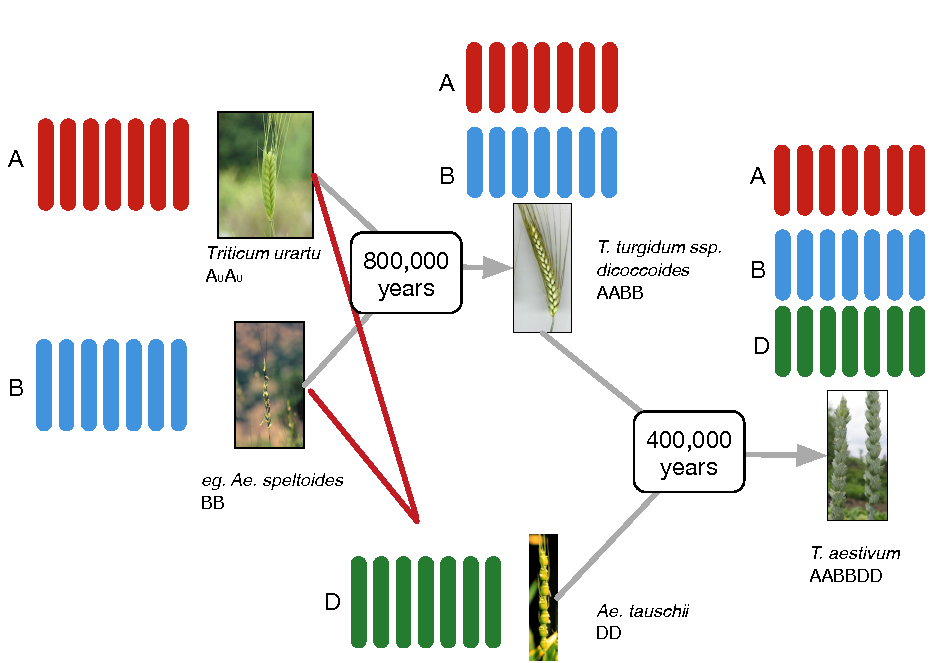
\includegraphics[width=1\textwidth]{LitReview/Figures/WheatPolyplodization.pdf}
  \caption{Hibridizations that lead to bread wheat \textit{T. aestivum}.  }
  \label{fig:lit:polyplody}
\end{figure}
Because bread wheat contains three independent copies of its genome, the expectation is to have three homoeologues for each gene. 

\unsure{Talk about paralogues. }

\subsection{Genetic Linkage}


\subsection{Experimental lines}

In crops, genetic research usually consists on crossing individuals and study the traits of the next generation. 
The progeny of a cross is called population. 
Groups of seeds with the same genetic background are called lines. 
Plants with the same homozygous background are pure lines. 
To study particular locus experimental lines are developed, the following list describe the most common \citep{VanOoijen2013Intro}:

\begin{description}
\item[F$_{1}$] The first generation of the cross between two plants. If the progenitors are different homozygous, all the population is heterozygous.  
\item[F$_{2}$ populations] come from a single heterozygous $F_{1}$ plant that is crossed to itself (self-crossed). The progeny is segregating (Fifure \ref{fig:lit:f2} with homozygous and heterozygous individuals. This type of population is used for the experiments in Chapter \ref{yr15} and it is described in more detail in Section \ref{yr15:f2}. 
\item[Back cross lones(BC)] are used to fix a trait on a genetic background. The process starts from a plant in the $F_{1}$ with the desired genotype or phenotype. This plant is crossed again to a plant from the line used as background ($P_{1}$). The progeny are called Back Cross 1 (BC1; Figure \ref{fig:lit:bc}). A plant from the BC1 with the desired genotype is selected and crossed to $P_{1}$. The process can be repeted, and with each cross the region linked to the target locus is narrowed. 
\item[Near Isogenic Lines (NIL)] After BC6, a line is considered Near Isogenic \citep{Stam1981}. At this level of back crossing most of the genetic material is the same as $P_{1}$, except for the region linked to the trait. 
\item[Recombinant Inbreed Lines (RIL)] are used to produce homozygous lines from an $F_{2}$ population. Each plant in the population is self-crossed. The lines that show an homozygous segregation are self-crossed again. After several iterations the line is considered homozygous. \ref{fig:lit:ri}).
\item[Double Haploid Lines (DH)] are an alternative technique to produce homozygous lines it. The individuals on the $F_{1}$ population are crossed to a different plant (ie maize crossed to produce wheat DH) to simulate pollination. On natural conditions, the gamets would be aborted. The embryos are rescued and treated with colchicine to induce a genome duplication. Since the duplication come from a single gamete, the resulting plant is homozygous (Figure \ref{fig:lit:dh}).

 
\end{description}

\begin{figure}
\centering
\begin{subfigure}{0.45\textwidth}
\centering
\caption{}
\label{fig:lit:f2}
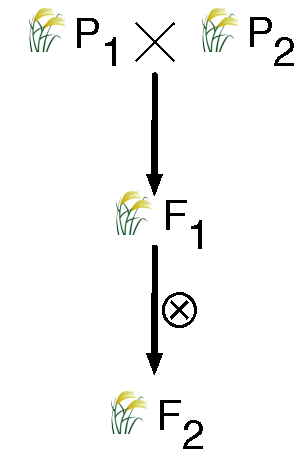
\includegraphics[height=0.20\textheight]{LitReview/Figures/crosses/F2.pdf}
\end{subfigure}
~
\begin{subfigure}{0.45\textwidth}
\centering
\caption{}
\label{fig:lit:bc}
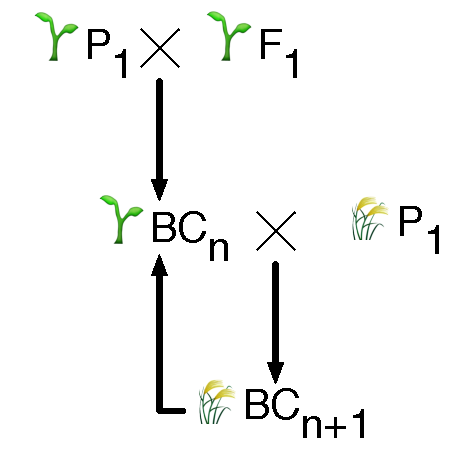
\includegraphics[height=0.20\textheight]{LitReview/Figures/crosses/BC.pdf}
\end{subfigure}


\begin{subfigure}{0.45\textwidth}
\centering
\caption{}
\label{fig:lit:ri}
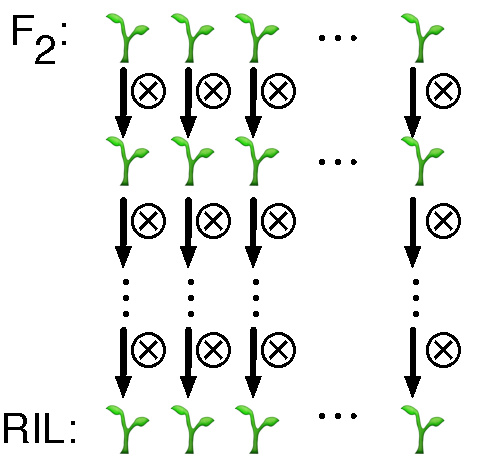
\includegraphics[height=0.20\textheight]{LitReview/Figures/crosses/RI.pdf}
\end{subfigure}
~
\begin{subfigure}{0.45\textwidth}
\centering
\caption{}
\label{fig:lit:dh}
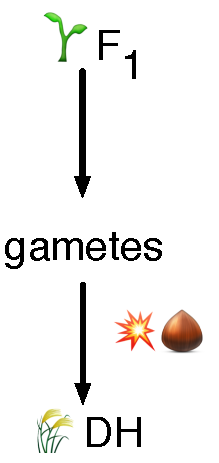
\includegraphics[height=0.20\textheight]{LitReview/Figures/crosses/DH.pdf}
\end{subfigure}

\caption[Types of experimental lines]{Types of experimental lines. 🌾 represent populations and 🌱 individual plants. $\otimes$ represent a cross between lines.$\otimes$ represent self-crosses. Ellipsis ($\ldots$) represent repetition. 💥🌰 represent a treatment to double the chromosomes from the gamete. (\subref{fig:lit:f2}) $F_{2} population$. (\subref{fig:lit:bc}) Back Cross population. (\subref{fig:lit:ri}) Recombinant Inbred Lines. (\subref{fig:lit:dh}) Double haploid}
\end{figure}

\subsection{Introgressions}

\section{Wheat Genomics}

\begin{figure}
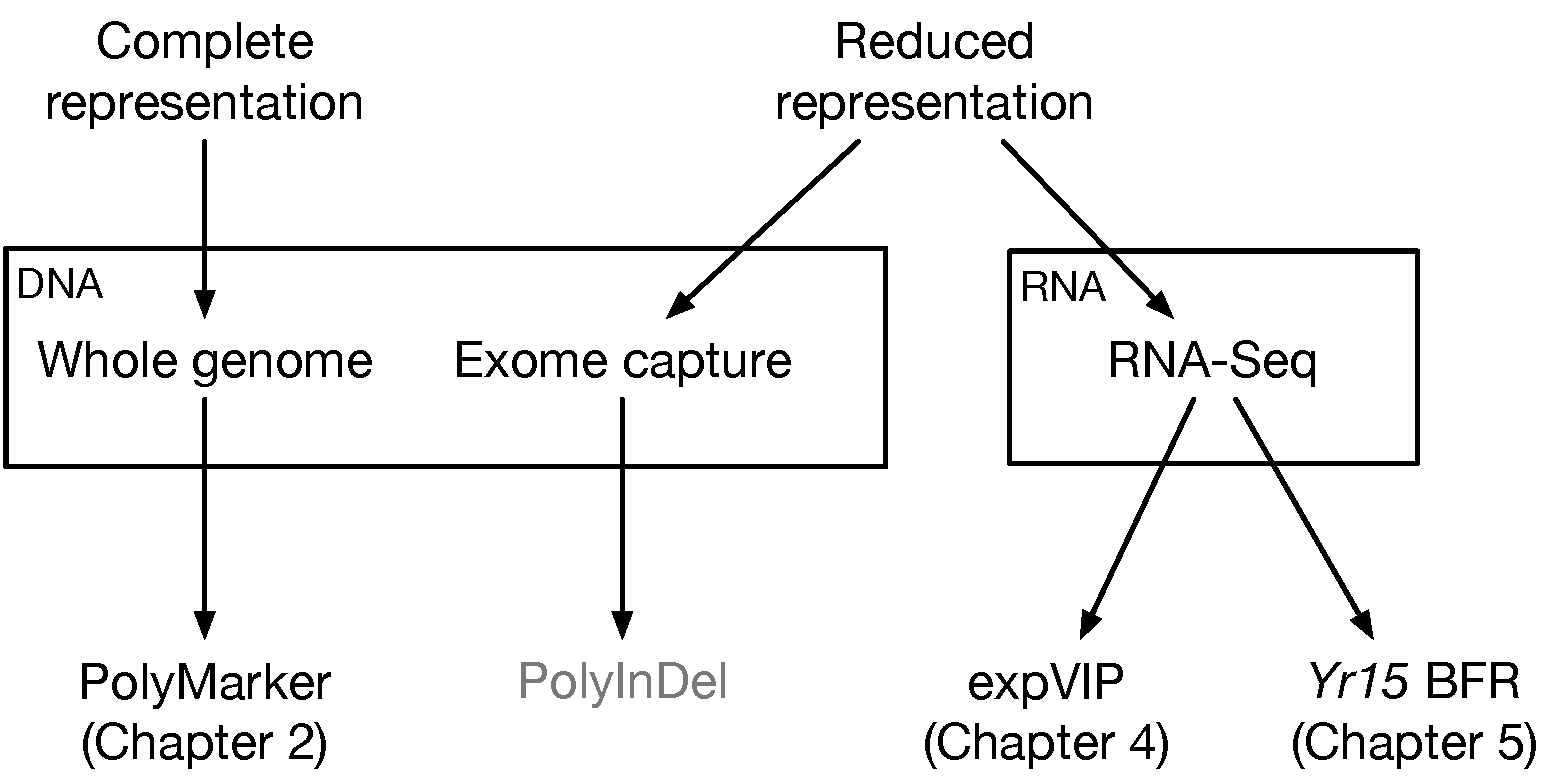
\includegraphics[width=1\textwidth]{LitReview/Figures/typesOfSequencing.pdf}
\caption{General types of sequencing ant their relationship with this PhD. PolyInDel is a project still in progress, not discussed in this Thesis. }
\end{figure}

A description of the current status of the wheat genome (\citet{Mayer2014}, \citet{Chapman2015}), the different available assemblies and and approaches to sort the scaffolds (Genome Zipper, the various genetic maps).  
\section{Sequencing} 
%The importance of the selection of the library preparation and the sequencing platforms available. A brief summary of RNA-Seq, Exome capture, Whole Genome Shotgun, etc. and on which cases are more suitable for different experiments.  Mention the new technologies developed during the years of the PhD (Ren-Seq, PacBio?)



 Sanger sequencing \cite{Lander2001} is the current gold standard in terms of quality of the sequence. It evolved from electrophoresis gels where the bands represented bases to a fully automated technique. However, the throughput is limited and doing genome wide analysis has prohibitive costs. In the second half of the 2000s high-throughput sequencing technologies emerged which had reduced the cost of sequencing. The main principle of the second-generation sequencing is to produce clusters of clones (i.e. ePCR), fix them in a plate and then add bases with a fluorescent marker. The reaction happens in parallel in millions of clusters at the same time. With each cycle, a picture is taken, showing the fluorescence of each base. Then, image processing algorithms find where in the image the clusters are and the bases are called. At this scale, the volume and complexity of the information is not trivial to manipulate, hence computing is required. 


According to the objectives of the experiment and the quality and volume of the available DNA, the library can be prepared on fragments of different sizes, the classification of the available sequencing for the fragments is the following\cite{Myllykangas2012,Metzker2010,Shendure2008,Hutchison2007}:

\begin{description}
\item[Single end] When the fragments are short, it is possible to just sequence from the 5'-end the read.
\item[Read Pairs] When the sample consists fragments of up to 500bp, it is possible to read the 5' end up to the read length were the quality starts to drop, the molecule can be turned upside down, reverse complemented and sequence backwards. It is not required, but ideally, the fragments sequenced with read pairs should be selected to have an homogenous size. The reads are in opposite orientation relative to each other. 
\item[Overlapping Read Pairs] are a variation to read pairs, where the size of the fragment is shorter than two times the read length. This allow an alignment between the two fragments to get an longer read with the limitations of the instrument.
\item[Mate pairs]  are used to get reads separated at distances between 1kbp and 5kbp. To achieve this, the molecule is circularised and the point were the two ends of the fragment were joint a biotin marker is inserted. Then, the molecule is fragmented again and the fragments containing the biotin are sequenced in the same fashion that read pairs. The resulting reads have the same orientation.
\end{description}


There are several types of experiments that can be analysed with hight throughput sequencing, accordingly, different  protocols for the sample preparation exist. The following is a short list of some of them 

\begin{description}
\item[Whole genome shotgun]  When a sample is prepared for WGS, the DNA is extracted and chopped in fragments  and sequenced. The reads obtained are, in principle, randomly distributed across the whole genome
\item[RNA-Seq].  Instead of sequencing DNA, mRNA is captured and sequenced. The fragments are not amplified in any way, to enable a portrait of the gene expression levels. 
\item[ChIP-SEQ]. Chromatin Immunopresipitation is used to find relationships between proteins and DNA sequence. It is useful to find transcription factors and replication-related proteins.
\item[Amplicon sequencing]. Used primary to do barcoding of species. A known gene is amplified (i.e. 16S) with the intention of characterising the species present in the sample. 
\item[Metagenomic capture] From a mixed sample (soil, root, animal fluids) all the DNA is extracted and sequenced, this gives a snapshot of the microbial community in the sample
\item[RAD-seq] Restriction site associated DNA markers are useful to do population analysis. The technique focus on sequencing regions around restriction sites and the variations around them can be used to genotype individuals. 
\item[Exon capture] The DNA is extracted and baits are used to attract the regions with motif common around exons. This allows to sequence only the genes and regions near them.  
\end{description}


The different sequencing technologies available as of 2013 have different yields, advantages and disadvantages, as described bellow:

\begin{description}
\item[Illumina] Each fragment is amplified using bridge amplification over and over in the same place in the plate to form clusters. After the clusters are formed, a last cycle of amplification is carried on with the bases being added to the template, with the intervention of a polymerase, have a fluorescent marker which make the cluster glow depending on the added base. It adds one base per cycle.     With a read length between 75bp and 250bp is currently the most widely adopted platform. The As a de facto standard, many tools exist to cope bioinformatically with the biases of the machine.  The run takes 4 or 9 days, depending on days, depending if one or two reads are generated for each fragment. It produces up to 35 gigabases per run. 

\item[SOLiD] The preparation of the fragments is similar to Illumina, however, when adding the bases they are added in pairs. This technique is called sequencing by ligation as it use a DNA Ligase, as opposed to a polymerase, to determine the transition between bases. The resulting sequence is not in base space, but in colour space, which represents the transition state between bases. This technique is robust for finding SNPs when you have a good reference where to align the reads. However, the number of tools available and the research done to analyse sequences in colour space is low compared to the tools using base space. The runs take between one and two weeks to complete, with a yield of up to 50 gig abases per run. The read length can be up to 50 bases

\item[Roche/454] The fragments are cloned in beads, which then fall in wells in the slide. The sequencing is done by adding nucleotides in a determined order. The next nucleotides to be added in the reaction contain a fluorescent marker. The bases are not added one by one, but all the bases that are the same are added together. The amount of glow on each well can tell how many times a base is added. As the glow is not a discrete number, when a long homopolymer appear (above 5 bases) the likelihood of having a wrong count of the homopolymer is increased.  The average read length varies between 300 and 700bp. A run usually takes half a day, but it only yleds 0.45 gigabases. The cost of the reagents is relatively expensive, but if the experiment requires longer reads it is a good option. 

\item[PacBio] Opposed to all the previous technologies, Pacific Biosciences has developed a sequencing technology where the molecules doesn't need to be PCR amplified before the sequencing. The glass slide used contains wells with a depth of 100nm where a polymerase lays at the bottom. The nucleotides to be added have a fluorescent marked that is freed when the polymerase adds the nucleotide, releasing a light signal, which then can be captured from the bottom of the glass. The error rate for this technology is still high (about 10\% of the bases are miscalled), however reading several times the same molecule reduce the error rate. The main advantage is that the reads can be over 1kbp. 

\item[OpGen] Additionally, high-througput optical mapping technologies, like OpGen, are becoming accessible.  The maps are done by fixing single molecules of DNA are held on a slide. Then,  restriction enzimes targeted to specific digestion sites cut the fragment and fluorescent markers are added to the ends of the fragments. Finally, the fragments are visualised and the size of the molecules is measured by the distance between fluorescent points in the slide. This is done with several fragments at the same time. Then, the distances between restriction sizes can be compared across all the fragments to generate a consensus. Finally, if you have contigs from other technologies, it is possible to complement the information and get better assemblies. Even without the contigs, the data can be used to compare translocations within strains of different bacteria or homologous species at a chromosome level. 

\item[ION Torrent] (Do some research on newer sequencing things)

\end{description}

\section{Sequence analysis}
This section discusses the criteria to decide analysis done after sequencing, when to do re-alignments or \textit{de novo} assemblies, how to do SNP calling in diploid and polyploid organisims and the bulk frequency ratios.  



DNA sequence alone is not alone to enough to understand the biology behind, a context is required. There are databases like Ensembl and NCBI that act as repositories of the known public sequences. 

From the computational point of view, the problem can be viewed as a string matching. The Smith-Waterman\cite{Smith1981} and Needleman-Wunsch\cite{Needleman1970} algorithms are the gold standard interns of accuracy looking for similarity between sequences. However, the execution time for both of them is prohibitive to run in massive databases. The algorithm execution time is O(mn), as it requires calculating a matrix of size $mn$ where $m$ is the target sequence and $n$ is the query sequence.  To scale this to a manageable problem algorithms like BLAST index the references and use heuristics to make the search more manageable, with some penalty in the accuracy. This alignments tools are useful for long stretches of DNA (like cDNA or contigs)\cite{Altschul1990}.

TODO: List of global aligners
-BLAST
-BLAT
-Exonerate
-nucmer

-MAFFT
-Clustal


When looking at a protein level, where the sequences may be only loosely similar, Hidden Markov Models (HMM) are used to search for protein families. This can be useful to annotate putative proteins and their functions. HMMs require a training dataset, where proteins are previously annotated and the reference is a model encoding the characteristics of a family, with associated probabilities. Hence, this technique is something between a sequences aligner and a classifier\cite{Eddy2004}. 

When analysing high-throughput sequencing, having millions of short sequences make unfeasible to try to align the data to every possible reference. However, one can take in advantage the fact that you know which organism you are looking for and, if available, use a genomic reference. For this, tools like MAQ, BWA, Bowtie, among others, provide indexed search.  Once you have your reads aligned to a reference you can do more analysis, depending on the biological question being asked and the type of sequencing carried on.  Fortunately, most of the Short-Read sequence alignment produce similar outputs and the SAM format is becoming a de facto standard. This is allowing to make more modularised downstream analysis where you can test different aligners with different settings and pick the algorithm that better fits your experiment\cite{Liu2012,Li2009,Li2009a}. 

\subsubsection{Ambiguity Codes}
\label{lit:ambiguity}
Make a table with the ambiguity codes and why they are useful. 




\subsection{RNA-Seq}
\label{lit:RNASeq}

One way to narrow down which genes are involved in certain trait or response to the environment is to focus on studying only the expressed genes. One of the techniques involving high-throughput sequencing is RNA-Seq. This technique captures the messenger RNA in the tissue being studied and sequenced. The premise is that you will find a gene more expressed if it is being used by the organism. Some proteins with a vital role for the cell are always expressed (i.e. RuBisCO for carbon fixation in plants\cite{CooperGM2000}). On the simplest of the experiments you would need two datasets to compare, one with the gene being looked expressed and one where it is not. The expression can come from different environmental conditions, development stage or different genotypes.\cite{Mortazavi2008} 

Depending on how much \textit{a priori} information of the analysed organism is available different bioinformatic approaches can be used.
\begin{description}
\item[Transcriptome alignment] The reads are aligned to a database of known cDNA. Ideally, alternative splicing sequences are available, so a simple alignment should work (i.e. BWA, bowtie). 
\item[Genomic alignment] The reads are aligned to the genome. The splice junctions, introns and axons need to be accounted, so simple alignment doesn't work. Regular alignments are used, but the reads may be trimmed at fixed sizes to allow discontinuous alignments using regular tools (i.e. Stampy, tophat/cufflinkns)
\item[\textit{De Novo} transcriptome assembly] If a reference of the organism is not available, it is possible to generate a draft transcriptome with the RNA-Seq reads with traditional assemblers (velvet, abyss) or with specialised assembler tools like Trinity. 
\end{description}

Once you have the alignments it is possible to evaluate the relative expression of the genes in the sample calculating the Reads per Kilobase per Million mapped reads (RPKM) or the Transcripts per Million (TPM). This normalises the expression by the amount of sequenced data and can be used to find which genes change in expression volume across different samples.   
%TODO: Write more details of RPKM vs TPM


\section{Wheat specific resources resources}
\label{lit:wheatResourcers}


\subsection{Gene models}
-UniGene
-UCW Gene models
-Gene annotation IWGSC
-Gene annotation TGACv1

\subsection{Genetic markers}


Markers
-90k
-820k
-MASwheat/SRR

\subsection{Genetic maps}
Genetic maps
-Wang
-Chapman/PopSeq (is the same population, improved)

\subsection{Genomic sequence}
Assemblies
-Chapman
-IWGSC
-TGACv1
-NRGene (unpublished?)
-454 Liverpool

\subsection{Online resources}
Portal
-CeralsDB
-MASWheat
-Ensembl
-Wheat-expression
-Copo

The Collaborative Open Plant Omics (COPO; \citealt{Davey2015}) is a an initiative to integrate data from different databases. 
The idea is to improve the interaction across repositories trough an \gls{api}, a standard way to ensure the interoperability between systems. 
This approach keeps the responsibility of the system and data maintenance on the service providers. 
Service providers must ensure the compliance to standard of curation and integration, which would simplify the data analysis and visualisation, and ultimately promote the use of the integrated resources.  



%A compilation of the currently available resource for whet genetics and genomics. MAS wheat, CeralsDB, Ensembl, etc.  



%\section{Computer Programming}
%Why Ruby and javascript?
%-Ruby
%-BioRuby
%-JavaScript
%-BioJS
%-Rails. 
%-SQL
%-D3%

%-lamda functions
%-functions/methods

\subsection{Computer science used for this thesis}

The following subsections give a brief overview of computer science concepts used in the thesis for the development of PolyMarker (Chapter \ref{cha:polymarker}), expVIP (Chapter \ref{cha:exp}) and, the algorithms for the data analysis for the marker development for \acrshort{yr15} (Chapter \ref{yr15}).  

\subsubsection{Functions}

\subsubsection{Hash tables}

\subsubsection{Object Orientated}

\subsubsection{Web development vs desktop development}










-Containers, as in AWT. 

 \label{lit:patterns}
%!TEX root = ../Main.tex

\chapter{PolyMarker: A fast polyploid primer design pipeline}
\chaptermark{PolyMarker}
%\section{Introduction} 
%Explain how the SNP markers are designed without the tool and an overview. 
One of the main challenges of working with polyploid species is the design of genome specific molecular markers. 
This is particularly true when targeting conserved homoeologue regions, where a primer could bind to a pair,or triplet, of identical sequences. 
For that reason, designing primers for polyploids require to include bases that are specific to the target, in addition to the physicochemical properties of the primer.  
The traditional methodology to find primer candidates include a blast search and a local alignment, select the primer candidates manually, and finally, validate the primers with a tool, like \verb|Primer3| \citep{Rozen}. 
To reduce the time invested in designed primers I have developed PolyMarker \citep{Ramirez-Gonzalez2015a}, a pipeline to automate the primer design for polyploid organisms.  

\section{Pipeline}

\begin{figure}
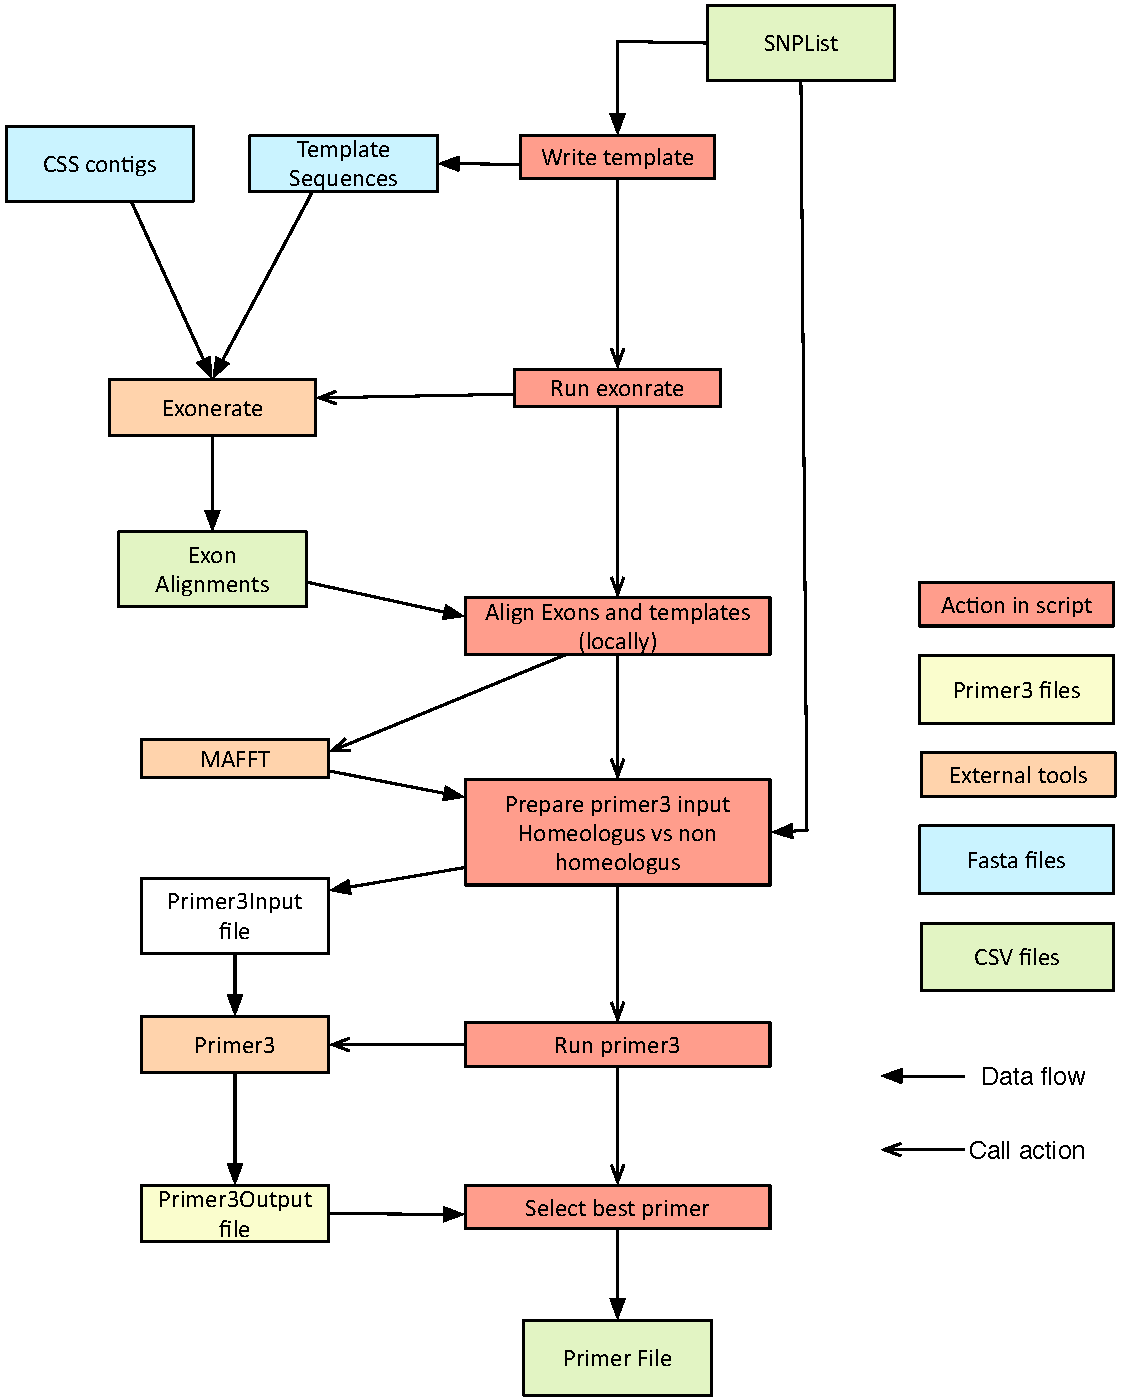
\includegraphics[width=1\textwidth]{PolyMarker/Figures/pipeline.pdf}
        \caption{Steps and tools called by PolyMarker. The colour of the boxes represent: the step is an action inside the script(red); actions of the script(orange); temporary files(yellow); inputs(blue) and; outpus(green)}
        \label{fig:poly:pipeline}
\end{figure}

PolyMarker is an automated pipeline that takes as input a list of SNPs and a reference file and produces a list of primer triplets for SNP genotyping. 
The list of SNPs is first converted to a \verb|FASTA| file with ambiguity codes \citep{Cornish-Bowden1985} 
The template sequences are aligned with \verb|exonerate| \citep{Slater2005}  to find the homoeologous regions to the target sequence. 
Then, the alignment between homoeologues is refined using \verb|MAFFT| \citep{Katoh2013}. 
A list of candidate variations is produced and used as input for \verb|Primer3| \citep{Rozen}. 
Finally, the output of \verb|Primer3| is parsed to find the best primer pair that contains a the targeted SNP and a base that is specific to the target genome (Figure \ref{fig:poly:pipeline}).  
The pipeline is written as a Ruby script, using parsers and wrappers from BioRuby \citep{Goto2010} and bio-samtools \citep{Etherington2015,Ramirez-Gonzalez2012}. 
The software is open source and released as a biogem \citep{Bonnal2012}, \verb|bio-polyploid-tools|, the source code is available in github: \verb|https://github.com/TGAC/bioruby-polyploid-tools|.


The PolyMarker input consist on SNP list with: unique name for the marker, the target chromosome and the sequence for the marker. 
The alternative alleles are surrounded by square brackets within the sequence. PolyMarker can take a list of several markers and design them in batch (Figure \ref{fig:poly:input}). 
A \verb|FASTA| file is produced with all the template sequences, with the alternative alleles substituted by the IUAPC ambiguity codes \citep{Cornish-Bowden1985}. 
The flanking sequence surrounding the SNP is limited by default to 100bp to reduce the search time and avoid missing regions that diverge near the SNP, as when the variation is near an intron-exon junction. 
%%TODO: Should we elaborate more here? 

\begin{figure}
    \centering
    \begin{subfigure}[b]{0.8\textwidth}
        \caption{}
        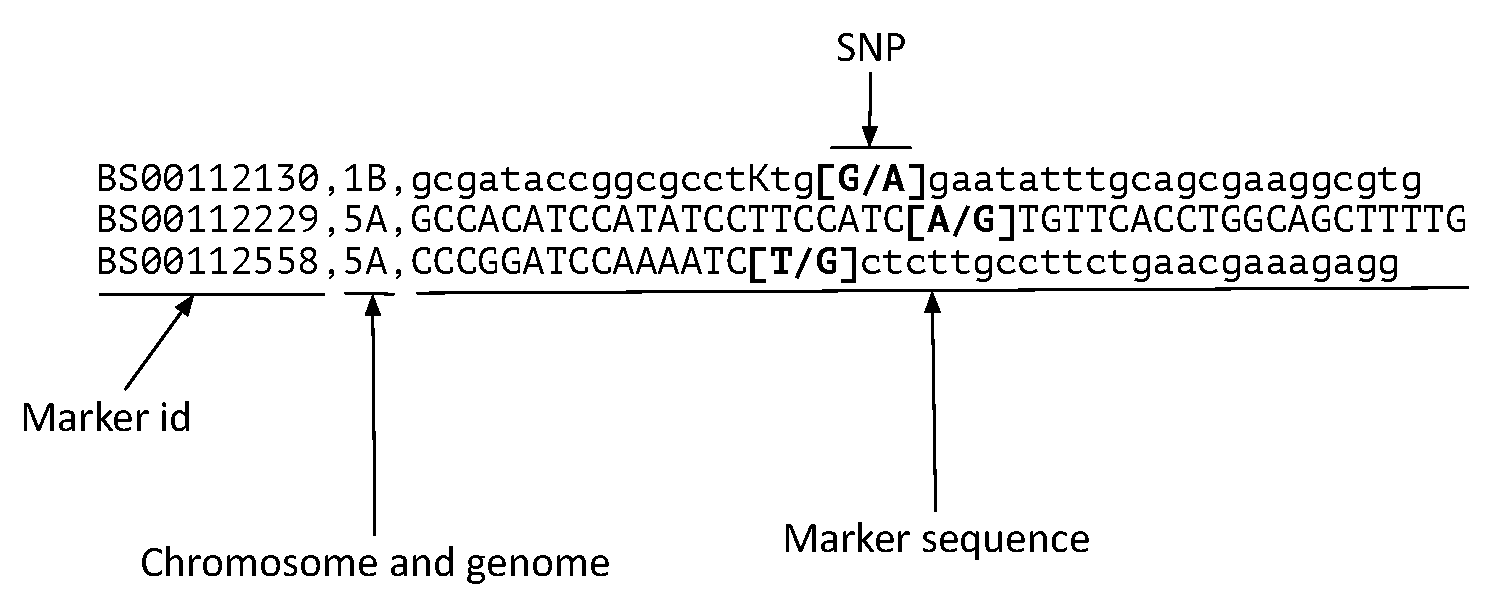
\includegraphics[width=1\textwidth]{PolyMarker/Figures/aln/input.pdf} 
        \label{fig:poly:input}
    \end{subfigure}

    \begin{subfigure}[b]{0.4\textwidth}
        \caption{}
        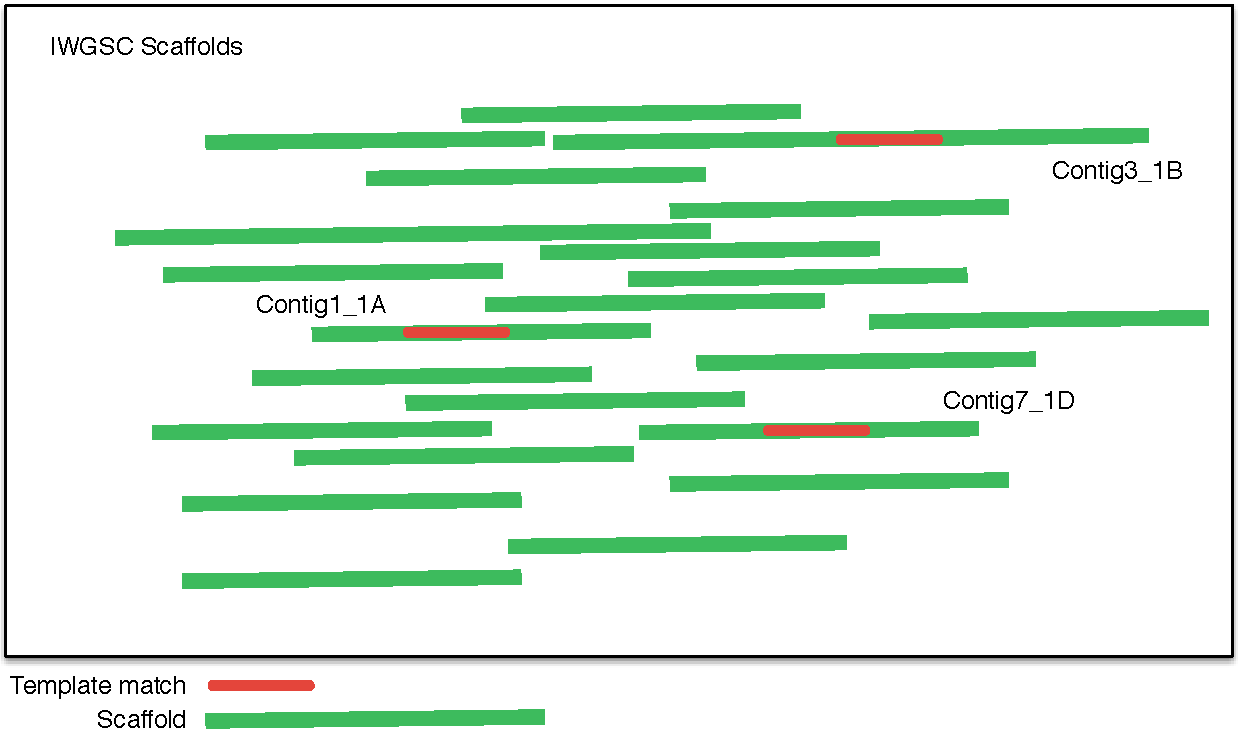
\includegraphics[width=1\textwidth]{PolyMarker/Figures/aln/scaffoldsSearch.pdf}
        \label{fig:poly:globalSearch}
    \end{subfigure}
    ~ %add desired spacing between images, e. g. ~, \quad, \qquad, \hfill etc. 
      %(or a blank line to force the subfigure onto a new line)
    \begin{subfigure}[b]{0.4\textwidth}
        \caption{}
        \raisebox{10mm} { 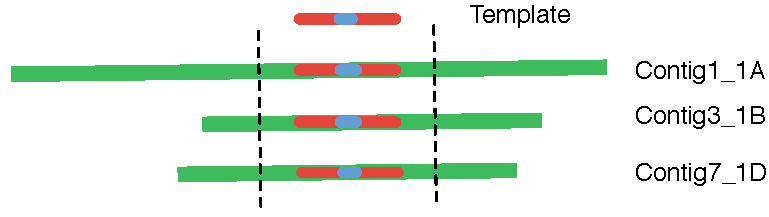
\includegraphics[width=1\textwidth]{PolyMarker/Figures/aln/scaffoldsFoundAround.pdf} }
        \label{fig:poly:globalAround} 
    \end{subfigure}
    
    \begin{subfigure}[b]{0.4\textwidth}
        \caption{}
        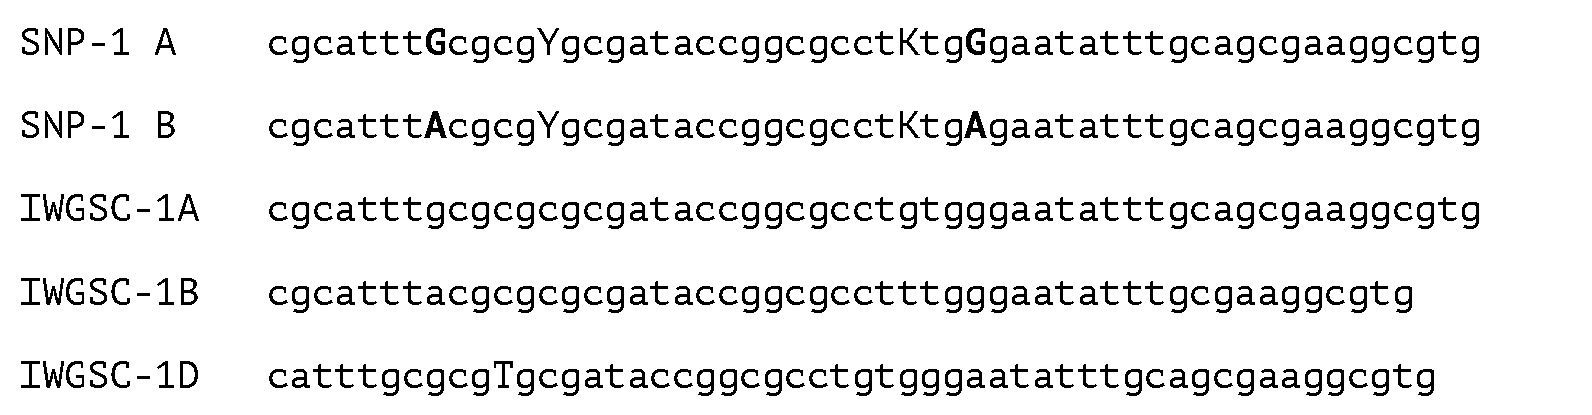
\includegraphics[width=1\textwidth]{PolyMarker/Figures/aln/scaffoldsFound.pdf}
        \label{fig:poly:globalSequence}
    \end{subfigure}
    ~ %add desired spacing between images, e. g. ~, \quad, \qquad, \hfill etc. 
      %(or a blank line to force the subfigure onto a new line)
    \begin{subfigure}[b]{0.4\textwidth}
        \caption{}
        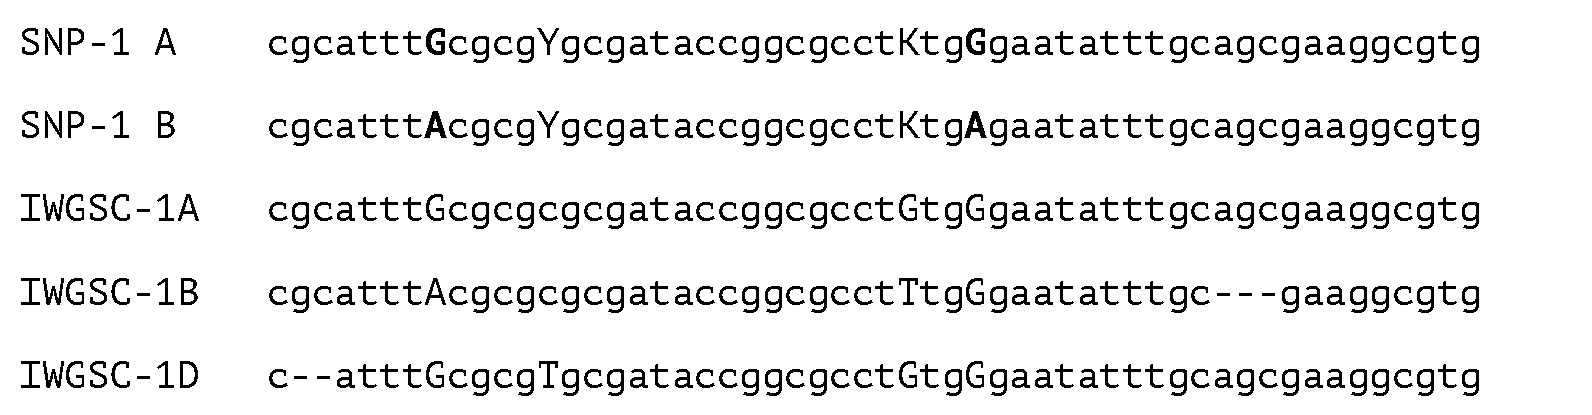
\includegraphics[width=1\textwidth]{PolyMarker/Figures/aln/localAlignment.pdf}
        \label{fig:poly:localSequence}
    \end{subfigure}

    \begin{subfigure}[b]{0.8\textwidth}
        \caption{}
        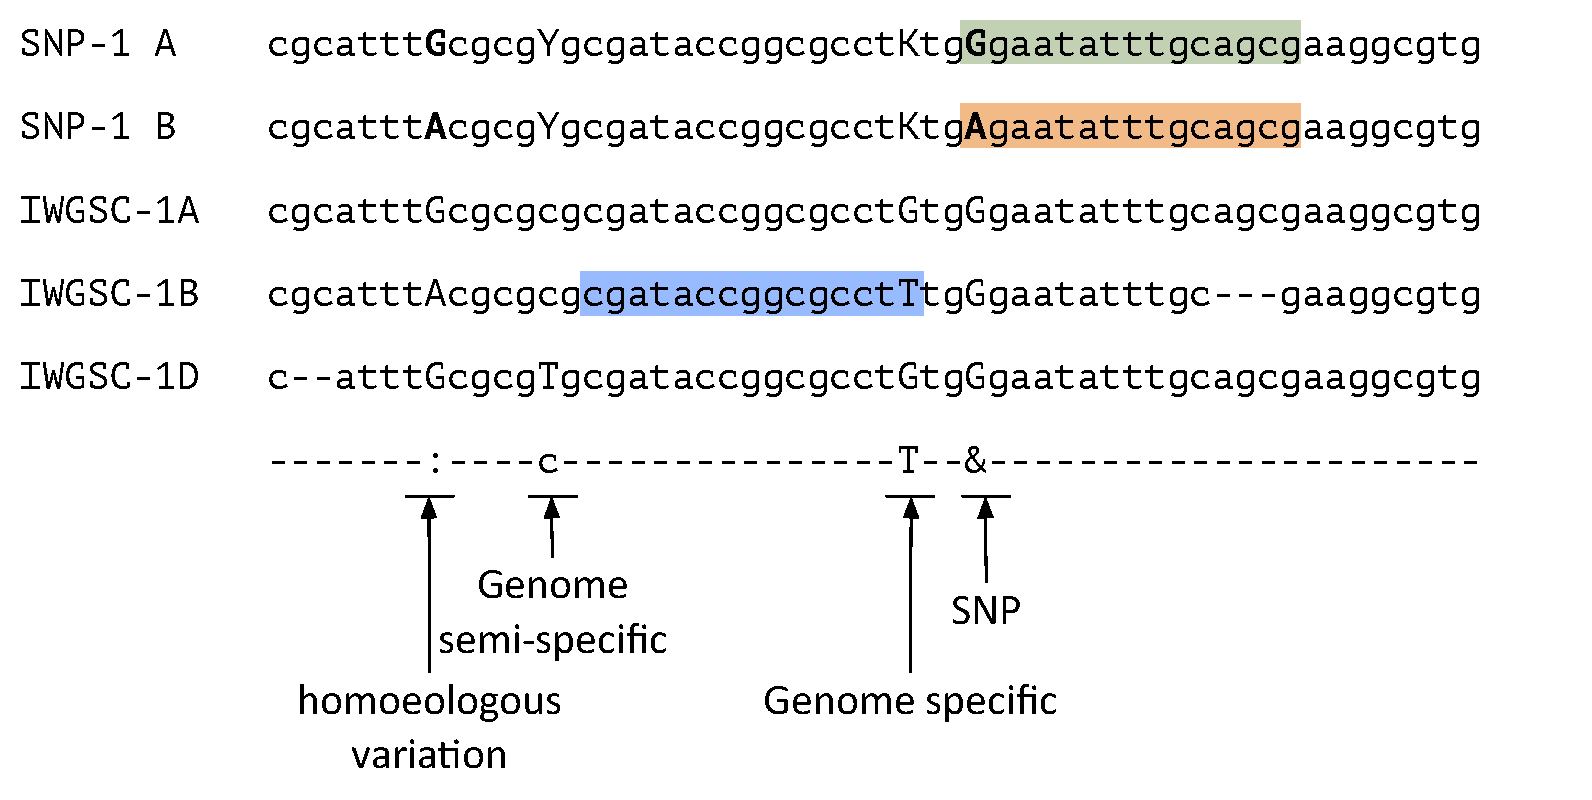
\includegraphics[width=1\textwidth]{PolyMarker/Figures/aln/mask.pdf} 
        \label{fig:poly:mask}
    \end{subfigure}
    \caption{Alignments done by PolyMarker.(\subref{fig:poly:input}) input. The alternative alleles are sorrounded by brackets. (\subref{fig:poly:globalSearch}) Global search of templates in the reference contigs. (\subref{fig:poly:globalAround}) Selected regions around the SNP on every chromosome. (\subref{fig:poly:globalSequence}) Sequence of found regions around the SNP. (\subref{fig:poly:localSequence}) Local alignment on regions around the SNP detects indels. (\subref{fig:poly:mask}) Alignment with mask and primer candidates.}
    \label{fig:global}
\end{figure}

The template sequences are aligned to the reference using \verb|exonerate| (\citealt{Slater2005}; Figure \ref{fig:poly:globalSearch}). 
The alignment is refined with the \verb|--model est2genome| option, to allow the search of sequences coming from transcripts, a common source of SNPs \citep{Allen2011}. 
The exonerate output is formatted with the \verb|--ryo| (roll your own format) to get an output easy to parse. 
All the hits that contain the SNP are extracted from the reference with a flanking sequence that extend out of the hit, by defualt, to 100bp on each side of the SNP, Figure \ref{fig:poly:globalAround}.
The size of the flanking sequence can be set to different sizes to allow the design of different types of primers. 
Different homoeologues may contain small indels, Figure \ref{fig:poly:globalSequence}. 
To enable a comparasion base-per-base, a local alignment with \verb|MAFFT| \citep{Katoh2013} is produced, Figure \ref{fig:poly:localSequence}. 

PolyMarker searches across each base in the local alignment to identify the variations across homoeologues and the target marker.
A mask is produced to highlight the bases with a variations, Figure \ref{fig:poly:mask}, on the following categories:
\begin{labeling}{Non-homoeologous}
%\begin{description}[align=right,labelwidth=4cm]
\item [Specific] Homoeologous polymorphism which is only present in the target genome (upper case).
\item [Semi-specific] Homoeologous polymorphism which is found in 2 of the 3 genomes, hence it discriminates against one of the off-target genomes or when not all the homoeologous sequences were found (lower case).
\item [Non-specific] No variation is found across homoeologues (\texttt{-}).
\item [Homoeologous] The target SNP is present across different chromosomes, so candidate SNP markers on this category are not expected to be reliably identify the allele (\texttt{:}).
\item [Non-homoeologous] The target SNP is not present across chromosomes, so it can be used to identify an allele (\texttt{\&}).
%\end{description} 
\end{labeling} 

PolyMarker was designed to produce SNP assays for KASP genotyping \citep{LGC}, which requires a common primer and two allele-specific primers. 
The common primer is selected to start on a position from a: Specific; Semi-specific or; Non-specific, on that priority. 
This means that the common primer will be as specific as possible in the region. 
For the allele-specific primers, the starting position of the primer is on the base with the SNP. 
To ensure that the stability of the candidate primers will be met, the putative starting positions are tested with \texttt{Primer3} \citep{Rozen}. 

%%TODO: check for 3primer/ 5 primer instead of starts 
PolyMarker was designed and validated with the markers described in section \ref{yr15:geneticMap}. 
For wheat, PolyMarker uses the contigs from \cite{Mayer2014}, as deposited in Ensembl. 
As new releases of the wheat genome are made available, different parsers to assign the chromosome to each sequence can be added with little effort to PolyMarker. 




\section{Applications of PolyMarker}

PolyMarker is not restricted to wheat or to KASP assays, the source code is flexible and can be extended for other types of analysis. 
On each of the following projects, PolyMarker has been adapted to design primers in species where KASP hasn't been used before, the primers are used for regular PCR amplification, or the use of KASP is not the conventional SNP calling. 

\subsection{KASP assays for public sets of SNPs} 

PolyMarker was used to design KASP assays for the 81,587 markers from \citep{Wang2014}, available on the PolyMarker website and in CeralsDB \citep{Wilkinson2012}. 
Of those markers, 40,267 where designed using the target chromosome using the genetic map published by the genetic map. 
Genes without a genetic position were aligned to scaffolds sorted by chromosome from the International Wheat Genome Sequencing Consortium \citep{Mayer2014} with BLAT \citep{Kent2002} and the best hit was selected as putative location. 
97.5\% of the assays where designed and 76\% of them are semi-specific or specific, thereby improving their expected performance with respect to randomly designed primers (Table \ref{tab:poly:designed}). 
A subset of the designed assay was used to genotype a mapping population to find resistance to Fusarium head blight \citep{Burt2015}. 

\subsection{SNPs in a mutant population}

PolyMarker was used to design primers to validate SNPs in a Targeted Induced Local Lesions in Genomes (TILLING) population, an approach to identify the function of genes by mutating them. 
To calibrate the SNP calling, KASP assays were designed to get the mutations from $M_{2}$, $M_{3}$ and, $M_{5}$ mutants \citep{King2015}. 
%TODO: Add more details as suplemental?
Then primers were designed for the whole mutant population, consisting of 1,200 Cadenza (Hexaploid) and 1,535 Kronos (Tetraploid) wheat lines \citep{Krasileva2016}. Genome-specific primers  172 and 80 SNP assays on 19 and 8 $M_{4}$ Cadenza and Kronos lines respectively. 
Of those, 71(85.5\%) Kronos and 147(88.8\%) of the Cadenza primers where valid assays (Tables \ref{app:PolyMarkerM4ValidationCadenza} and \ref{app:PolyMarkerM4ValidationKronos}).  

\subsection{Deletions on a mutant population}
%Algorithm to produce KASP for deletions in polyploids. 

\begin{figure}
    \centering
    \begin{subfigure}[b]{0.45\textwidth}
        \caption{}
        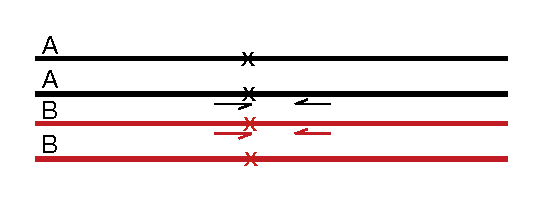
\includegraphics[width=1\textwidth]{PolyMarker/Figures/deletions/wt.pdf}
        \label{fig:poly:wt}
    \end{subfigure}
    ~
     \begin{subfigure}[b]{0.45\textwidth}
        \caption{}
        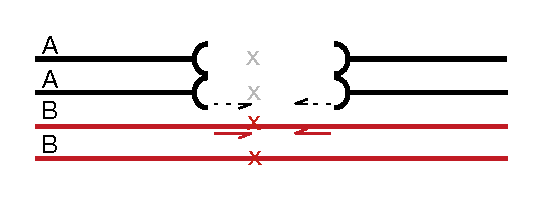
\includegraphics[width=1\textwidth]{PolyMarker/Figures/deletions/homM4.pdf}
        \label{fig:poly:homM4}
    \end{subfigure}
    \begin{subfigure}[b]{0.3\textwidth}
        \caption{}
        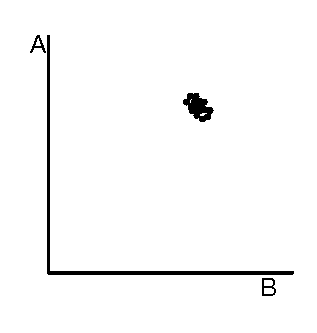
\includegraphics[width=1\textwidth]{PolyMarker/Figures/deletions/homFalse.pdf}
        \label{fig:poly:homFalse}
    \end{subfigure}
    ~
    \begin{subfigure}[b]{0.3\textwidth}
        \caption{}
        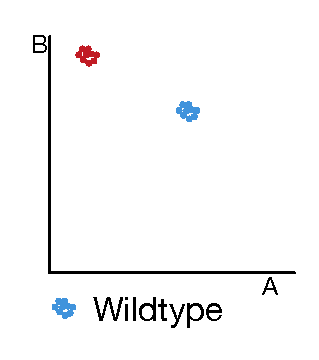
\includegraphics[width=1\textwidth]{PolyMarker/Figures/deletions/homReal.pdf}
        \label{fig:poly:homReal}
    \end{subfigure}
    \caption{KASP assays to validate homozygous deletions. (\subref{fig:poly:wt}) Primer positions for wildtype. (\subref{fig:poly:homM4}) Primer positions on  homozygous deletion on $M_{4}$ (\subref{fig:poly:homFalse} Heterozygous amplification on wildtype, including both homoeologues. (\subref{fig:poly:homReal}) Homozygous amplification on deletion line, only the non-deletad homoeologue is amplified. }
\end{figure}

On some of the TILLING mutant lines long deletions were detected \citep{Krasileva2016}.
To validate the deletions is possible to use KASP assays to produce primers that amplify homoeologues.  
PolyMarker was modified to search for variations across homoeologues to select a common primer that will amplify two genomes (Figure \ref{fig:poly:wt}, \subref{fig:poly:homM4}). 
On lines without the targeted deletion, the amplification correspond to an homozygous assay (Figure \ref{fig:poly:homFalse}).  
When a deletion is present the results of the assay look like an homozygous sample, with the intensity of the assay towards the the conserved homoeologue (Figure \ref{fig:poly:homReal}).
A set of KASP assays for the the deletions and mutations located on the same chromosome where designed to validate 11 homozygous deletions on $M_{4}$ plants. 
In all cases the segregation of the mutations was as expected, except for a predicted heterozygous mutation that was called as homozygous. 
Also, all the KASP assays that contained a deletion were called homozygous, as expected. 
To ensure that the calls didn't come from a single cluster, 4 wildtype plants were genotyped and the markers for deletions where called as heterozygous. 
An example of a validated deletion, with the calls for each individual is shown on Table \ref{app:poly:homDelCad0423}.

\subsection{PolyMarker public web service}
To make PolyMarker accessible to the community, a web server that allow the submission of SNPs was developed. 
The web interface consists on two virtual machines, one with a web facing interface that stores the queries, and a dedicated node to submit jobs to an HPC cluster.
The on-line interface further simplifies the design of KASP assays, a process that used to take a couple of weeks now is done in a couple of hours. 
Since the release of the public service in July 2014 until August 2016, 1,739 requests to PolyMarker have been done. 
%TODO: Does this sounds like too much marketing? 


\subsection{Genotyping of \textit{Puccinia 
striiformis} f. sp. \textit{tritici} isolates.}
In \cite{Hubbard2015}, \textit{Puccinia striiformis} f. sp. \textit{tritici} (PST) isolates were sequenced and assigned to clusters, according to their genotype.
The clusters are useful to monitor the changes in the pathogen population, which can be used to predict if certain wheat lines will be resistant to the isolates in the field. 
PolyMarker was used to design primers for PST, using the assembly PST-130 \citep{Cantu2011}.
Out of 15 assays 11 can be used to identify to which cluster of isolates a sample is likely to belong, Supplemental Table \ref{app:PolyMarkerPST}.


\section{Discussion}

PolyMarker is a tool that was born as part of the validation of the SNPs found in Chapter \ref{yr15}. 
Originally, the primer design was ought to be done manually, a slow, error-prone and, repetitive process. 
The steps require the use of several bioinformatics tools, but once I figured out the steps I decided to automate the process. 
Since designing genome-specific primers is a common task in wheat research and breeding, the community showed interest on the tool and I decided to refine it and make it open source. 
PolyMarker has been used successfully in several projects and it even allowed the novel use of KASP assays to validate long deletions in polyploids. 

The current web interface of PolyMarker is limited to KASP assays, however the command line version is more flexible and has been used to design primers for PCR amplicons, capillary sequencing and on other organisms. 
The ideas behind PolyMarker had been taken by other projects like the scripts described in \cite{Ma2015} and the corresponding web interface, GSP \citep{Wang2016}. 
As new references of wheat come available, PolyMarker should be updated to work with pseudomolecules and the web interface updated accordingly.  

%Remarks on the importance of getting the primers right, and the time saved by automating the primer selection. Also mention other primer design tools that have been inspired by polymarker: \cite{Ma2015}, \cite{Wang2016}

 



%!TEX root = ../Main.tex

\chapter{Genetic map of \textit{Yr15} with RNA-Seq.}
\glsresetall
\chaptermark{Genetic map of \textit{Yr15}}
\label{yr15}
%This section describes in detail than the paper of \citet{Ramirez-Gonzalez-2014}
 
%Breeding importance of \textit{Yr15} and original source (an introgression of \textit{T. diccocoides}). 
\section{Background.}
Wheat breeding programs aim to improve the wheat lines available for production.
One of the traits desired in an elite line is the resistance to pathogens, such as\gls{pst}, the fungi responsible of yellow rust.
A source of resistance genes are introgressions from other species, such as \textit{Triticum dicoccoides} (emmer, Figure \ref{fig:lit:polyplody}). 
In the University of Sydney a collection of \glspl{nil} with introgressions to several yellow rust resistance genes on a susceptible background were developed \citep{Wellings1998}. 
In this chapter the \gls{nil} for the \textit{Yr15} locus is used to produce a mapping population to produce a mapping population, which when combined with mapping by sequencing approaches, results in improved diagnostic markers. 

%TODO: Paragraph explaining NILs
\subsection{Segregation on \texorpdfstring{$F_{2}$}{F2} populations.}
\label{yr15:f2}
Molecular markers can be used to select lines by testing if certain allele is present in a line, without the need to phenotype  the given line.
To find which regions are linked to a trait the use of $F_{2}$ mapping populations is a common practice, especially for major single gene traits.
The population is produced by crossing two (usually homozygous) parents ($P_1$ and $P_{2}$) with different alleles, A/A (dominant, resistant if containing \textit{Yr15}) and a/a (recessive, susceptible in our experiment).
When the trait is dominant and has a mendelian segregation, the $F_1$ population should exhibit the dominant trait, as it has a copy of each allele (A/a). 
The $F_1$ is then self-pollinated to produce and $F_2$ population which should segregate with a ratio of 1:2:1, dominant:heterozygous:recessive respectively.
This generates a population with a phenotypic ratio of 3:1 (resistant:susceptible), since the effect of the recessive allele is masked by the dominant allele (\citealt{VanOoijen2013}; Figure \ref{fig:yr15:f2schematic}).  

\begin{figure}
  \centering
   \begin{subfigure}{0.45\textwidth}
   \caption{}
   \label{fig:yr15:f2schematic}
   \centering
   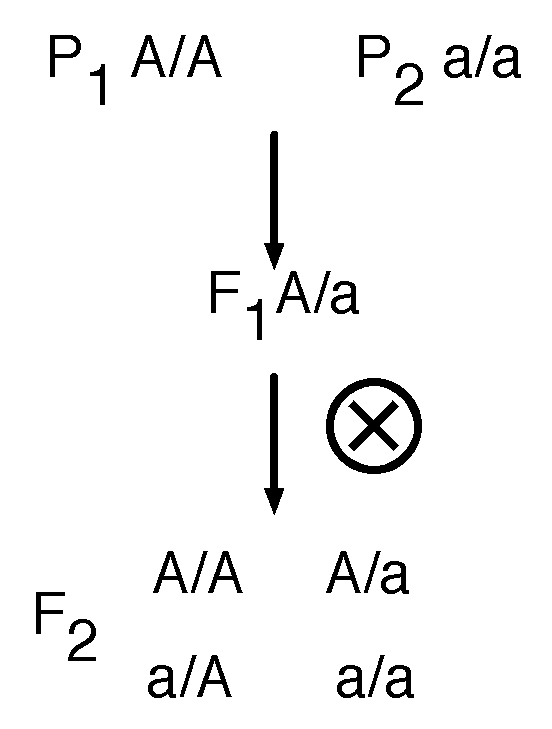
\includegraphics[height=0.3\textheight]{Yr15/Figures/population/F2schematic.pdf}
  \end{subfigure}
  ~
   \begin{subfigure}{0.5\textwidth}
   \caption{}
   \label{fig:yr15:BSAschematic}
   \centering
   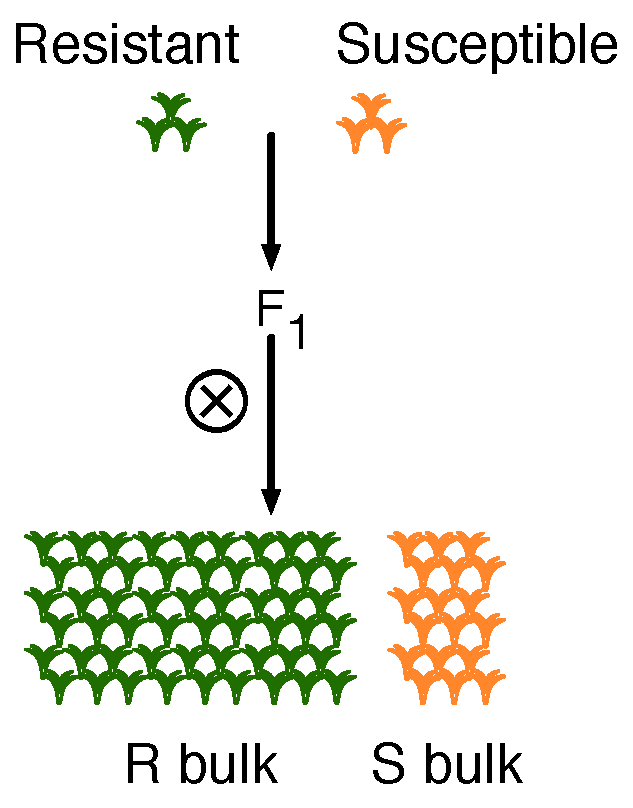
\includegraphics[height=0.3\textheight]{Yr15/Figures/BSA.pdf}
  \end{subfigure}
   \caption[Alleles on $F_2$ population and Bulk Segregant Analysis.]{Alleles on $F_2$ population and Bulk Segregant Analysis. The $\otimes$ represent self-pollination. (\subref{fig:yr15:f2schematic}) The cross of two homozygous parents, $P_{1}$ and $P_{2}$, with a dominant and a recessive allele of a gene produces an heterozygous $F_{1}$. The $F_{1}$ crossed with itself produce a segregating $F_{2}$ population with a 1:2:1 ratio (A/A:A/a:a/a). The upper and lower cases represent dominant and recessive alleles, respectively. (\subref{fig:yr15:BSAschematic}) Bulk Segregant Analysis consist on pooling DNA from the $F_{2}$ population. The DNA is mixed in bulks coming from plants with a shared phenotype. For a dominant resistance gene, an R sulk contains only resistant individuals (with A/A and A/ genotype) and, an S bulk with the susceptible individuals (with a/a genotype). } 
  
\end{figure}

\subsection{SNP calling}
\gls{bsa} consists on pooling the DNA of individuals from a segregating population with contrasting phenotypes \citep{Michelmore1991} in a segregating population. 
By combining multiple independent individuals with similar phenotypes, one can identify regions which are over-represented or enriched in the corresponding bulks. 
Regions which are not linked to the trait of interest show up as heterozygous in the bulks, whereas regions which are linked to the trait of interest will be enriched for either parental allele.
Here one would expect an enrichment of the resistant allele A with respect to the susceptible allele a in the resistant bulk. 
Analogously, one would expect the absence of the resistant allele A in the susceptible bulk (Figure \ref{fig:yr15:BSAschematic}). 
This approach can be used to identify SNPs using \gls{ngs}-based methods, such as exome capture \citep{Hodges2007}, RNA-Seq \citep{Pickrell2010}, whole genome resequencing \citep{Schneeberger2009}, among others. 

To find SNPs linked to the trait segregating in an $F_{2}$ population using \gls{ngs} data there are several options. 
In organisms with a contiguous reference genome, a normalized count of the times each allele is observed is enough to find the region linked to the trait; this simple ratio is called SNP-Index \citep{Takagi2013a}.
However, wheat is a polyploid organism, with an average identity between homoeologues of over 98\%. 
Because of the high identity, reads coming from different homoeologues may map to the same position; and this problem is exacerbated in cases where a reference sequence for some of the homoeologues is absent. 
The \gls{bfr} \citep{Trick2012} methodology can work on organisms that have more than one pseudo genome and where not all of the genes, either homoeologues or paralogues, have been characterised independently; it works with a single reference by collapsing similar regions. 
Both methodologies rely on an enrichment of the alleles linked to the trait in the corresponding locus. 

An example of homoeologous variants between two sub-genomes of wheat is the G$>$T variant at position 181; K in consensus (Figure \ref{fig:yr15:bfr}). This variant will produce the same ambiguity code for both parental consensus sequences and can therefore be excluded. 
An example of real allelic varietal SNPs between the parental genotypes is exemplified by the G$>$A variant at position 184; R in consensus. These variants are distinguished by the presence in only one of the consensus sequences. 
The allelic SNPs are then examined further with the alignments of the bulks to identify the SNPs that are enriched on the resistant plants.
The SNP index is the proportion of times an alternative allele is observed over the coverage at certain position, in the example the susceptible bulk has an SNP index of $1/8=0.125$ while the resistant bulk has an index of $6/8=0.75$ \citep{Takagi2013a}. 
The \glspl{bfr} are then calculated by dividing the SNP Index of the sample containing the target phenotype (resistance) over the sample without the trait (susceptible). For this example, it would be $0.75/0.125=6$.  
A high BFR suggests that the \acrshort{snp} is linked to the target trait \citep{Trick2012}. 
The implementation of the BFR analysis is detailed in Section \ref{yr15:sub:bfr} and the results on the $F_2$ population are discussed in Section \ref{sec:yr15:bfr}. 
%Repeated
%The Bulk Frequency Ratio (BFR) methodology can work on organisms that have more than one pseudo genome with not all the genes, either homoeologues or paralogues, characterised independently; it works with a single reference collapsing similar regions.

\begin{figure}
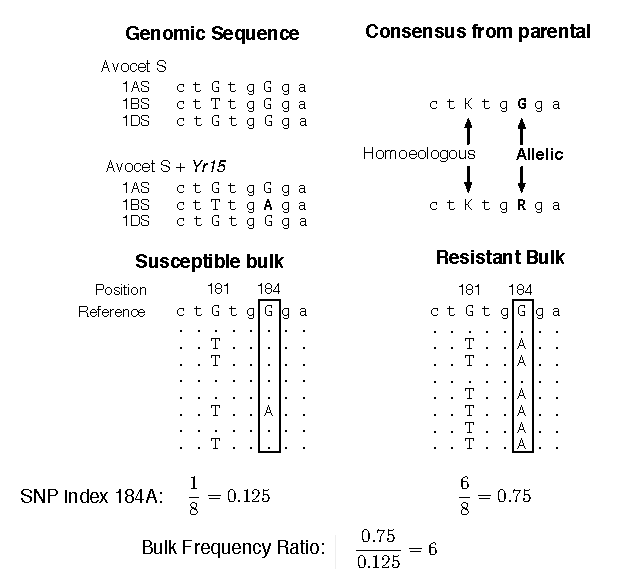
\includegraphics[width=1\textwidth]{Yr15/Figures/bfr.pdf}
\caption[BFR formula]{BFR formula. Illustration of a non-informative homoeologous SNP (G181T) present in both parental lines, and an informative allelic SNP (G184A), only present in the resistant progenitor Avocet S + Yr15. The consensus sequences from the parental genotypes include this information in the form of ambiguity codes (K and R, respectively). In the bulks, the individual reads align across the reference sequence, with matches indicated by dots, and polymorphisms at positions 181 and 184 indicated by the corresponding nucleotide variants. The SNP index is calculated as the frequency of the informative allelic SNP in each bulk. The Bulk Frequency Ratio is the quotient of the resistant and susceptible bulk SNP Indexes. Figure previously published in \citet{Ramirez-Gonzalez2015c}. }
\label{fig:yr15:bfr}
\end{figure}

To call SNPs from RNA-Seq, a reference transcriptome rather than a reference genome sequence is used as target to align the reads. 
The UniGenes database, from NCBI, contains the known genes of each species with all the variations of each gene automatically collapsed and represented with the longest available \acrshort{cdna} \citep{PontiusJUWagnerL2002}. 
The \acrshort{ucw}  gene set described in \citet{Krasileva2013} contains 94,177 models from tetraploid and hexaploid wheat, assembled and phased to separate different homoeologues. 
Both gene sets complement each other, however, the \acrshort{ucw} gene models should provide an improved alignment, since the different homoeologues have not merged in a single model - a possible side effect of the UniGene pipeline. 

\subsection{\textit{In Silico} mapping.}
There are several layers of information that can be used to add a context to the SNPs. 
When the SNPs are called from genes like the UniGenes \citep{PontiusJUWagnerL2002} or the UCW gene models \citep{Krasileva2013}, the location of the genes can be assigned by aligning them to a genomic reference, even if it is fragmented. 
A source to get the order of the scaffolds are previously published genetic maps, such as the one described in \citet{Wang2014}, which has the sequence of the markers available.
The markers and the genes can be aligned to the scaffolds with a high identity cutoff (over $98\%$), to avoid them being assigned to a homoeologue or paralogue on a different chromosome.
The practice of using genetic maps to sort genomic sequence and produce pseudo-chromosomes is common in genome wide projects, and is usually performed with \textit{ad-hoc} tools \citep{Tang2015}.
The highly fragmented state of the \acrshort{css} assembly prevents the use of genetic maps to produce pseudomolecules, as those maps which are currently available do not have enough resolution.
However, they are dense enough to sort the scaffolds in bins when several markers map to the same location. 
In this way, it is possible to use the scaffolds as a proxy to map the genes to their genetic position (Figure \ref{fig:yr15:layersOfMapping}).
The results of mapping the genes with SNPs to the CSS assembly and the genetic map are described in Section \ref{sub:yr15:inSilico}. 
For a longer description of resources available for wheat see Section \ref{lit:wheatResourcers}.
%\unsure{To do: section talking about genetic map. }
%\unsure{To do: Microsatellites vs SNP markers. }

\begin{figure}
  \centering
  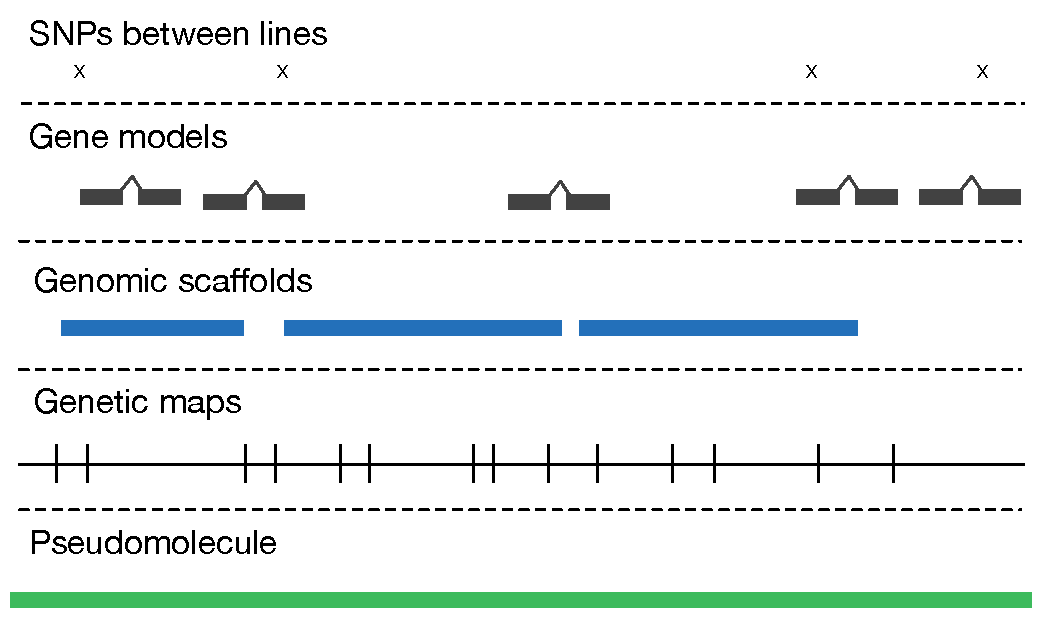
\includegraphics[width=1\textwidth]{Yr15/Figures/mapping/layersOfMapping.pdf}
  \caption[Layers of information to do \textit{In Silico} mapping.]{Layers of information to do \textit{In Silico} mapping. SNPs are called from gene models. The genes and markers from genetic maps are aligned to scaffolds. The order of the markers in a genetic map can be used to sort the scaffolds.} 
  \label{fig:yr15:layersOfMapping}
\end{figure}

Finally, the best candidate SNPs were selected to produce a genetic map which lead to a triplet of markers diagnostic for the target locus. 

The steps described in this chapter were first published in \citet{Ramirez-Gonzalez2015c} and the results of this chapter are published in \citet{Ramirez-Gonzalez2015b}.

\section{Mapping population.}

The population was developed by crossing the resistant line \gls{yr15} \citep{Wellings1998}, Figure \ref{fig:yr15.yr15Photo}, to the susceptible line \gls{avs}, Figure \ref{fig:yr15:avsPhoto}. 
\gls{yr15} is a \gls{nil} of a 6th generation \gls{bc} and the \gls{avs} background is highly susceptible to yellow rust, hence the resistance is conferred by the \gls{yr15} locus. 
$F_{2}$ seeds from three independent $F_{1}$ plants where sown and tissue was collected before fungal inoculation to avoid the effect of the disease resistance response on gene expression. 
Sampling after inoculation could have led to associations in the bulks due to expression of genes downstream of \gls{yr15} and not due to the gene itself.
Seedlings were challenged at the three leaf stage as it is known that \textit{Yr15} confers resistance in seedlings \citep{Gerechter-Amitai1989}.
The expected segregation of a $F_{2}$ population is 3:1 (resistant:susceptible), since \textit{Yr15} is a dominant gene.
From the 232 plants in the $F_{2}$ population that germinated, 187 were resistant and 45 were susceptible, which deviates slightly from the expected ratio ($\chi^{2}=0.049$).
Segregation distortion has been shown for the same \textit{Yr15} donor \citep{Randhawa2009}, however the decreased number of susceptible plants can be explained by escapes in the virulence essays (i.e. plants scored as resistant without the \textit{Yr15} locus).
For this study, we extracted DNA from individual plants in the $F_{2}$ population and we bulked RNA on 6 different bulks: 3 resistant and 3 susceptible ( Figure \ref{fig:yr15:f2}). 


\label{sub:mappingPopulation}
%\begin{SCfigure}
\begin{figure}
%\begin{wrapfigure}[17]{R!}{7cm}
    \centering
     
     \begin{subfigure}[b]{0.4\textwidth}
        \caption{}
        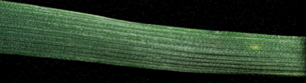
\includegraphics[width=1\textwidth]{Yr15/Figures/population/Yr15Photo.png}
        \label{fig:yr15.yr15Photo}
    \end{subfigure}
    ~
    \begin{subfigure}[b]{0.4\textwidth}
        \caption{}
        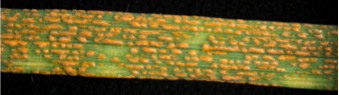
\includegraphics[width=1\textwidth]{Yr15/Figures/population/AVSPhoto.png}
        \label{fig:yr15:avsPhoto}
    \end{subfigure}

     \begin{subfigure}[b]{0.9\textwidth}
     \caption{}
        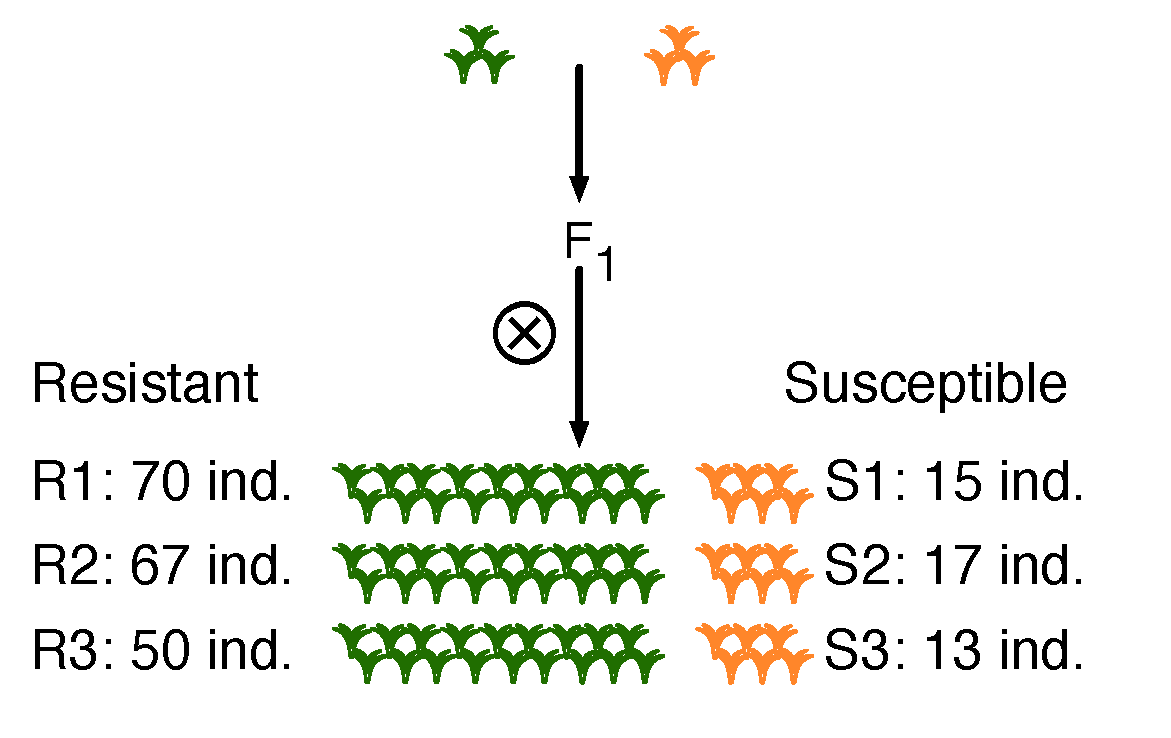
\includegraphics[width=1\textwidth]{Yr15/Figures/population/F2Population.pdf} 
    \label{fig:yr15:f2}
  \end{subfigure}

    \caption[Avocet + \textit{Yr15} $F_{2}$  mapping population.]{Avocet + \textit{Yr15} $F_{2}$  mapping population. Response of (\subref{fig:yr15.yr15Photo}) Avocet + \textit{Yr15} and (\subref{fig:yr15:avsPhoto}) Avocet when inoculated with \textit{Puccinia striiformis} f. sp.  \textit{tritici} at the three leaf stage. (\subref{fig:yr15:f2}) The phenotype of the $F_{2}$ population was used to produce 6 bulks, 3 resistant and 2 susceptible. The RNA was pooled in bulks accordingly. Adapted from \citep{Ramirez-Gonzalez2015b}}

%\end{wrapfigure}
\end{figure}
%\end{SCfigure}


\section{Sequencing and mapping.} 

RNA-Seq was used as a reduced representation method, and thus avoided sequencing the non-coding regions.
This effectively reduces the search space, which is especially important in a species with a genome as rich in repeat content as wheat.
The sequencing of the bulks and the parents was done on a single Illumina Hi-Seq2000.
The bulks were multiplexed and sequenced on a third of a lane each, as shown on Table \ref{tab:yr15:reads}. 
To ensure that quality of sequencing, \verb|fastqc-0.10| \citep{fastqc}  was run with its default parameters for each of the FASTQ files.  
The GC content was around 52\% in all the samples (Appendix \ref{App:AppendixQCGC}), which is as expected as the sample should be of coding regions, and for wheat the reported GC content in genes is around 55\%.  
The quality of the reads is fairly consistent, in general dropping after base 80 across samples (Appendix \ref{App:AppendixQCRead}). 
\label{yr15:sequencing}

\begin{table}
\centering
\caption{Arrangement and number of sequenced base pairs per sample. }
\label{tab:yr15:reads}
\begin{tabular}{rrccccc}
\toprule
Library & name & Bar code & Lane   &  Reads (\e{8} bp)\\ 
\midrule
LIB1715 & Bulk R1 & ATCACG & 1  & 0.77\\
LIB1716 & Bulk R2 & TAGCTT & 1    & 1.20\\
LIB1717 & Bulk R3 & ACTTGA & 2  & 0.96  \\ 
LIB1718 & Bulk S1 & GGCTAC & 2  & 1.64   \\ 
LIB1719 & Bulk S2 & CGTACG & 2  & 1.49  \\ 
LIB1720 & Bulk S3 & GTGGCC & 1  &1.88  \\ 
LIB1721 & AvocetS & N/A & 3     & 4.13 \\ 
LIB1722 & AvocetS + \textit{Yr15} & N/A & 4   & 3.99  \\ 
\bottomrule
\end{tabular}
\end{table}



%!TEX root = ../../Main.tex
\begin{sidewaystable}
\centering
\caption{Number of genes with a coverage over 20x, 10x and at least one read (\ensuremath{>}0x). }
\label{app:seqAlnCov}
\begin{localsize}{10}{11}

\begin{tabular}{llrrrrrr|rrrr|rr}
\toprule
          &             & \multicolumn{6}{c}{Bulks} & \multicolumn{4}{c}{Bulk  mixes} & \multicolumn{2}{c}{Progenitors}        \\
 Coverage & Reference   & R1     & R2     & R3     & S1     & S2     & S3     & R1+R2       & S1+S2  & R1+R2+R3 & S1+S2+S3 & \textit{Yr15}        & AVS     \\
 \midrule
 20x      & UCW         & 16,434 & 27,871 & 27,223 & 32,287 & 28,669 & 34,898 & 33,968      & 41,019 & 40,985   & 47,507   & 36,808      & 42,248  \\
          &             & 17\%    & 30\%    & 29\%    & 34\%    & 30\%    & 37\%    & 36\%         & 44\%    & 44\%      & 50\%      & 39\%         & 45\%     \\
          & UniGene v60 & 9,643  & 16,182 & 15,222 & 19,549 & 17,397 & 20,567 & 20,219      & 25,270 & 24,598   & 29,052   & 22,107      & 25,842  \\
          &             & 17\%    & 28\%    & 27\%    & 34\%    & 31\%    & 36\%    & 36\%         & 44\%    & 43\%      & 51\%      & 39\%         & 45\%     \\
 \midrule
 10x      & UCW         & 27,371 & 38,282 & 37,777 & 42,658 & 38,999 & 44,610 & 43,266      & 49,473 & 49,182   & 54,781   & 46,356      & 50,760  \\
          &             & 29\%    & 41\%    & 40\%    & 45\%    & 41\%    & 47\%    & 46\%         & 53\%    & 52\%      & 58\%      & 49\%         & 54\%     \\
          & UniGene v60 & 16,201 & 22,948 & 22,130 & 26,200 & 24,130 & 26,914 & 26,318      & 30,579 & 29,857   & 33,557   & 28,044      & 31,095  \\
          &             & 28\%    & 40\%    & 39\%    & 46\%    & 42\%    & 47\%    & 46\%         & 54\%    & 52\%      & 59\%      & 49\%         & 55\%     \\
 \midrule
 \ensuremath{>}0x      & UCW         & 68,302 & 72,484 & 72,957 & 74,694 & 73,290 & 75,201 & 74,397      & 77,093 & 76,715   & 78,796   & 76,275      & 77,080  \\
          &             & 73\%    & 77\%    & 77\%    & 79\%    & 78\%    & 80\%    & 79\%         & 82\%    & 81\%      & 84\%      & 81\%         & 82\%     \\
          & UniGene v60 & 40,717 & 42,489 & 42,595 & 43,625 & 43,059 & 43,748 & 43,393      & 44,655 & 44,364   & 45,392   & 43,732      & 44,596" \\
          &             & 71\%    & 75\%    & 75\%    & 77\%    & 76\%    & 77\%    & 76\%         & 78\%    & 78\%      & 80\%      & 77\%         & 78\%     \\
\bottomrule
\end{tabular}

\end{localsize}
\end{sidewaystable}


When the analysis was started, the draft genome and the corresponding annotation had not been released yet, hence gene models were used instead of a genome reference. 
All the samples were aligned to the UniGenes v60 (56,954 genes) and the gene models from UCW \citep{Krasileva2013} using \verb|BWA 0.5.9| \citep{Li2009}. 
The alignment showed that few genes were very highly expressed, however, there was still sufficient coverage of over 20x in \gls{yr15} across 22,107 and 36,808 genes, on the UniGenes and the UCW gene set, respectively. 
Both gene sets performed similarly in terms of the percentage of genes with reads and percentage of aligned reads. 
The percentage of genes with a coverage of at least $20x$ is $45\%$ and $39\%$ for \gls{avs} and \gls{yr15}, irrespective of the reference gene set chosen (Figure \ref{fig:yr15:covPerGene}).
Since each individual bulk has a lower coverage, the susceptible and resistant reads were merged \textit{in silico} as: (i) susceptible bulks 1 with 2 (S1+S2) and resistant bulks 1 with 2 (R1+R2) and (ii) all the susceptible (S1+S2+S3) and resistant bulks (R1+R2+R3). 
The merged samples increased the percentage of genes with coverage over 20x  to 44\% and 50\% in the resistant and susceptible bulks (Table \ref{app:seqAlnCov}), which is close to the coverage from the progenitors.
We treated bulk 3 slightly differently since these bulks included a few lines which were borderline with respect to their phenotype. 
Therefore exclusion of bulk 3 plants in the S1+S2 and R1+R2 bulk would provide the "cleanest" possible data, whereas inclusion in the second set of bulks would allow us to evaluate the effect of possible noise within the system. 

\begin{figure}
\centering
\begin{subfigure}{0.38\textwidth}
    \caption{}
     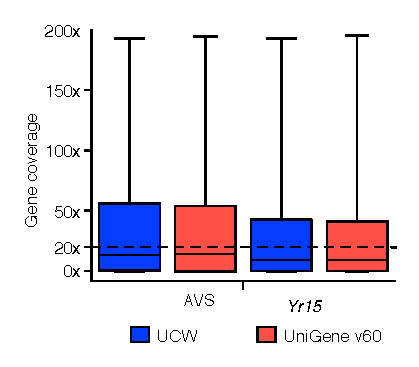
\includegraphics[width=1\textwidth]{Yr15/Figures/CoveragePerGene.pdf} 
    \label{fig:yr15:covPerGene}
\end{subfigure}
~
\begin{subfigure}{0.58\textwidth}
    \caption{}
    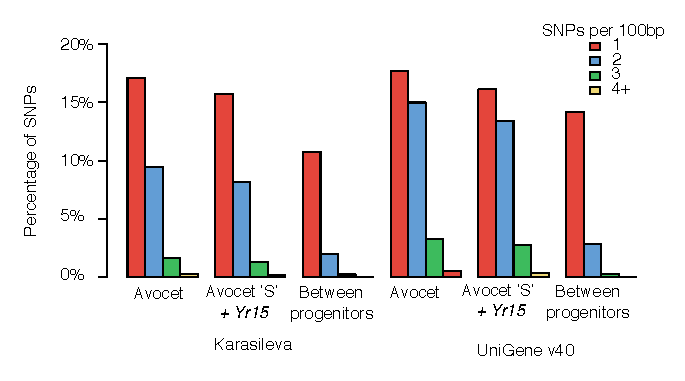
\includegraphics[width=1\textwidth]{Yr15/Figures/PercentageOfSnps.pdf} 
    
    \label{fig:yr15:SNPper}
\end{subfigure}
\caption[Coverage and SNPs between progenitors]{Coverage and SNPs between progenitors. (\subref{fig:yr15:covPerGene}) Box plot distribution of the gene coverage of the parent reads (\gls{avs} and \gls{yr15}) across the \acrshort{ucw} (blue) and the UniGene (red) gene models. The dashed line represents the 20x minimum coverage required for SNP calling. The full line represents the average coverage across all gene models. (\subref{fig:yr15:SNPper}) Percentage of genes exhibiting SNPs across references. The number of \gls{snp}s between the parent reads and the corresponding references was calculated (per 100 bp, rounded). The ‘between-parents’ category corresponds to putative SNPs when comparing the consensus sequence between \gls{avs} and \gls{yr15} Adapted from \citet{Ramirez-Gonzalez2015b} }
\end{figure}



\section{SNP Calling}
\label{yr15:snpCalling}

The \gls{snp} calling was done on positions with a coverage of at least $20x$ on the progenitor lines against the gene reference. The \gls{avs} progenitor had roughly $3\%$ more genes with polymorphisms than \gls{yr15}, consistent with the difference in coverage, suggesting that with a higher coverage we could recover more \gls{snp}s from \gls{yr15}.
The UniGenes have a higher number of \gls{snp}s because the \gls{ucw} gene models have a higher number of monomorphic genes when compared to the UniGenes (Figure \ref{fig:yr15:SNPper}; Table \ref{app:yr15:cntSNP100bp}). 
The difference in the number of relative monomorphic SNPs between reference can be explained by the fact that in the UniGenes set many homeologoues might have been collapsed into a single representative sequence, whereas the \acrshort{ucw} gene set is homoeologue-specific.
Therefore, mapping to the correct homeologue is improved in the \acrshort{ucw} gene set over the UniGenes.


%!TEX root = ../../Main.tex
\begin{table}
\caption{ Count of SNPs per 100 bp on genes with at least 20x coverage. }
\centering
\label{app:yr15:cntSNP100bp}
\begin{localsize}{10}{12}
\begin{tabular}{lrrrrrrr}
\toprule
 SNPs  & \multicolumn{3}{c}{UCW}  &  &  \multicolumn{3}{c}{UniGene v60 }                                 \\
 \cline{2-4}
 \cline{6-8}
\pbox{1cm}{per 100bp}         & AVS   & \pbox{1.5cm}{\centering AVS+ \textit{Yr15}} & \pbox{1.8cm}{\centering Between progenitors} &      & AVS         & \pbox{1.5cm}{\centering AVS+ \textit{Yr15}} & \pbox{1.8cm}{\centering Between progenitors} \\
\midrule
 0               & 67, 389       & 70,338 & 81,921             &      & 36,210       & 38,339      & 47,097               \\
                 & 71.6\% & 74.7\%      & 87.0\%               &      & 63.6\%       & 67.3\%      & 82.7\%               \\
 \midrule
 1               & 16,111 & 14,770      & 10,107               &      & 10,058       & 9,175       & 8,061                \\
                 & 17.1\% & 15.7\%      & 10.7\%               &      & 17.7\%       & 16.1\%      & 14.2\%               \\
 \midrule
 2               & 8,904  & 7,676       & 1,893                &      & 8,529	         & 7,648       & 1,621                \\
                 & 9.5\%  & 8.2\%       & 2.0\%                &      & 15.0\%       & 13.4\%      & 2.9\%                \\
 \midrule
 3               & 1,517  & 1,192       & 215                  &      & 1,870        & 1,568       & 59       \\
                 & 1.6\%  & 1.3\%       & 0.2\%                &      & 3.3\%        & 2.8\%       & 0.3\%                \\
 \midrule
 4+              & 253    & 198         & 38                   &      & 287          & 224         & 16                  \\
                 & 0.3\%  & 0.2\%       & 0.0\%                &      & 0.5\%        & 0.4\%       & 0.0\%                \\
\bottomrule
\end{tabular}
\end{localsize}
\end{table}


Both gene sets were derived from varieties different to \gls{avs} and are likely to be incomplete, hence we set a low threshold of at least 20\% of the observed nucleotides on any position to call a \gls{snp}. 
To represent cases where more than one consensus base is called we use \gls{iuapc} codes (\citet{Cornish-Bowden1985}; Section \ref{lit:ambiguity}; Figure \ref{fig:yr15:bfr}).  
To focus the analysis on informative \gls{snp}s, the common varietal SNPs and variations between homoeologues were removed by finding cases where the consensus call on both progenitors was the same. 
The \gls{snp}s that are unique to a single parental were examined in detail. 
There are 66,426 putative SNPs across 16,022 (17\%) \gls{ucw} genes and 52,262 \acrshortpl{snp} on 11,056 UniGenes (19.4\%; Figure \ref{fig:yr15:geneCount}).  

\begin{SCfigure}
    %\centering
    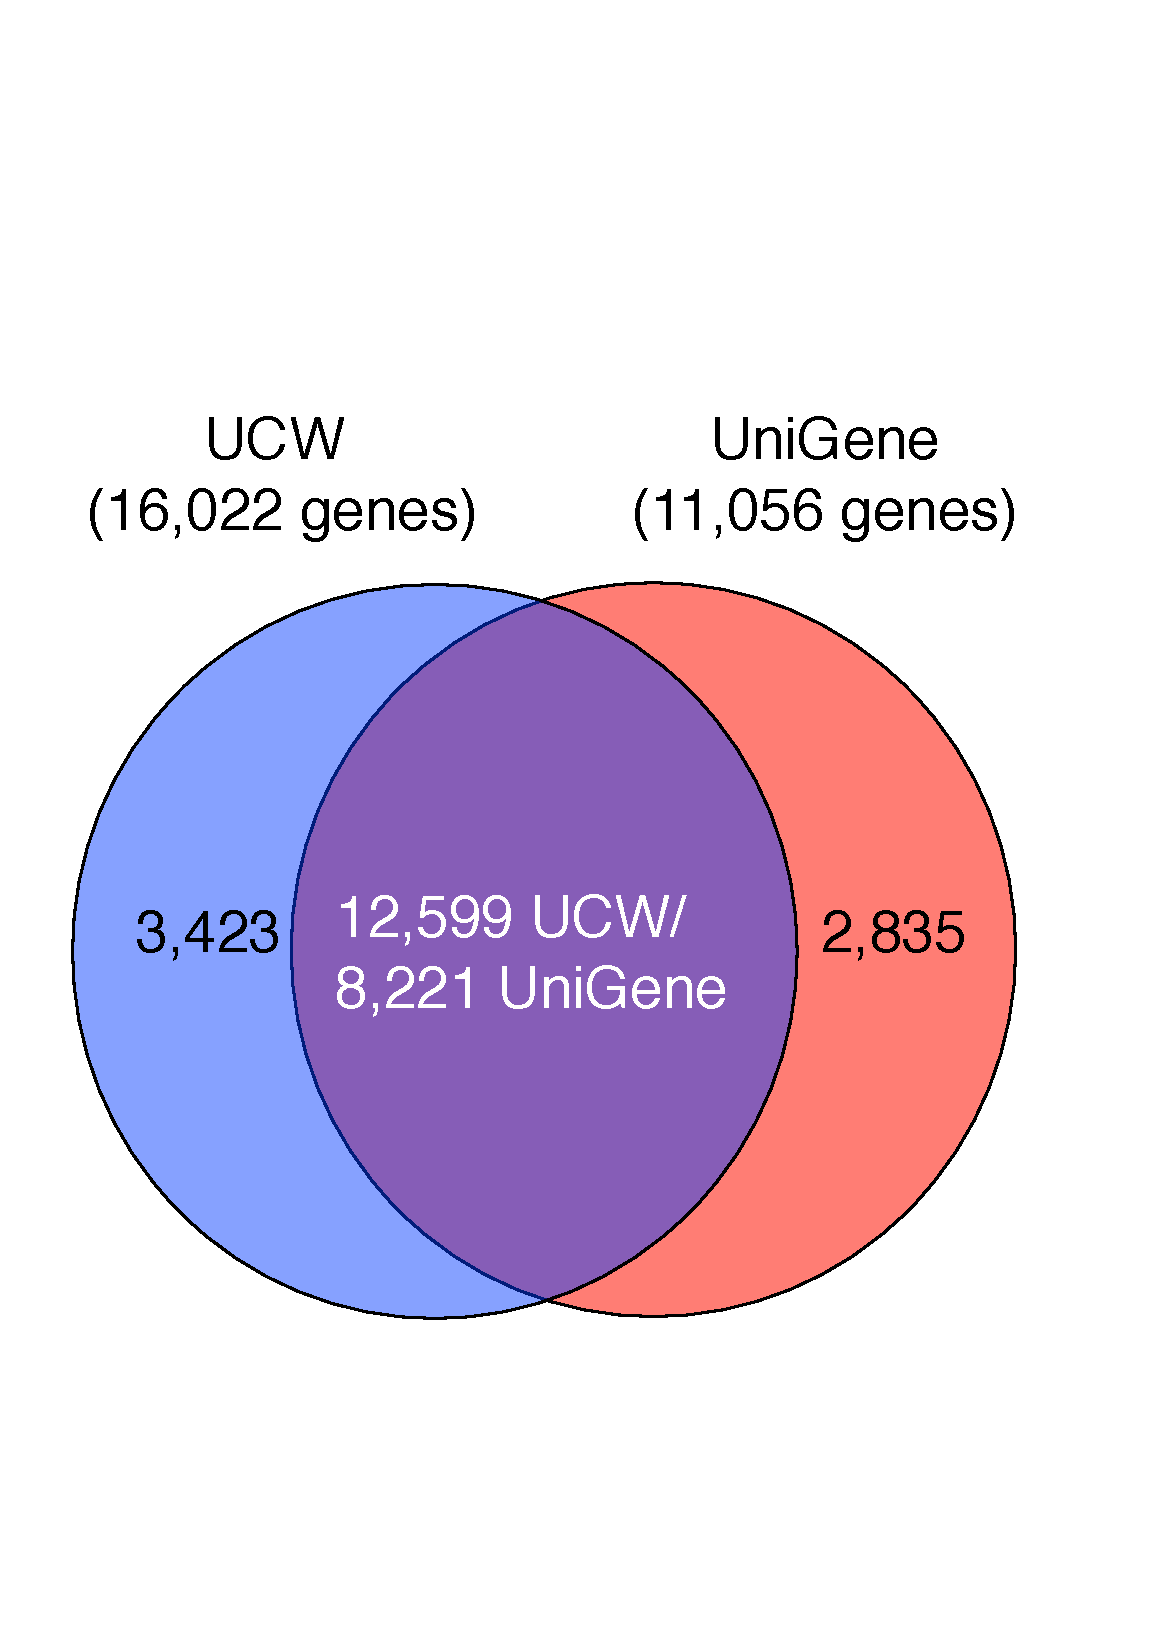
\includegraphics[width=0.4\textwidth]{Yr15/Figures/geneCounts.pdf} 
    \caption[Gene models with putative SNPs]{Gene models with putative SNPs in common between the UCW and UniGenes reference. The intersection represents the genes that are common in both sets. Adapted from \citet{Ramirez-Gonzalez2015b}}
    \label{fig:yr15:geneCount}
\end{SCfigure}

%!TEX root = ../../Main.tex
\begin{table}
\centering
\caption{ Number of genes assigned to the wheat chromosome arm CSS scaffolds \citep{Mayer2014} using the best hit from BLAT \citep{Kent2002} }
\label{tab:yr15:genesToCSS}
\begin{localsize}{10}{12}
\begin{tabular}{lrrr}
\toprule
 \pbox{2.2cm}{Wheat \\Chromosome Arm}    & UCW (94,177)    & UniGene v60 (56,954)   & Total (151,131)   \\
\midrule
 1AL                     & 3,251 (3.45\%)   & 1,404 (2.47\%)          & 4,655 (3.08\%)     \\
 1AS                     & 1,366 (1.45\%)   & 560 (0.98\%)            & 1,926 (1.27\%)     \\
 1BL                     & 2,610 (2.77\%)   & 1,280 (2.25\%)          & 3,890 (2.57\%)     \\
 1BS                     & 1,487 (1.58\%)   & 693 (1.22\%)            & 2,180 (1.44\%)     \\
 1DL                     & 997 (1.06\%)     & 1,057 (1.86\%)          & 2,054 (1.36\%)     \\
 1DS                     & 753 (0.80\%)     & 687 (1.21\%)            & 1,440 (0.95\%)     \\
 \midrule
 2AL                     & 3,491 (3.71\%)   & 1,460 (2.56\%)          & 4,951 (3.28\%)     \\
 2AS                     & 2,305 (2.45\%)   & 974 (1.71\%)            & 3,279 (2.17\%)     \\
 2BL                     & 3,658 (3.88\%)   & 1,546 (2.71\%)          & 5,204 (3.44\%)     \\
 2BS                     & 2,790 (2.96\%)   & 1,139 (2.00\%)          & 3,929 (2.60\%)     \\
 2DL                     & 1,098 (1.17\%)   & 1,069 (1.88\%)          & 2,167 (1.43\%)     \\
 2DS                     & 796 (0.85\%)     & 833 (1.46\%)            & 1,629 (1.08\%)     \\
 \midrule
 3AL                     & 2,135 (2.27\%)   & 978 (1.72\%)            & 3,113 (2.06\%)     \\
 3AS                     & 1,543 (1.64\%)   & 718 (1.26\%)            & 2,261 (1.50\%)     \\
 3B                      & 6,559 (6.96\%)   & 2,839 (4.98\%)          & 9,398 (6.22\%)     \\
 3DL                     & 915 (0.97\%)     & 938 (1.65\%)            & 1,853 (1.23\%)     \\
 3DS                     & 412 (0.44\%)     & 450 (0.79\%)            & 862 (0.57\%)       \\
 \midrule
 4AL                     & 3,393 (3.60\%)   & 1,335 (2.34\%)          & 4,728 (3.13\%)     \\
 4AS                     & 2,011 (2.14\%)   & 817 (1.43\%)            & 2,828 (1.87\%)     \\
 4BL                     & 2,119 (2.25\%)   & 898 (1.58\%)            & 3,017 (2.00\%)     \\
 4BS                     & 1,946 (2.07\%)   & 892 (1.57\%)            & 2,838 (1.88\%)     \\
 4DL                     & 1,069 (1.14\%)   & 945 (1.66\%)            & 2,014 (1.33\%)     \\
 4DS                     & 800 (0.85\%)     & 699 (1.23\%)            & 1,499 (0.99\%)     \\
 \midrule
 5AL                     & 2,640 (2.80\%)   & 1,132 (1.99\%)          & 3,772 (2.50\%)     \\
 5AS                     & 963 (1.02\%)     & 407 (0.71\%)            & 1,370 (0.91\%)     \\
 5BL                     & 5,324 (5.65\%)   & 1,943 (3.41\%)          & 7,267 (4.81\%)     \\
 5BS                     & 1,360 (1.44\%)   & 591 (1.04\%)            & 1,951 (1.29\%)     \\
 5DL                     & 2,067 (2.19\%)   & 1,688 (2.96\%)          & 3,755 (2.48\%)     \\
 5DS                     & 620 (0.66\%)     & 614 (1.08\%)            & 1,234 (0.82\%)     \\
 \midrule
 6AL                     & 2,397 (2.55\%)   & 896 (1.57\%)            & 3,293 (2.18\%)     \\
 6AS                     & 2,285 (2.43\%)   & 936 (1.64\%)            & 3,221 (2.13\%)     \\
 6BL                     & 1,564 (1.66\%)   & 820 (1.44\%)            & 2,384 (1.58\%)     \\
 6BS                     & 1,308 (1.39\%)   & 731 (1.28\%)            & 2,039 (1.35\%)     \\
 6DL                     & 1,399 (1.49\%)   & 1,050 (1.84\%)          & 2,449 (1.62\%)     \\
 6DS                     & 870 (0.92\%)     & 680 (1.19\%)            & 1,550 (1.03\%)     \\
 \midrule
 7AL                     & 1,918 (2.04\%)   & 849 (1.49\%)            & 2,767 (1.83\%)     \\
 7AS                     & 1,717 (1.82\%)   & 764 (1.34\%)            & 2,481 (1.64\%)     \\
 7BL                     & 1,592 (1.69\%)   & 776 (1.36\%)            & 2,368 (1.57\%)     \\
 7BS                     & 1,239 (1.32\%)   & 713 (1.25\%)            & 1,952 (1.29\%)     \\
 7DL                     & 2,040 (2.17\%)   & 1,301 (2.28\%)          & 3,341 (2.21\%)     \\
 7DS                     & 1,224 (1.30\%)   & 1,016 (1.78\%)          & 2,240 (1.48\%)     \\
 \midrule
 Assigned                & 80,031 (84.98\%) & 41,118 (72.20\%)        & 121,149 (80.16\%)  \\
\bottomrule
\end{tabular}
\end{localsize}
\end{table}

The high number of genes with \gls{snp}s was unexpected as a \gls{bc}6 \gls{nil} used for a $F_2$ mapping population expects to have less than $1\%$ of the genetic background segregating. 
Both sets of gene models were aligned with BLAT \citep{Kent2002} to the \gls{css} assembly \citep{Mayer2014}; the alignment resulted on 80,031 (85.0\%) \acrshort{ucw} gene models and 41,118 (72.2\%) UniGenes assigned to a chromosome arm (Table \ref{tab:yr15:genesToCSS}). 
The SNPs found in the mapped genes are evenly distributed across all the chromosomes (see Section \ref{sub:yr15:inSilico}), suggesting that the \gls{avs} (\gls{jic}, UK) used as parent in the $F_{2}$ is different to the \gls{avs} used for the \acrshort{yr15} \acrshort{nil} development (University of Sydney, Australia).  

To confirm that the \gls{avs} seed stocks from \gls{jic} are distinct to the stocks in Sydney, DNA from both stocks was procured and compared with the iSelect 90k wheat SNP chip. 
Between two independent \gls{avs} seeds from \gls{jic} only 58 out of 71,972 (0.08\%) valid assays were polymorphic. 
Nonetheless, there are over 5,000 ($>7.5\%$) assays with polymorphisms between  \gls{jic}-\gls{avs} and \gls{avs} from Sydney. 
The difference was not expected originally, but considering that the \gls{avs} seeds are coming from different stocks and the fact that in both countries commercial varieties with the same name had been released, it is not surprising. 


\section{Bulk Frequency Ratios}
\label{sec:yr15:bfr}

%!TEX root = ../../Main.tex
\begin{table}
\caption{Total number of SNPs scored in parents, individual bulks and in silico merged bulks. }
\centering
\label{app:yr15:scoredSNPs}
\begin{localsize}{10}{12}
\begin{tabular}{lrrrrrr}
\toprule
 Gene set    & $\frac{R1}{S1}$  & $\frac{R2}{S2}$   & $\frac{R3}{S3}$   & $\frac{R1+R2}{S1+S2}$    & $\frac{R1+R2+R3}{S1+S2+S3}$   & \pbox{1.8cm}{\centering SNPs in  parents}   \\
\midrule
 UCW         & 16,269  & 29,703  & 31,891  & 44,224         & 64,522               & 66,426            \\
             & 24.49\%  & 44.72\%  & 48.01\%  & 66.58\%         & 97.13\%               &                   \\
\midrule
 UniGene v60 & 15,261  & 25,143  & 24,548  & 35,698         & 49,738               & 52,262            \\
             & 29.20\%  & 48.11\%  & 46.97\%  & 68.31\%         & 95.17\%               &                   \\
\bottomrule
\end{tabular}
\end{localsize}
\end{table}

The objective was to find the SNPs enriched (or depleted) in each bulk and hence linked to the phenotype.  \Glspl{snp} originating from \gls{yr15} would be expected to be linked to resistance whereas those from \acrshort{avs} to susceptibility in the segregating population. 
Across individual bulks, it was possible to score between 15,261 (24.5\%) and 31,891(48.0\%) \glspl{snp}s across both reference sets.
On the \textit{in silico} mixes, over $95\%$ of SNPs where scored (Table \ref{app:yr15:scoredSNPs}), suggesting that the coverage of individual bulks is not enough to score all the SNPs.
The scoring was done with the \acrlong{bfr} (\citealt{Trick2012};Figure \ref{fig:yr15:bfr}; Section \ref{yr15:sub:bfr}), which has a value that increases as the \acrshort{yr15} allele is observed more times relatively to the \acrshort{avs} allele.

%!TEX root = ../../Main.tex
\begin{sidewaystable}
\caption{ SNPs in chromosome group 1S vs total number of SNPs with a minimum BFR from 0 to 10. AVS: SNPs coming from \acrlong{avs}. \textit{Yr15}: SNPs comming from \acrlong{yr15}. }
\centering
\label{app:yr15:bfrThresholds}
\begin{localsize}{6}{7}

\begin{tabular}{llp{1cm}p{1cm}p{1cm}p{1cm}p{1cm}p{1cm}p{1cm}p{1cm}p{1cm}p{1cm}}
\toprule
 Min  BFR   & Gene Set    & R1/S1 \textit{Yr15}        & R1/S1 AVS         & R2/S2 \textit{Yr15}         & R2/S2 AVS          & R3/S3 \textit{Yr15}         & R3/S3 AVS          & S1+2/ R1+2 \textit{Yr15}    & S1+2/ R1+2 AVS     & S1+S2+S3/ R1+R2+R3 \textit{Yr15}   & S1+S2+S3/ R1+R2+R3 AVS   \\
\midrule
 0          & UCW         & 308/8,049 (3.83\%) & 305/8,220 (3.71\%) & 505/14,121 (3.58\%) & 556/15,582 (3.57\%) & 532/14,875 (3.58\%) & 623/17,016 (3.66\%) & 670/18,760 (3.57\%) & 885/25,464 (3.48\%) & 860/24,026 (3.58\%)        & 1,505/40,496 (3.72\%)     \\
            & UniGene v60 & 307/7,823 (3.92\%) & 299/7,438 (4.02\%) & 428/12,409 (3.45\%) & 421/12,734 (3.31\%) & 427/12,050 (3.54\%) & 415/12,498 (3.32\%) & 536/15,672 (3.42\%) & 595/20,026 (2.97\%) & 712/19,358 (3.68\%)        & 901/30,380 (2.97\%)       \\
 \midrule
 1          & UCW         & 214/4,415 (4.85\%) & 194/4,108 (4.72\%) & 325/7,603 (4.27\%)  & 314/7,374 (4.26\%)  & 365/7,920 (4.61\%)  & 415/8,850 (4.69\%)  & 426/10,122 (4.21\%) & 494/12,185 (4.05\%) & 539/13,037 (4.13\%)        & 842/19,466 (4.33\%)       \\
            & UniGene v60 & 207/4,474 (4.63\%) & 194/3,630 (5.34\%) & 269/6,649 (4.05\%)  & 269/6,193 (4.34\%)  & 279/6,511 (4.29\%)  & 272/6,436 (4.23\%)  & 329/8,704 (3.78\%)  & 369/9,343 (3.95\%)  & 446/10,860 (4.11\%)        & 541/14,226 (3.80\%)       \\
 \midrule
 2          & UCW         & 92/651 (14.13\%)   & 75/671 (11.18\%)   & 142/1,372 (10.35\%) & 111/1,101 (10.08\%) & 147/1,162 (12.65\%) & 149/1,411 (10.56\%) & 167/1,324 (12.61\%) & 163/1,478 (11.03\%) & 194/1,370 (14.16\%)        & 207/1,765 (11.73\%)       \\
            & UniGene v60 & 77/568 (13.56\%)   & 58/527 (11.01\%)   & 101/1,017 (9.93\%)  & 81/720 (11.25\%)    & 105/775 (13.55\%)   & 84/867 (9.69\%)     & 122/991 (12.31\%)   & 116/973 (11.92\%)   & 145/1,030 (14.08\%)        & 132/1,210 (10.91\%)       \\
 \midrule
 3          & UCW         & 78/299 (26.09\%)   & 45/295 (15.25\%)   & 118/646 (18.27\%)   & 70/409 (17.11\%)    & 123/577 (21.32\%)   & 85/494 (17.21\%)    & 145/673 (21.55\%)   & 98/563 (17.41\%)    & 168/768 (21.88\%)          & 122/665 (18.35\%)         \\
            & UniGene v60 & 65/254 (25.59\%)   & 26/186 (13.98\%)   & 87/499 (17.43\%)    & 54/294 (18.37\%)    & 93/379 (24.54\%)    & 48/315 (15.24\%)    & 107/525 (20.38\%)   & 66/379 (17.41\%)    & 133/617 (21.56\%)          & 78/489 (15.95\%)          \\
 \midrule
 4          & UCW         & 75/232 (32.33\%)   & 28/160 (17.50\%)   & 109/484 (22.52\%)   & 44/217 (20.28\%)    & 105/416 (25.24\%)   & 44/246 (17.89\%)    & 134/539 (24.86\%)   & 53/277 (19.13\%)    & 149/640 (23.28\%)          & 64/323 (19.81\%)          \\
            & UniGene v60 & 63/192 (32.81\%)   & 17/104 (16.35\%)   & 83/390 (21.28\%)    & 29/155 (18.71\%)    & 82/288 (28.47\%)    & 29/173 (16.76\%)    & 104/431 (24.13\%)   & 40/214 (18.69\%)    & 127/519 (24.47\%)          & 29/266 (10.90\%)          \\
 \midrule
 5          & UCW         & 69/202 (34.16\%)   & 19/108 (17.59\%)   & 95/416 (22.84\%)    & 33/138 (23.91\%)    & 96/354 (27.12\%)    & 23/143 (16.08\%)    & 127/477 (26.62\%)   & 28/175 (16.00\%)    & 140/580 (24.14\%)          & 42/222 (18.92\%)          \\
            & UniGene v60 & 58/163 (35.58\%)   & 11/70 (15.71\%)    & 76/337 (22.55\%)    & 14/102 (13.73\%)    & 70/228 (30.70\%)    & 20/112 (17.86\%)    & 100/389 (25.71\%)   & 23/146 (15.75\%)    & 118/469 (25.16\%)          & 21/178 (11.80\%)          \\
 \midrule
 6          & UCW         & 65/179 (36.31\%)   & 12/85 (14.12\%)    & 86/380 (22.63\%)    & 22/98 (22.45\%)     & 87/299 (29.10\%)    & 11/94 (11.70\%)     & 122/429 (28.44\%)   & 21/130 (16.15\%)    & 126/514 (24.51\%)          & 29/165 (17.58\%)          \\
            & UniGene v60 & 57/151 (37.75\%)   & 7/48 (14.58\%)     & 73/300 (24.33\%)    & 6/71     (8.45\%)   & 65/191 (34.03\%)    & 13/84 (15.48\%)     & 98/358 (27.37\%)    & 20/122 (16.39\%)    & 115/439 (26.20\%)          & 16/143 (11.19\%)          \\
 \midrule
 7          & UCW         & 58/161 (36.02\%)   & 11/73 (15.07\%)    & 77/340 (22.65\%)    & 13/74 (17.57\%)     & 73/248 (29.44\%)    & 7/69 (10.14\%)      & 116/393 (29.52\%)   & 20/111 (18.02\%)    & 114/468 (24.36\%)          & 22/143 (15.38\%)          \\
            & UniGene v60 & 56/132 (42.42\%)   & 4/37 (10.81\%)     & 68/273 (24.91\%)    & 5/58    (8.62\%)    & 60/171 (35.09\%)    & 9/64 (14.06\%)      & 94/334 (28.14\%)    & 18/103 (17.48\%)    & 113/412 (27.43\%)          & 16/124 (12.90\%)          \\
 \midrule
 8          & UCW         & 58/149 (38.93\%)   & 10/62 (16.13\%)    & 68/310 (21.94\%)    & 12/59 (20.34\%)     & 66/214 (30.84\%)    & 6/56 (10.71\%)      & 104/359 (28.97\%)   & 17/102 (16.67\%)    & 108/429 (25.17\%)          & 16/119 (13.45\%)          \\
            & UniGene v60 & 55/126 (43.65\%)   & 3/33    (9.09\%)   & 64/255 (25.10\%)    & 5/50 (10.00\%)      & 55/150 (36.67\%)    & 9/55 (16.36\%)      & 91/313 (29.07\%)    & 14/89 (15.73\%)     & 105/376 (27.93\%)          & 15/108 (13.89\%)          \\
 \midrule
 9          & UCW         & 54/135 (40.00\%)   & 8/53 (15.09\%)     & 63/289 (21.80\%)    & 8/51 (15.69\%)      & 61/182 (33.52\%)    & 5/49 (10.20\%)      & 100/331 (30.21\%)   & 15/91 (16.48\%)     & 100/387 (25.84\%)          & 13/106 (12.26\%)          \\
            & UniGene v60 & 53/117 (45.30\%)   & 1/30    (3.33\%)   & 62/244 (25.41\%)    & 5/46 (10.87\%)      & 50/136 (36.76\%)    & 9/48 (18.75\%)      & 88/291 (30.24\%)    & 13/83 (15.66\%)     & 97/345 (28.12\%)           & 12/99 (12.12\%)           \\
 \midrule
 10         & UCW         & 52/126 (41.27\%)   & 8/50 (16.00\%)     & 62/279 (22.22\%)    & 8/50 (16.00\%)      & 56/165 (33.94\%)    & 4/45    (8.89\%)    & 96/309 (31.07\%)    & 14/82 (17.07\%)     & 91/355 (25.63\%)           & 13/100 (13.00\%)          \\
            & UniGene v60 & 50/105 (47.62\%)   & 1/28    (3.57\%)   & 60/226 (26.55\%)    & 5/39 (12.82\%)      & 43/119 (36.13\%)    & 7/45 (15.56\%)      & 85/272 (31.25\%)    & 13/82 (15.85\%)     & 92/318 (28.93\%)           & 12/97 (12.37\%)           \\
\bottomrule
\end{tabular}
\end{localsize}
\end{sidewaystable}


When increasing the minimum \acrshort{bfr} threshold, enrichment of SNPs was observed in the short arm of the group 1 chromosomes (1S). 
Without taking into account the \acrshort{bfr}, $~3.6\%$ of the SNPs are located in the 1S group, similar to the number of SNPs located in other groups \ref{tab:yr15:genesToCSS}. 
However, when increasing the threshold  (between $BFR > 5 $ and $BFR > 7$) the relative number of SNPs in group 1S increases. 
After $BFR>7$ the gains in relative enrichment only improves marginally, but the number of called SNPs is reduced (Table \ref{app:yr15:bfrThresholds}; Figure \ref{fig:yr15:bfrChange}).
For that reason, SNPs with a $BFR>6$ were selected for further validation. 
The method described by \citet{Trick2012} was extended to include cases where there is a complete lack of coverage in one of the samples ($BFR=\infty$), which is an ideal case where the linkage between the SNP and the phenotype is perfect. 
A total of 1,582 SNPs across 1,173 genes had a $BFR>6$.



\begin{figure}
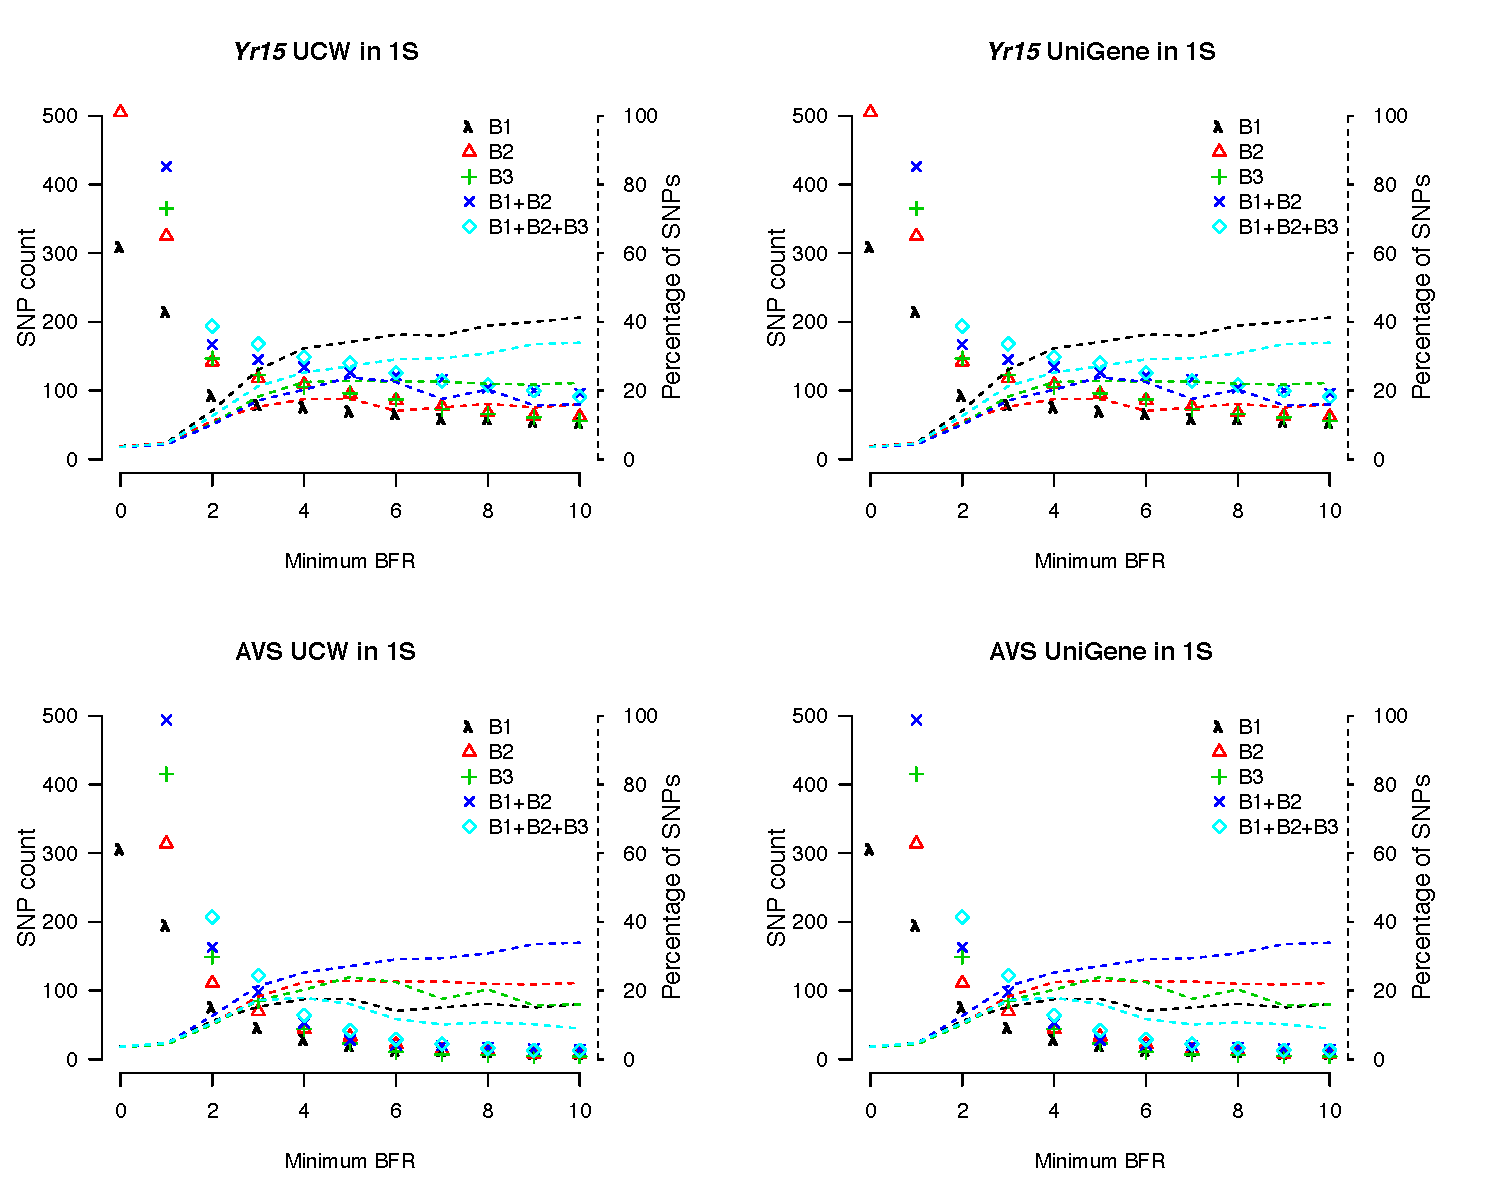
\includegraphics[width=1\textwidth]{Yr15/Figures/bfrChanges.pdf}
\caption[Effect of BFR threshold on the number of SNPs]{Effect of BFR threshold on the number of SNPs across the short arm of chromosome group 1. Figure previously published in \citet{Ramirez-Gonzalez2015b}. }
\label{fig:yr15:bfrChange}
\end{figure}

\section{\textit{In silico} mapping}
\label{sub:yr15:inSilico}
From the mapped SNPs with a $BFR>6$, 872 of 1,582 ($\sim60\%$) were assigned to the chromosomes in group 1 of hexaploid wheat, being the only group with more than $4\%$ of the SNPs assigned to it (Table \ref{app:yr15:bfr6Mapping}). 
From group 1, the B genome contained the higher proportion of SNPs mapped ($54\%$), having 255 ($54\%$) and 214 ($46\%$) assigned to the long and short arms respectively (Figure \ref{fig:yr15:snpsBFR6Group1}).  
These results are expected since previous studies have located \acrshort{yr15} near the centromere in the short arm of chromosome 1B and the \acrshort{yr15} introgression contains regions from the long and short arm from \textit{T. diccocoides} \citep{Murphy2009,Peng2000,Grama1997}. 

\begin{SCfigure}
  \centering
    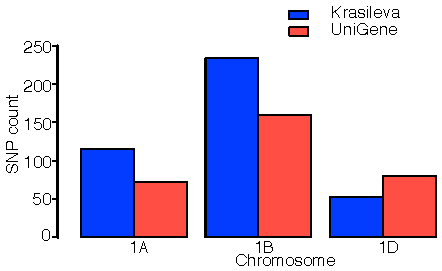
\includegraphics[width=0.5\textwidth]{Yr15/Figures/mapping/snpsBFR6Group1.pdf}
  \caption[Location of SNPs with BFR\textgreater6.]{Location of SNPs with $BFR>6$ according to the best alignment of the UniGene (red) and UCW (blue) gene models to the flow-sorted group 1 chromosomes from the \gls{css} \citep{Mayer2014}. Figure adapted from \citet{Ramirez-Gonzalez2015b}.} 
  \label{fig:yr15:snpsBFR6Group1}
\end{SCfigure}

%!TEX root = ../../Main.tex
\begin{sidewaystable}
\caption{ SNP and genes with BFR > 6 mapping to each of the chromosomes from the CSS assemblies. The chromosome assignment on the "Genetically mapped" column correspond to the map published in \citet{Wang2014}). }
\centering
\label{app:yr15:bfr6Mapping}
\begin{localsize}{6}{9}

\begin{tabular}{rrrrrrrrrrrrrrrrrrrr}
\toprule
Reference & \multicolumn{9}{c}{CSS assemblies}        &    & \multicolumn{9}{c}{Genetically mapped}   \\
 \cline{2-10}
 \cline{12-20}
Chromosome & \multicolumn{4}{c}{UCW gene models} &    & \multicolumn{4}{c}{UniGene v60}&    & \multicolumn{4}{c}{UCW gene models} &    & \multicolumn{4}{c}{UniGene v60}        \\

 \cline{2-5}
 \cline{7-10}
  \cline{12-15}
 \cline{17-20}
 %\midrule
  arm & 
 \multicolumn{2}{c}{SNPs } & 
 \multicolumn{2}{c}{Genes } &  &
 \multicolumn{2}{c}{SNPs } & 
 \multicolumn{2}{c}{Genes } &     &  
 \multicolumn{2}{c}{SNPs } & 
 \multicolumn{2}{c}{Genes } & &
 \multicolumn{2}{c}{SNPs } & 
 \multicolumn{2}{c}{Genes }      
 \\
 \midrule
 1AL            & 113                   & 13.15\% & 79    & 12.29\% &    & 78          & 10.79\% & 50    & 9.43\%  &    & 14                     & 1.63\%  & 8     & 1.24\%  &    & 7           & 0.97\%  & 4     & 0.75\%  \\
 1AS            & 26                    & 3.03\%  & 21    & 3.27\%  &    & 20          & 2.77\%  & 17    & 3.21\%  &    & 42                     & 4.89\%  & 32    & 4.98\%  &    & 38          & 5.26\%  & 28    & 5.28\%  \\
 1BL            & 157                   & 18.28\% & 110   & 17.11\% &    & 98          & 13.55\% & 64    & 12.08\% &    & 60                     & 6.98\%  & 35    & 5.44\%  &    & 36          & 4.98\%  & 23    & 4.34\%  \\
 1BS            & 120                   & 13.97\% & 74    & 11.51\% &    & 94          & 13.00\% & 44    & 8.30\%  &    & 127                    & 14.78\% & 80    & 12.44\% &    & 102         & 14.11\% & 46    & 8.68\%  \\
 1DL            & 30                    & 3.49\%  & 21    & 3.27\%  &    & 58          & 8.02\%  & 47    & 8.87\%  &    & 2                      & 0.23\%  & 2     & 0.31\%  &    & 4           & 0.55\%  & 4     & 0.75\%  \\
 1DS            & 40                    & 4.66\%  & 25    & 3.89\%  &    & 38          & 5.26\%  & 24    & 4.53\%  &    & 12                     & 1.40\%  & 6     & 0.93\%  &    & 8           & 1.11\%  & 5     & 0.94\%  \\
  \midrule
 2AL            & 22                    & 2.56\%  & 20    & 3.11\%  &    & 14          & 1.94\%  & 12    & 2.26\%  &    & 9                      & 1.05\%  & 8     & 1.24\%  &    & 7           & 0.97\%  & 5     & 0.94\%  \\
 2AS            & 11                    & 1.28\%  & 11    & 1.71\%  &    & 10          & 1.38\%  & 7     & 1.32\%  &    & 9                      & 1.05\%  & 9     & 1.40\%  &    & 2           & 0.28\%  & 2     & 0.38\%  \\
 2BL            & 17                    & 1.98\%  & 15    & 2.33\%  &    & 18          & 2.49\%  & 17    & 3.21\%  &    & 7                      & 0.81\%  & 5     & 0.78\%  &    & 4           & 0.55\%  & 4     & 0.75\%  \\
 2BS            & 11                    & 1.28\%  & 10    & 1.56\%  &    & 12          & 1.66\%  & 7     & 1.32\%  &    & 13                     & 1.51\%  & 12    & 1.87\%  &    & 7           & 0.97\%  & 7     & 1.32\%  \\
 2DL            & 2                     & 0.23\%  & 2     & 0.31\%  &    & 15          & 2.07\%  & 10    & 1.89\%  &    & 1                      & 0.12\%  & 1     & 0.16\%  &    & 3           & 0.41\%  & 2     & 0.38\%  \\
 2DS            & 0                     & 0.00\%  & 0     & 0.00\%  &    & 5           & 0.69\%  & 3     & 0.57\%  &    & 0                      & 0.00\%  & 0     & 0.00\%  &    & 0           & 0.00\%  & 0     & 0.00\%  \\
  \midrule
  3AL            & 7                     & 0.81\%  & 7     & 1.09\%  &    & 2           & 0.28\%  & 2     & 0.38\%  &    & 2                      & 0.23\%  & 2     & 0.31\%  &    & 1           & 0.14\%  & 1     & 0.19\%  \\
 3AS            & 1                     & 0.12\%  & 1     & 0.16\%  &    & 4           & 0.55\%  & 4     & 0.75\%  &    & 0                      & 0.00\%  & 0     & 0.00\%  &    & 0           & 0.00\%  & 0     & 0.00\%  \\
 3B             & 31                    & 3.61\%  & 26    & 4.04\%  &    & 28          & 3.87\%  & 24    & 4.53\%  &    & 0                      & 0.00\%  & 0     & 0.00\%  &    & 0           & 0.00\%  & 0     & 0.00\%  \\
 3BL            & 0                     & 0.00\%  & 0     & 0.00\%  &    & 0           & 0.00\%  & 0     & 0.00\%  &    & 9                      & 1.05\%  & 7     & 1.09\%  &    & 4           & 0.55\%  & 4     & 0.75\%  \\
 3BS            & 0                     & 0.00\%  & 0     & 0.00\%  &    & 0           & 0.00\%  & 0     & 0.00\%  &    & 2                      & 0.23\%  & 2     & 0.31\%  &    & 5           & 0.69\%  & 5     & 0.94\%  \\
 3DL            & 7                     & 0.81\%  & 6     & 0.93\%  &    & 2           & 0.28\%  & 2     & 0.38\%  &    & 1                      & 0.12\%  & 1     & 0.16\%  &    & 0           & 0.00\%  & 0     & 0.00\%  \\
 3DS            & 1                     & 0.12\%  & 1     & 0.16\%  &    & 2           & 0.28\%  & 2     & 0.38\%  &    & 0                      & 0.00\%  & 0     & 0.00\%  &    & 0           & 0.00\%  & 0     & 0.00\%  \\
  \midrule
  4AL            & 18                    & 2.10\%  & 15    & 2.33\%  &    & 6           & 0.83\%  & 6     & 1.13\%  &    & 14                     & 1.63\%  & 11    & 1.71\%  &    & 5           & 0.69\%  & 4     & 0.75\%  \\
 4AS            & 5                     & 0.58\%  & 5     & 0.78\%  &    & 6           & 0.83\%  & 5     & 0.94\%  &    & 0                      & 0.00\%  & 0     & 0.00\%  &    & 0           & 0.00\%  & 0     & 0.00\%  \\
 4BL            & 11                    & 1.28\%  & 10    & 1.56\%  &    & 6           & 0.83\%  & 6     & 1.13\%  &    & 3                      & 0.35\%  & 3     & 0.47\%  &    & 4           & 0.55\%  & 4     & 0.75\%  \\
 4BS            & 6                     & 0.70\%  & 5     & 0.78\%  &    & 13          & 1.80\%  & 10    & 1.89\%  &    & 4                      & 0.47\%  & 3     & 0.47\%  &    & 4           & 0.55\%  & 3     & 0.57\%  \\
 4DL            & 4                     & 0.47\%  & 4     & 0.62\%  &    & 5           & 0.69\%  & 5     & 0.94\%  &    & 0                      & 0.00\%  & 0     & 0.00\%  &    & 1           & 0.14\%  & 1     & 0.19\%  \\
 4DS            & 2                     & 0.23\%  & 2     & 0.31\%  &    & 5           & 0.69\%  & 4     & 0.75\%  &    & 0                      & 0.00\%  & 0     & 0.00\%  &    & 1           & 0.14\%  & 1     & 0.19\%  \\
  \midrule
  5AL            & 7                     & 0.81\%  & 5     & 0.78\%  &    & 3           & 0.41\%  & 3     & 0.57\%  &    & 3                      & 0.35\%  & 2     & 0.31\%  &    & 1           & 0.14\%  & 1     & 0.19\%  \\
 5AS            & 1                     & 0.12\%  & 1     & 0.16\%  &    & 2           & 0.28\%  & 2     & 0.38\%  &    & 1                      & 0.12\%  & 1     & 0.16\%  &    & 1           & 0.14\%  & 1     & 0.19\%  \\
 5BL            & 31                    & 3.61\%  & 28    & 4.35\%  &    & 14          & 1.94\%  & 14    & 2.64\%  &    & 12                     & 1.40\%  & 12    & 1.87\%  &    & 6           & 0.83\%  & 6     & 1.13\%  \\
 5BS            & 7                     & 0.81\%  & 5     & 0.78\%  &    & 6           & 0.83\%  & 5     & 0.94\%  &    & 2                      & 0.23\%  & 2     & 0.31\%  &    & 1           & 0.14\%  & 1     & 0.19\%  \\
 5DL            & 8                     & 0.93\%  & 7     & 1.09\%  &    & 15          & 2.07\%  & 14    & 2.64\%  &    & 2                      & 0.23\%  & 2     & 0.31\%  &    & 6           & 0.83\%  & 6     & 1.13\%  \\
 5DS            & 4                     & 0.47\%  & 3     & 0.47\%  &    & 6           & 0.83\%  & 5     & 0.94\%  &    & 0                      & 0.00\%  & 0     & 0.00\%  &    & 0           & 0.00\%  & 0     & 0.00\%  \\
  \midrule
  6AL            & 22                    & 2.56\%  & 17    & 2.64\%  &    & 9           & 1.24\%  & 7     & 1.32\%  &    & 6                      & 0.70\%  & 5     & 0.78\%  &    & 3           & 0.41\%  & 3     & 0.57\%  \\
 6AS            & 8                     & 0.93\%  & 8     & 1.24\%  &    & 11          & 1.52\%  & 10    & 1.89\%  &    & 5                      & 0.58\%  & 5     & 0.78\%  &    & 4           & 0.55\%  & 4     & 0.75\%  \\
 6BL            & 7                     & 0.81\%  & 6     & 0.93\%  &    & 3           & 0.41\%  & 2     & 0.38\%  &    & 4                      & 0.47\%  & 3     & 0.47\%  &    & 1           & 0.14\%  & 1     & 0.19\%  \\
 6BS            & 7                     & 0.81\%  & 5     & 0.78\%  &    & 2           & 0.28\%  & 2     & 0.38\%  &    & 5                      & 0.58\%  & 4     & 0.62\%  &    & 0           & 0.00\%  & 0     & 0.00\%  \\
 6DL            & 11                    & 1.28\%  & 10    & 1.56\%  &    & 7           & 0.97\%  & 7     & 1.32\%  &    & 3                      & 0.35\%  & 3     & 0.47\%  &    & 1           & 0.14\%  & 1     & 0.19\%  \\
 6DS            & 5                     & 0.58\%  & 3     & 0.47\%  &    & 2           & 0.28\%  & 2     & 0.38\%  &    & 4                      & 0.47\%  & 2     & 0.31\%  &    & 1           & 0.14\%  & 1     & 0.19\%  \\
  \midrule
  7AL            & 9                     & 1.05\%  & 8     & 1.24\%  &    & 7           & 0.97\%  & 6     & 1.13\%  &    & 6                      & 0.70\%  & 5     & 0.78\%  &    & 4           & 0.55\%  & 4     & 0.75\%  \\
 7AS            & 5                     & 0.58\%  & 5     & 0.78\%  &    & 8           & 1.11\%  & 7     & 1.32\%  &    & 0                      & 0.00\%  & 0     & 0.00\%  &    & 0           & 0.00\%  & 0     & 0.00\%  \\
 7BL            & 10                    & 1.16\%  & 10    & 1.56\%  &    & 4           & 0.55\%  & 4     & 0.75\%  &    & 5                      & 0.58\%  & 5     & 0.78\%  &    & 3           & 0.41\%  & 3     & 0.57\%  \\
 7BS            & 3                     & 0.35\%  & 3     & 0.47\%  &    & 4           & 0.55\%  & 4     & 0.75\%  &    & 4                      & 0.47\%  & 4     & 0.62\%  &    & 1           & 0.14\%  & 1     & 0.19\%  \\
 7DL            & 15                    & 1.75\%  & 10    & 1.56\%  &    & 12          & 1.66\%  & 12    & 2.26\%  &    & 5                      & 0.58\%  & 2     & 0.31\%  &    & 2           & 0.28\%  & 2     & 0.38\%  \\
 7DS            & 8                     & 0.93\%  & 4     & 0.62\%  &    & 6           & 0.83\%  & 6     & 1.13\%  &    & 1                      & 0.12\%  & 1     & 0.16\%  &    & 1           & 0.14\%  & 1     & 0.19\%  \\
 \midrule
 Unmapped       & 49                    & 5.70\%  & 35    & 5.44\%  &    & 63          & 8.71\%  & 46    & 8.68\%  &    & 460                    & 53.55\% & 358   & 55.68\% &    & 444         & 61.41\% & 341   & 64.34\% \\
 Mapped         & 810                   & 94.30\% & 608   & 94.56\% &    & 660         & 91.29\% & 484   & 91.32\% &    & 399                    & 46.45\% & 285   & 44.32\% &    & 279         & 38.59\% & 189   & 35.66\% \\
\bottomrule
\end{tabular}
\end{localsize}
\end{sidewaystable}


\begin{figure}
  \centering
  \begin{subfigure}{0.6\textwidth}
  \caption{}
   \label{fig:yr15:snpsBFR6Chr1B}
   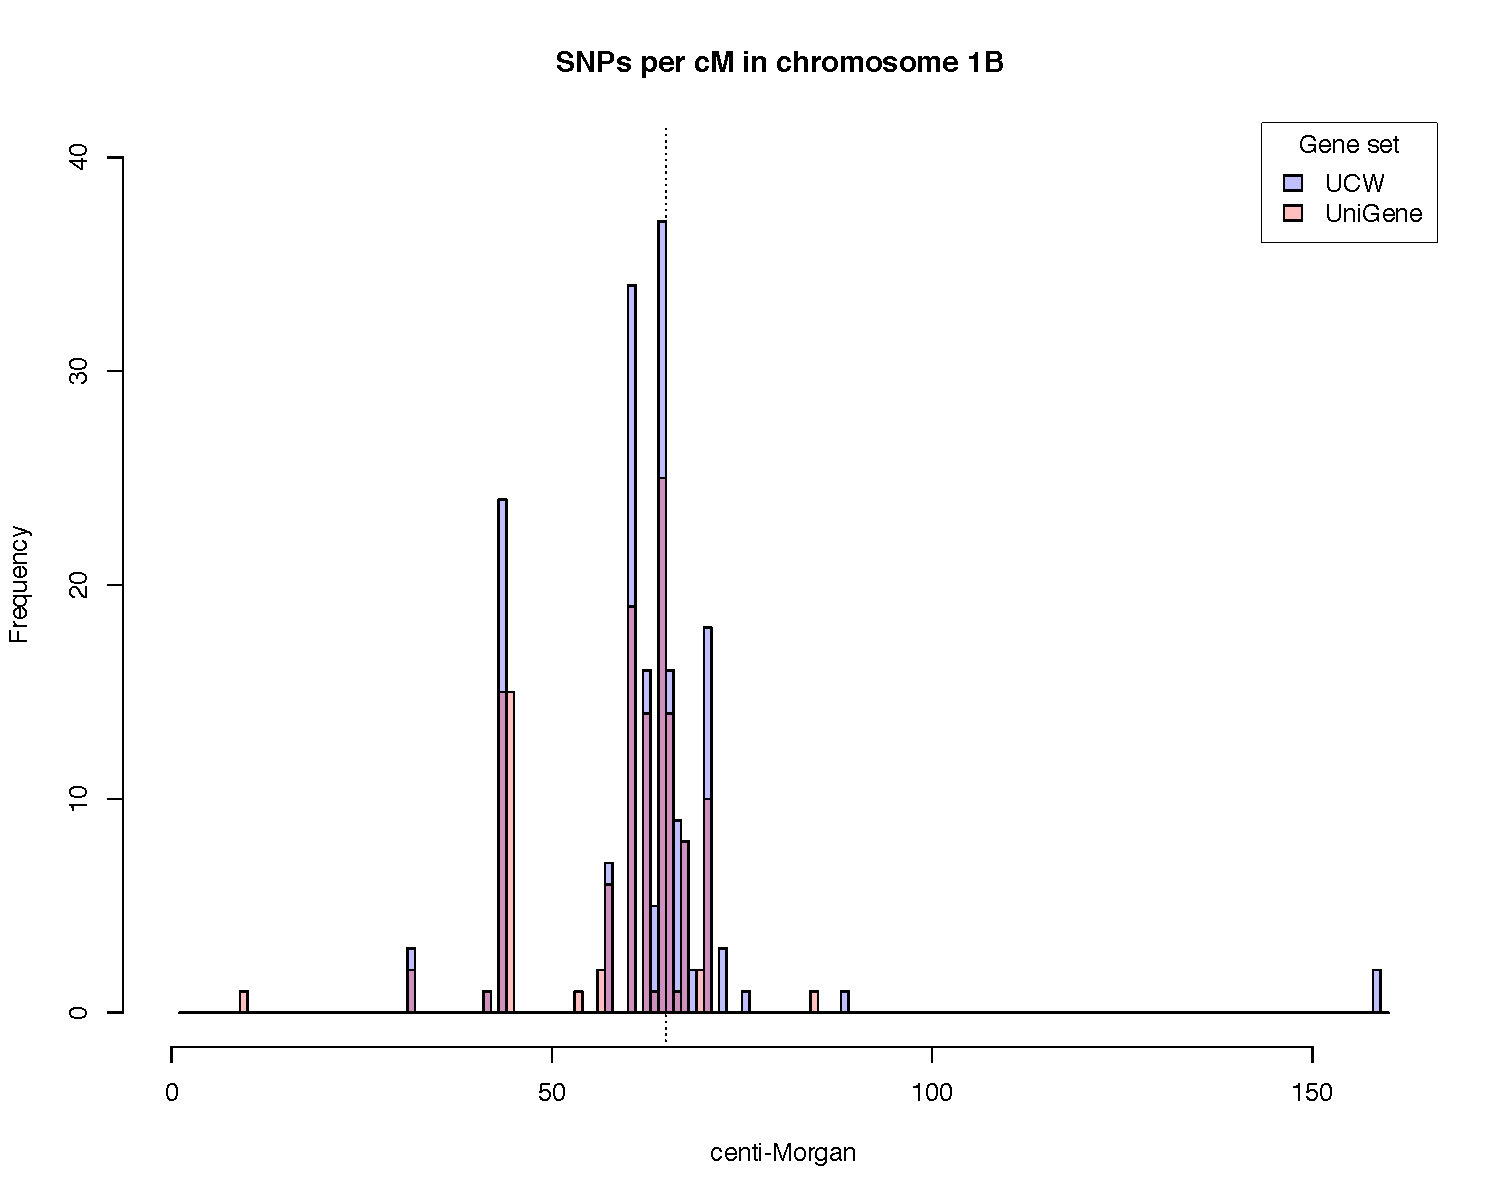
\includegraphics[width=1\textwidth]{Yr15/Figures/mapping/snpsBFR6crh1B.pdf}
  \end{subfigure}
  ~
  \begin{subfigure}{0.35\textwidth}
  \caption{}
   \label{fig:yr15:BFRValues1BS}
   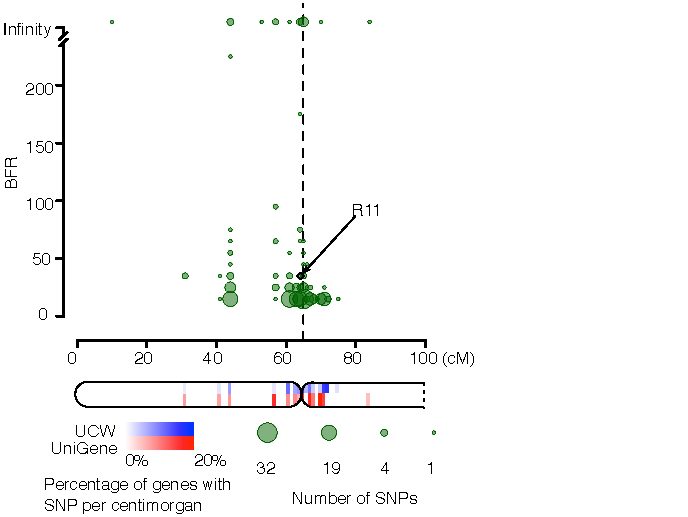
\includegraphics[width=1\textwidth]{Yr15/Figures/mapping/BFRValues1BS.pdf}
  \end{subfigure}
\caption[\textit{In silico} location of SNPs with BFR\textgreater6]{\textit{In silico} location of SNPs with $BFR>6$. (\subref{fig:yr15:snpsBFR6Chr1B}) Number of SNPs with $BFR>6$ per cM in chromosome 1B. (\subref{fig:yr15:BFRValues1BS}) BFRs of mapped genes with SNPs on chromosome 1B. The area of the circle represents the number of SNPs clustered by location (windows size: 10 cM) and BFR (window size: 5cM). R11 is the only marker near the \acrshort{yr15} locus that had a corresponding position in the genetic map. The percentage of genes with SNPs per cM is also illustrated based on UCW (blue) and UniGene (red) gene models. The centromere is imputed by the centre of a window of 10 cM where the short arm switches to the long in the genetic map. BFRs correspond to those from the mixed \textit{in silico} bulk S1 + S2 + S3/R1 + R2 + R3. Adapted from \citep{Ramirez-Gonzalez2015b}.} 
\label{fig:yr15:chr1}
\end{figure}

The \acrshort{css} assembly was used as a common reference between the reference genes and the 40,266 SNP markers published at the time \citep{Wang2014} to locate the SNPs with a $BFR>6$ (including $BFR=\infty$) in a genomic position (Figures \ref{fig:yr15:chr1}, \ref{fig:yr15:bfrs:0-6}).  
From the 1,582 SNPS across 1,173 genes,  only 678 SNPs ($43\%$, 474 genes) were successfully located in the genetic map. 
Since the \acrshort{css} assembly is quite fragmented, the low percentage of located SNPs can be because not all candidate SNPs had a corresponding scaffold that has at least one of the 40,266 markers in the genetic map. 
Even if the number of located SNPs was not enough to give a position for over $50\%$ of the SNPs from the parental line, the resolution of the genetic position SNPs that were assigned improved over just having the chromosome arm information from the CSS assembly. 
The mapping position further confirmed an enrichment of SNPs near the centromere of chromosome 1B with 325 out of 678 SNPs. 
Furthermore, 311 of those where located within an interval of 30cM (Figures \ref{fig:yr15:bfr6}, \ref{fig:yr15:snpsBFR6Chr1B}). 

Studies in diploid organisms using \acrshort{qtl}-Seq \citep{Takagi2013} or other \acrshort{ngs}-enabled genetic approaches \citep{James2013} have shown smooth curves with a defined peak in the region linked to the studied trait. 
In practice, we only observe clusters of SNPs with  enriched \acrshortpl{bfr} near the centromere of chromosome 1B (Figures \ref{fig:yr15:snpsBFR6Chr1B}, \ref{fig:yr15:bfr6}). 

\begin{figure}
	\centering
	\begin{subfigure}{0.4\textwidth}
	\caption{}
	\label{fig:yr15:bfr0}
	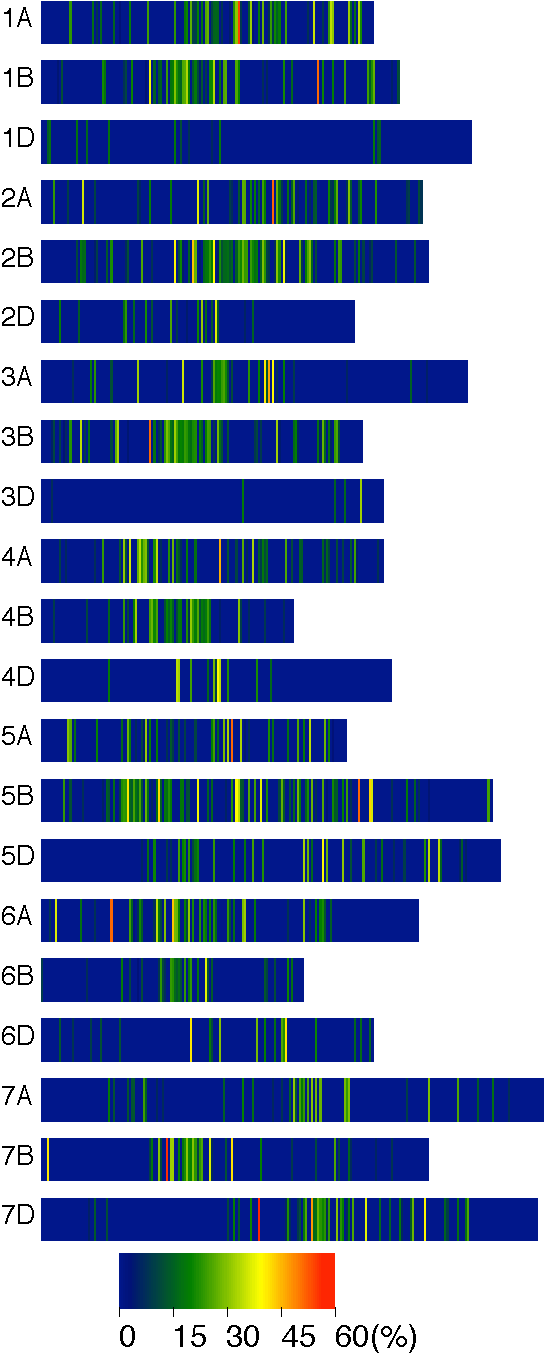
\includegraphics[height=0.55\textheight]{Yr15/Figures/mapping/snpsBFR0.pdf}
	\end{subfigure}
	~
	\begin{subfigure}{0.45\textwidth}
	\caption{}
	\label{fig:yr15:bfr6}
	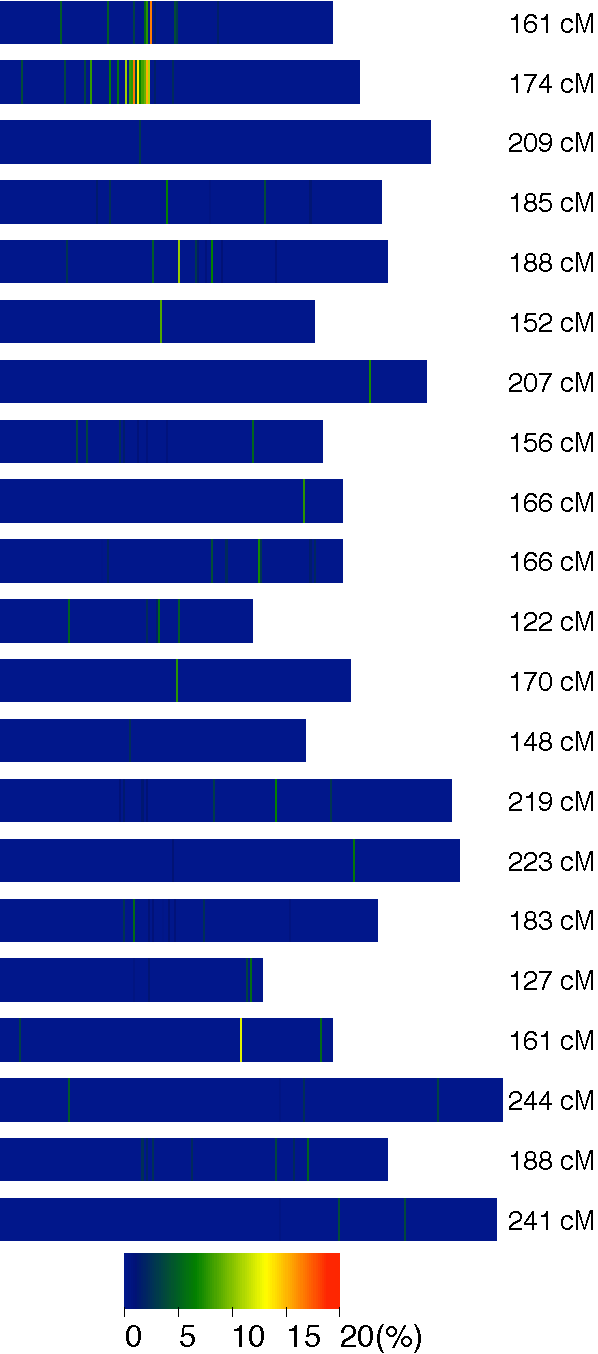
\includegraphics[height=0.55\textheight]{Yr15/Figures/mapping/snpsBFR6.pdf}
	\end{subfigure}
	\caption[Genetic location of genes with SNPs between AVS and Yr15.]{Genetic location of genes with SNPs between AVS and Yr15. The colour scale indicates the percentage of genes with SNPs per centi-Morgan (cM) across the 21 wheat chromosomes. The location of the genes was determined by the best alignment to the CSS scaffolds, and the location of these was determined by their position on a genetic map \citep{Wang2014} (\subref{fig:yr15:bfr0}). All the SNPs between progenitors. Note the lack of enrichment across any individual chromosome. (\subref{fig:yr15:bfr6}) SNPs with BFR$>$6. Note the enrichment in Chromosome 1B }
	\label{fig:yr15:bfrs:0-6}
\end{figure}

The location of the clusters with an enrichment of SNPs near the centromere is not expected on a random selection of genes, as the gene density increases with the distance to the centromere \citep{Akhunov2003}. 
This suggests that the experiment was successful on finding \acrshortpl{snp} linked to \acrshort{yr15}. 
There are several factor that prevent a clear peak; these include the biases induced by the differential expression and the fragmented reference sequence, with scaffolds that are not long enough to span genetic positions. 
Since there are several SNPs with a high BFR and the genetic map is not dense enough to locate a single region linked to \acrshort{yr15},  multiple criteria were needed to prioritise SNPs that were more likely to yield successful genetic markers.

\section{Assay selection} 
\label{yr15:assaySelection}
\begin{figure}
\centering
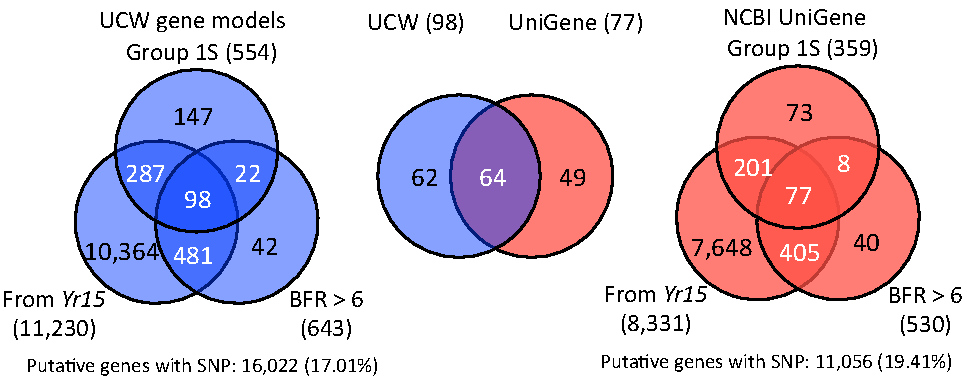
\includegraphics[width=1\textwidth]{Yr15/Figures/selection/snpSets.pdf}
\caption[Selection criteria for marker design]{Selection criteria for marker design. Venn diagrams based on the three selection criteria (SNP in the short arm of chromosome group 1; SNP has a $BFR>6$; and SNP is from the \acrshort{yr15} parent) for the UCW (blue) and UniGene (red) gene models. The centre diagram shows the intersection between common genes matching all three criteria across both data sets. Note that the numbers are not directly additive as in cases, multiple models from one reference set will relate to a single gene model in the other values. Published in \citep{Ramirez-Gonzalez2015b} }
\label{fig:yr15:snpset}
\end{figure}

Three independent criteria were used to prioritize the SNPs for marker development and validation: 

\begin{description}
\item[High BFR.] SNPs with a $BFR>6$ in at least two independent bulk replicates or in either of the \textit{in silico} mixes were selected to ensure consistency and recover SNPs with a low coverage on a particular bulk. 
\item[Group 1S.] SNPs that are in \acrshort{css} scaffolds in the short arm of chromosome group 1 were selected.
The selection included \glspl{snp} from the A, B and D genomes because the best hit to each gene model may be missing from the \gls{css} assembly.
Therefore, in cases where one or more of the homoeologous genes is missing from the reference, reads might be assigned to the wrong subgenome.
This is consistent with the \textit{in silico} genetic map and with previous studies \citep{Murphy2009,Peng2000,Grama1997}.
\item[\acrshort{yr15} parent.] The SNPs should originate from the \acrshort{yr15} parent to ensure that the SNP is coming from the \textit{T. diccocoides} introgression and not from a SNP in the \acrshort{avs} genetic background, who would be less useful in breeding programs with a different background.
\end{description}

Only SNPs meeting the three criteria were selected for further analysis. 

\begin{figure}
\centering
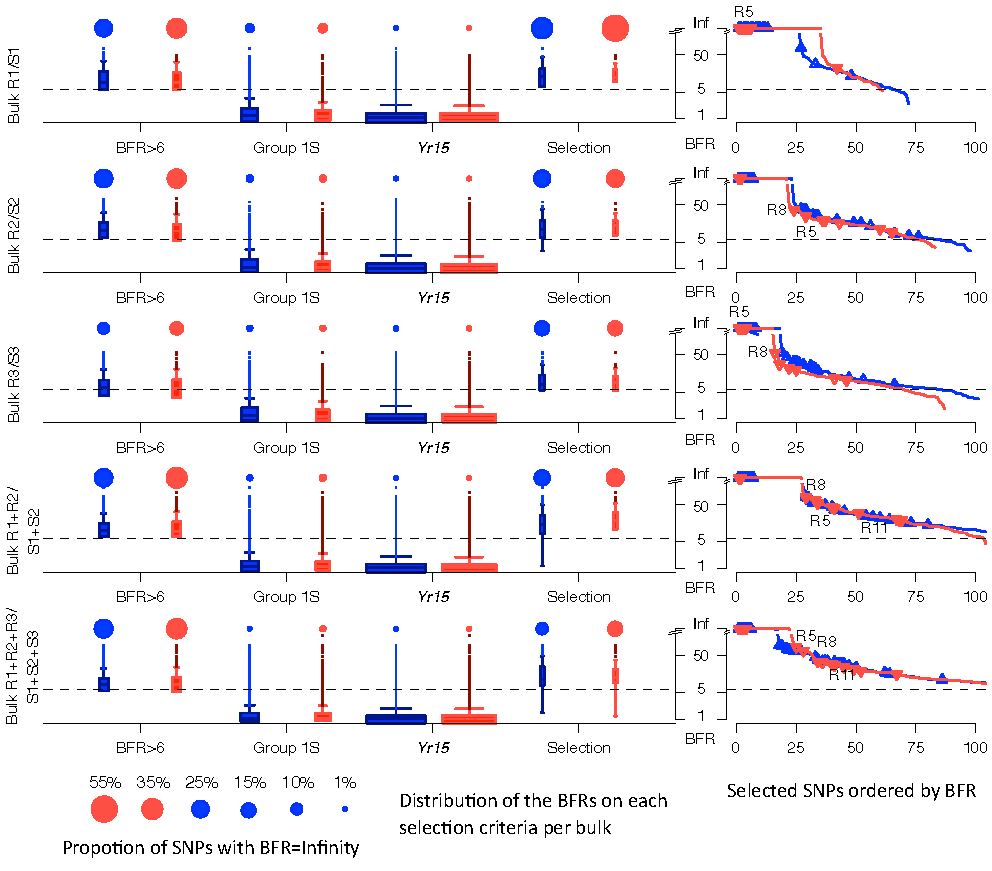
\includegraphics[width=1\textwidth]{Yr15/Figures/selection/selectionDetals.pdf}
\caption[BFRs of selected SNPs across bulks.]{BFRs of selected SNPs across the individual bulks and in silico mixes (UCW, red; UniGene, blue). The dotted line represents the BFR threshold of 6 (logarithmic scale). Left: Distribution of the BFRs for each selection criteria and the selected SNPs for validation. The circles on the top of each plot represent the percentage of SNPs with $BFR=\infty$. The Selection may include SNPs with $BFR<6$ when the same SNP has a higher score on the complementing reference (ie. $BFR>6$ on UCW, but $BFR<6$ on UniGenes). Right: The BFR values of selected SNPs were sorted in descending order across the different bulks and according to their origin. Validated SNPs are indicated by open triangles, and SNPs corresponding to markers R5, R8 and R11 are labelled across different bulks and mixes. Note that some SNPs are below the threshold in a specific bulk as they meet the BFR criteria across others. }
\label{fig:yr15:bfrDetailScore}
\end{figure}

Applying these multiple criteria, the number of genes with a putative SNP went down from over 27,000 to just 175; 77 and 98 from the UniGene and UCW gene sets, respectively.
As the two gene sets originate from independent sources, an overlap between the two selected sets is to be expected.
When we aligned the 77 and 98 genes from the two collections, we indeed found that around half of the genes overlap (Figure \ref{fig:yr15:snpset}). 
The 50 SNPs with the highest BFRs, out of the 175 genes, were selected for validation; fifteen of them were found to be redundant between references, resulting in a final set of 35 SNPs to validate. 

The separate bulks and the \textit{in silico} mixes were evaluated in detail to understand the behaviour and value of having multiple bulks. 
The initial expectation was that the number of SNPs with $BFR=\infty$ should drop in the mixes, as the improved coverage should reduce the number of instances where the absence of an allele is due to the lack of coverage on a particular sample. 
However, the opposite happened, the additional coverage in the \textit{in silico} mixes recovered SNPs in genes with a low expression at the time of the sampling (Figure \ref{fig:yr15:bfrDetailScore}).  
Some SNPs were present across all the samples, however the value of the BFR changed depending on the sample (e.g. marker R5). 
In some cases a \gls{snp} was missing in an individual bulk, but present in the rest and also in the mixes (e.g. marker R8). 
The main parameter affecting the scoring was the coverage in the sample for each particular gene, hence a strategy with a consistent coverage would be preferred for this kind of analysis.  
Previous studies have shown that a coverage of less than 5x is sufficient to call SNPs in model organisms with a high-quality reference \citep{Schneeberger2011}.
However, the results on this study are in line with other studies using populations for SNP calling \citep{Abe2012,Takagi2013}. 
The non-uniform distribution of the coverage in RNA-Seq experiments affects the number of reads that can be used to call for SNPs, especially on genes with a low expression level \citep{Mortazavi2008}. 

%!TEX root = ../../Main.tex
\begin{table}
\caption{ Number of genes (and SNPs) with a unique hit ($>99\%$ sequence identity) to a single wheat survey sequence scaffold. }
\label{tab:yr15:mappedGenes}
\centering
\begin{localsize}{9}{11}
\begin{tabular}{llrr@{\extracolsep{6pt}}rr@{\extracolsep{6pt}}rr}

\toprule
 \multicolumn{2}{l}{Chromosome 1}            &  \multicolumn{2}{c}{All SNPs} &  \multicolumn{2}{c}{BFR\ensuremath{>}6 }  &    \multicolumn{2}{c}{ \%  BFR\ensuremath{>}6 }       \\
  \cline{3-4}
  \cline{5-6}
  \cline{7-8}
                &            & SNP        & Genes  & SNP     & Genes  & SNPs               & Genes  \\
\midrule
 UCW            & Unique     & 5,283      & 1,245  & 311     & 214    & 5.89\%              & 17.19\% \\
                & Total      & 8,086      & 1,954  & 486     & 330    & 6.01\%              & 16.89\% \\
                & Percentage & 65.34\%     & 63.72\% & 63.99\%  & 64.85\% &                    &        \\
 \midrule
 UniGene        & Unique     & 3,687      & 745    & 213     & 139    & 5.78\%              & 18.66\% \\
                & Total      & 6,422      & 1,318  & 386     & 246    & 6.01\%              & 18.66\% \\
                & Percentage & 57.41\%     & 56.53\% & 49.17\%  & 56.07\% &                    &        \\
 \midrule
 UCW  & Unique     & 8,970      & 1,990  & 524     & 353    & 5.84\%              & 17.74\% \\
+              & Total      & 14,508     & 3,272  & 872     & 576    & 6.01\%              & 17.60\% \\
 UniGene       & Percentage & 61.83\%     & 60.82\% & 60.09\%  & 61.28\% &                    &        \\
\bottomrule
                &            &            &        &         &        &                    &        \\
\toprule
 All SNPs       &            &  \multicolumn{2}{c}{All SNPs} &  \multicolumn{2}{c}{BFR\ensuremath{>}6 }  &    \multicolumn{2}{c}{ \% BFR\ensuremath{>}6 }         \\
\cline{3-4}
\cline{5-6}
\cline{7-8}
                &            & SNP        & Genes  & SNP     & Genes  & SNPs               & Genes  \\
 \midrule
 UCW            & Unique     & 39,247     & 9,585  & 481     & 368    & 1.23\%              & 3.84\%  \\
                & Total      & 66,426     & 16,022 & 859     & 643    & 1.29\%              & 4.01\%  \\
                & Percentage & 59.08\%     & 59.82\% & 56.00\%  & 57.23\% &                    &        \\
 \midrule
 UniGene        & Unique     & 27,292     & 5,698  & 344     & 252    & 1.26\%              & 4.42\%  \\
                & Total      & 52,262     & 11,056 & 723     & 530    & 1.38\%              & 4.79\%  \\
                & Percentage & 52.22\%     & 51.54\% & 47.58\%  & 47.55\% &                    &        \\
 \midrule
 UCW  & Unique     & 66,539     & 15,283 & 825     & 620    & 1.24\%              & 4.06\%  \\
 +               & Total      & 118,688    & 27,078 & 1,582   & 1,173  & 1.33\%              & 4.33\%  \\
 UniGene       & Percentage & 56.06\%     & 56.44\% & 52.15\%  & 52.86\% &                    &        \\
\bottomrule
\end{tabular}
\end{localsize}
\end{table}


%TODO: maybe move to the discussion. 
Around $60\%$ of the gene models, across both references, had a unique hit with greater than 99\% sequence identity to a single \acrshort{css} scaffold (Table \ref{tab:yr15:mappedGenes}). 
\unsure{This sentence is not completely clear.}
This is likely because there is no unique homoeologue in the gene models, leading to reads, from two different homoeologues, mapping to the same region.
To reduce the number of spurious SNPs we used IUPAC ambiguity codes (Section \ref{lit:ambiguity}, \citet{Cornish-Bowden1985}) when two different alleles were observed.
This had the side effect that in order to keep only high confidence SNPs we required a higher coverage ($>20x$). 
On the original study introducing the BFR in tetraploid wheat, the authors show that increasing the coverage, from $8x$ to $16x$, reduces the putative SNPs by $60\%$, but the validated SNPs increase from $57\%$ to $83\%$ \citep{Trick2012}. 
Hence, a compromise between increasing the minimum coverage at the cost of reducing the SNP candidates had to be reached in line with the objectives and available resources for this particular study. 

\section {SNP Validation}

KASP assays were designed to validate and generate a genetic map of the \acrshort{yr15} locus for the 35 selected SNPs.
To automate the design of genome-specific primers for polyploid organisms PolyMarker was developed (Chapter \ref{cha:polymarker}).
Out of the 35 assays to design, 17 were designed as specific, 9 as semi-specific to chromosome 1BS, and 9 were not specific because there was no information for the homoeolouges on the \acrshort{css} scaffolds. 
PolyMarker also identified putative homoeologous variants (between genomes, as opposed to between varieties) that were in the list of candidate SNPs, but were not identified previously (Figure \ref{fig:poly:mask}; Table \ref{tab:yr15:polymarker}). 


\begin{figure}[b!]
\begin{subfigure}{0.31\textwidth}
\caption{}
\label{fig:yr15:r2}
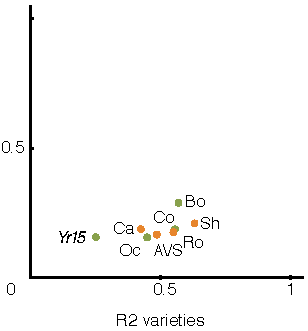
\includegraphics[width=1\textwidth]{Yr15/Figures/selection/R2.pdf}
\end{subfigure}
~
\begin{subfigure}{0.31\textwidth}
\caption{}
\label{fig:yr15:r8}
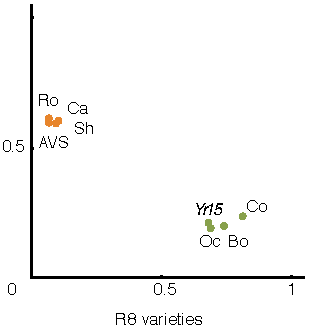
\includegraphics[width=1\textwidth]{Yr15/Figures/selection/R8.pdf}
\end{subfigure}
~
\begin{subfigure}{0.31\textwidth}
\caption{}
\label{fig:yr15:r8f2}
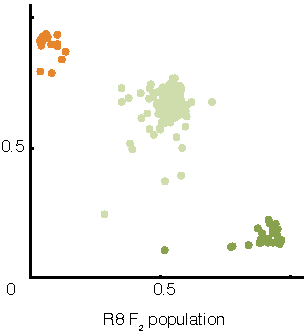
\includegraphics[width=1\textwidth]{Yr15/Figures/selection/R8F2.pdf}
\end{subfigure}

\caption[KASP output from the wheat variety panel]{KASP output from the wheat variety panel with (Ochre, Boston, Cortez) and without (Robigus, Cadenza and Shamrock) \acrshort{yr15}. Marker  R2 (\subref{fig:yr15:r2}) is monomorphic while R8 (\subref{fig:yr15:r8})  is polymorphic between varieties known to carry the gene.  Marker R8 results for the F2 population (\subref{fig:yr15:r8f2}) showing three distinct clusters. The central cluster (light green) is comprised of heterozygous individuals, whereas clusters near the axes are homozygous for either AVS (VIC; orange) or \acrshort{yr15} (FAM; dark green).}
\end{figure}


To validate if the 35 SNPs were polymorphic across the parents and diagnostic for \acrshort{yr15} we tested them in the progenitors plus six commercial varieties, three containing \acrshort{yr15} (Ochre, Boston and, Cortez) and three without it (Shamrock, Robigus and, Cadenza).
Two of the lines without \acrshort{yr15} have \textit{T. diccocoides} in their pedigree (Shamrock and Robigus), as it is the donor species of \textit{Yr15} \citep{mcintosh1995}. 
This test panel allows to test if the SNPs are only diagnostic to \textit{T. diccocoides} instead of \acrshort{yr15}.
On the test panel, 28 ($80\%$) SNPs were polymorphic across the parents and three of them where diagnostic to \textit{Yr15} (R5, R8, R33).
From the five homoeologous SNPs, three of them were monomorphic and two polymorphic, suggesting that PolyMarker is effective on detecting which assays are less likely to work (Table \ref{tab:yr15:markersToTest}; Figure \ref{fig:yr15:r2},\subref{fig:yr15:r8}).
The segregation of the SNPs in the full $F_{2}$ population (Section \ref{sub:mappingPopulation}, Figure \ref{fig:yr15:r8f2}) and a genetic map was produced (Section \ref{yr15:geneticMap}).   



%!TEX root = ../../Main.tex
\begin{sidewaystable}
\caption{Primer details for the markers to validate. }
\centering
\label{tab:yr15:polymarker}
\begin{localsize}{6}{9}

\begin{tabular}{lllllll}
\toprule
 Assay ID   & Polymorphism\_type   & AVS-specific primer         & Yr15-specific primer        & Common primer               & Specificity             & Orientation   \\
\midrule
 R1         & non-homeologous     & aactggtaatggtgcagCgG        & aactggtaatggtgcagCgC        & ttcaggataacacAggagatgtT     & chromosome\_semispecific & reverse       \\
 R2         & non-homeologous     & acatcaattcttcaggaaagctctaC  & acatcaattcttcaggaaagctctaT  & gcacagcttctcgtgttcTT        & chromosome\_specific     & forward       \\
 R3         & non-homeologous     & acgtggagaacctagattgcG       & acgtggagaacctagattgcC       & ccttttaggtgcgccaactT        & chromosome\_semispecific & reverse       \\
 R4         & non-homeologous     & agactctttgggcagtggatC       & agactctttgggcagtggatT       & cctcgggcgatctattctcT        & chromosome\_specific     & forward       \\
 R5         & non-homeologous     & agtcaacttggattacactgaagtT   & agtcaacttggattacactgaagtC   & agatatcacactgaacatactgatgaG & chromosome\_specific     & reverse       \\
 R6         & non-homeologous     & caagatgaagatgaagaggaatatgaT & caagatgaagatgaagaggaatatgaC & gCttgaccctgtaatcatactcG     & chromosome\_semispecific & forward       \\
 R7         & non-homeologous     & caccaccaTggaggccaC          & caccaccaTggaggccaT          & cgccgtggtagtgtccgG          & chromosome\_specific     & forward       \\
 R8         & non-homeologous     & cagatccccggttctctcaaG       & cagatccccggttctctcaaA       & cccccaaatgatcgagaata        & chromosome\_inspecific   & reverse       \\
 R9         & non-homeologous     & caggtgctgaaatgcatcC         & caggtgctgaaatgcatcT         & cggcctatcttcaggtctgt        & chromosome\_inspecific   & reverse       \\
 R10        & non-homeologous     & cattcgtcgcgccttctacG        & cattcgtcgcgccttctacA        & tcctaactcatatgcatgactcAC    & chromosome\_specific     & reverse       \\
 R11        & non-homeologous     & ccattctgatcaaggtcactgtcG    & ccattctgatcaaggtcactgtcA    & ttctgtaTggcaaCgggagC        & chromosome\_specific     & reverse       \\
 R12        & homeologous         & cttagccagtgaaccAggcC        & cttagccagtgaaccAggcT        & ggctgtttgttacCgtggaG        & chromosome\_specific     & reverse       \\
 R14        & non-homeologous     & gacTacAggtgcgatcccC         & gacTacAggtgcgatcccT         & ctcgcctgccagtcgTaT          & chromosome\_specific     & forward       \\
 R15        & homeologous         & gactagggctaccAttgttgA       & gactagggctaccAttgttgC       & agccctgCtaacaatggcaA        & chromosome\_specific     & reverse       \\
 R16        & non-homeologous     & gatgtaagcTAtgactggCgC       & gatgtaagcTAtgactggCgT       & tgcaactgatctttagcaggC       & chromosome\_semispecific & reverse       \\
 R17        & non-homeologous     & gcaAcaacaaCaaCaagtggT       & gcaAcaacaaCaaCaagtggC       & cctcaacctgcttgttgttgT       & chromosome\_specific     & forward       \\
 R19        & non-homeologous     & gcctgatttttaattcgctccaG     & gcctgatttttaattcgctccaA     & agagcactgatgatgacccC        & chromosome\_specific     & reverse       \\
 R20        & non-homeologous     & gctgtatcctcttgaaaaaggcT     & gctgtatcctcttgaaaaaggcC     & ttaggcatgtcagaaatgtagaaaa   & chromosome\_semispecific & forward       \\
 R21        & non-homeologous     & gcttcaaacatgccggctG         & gcttcaaacatgccggctT         & cggtctttttcaaccagggC        & chromosome\_semispecific & forward       \\
 R22        & homeologous         & gctTgtCttaaagccAtttccA      & gctTgtCttaaagccAtttccG      & gcctatcgttCgctaaactctaacT   & chromosome\_specific     & reverse       \\
 R23        & non-homeologous     & gctttaggcactatggattcAcC     & gctttaggcactatggattcAcT     & caggtttctgttcgacctcA        & chromosome\_specific     & forward       \\
 R24        & non-homeologous     & ggaggtcctacacgcgtctT        & ggaggtcctacacgcgtctG        & ctccaaaagaggggcatcattT      & chromosome\_semispecific & forward       \\
 R25        & non-homeologous     & gggttcctcacctgcgcC          & gggttcctcacctgcgcT          & ctctTtgcaatcggccagc         & chromosome\_inspecific   & reverse       \\
 R26        & non-homeologous     & gtCttcgcCggcacCacC          & gtCttcgcCggcacCacT          & agtggatcttgccgatctcg        & chromosome\_inspecific   & forward       \\
 R28        & non-homeologous     & tagatgagaccttggaCggA        & tagatgagaccttggaCggG        & cagtcatctaatgcggaacattcA    & chromosome\_semispecific & reverse       \\
 R29        & non-homeologous     & TatggtGtggccTtccccG         & TatggtGtggccTtccccA         & cgagctcgctgatgaacttG        & chromosome\_specific     & forward       \\
 R30        & non-homeologous     & tcagcagcccttttaacccaA       & tcagcagcccttttaacccaT       & agtaaatcgggcacggttgt        & chromosome\_inspecific   & reverse       \\
 R31        & homeologous         & tcatccatgtatatGaaTccaagcC   & tcatccatgtatatGaaTccaagcA   & tcacgcctgcaacAttcaaaT       & chromosome\_specific     & reverse       \\
 R32        & homeologous         & tccaatcttatggctttgcttctG    & tccaatcttatggctttgcttctT    & caggtgatgtagatgctgagaC      & chromosome\_semispecific & reverse       \\
 R33        & non-homeologous     & tccttcctgctatagctgaaagG     & tccttcctgctatagctgaaagT     & ccctttgcctgccatgtaga        & chromosome\_inspecific   & forward       \\
 R34        & non-homeologous     & tctgagatgatgatactTtgtggG    & tctgagatgatgatactTtgtggA    & actggggatgccctctgtat        & chromosome\_inspecific   & forward       \\
 R35        & non-homeologous     & tgaaagagtggaatttcttgttgT    & tgaaagagtggaatttcttgttgC    & ctttTagctgcttaattctattgcttC & chromosome\_specific     & forward       \\
 R36        & non-homeologous     & tgaaatgccttgtcaatgccA       & tgaaatgccttgtcaatgccG       & ATGCGAATTGGGGAATTAAA        & chromosome\_inspecific   & reverse       \\
 R37        & non-homeologous     & tgcatatgcctgaagagactcG      & tgcatatgcctgaagagactcA      & tgtccacctactcaagtctgc       & chromosome\_inspecific   & reverse       \\
 R38        & non-homeologous     & tgGcCaagTtTttctgcaagaT      & tgGcCaagTtTttctgcaagaG      & tgtaggaaggaactcCgaagtA      & chromosome\_specific     & forward       \\
 R40        & non-homeologous     & tgcatatgcctgaagagactcA      & tgcatatgcctgaagagactcG      & agtccgctaaagcattgcct        & chromosome\_nonspecific  & reverse       \\
 R43        & non-homeologous     & tcgctgatttcatcatgtcccA      & tcgctgatttcatcatgtcccG      & tcaggtgctgcaaatttgagG       & chromosome\_semispecific & forward       \\
\bottomrule
\end{tabular}
\end{localsize}
\end{sidewaystable}

%!TEX root = ../../Main.tex
\begin{sidewaystable}
\caption{Results of validation of primers on the progenitors (\acrshort{avs} and \acrshort{yr15}, varieties known to contain \acrshort{yr15} (Cortez, Ochre and, Boston) } and, varieties without \acrshort{yr15} (Robigus, Cadenza and, Shamrock). Shamrock and Robigus have \textit{T. dicoccoides} introgressions. The underlined markers are the diagnostic triplet. 

\label{tab:yr15:markersToTest}
\begin{localsize}{6}{9}
\centering
\begin{tabular}{llllllll|lllllll}
\toprule
Assay &             &                    &        & \begin{sideways}Yr15\end{sideways}    & \begin{sideways}Ochre\end{sideways}  & \begin{sideways}Boston\end{sideways}    & \begin{sideways}Cortez\end{sideways}    & \begin{sideways}Shamrock \end{sideways}    & \begin{sideways}Robigus\end{sideways}    & \begin{sideways}Cadenza\end{sideways}    & \begin{sideways}AVS\end{sideways} & \begin{sideways}Polymorphic\end{sideways} & \begin{sideways}Linked \acrshort{yr15}\end{sideways}  &\\
%\cline{5-8}
%\cline{9-12}
 ID   & Gene set    & Gene model name    & SNP    & \multicolumn{4}{c}{\acrshort{yr15}+ } & \multicolumn{4}{c}{\acrshort{yr15}- } &   &      & comment                 \\
\midrule
 R1         & UCW         & UCW\_Tt-k55\_contig\_8830;tt-k21\_contig\_10204                      & C341G  & A      & H         & A        & A        & A            & -         & A         & B     & Yes           & * &   segregation distortion                      \\
 R2         & UniGene v60 & gnl|UG|Ta\#S13126619                                             & C491T  & B      & B         & B        & B        & B            & B         & B         & B     & No            & -                      &                         \\
 R3         & UCW         & contig95240                                                     & C220G  & H      & B         & B        & B        & B            & B         & B         & B     & Yes           & Yes                    &                         \\
 R4         & UCW         & contig105384                                                    & C1227T & A      & B         & B        & B        & B            & B         & B         & B     & Yes           & Yes                    &                         \\
 R5         & UniGene v60 & gnl|UG|Ta\#S58861868                                             & A214G  & A      & A         & A        & A        & B            & B         & B         & B     & Yes           & Yes                    &                         \\
 \midrule
 R6         & UCW         & KukriC706\_1                                                     & T2979C & A      & H         & B        & B        & B            & B         & H         & H     & Yes           & No                     &                         \\
 R7         & UniGene v60 & gnl|UG|Ta\#S37932863                                             & C281T  & H      & A         & A        & A        & B            & B         & A         & B     & Yes           & No                     &                         \\
 R8         & UniGene v60 & gnl|UG|Ta\#S58863387                                             & T241C  & B      & B         & B        & B        & A            & A         & A         & A     & Yes           & Yes                    &                         \\
 \midrule
 R9         & UniGene v60 & gnl|UG|Ta\#S58892239                                             & C303T  & H      & B         & A        & B        & B            & B         & H         & B     & Yes           & No                     &                         \\
 R10        & UCW         & UCW\_Tt-k63\_contig\_79829                                         & C207T  & H      & A         & B        & A        & B            & B         & B         & B     & Yes           & Yes                    &                         \\

 R11        & UCW         & UCW\_Tt-k45\_contig\_39011                                         & C726T  & A      & A         & A        & H        & -            & B         & B         & B     & Yes           & Yes                    &                         \\
  \midrule
  R12        & UCW         & contig50308                                                     & G587A  & -      & H         & H        & H        & B            & B         & A         & B     & Yes           & Yes                    &                         \\
 R14        & UniGene v60 & gnl|UG|Ta\#S44692929                                             & C549T  & A      & A         & -        & A        & A            & B         & -         & B     & Yes           & Yes                    &                         \\
 R15        & UCW         & UCW\_Tt-k51\_contig\_2344;tt-k55\_contig\_2091                       & T686G  & A      & A         & A        & A        & A            & A         & A         & A     & No            & -                      &                         \\
 R16        & UniGene v60 & gnl|UG|Ta\#S17898149                                             & G227A  & A      & A         & B        & A        & B            & B         & B         & B     & Yes           & Yes                    &                         \\
 R17        & UCW         & CL3339Contig1                                                   & T509C  & H      & H         & H        & H        & H            & H         & H         & H     & No            & -                      &                         \\
 R19        & UCW         & UCW\_Tt-k21\_contig\_8407;tt-k61\_contig\_5972                       & C1405T & A      & B         & B        & B        & B            & B         & B         & B     & Yes           & Yes                    &                         \\
 R20        & UCW         & UCW\_Tt-k21\_contig\_8407;tt-k61\_contig\_5972                       & T1102C & A      & B         & B        & B        & -            & B         & B         & B     & Yes           & Yes                    &                         \\
 R21        & UCW         & UCW\_Tt-k31\_contig\_53804;tt-k41\_contig\_31582                     & G1810T & H      & B         & B        & B        & B            & B         & B         & B     & Yes           & Yes                    &                         \\
 R22        & UCW         & UCW\_Tt-k31\_contig\_14966                                         & T408C  & A      & A         & A        & A        & A            & A         & A         & B     & Yes           & Yes                    &                         \\
 R23        & UCW         & UCW\_Tt-k51\_contig\_12731;tt-k55\_contig\_13077;tt-k61\_contig\_18734 & C50T   & A      & H         & H        & H        & H            & -         & H         & B     & Yes           & Yes                    &                         \\
 R24        & UCW         & UCW\_Tt-k55\_contig\_8830;tt-k21\_contig\_10204                      & T3005G & H      & H         & B        & H        & B            & B         & B         & B     & Yes           & Yes                    &                         \\
 R25        & UCW         & UCW\_Tt-k63\_contig\_79829                                         & G184A  & A      & A         & A        & A        & H            & H         & A         & A     & No            & -                      &                         \\
 R26        & UCW         & UCW\_Tt-k21\_contig\_3794                                          & C702T  & H      & A         & B        & A        & B            & B         & B         & B     & Yes           & Yes                    &                         \\
 R28        & UCW         & KukriC3701\_1                                                    & T1053C & A      & A         & B        & A        & B            & B         & B         & B     & Yes           & Yes                    &                         \\
 R29        & UCW         & UCW\_Tt-k55\_contig\_8640;tt-k41\_contig\_8875                       & G783A  & H      & A         & B        & A        & B            & B         & B         & B     & Yes           & Yes                    &                         \\
 R30        & UCW         & UCW\_Tt-k55\_contig\_8830;tt-k21\_contig\_10204                      & T2184A & A      & A         & B        & A        & B            & B         & A         & B     & Yes           & Yes                    &                         \\
 R31        & UCW         & UCW\_Tt-k45\_contig\_22098                                         & G683T  & A      & B         & A        & B        & B            & B         & A         & B     & Yes           & Yes                    &                         \\
 R32        & UCW         & UCW\_Tt-k21\_contig\_33188;tt-k25\_contig\_30647                     & C596A  & H      & A         & A        & A        & A            & A         & A         & H     & No            & -                      &                         \\
 R33        & UniGene v60 & gnl|UG|Ta\#S58861868                                             & G486T  & A      & A         & A        & A        & B            & B         & B         & B     & Yes           & Yes                    &                         \\
 R34        & UCW         & UCW\_Tt-k31\_contig\_34099                                         & G1713A & H      & A         & B        & -        & B            & B         & B         & B     & Yes           & No                     &                         \\
 R35        & UniGene v60 & gnl|UG|Ta\#S58900202                                             & T889C  & A      & B         & B        & B        & B            & B         & B         & B     & Yes           & Yes                    &                         \\
 R36        & UCW         & UCW\_Tt-k55\_contig\_8830;tt-k21\_contig\_10204                      & T2349C & H      & H         & H        & H        & H            & -         & H         & B     & Yes           & Yes                    &                         \\
 R37        & UCW         & UCW\_Tt-k31\_contig\_34099                                         & C846T  & B      & B         & B        & B        & B            & B         & B         & B     & No            & -                      &                         \\
 R38        & UniGene v60 & gnl|UG|Ta\#S58840501                                             & T179G  & B      & B         & B        & B        & B            & B         & B         & B     & No            & -                      &                         \\
 R40        & UCW         & UCW\_Tt-k31\_contig\_34099                                         & C846T  & A      & H         & B        & A        & -            & B         & B         & B     & Yes           & No                     & based on barley synteny \\
 R43        & UniGene v60 & gnl|UG|Ta\#S58843705                                             & G268A  & A      & B         & B        & -        & -            & B         & -         & B     & Yes           & Yes                    & based on barley synteny \\
\bottomrule
\end{tabular}
\end{localsize}
\end{sidewaystable}


\section{Genetic map} 
\label{yr15:geneticMap}


Initially, the 28 polymorphic markers were used to genotype a subset of 66 plants from the $F_{2}$ population. 
From those, 23 (82\%) were linked to \acrshort{yr15} and several markers map in a small interval around \acrshort{yr15} (Figure \ref{fig:yr15:initialMap}; Table \ref{tab:yr15:markersToTest}), confirming that the multiple-criteria strategy(Section \ref{yr15:assaySelection}) for selecting candidate SNPs was effective. 
Then, the complete $F_{2}$ population was assessed with:
\begin{itemize}	
	\item  the seven markers that were most closely linked to \acrshort{yr15}, including two of the diagnostic markers from the variety panel (R5 and R8),
	\item The flanking \acrshort{ssr} microsatellite markers used by UK breeders for germoplasm selection (\textit{Xbarc8} and \textit{Xgwm413}).  These correspond to the best markers available to breeders at the time of the study.
	\item A marker based on barley-wheat synteny (R43) which met the selection criteria, but was not on the original set of 50 markers with high BFR. 
\end{itemize}

The $F_{2}$ population consisted on 232 plants with phenotypic information, of those 196 where genotyped reliably (no more than one data point missing). 
Using the eight SNP markers and 2 SRRs, the \acrshort{yr15} locus was mapped to an interval of 0.77cM, with R8/xgwm413 0.26cM distal, and R5/R11 0.77cM proximal from \acrshort{yr15} (Figure \ref{fig:yr15:finalMap},\subref{fig:yr15:mapDetails}). 


\begin{figure}
	\centering
	\begin{subfigure}{0.45\textwidth}
	\caption{}
	\label{fig:yr15:initialMap}
	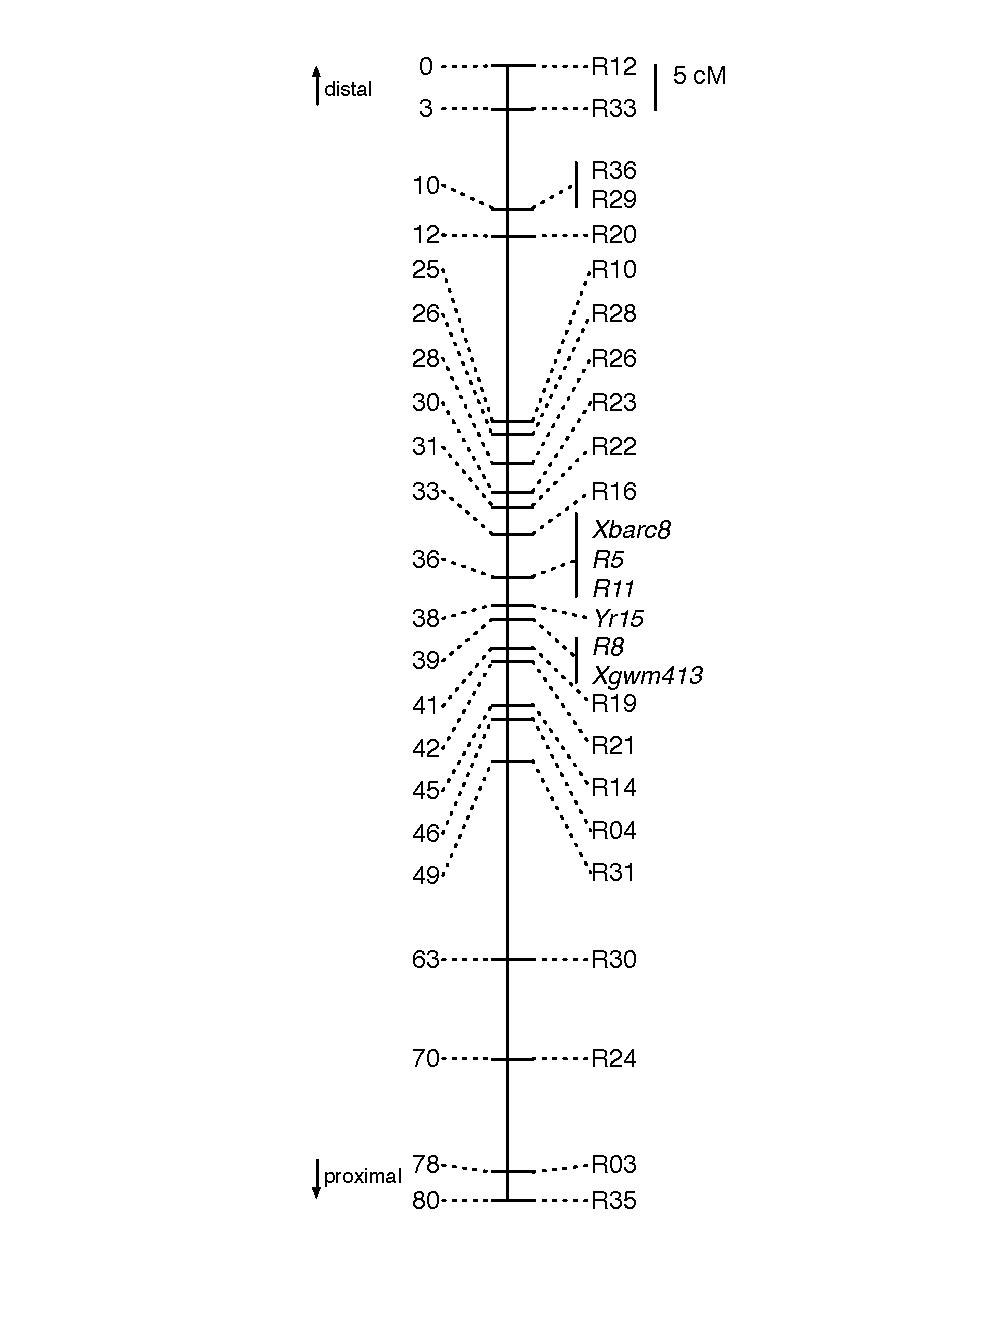
\includegraphics[height=0.45\textheight]{Yr15/Figures/selection/initialMap.pdf}
	\end{subfigure}
	~
	\begin{subfigure}{0.45\textwidth}
	\caption{}
	\label{fig:yr15:finalMap}
	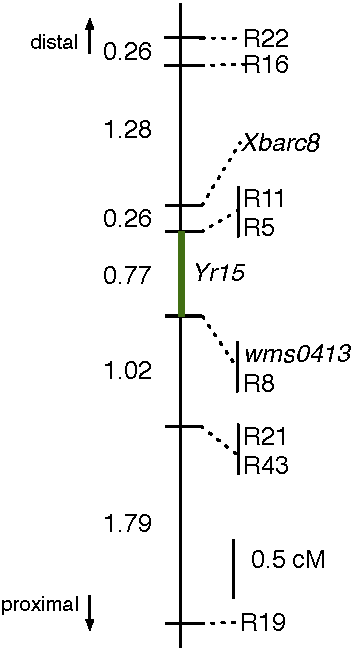
\includegraphics[height=0.45\textheight]{Yr15/Figures/selection/fineMap.pdf}
	\end{subfigure}

	\begin{subfigure}{1\textwidth}
	\caption{}
	\label{fig:yr15:mapDetails}
	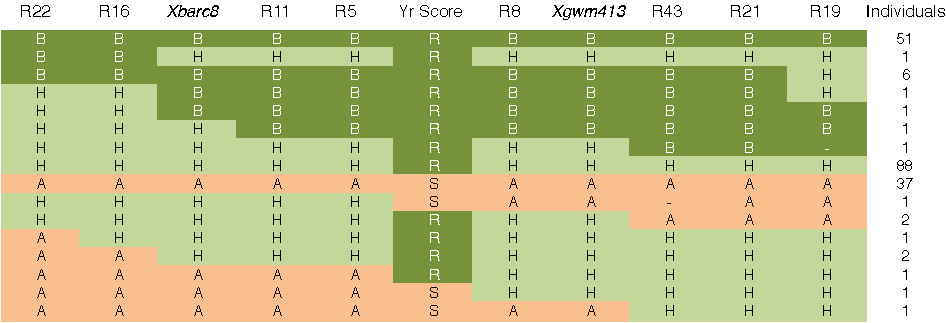
\includegraphics[width=1\textwidth]{Yr15/Figures/selection/mapDetails.pdf}
	\end{subfigure}
	

	\caption[Genetic maps for \acrshort{yr15}.]{Genetic maps for \acrshort{yr15}. (\subref{fig:yr15:initialMap}) Genetic map of the test panel from 50 individuals. (\subref{fig:yr15:finalMap}) Genetic map from 196 individuals from the full population only with the 8 markers previously identified as closer to the \acrshort{yr15} locus. (\subref{fig:yr15:mapDetails})Graphical genotype of the 196 $F_{2}$ individuals used to develop the genetic map. The alleles are abbreviated according to their origin: A: AVS; B: \textit{Yr15} and H: Heterozygous. Missing calls are indicated by a hyphen.}
\end{figure}

The sub-cM resolution is expected in a $F_{2}$ population of 196 individuals, as 392 gametes should provide n average resolution of 0.26{}cM. 
\unsure{I assume here that mas pipelines prefer now to use SNPs.}
Despite the fact that none of the selected markers have perfect linkage to \acrshort{yr15}, the resulting genetic map is an improvement in the resolution of the map for the locus and it enables the shift to SNP markers from microsatellites. The former has become the preferred marker system in \acrshort{mas} pipelines in breeding programmes. 


\section{Methods}
\label{yr15:methods}

\begin{figure}
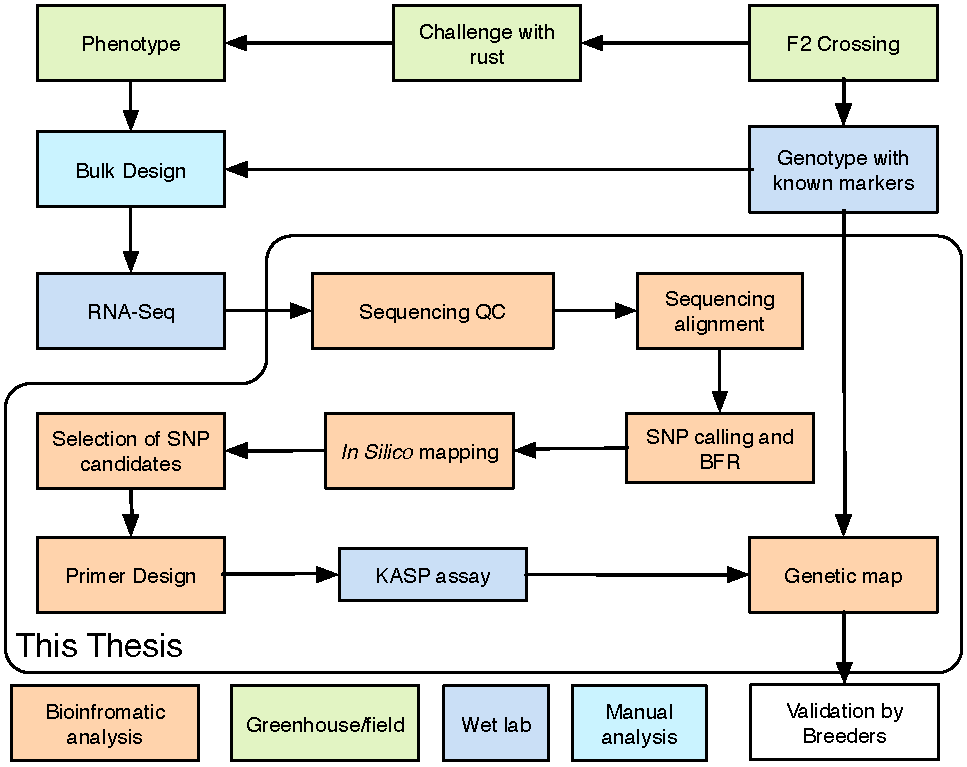
\includegraphics[width=1\textwidth]{Yr15/Figures/pipeline.pdf}
\caption{Steps used to go from the $F_{2}$ population to the genetic map.}
\end{figure}

The data analysis for this PhD required the use of some standard tools and custom developed code. 
All the code produced for this project is available and updated on the a github repository: \url{https://github.com/TGAC/bioruby-polyploid-tools}. 
For clarity, the snippets of code on this section had been simplified by removing the exception handling, type checks and caching mechanism.

\subsection{Base-call and Quality Control of sequencing reads}
The raw output from the Illumina HiSeq 2000 was processed with Casava v1.8 \citep{casavaBCL}. 
Lanes 1 and 2, containing multiplexed bulks (Table \ref{tab:yr15:reads}) was demultiplexed with a tolerance of 1 mismatch in the barcode. 
Lanes 3 and 4 contained the parental sequences without a barcode. 
The FastQ files where left compressed and in chunks of 40,000, as the default for the BCL conversion pipeline from Casava to allow parallel processing in a cluster environment. 
The quality of the sequencing lanes was assessed with FastQC v0.10.1 \citep{fastqc}. 

\subsection{Alignment reads to gene models}
The RNA-Seq reads were aligned with BWA 0.5.9 \citep{Li2009} to the wheat UniGene database v60 \citep{PontiusJUWagnerL2002} and to the UCW gene models \citep{Krasileva2013}, including the \textit{T. turgidum} and complementary ORFs \citep{MASWheat2013}.
The alignments where sorted and stored as single BAM files to have random access \citep{Li2009a}. 
%\unsure{ Snippet with submission of the alignments. However I have not got access to the old cluster files.}


\subsection{Bulk Frequency Ratios and SNP calling}
\label{yr15:sub:bfr}
To avoid the creation of several temporary files with the coverage information on all the bases I developed a \texttt{Ruby} pipeline based on the \texttt{bio-samtools} library \citep{Ramirez-Gonzalez2012}, and some of the improvements to work with pileups were published as a follow-up on the library \citep{Etherington2015}.
To call for the consensus, the function \texttt{Bio::DB::Sam::mpileup} is called to generate the pileup of each gene. 
As the pileups are used several times during the analysis, a function that caches the current pileup is implemented.
The consensus is called by counting how many times each base appears, and if the number of bases is higher than \texttt{minumum\_ratio\_for\_iuap\_consensus} the base is added to the set of possible bases \citep{Cornish-Bowden1985} 
If there is no coverage at a certain position, the reference base is used, and set as lowercase. 
If the set of called bases is not empty, the ambiguity code for the observed bases is called, and set as upper case (Listing \ref{lst:yr15:consensus}).
The minimum ratio was done on 0.2 (20\%), as it allows calling for a consensus even when more than one homoeologue is mapping to the same reference.

\begin{code}[language=Ruby,caption=Method to call for the consensus on progenitors from a pileup, label=lst:yr15:consensus]
def consensus_iuap(minumum_ratio_for_iuap_consensus)
  minumum_ratio_for_iup_consensus
  @consensus_iuap = self.ref_base.downcase
  bases = self.bases
  tmp = String.new
  bases.each do |k,v|
    if v/self.coverage > minumum_ratio_for_iup_consensus
      tmp << k[0].to_s
    end 
    if tmp.length > 0
      @consensus_iuap = Bio::NucleicAcid.to_IUAPC(tmp)
    end
  end 
  @consensus_iuap.upcase
end
\end{code}

Then, to calculate the \acrshortpl{bfr} as shown on Figure \ref{fig:yr15:bfr} extra extensions for the \texttt{Bio::DB::Pileup} were added to get the actual number of bases in the pile (to exclude short insertions and deletions; Listing \ref{lst:yr15:cov}), and to calculate the SNP-Index (Listing \ref{lst:yr15:ratio}).  

\begin{code}[language=Ruby,caption=\texttt{base\_coverage} gets the number of bases called from a single pileup., label=lst:yr15:cov]
def base_coverage
  total = 0
  @bases.each do |k,v|
    total += v  
  end
  total
end
\end{code}

\begin{code}[language=Ruby,caption=\texttt{base\_ratios} gets the SNP-Index on a single pileup., label=lst:yr15:ratio]
def base_ratios
  return @base_ratios if @base_ratios
  bases = self.bases
  @base_ratios = Hash.new
  bases.each do |k,v| 
    @base_ratios[k] = v.to_f/self.base_coverage.to_f 
  end
  @base_ratios
 end
\end{code}

To calculate \acrshortpl{bfr} the class \texttt{Bio::BFRTools::Container} was implemented to contain all the \texttt{BIO:DB:Sam} objects corresponding to the progenitors and the bulks. 
The class \texttt{Bio::BFRTools::BFRRegion}  was implemented to contain the ratios and consensus sequences of each region. 
The method \texttt{bfr} uses the calculated SNP-Indices on every position, from the point of view of both progenitors (lines 15-16: Listing \ref{lst:yr15:bfr}, and in the case of lack of coverage the value is set to 0 or \texttt{Infinity} (lines 8-13), depending on the progenitor where the base is not called at all. 
Using this design where the values of each region are calculated at once reduces the number of times the pileup needs to be generated for each sample and allows to have in a single place in memory all the elements to calculate the \acrshortpl{bfr}, without having to write any temporary files on disc. 
Also, the fact that the calculation of each region is independent from that for other regions, it is possible to use a computing cluster to distribute the analysis on several nodes.

The code produces a table with the SNP-Indices and BFRs for all the SNPs found in the progenitors. 
The program was used to calculate the \glspl{bfr} on the independent conditions (Bulk 1: S1-R1, Bulk 2: S2-R2 and Bulk 3: S3-R3); the \textit{in silico} mixes of bulks 1 and 2; and bulks 1, 2 and 3. 


\begin{code}[language=Ruby,caption=Section of the code that , label=lst:yr15:bfr]
for i in (0..self.size-1)
  ratios_1 = @ratios_bulk_1[i]
  ratios_2 = @ratios_bulk_2[i]
  BASES.each do |base| 
    if ratios_1[base] == 0 and ratios_2[base] == 0
      bfr1 = 0
      bfr2 = 0
    elsif ratios_1[base] == 0
      bfr1 = 0
      bfr2 = Float::INFINITY
    elsif ratios_2[base] == 0
      bfr1 = Float::INFINITY
      bfr2 = 0
    else
      bfr1 = ratios_1[base] / ratios_2[base]
      bfr2 = ratios_2[base] / ratios_1[base]
    end
    @BFRs[:first][base] << bfr1
    @BFRs[:second][base] << bfr2
  end
end
\end{code}

\subsection{\textit{In Silico} mapping}
\label{yr15:met:inSilico}

To find the chromosomal position of the SNPs with a high BFR the sequences of the markers with a genetic position from \citet{Wang2014} were aligned with BLAT \citep{Kent2002} to the \acrshort{css} scaffolds \citep{Mayer2014}. 
The best hit for each query was found and cached using a \texttt{Ruby script}. 
Briefly, the class \texttt{Bio::Blat::Report} from \texttt{BioRuby} \citep{Goto2010} was extended to include an iterator only for the best alignment of each query: 
First, the whole file is iterated (line 5); the alignment with the best score is stored in a hash (lines 7-9) and finally the hash is iterated (line 11).
The script found 46,977 scaffolds that contained at least one marker from the map. 

\begin{code}[language=Ruby, caption={[\texttt{Bio::Blat::Report.each\_best\_hit}] Extension to \texttt{Bio::Blat::Report} that selects the best alignment from a \texttt{psl file from BLAT}}, label=lst:yr15:bestHit]
def self.each_best_hit(text = '')
  emptyHit = Bio::Blat::Report::Hit.new
  emptyHit.score = 0
  best_aln = Hash.new(emptyHit)
  self.each_hit(text) do |hit|
    current_score = hit.score
    if current_score > best_aln[current_name].score
      best_aln[current_name] = hit 
    end
  end
  best_aln.each_value { |val| yield  val }
end
\end{code}

Then, the UniGenes and the UCW gene models were also aligned with BLAT to the scaffolds that were located in the genetic map.  
The class \texttt{Bio::Blat::Report::Hit}  was extended to calculate how many bases are covered in the alignment and the percentage of covered bases in both, the target and query sequences (Listing \ref{lst:yr15:hit}).
Only the genes that align over 60\% of covered bases with an identity of at least 90\% were considered. 
This removes spurious mappings from repetitive regions, while retaining assignment to a homoeologue in the case in which the correct scaffold is not in the genetic map. 
The genes were also aligned to the full \acrshort{css} reference, to be able to allocate the genes to a chromosome arm, even when it is not possible to assign a position in neither the genetic map nor to the cDNAs of \textit{Hordeum vulgare} \citep{Mayer2011} (as deposited in Ensembl! Plants, release 16 \citep{Kersey2012}). 
\unsure{Include code on how the coordinates where extracted, with the patch to the Ensembl package}
The genetic position of the contigs was used to calculate the density of SNPs between \acrshort{avs} and \acrshort{yr15} in the genetic bins for Figure \ref{fig:yr15:bfrs:0-6}. 
This information was used to select the SNPs with high BFR to validate.  

\begin{code}[language=Ruby, caption=Extension to \texttt{Bio::Blat::Report::Hit} for filtering of spurious alignments., label=lst:yr15:hit]
class Bio::Blat::Report::Hit
  def covered
    match + mismatch
  end
  def query_percentage_covered
    covered * 100.0 / query_len.to_f
  end
  def target_percentage_covered
    covered * 100.0 / target_len.to_f
  end
end
\end{code}

\subsection{Primer design and KASP assays}
The primer designs for KASP were designed with PolyMarker as described in Chapter \ref{cha:polymarker}. 
The only difference with default settings is that instead of using a template sequence, the sequence for each allele is calculated from the consensus of the alignments. 
As described in \citet{Ramirez-Gonzalez2015b}, the primers 
\begin{blockquote} were ordered from Sigma-Aldrich (Gillingham, UK), with primers carrying standard FAM or HEX compatible tails (FAM tail: 5' GAAGGTGACCAAGTTCATGCT 3'; HEX tail: 5' GAAGGTCGGAGTCAACGGATT 3') and the target SNP at the 30 end. 
Primer mix was set up as recommended by LGC [46 $\mu$L dH$_{2}$O, 30 $\mu$L common primer (100 $\mu$M) and 12 $\mu$L of each tailed primer (100 $\mu$M)] \citep{LGC}
Assays were tested in 384-well format and set up as 4-$\mu$L reactions [2-$\mu$L template (10–20 ng of DNA), 1.944 $\mu$L of V4 2 $\times$ Kaspar mix and 0.056 $\mu$L primer mix]. 
PCR cycling was performed on a Eppendorf Mastercycler pro 384 using the following protocol: hotstart at 95 °C for 15 min, followed by ten touchdown cycles (95°C for 20 s; touchdown 65°C, $-1$ °C per cycle, 25 s) then followed by 30 cycles of amplification (95°C 10 s; 57°C 60 s).
As KASP amplicons are smaller than 120 bp, an extension step is unnecessary in the PCR protocol. 384-well optically clear plates (Cat. No. E10423000; Starlab Milton Keynes, UK) were read on a Tecan Safire plate reader. 
Fluorescence was detected at ambient temperature. If the signature genotyping clusters had not formed after the initial amplification, additional amplification cycles (usually 5–10) were conducted, and the samples were read again. Data analysis was performed manually using Klustercaller software (version 2.22.0.5; LGC Hoddesdon, UK).
\end{blockquote}


\subsection{Genetic map}
As described in \citet{Ramirez-Gonzalez2015b}:
\begin{blockquote}
 JoinMap version 3 \citep{vanOoijen2002} was used for linkage analysis and genetic map construction, using default settings. The linkage to \textit{Yr15} was determined using a divergent log-of-odds (LOD) threshold of 3.0, and genetic distances were computed based on recombination frequency. 
\end{blockquote}

\section{Discussion} 


Resequencing the $\sim17$Gbp genome of hexaploid wheat is costly and approaches to reduce the required sequenced volume to effectively call for SNPs had been evolving since the conception of this project. 
Both the RNA and DNA extraction and the sequencing for this project were carried out before the beginning of my PhD (before October 2012). 
At that time, exome capture was already an established technique for genotyping humans \citep{Ng2009}, however the first exome capture on wheat had just been published, with probes coming from unassembled 454 reads \citep{Winfield2012}; the first probe designed directly from transcripts \citep{Henry2014} was not published until after the analysis of this section was completed and validated (Figure \ref{fig:yr15:timeline}).
An even more targeted capture for resistance genes (RenSeq), by capturing genes with the NBS-LRR motif, was published while this study was executed \citep{Jupe2013}.
On the other hand, RNA-Seq had already been tested for \acrlong{bsa} on tetraploid wheat \citep{Trick2012}.  
Hence, the decision of reducing the sequenced space with RNA-Seq was appropriate at the time (Figure \ref{fig:yr15:timeline}). 
Unfortunately, one of the shortcomings of using RNA-Seq for calling SNPs is that the coverage is not uniform, and the genes that have low expression do not have enough coverage to allow reliable SNP calling (Section  \ref{yr15:sequencing}).
If a similar study had to be started today, a better alternative would be to use exome capture in general from a segregating population for any trait, or RenSeq if the target gene is a resistance gene. 

\begin{figure}
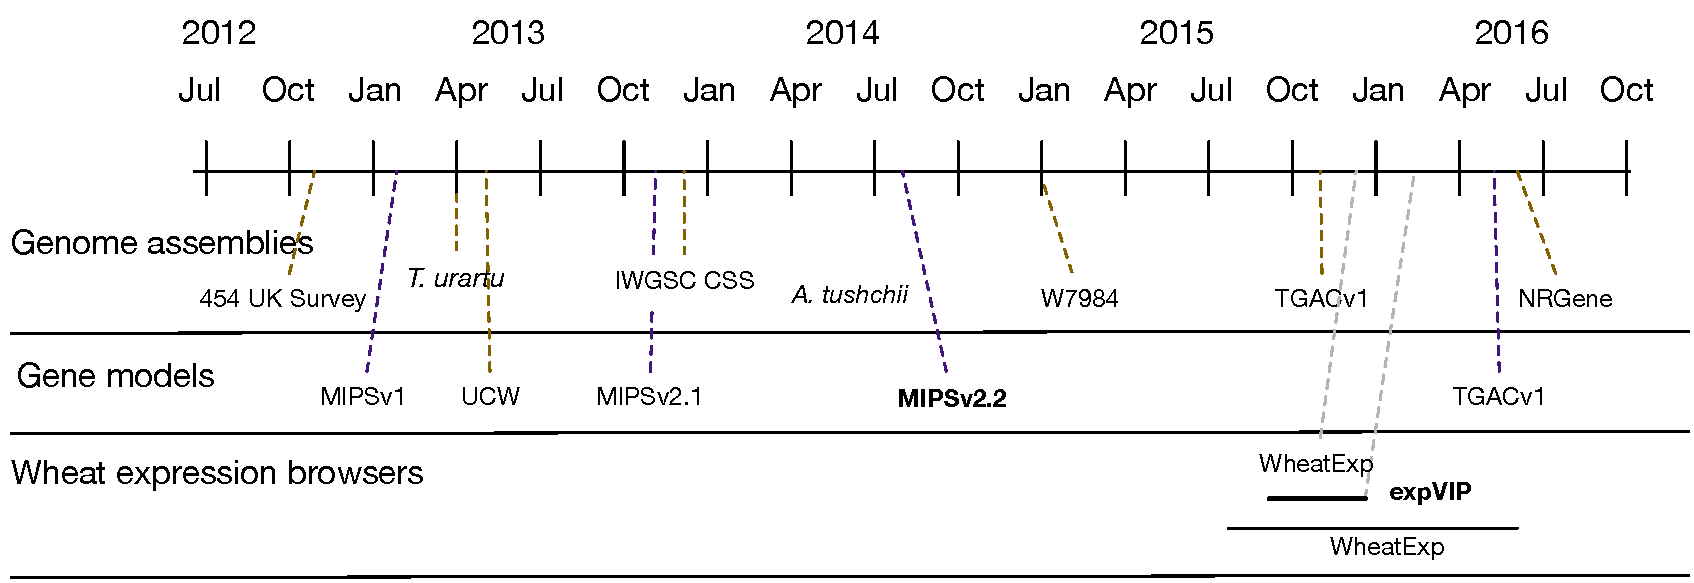
\includegraphics[width=1\textwidth]{expVIP/Figures/Timeline.pdf}
\caption{Timeline of resources used, or potentially used for \gls{yr15}.}
\label{fig:yr15:timeline}
\end{figure}

The quality and completeness  of the reference genome or gene models directly affects the mapping of \gls{ngs} reads. 
This is particularly true on polyploid organisms: if one of the homoeologues is absent, the reads are likely to map to the wrong genome if the parameters of the aligner are relaxed, or not map at all if the required identity is too high.
When the bioinformatic analysis of this project started, the only available wheat genomic reference was a whole genome shotgun 454 sequencing, unassembled \citep{Brenchley2012}; the \gls{css} assembly was being finished \citep{Mayer2014}; the longer scaffolds from \citet{Chapman2015} were not public yet; and finally, the efforts to make a whole genome shotgun assembly were being planned independently by the International Wheat Genome Sequencing consortium  \citep{Pozniak2016} and TGAC (\citealt{Clark2016} ;Figure \ref{fig:yr15:timeline}).  
Because a contiguous assembly with the corresponding annotation was not available at the time of the analysis, and the fact that all the data available was derived from transcriptomic sequencing, the use of gene models as a reference for the alignment was a suitable approach. 

In terms of available gene sets when the analysis started, the canonical reference was the UniGenes from the NCBI \citep{PontiusJUWagnerL2002}. 
The UniGenes are produced with an automated pipeline that clusters all the \glspl{est} deposited in the NCBI by identity and selects the longest transcript, which can merge homoeologous transcripts as a single reference.
Shortly after I started the bioinformatic analysis, two additional gene models were made available, the draft annotation for the \gls{css} assembly (MIPSv1) in January 2013 and the UCW gene models \citep{Krasileva2013} in May 2013. 
I selected the UCW gene models, as they were more mature, phased to distinguish between genomes and already published, over the MIPSv1 genes, as they were still being refined from an initial approach of lifting proteins from related organisms combined with few RNA-Seq experiments.  
The MIPS gene models were improved by removing duplications in the assembly in a later stage and the nomenclature before the release of the assembly \citep{Mayer2014}, but at that point the results of this project had already been submitted for publication (Figure \ref{fig:intro:timeline}; \citealt{Ramirez-Gonzalez2015b}). 
 
To locate the gene models in the chromosome arms and see if there was an enrichment on the called SNPs, the use of a high resolution consensus map is needed, as the genome assemblies available during the analysis are fragmented. 
Initially, I used barley to locate the gene models because the genetic map used to locate the \gls{css} scaffolds was not released yet and barley has a conserved synteny across the wheat genomes. 
The release of a genetic map with over 42,000 markers \citep{Wang2014} was extremely timely, as it happened during the last phase of the project.
Furthermore, as I collaborated in the project, I was also able to use it to locate several \acrshort{css} scaffolds before the release of the assembly. 
The located scaffolds were used as proxy to sort just under half of the reference genes in their chromosomal position (Section \ref{sub:yr15:inSilico}). 
Despite the resolution not being enough to find a single point of enrichment, it was enough to confirm that the SNPs were in the expected location, including one of the SNP candidates flanking the \textit{Yr15} locus (SNP R11, Figure \ref{fig:yr15:BFRValues1BS}).  
If the analysis was to be done today, the genetic map from \citet{Chapman2015} along with their longer scaffolds, or the scaffolds from TGACv1 or the NRGene should provide a better resolution. 
Even without having all the \acrshort{css} scaffolds sorted, the fact that they come from individual chromosome arms enabled the assignment of the genes to a chromosome. 

The original expectation was to have a \gls{nil} for the \gls{bsa} to simplify the SNP discovery and analysis since the majority, if indeed not all of the SNPs should be restricted to the region immediately flanking Yr15. However the number of \glspl{snp} called in the progenitors suggested that the background, \acrlong{avs}, was not the same.  
This happened because despite both susceptible lines being called the same and having the same response to the pathogen, they are in fact different lines from different countries (Section \ref{yr15:snpCalling}). 
This highlights the importance of genotyping the material used when developing mapping populations, especially if the seeds come from different seed banks. 

Despite these shortcomings, the use of the \glspl{bfr} to score the putative SNPs was effective, as most of the SNPs with a high score  mapped in chromosome 1B, in line with previous studies ($BFR>6$, Section \ref{yr15:assaySelection}).
Using the extra criteria of only selecting SNPs from the resistant progenitor and in the expected chromosome arm, I was able to produce a high resolution genetic map (Section \ref{yr15:geneticMap}). 
The genetic map was of the expected resolution for the size of the population (0.26cM on 196 individuals).
Since the mapping population contained only one critical recombinant between \textit{Yr15} and the flanking markers, the population could not yield a better map. 
To improve the map, a cross from the two critical recombinants could be used to repeat a similar analysis, sequencing with either exome capture or RenSeq. 
%\unsure{Talk about Why is R33 diagnostic on the varieties, but maps away?. }

\begin{figure}
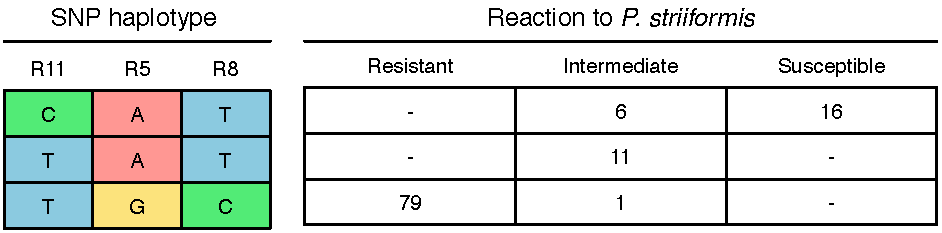
\includegraphics[width=1\textwidth]{Yr15/Figures/breedersTest.pdf}
\caption[Haplotype and phenotype of 113 doubled haploid lines]{Haplotype analysis and phenotypic evaluation of the 113 doubled haploid lines used in the study. The TGC haplotype corresponds to that originally identified in the \textit{Yr15} parent and which was diagnostic across 112 of the 113 lines studied. Figure from \citep{Ramirez-Gonzalez2015b}}
\label{fig:yr15:breeders}
\end{figure}

As described in \citet{Ramirez-Gonzalez2015b}:  
\begin{blockquote} The markers
 R11, R5 and R8 were tested across 122 doubled haploid (DH) lines. 
These DH lines were derived from crosses crosses between five different UK varieties/breeding lines to \textit{Yr15} derivatives known to carry the resistance gene. 
The expected \textit{Yr15} haplotype corresponded to T, G and C alleles at markers R11, R5 and R8, respectively (TGC haplotype). 
The DH lines were tested at seedling stage for reaction to \textit{P. striiformis}, with 84 showing complete resistance and 34 presenting an intermediate or completely susceptible reaction.
The resistant lines all carried the complete \textit{Yr15} haplotype (TGC, Figure \ref{fig:yr15:breeders}) across the three SNP markers with the exception of five lines which had a single missing data point, but were otherwise consistent. 
This compared favourably with the most diagnostic in-house SNP markers available within the breeding programmes. 
Using the three in-house markers, 79 resistant lines carried the expected haplotype, but five completely resistant DH lines were scored as false negative due to the presence of the non-\textit{Yr15} haplotype. 
Within the intermediate and susceptible DH lines, all but one had a non-\textit{Yr15} haplotype (CAT or TAT) across R11, R5 and R8 (Figure \ref{fig:yr15:breeders}). This single DH line was scored as a false positive as it carried the TGC \textit{Yr15} haplotype, but was found to have an intermediate (chlorotic) reaction to \textit{P. striiformis}. This line was also the only one scored as a false positive using the three in-house markers.
\end{blockquote}
%\unsure{This is a very long quote, but I'm finding hard to shorten it. } 
The fact that the developed markers perform better than markers developed by breeders shows the value of this particular experiment and further confirms that \acrshort{bsa} combined with \acrshort{ngs} is an effective way to develop novel markers. 
%\unsure{ Mention other people using a similar strategy since this was published. }

%TODO: Discuss other people using the mark 

In this chapter the integration of different levels of data helped to improve the selection of the candidate SNPs. 
The main criteria for selecting \acrshortpl{snp}  was the\acrshort{bfr} score.
Thanks to the genetic map from \citet{Wang2014} and the \acrshort{css} scaffolds from \citet{Mayer2014}, we were able to confirm that the high scoring \arcshortpl{snp} were in the expected region. 
As the reference genome for wheat improves, defining the location of SNPs linked to a trait of interest will become easier. 
With a continuous reference between two markers flanking a locus and an improved annotation, it will also be possible to compile a more focused set of candidate genes.

%!TEX root = ../Main.tex

\chapter[expVIP]{expVIP: a customisable RNA-seq data analysis and visualisation platform}
\label{cha:exp}

\section{Background.}
Describe the list of previously published expression experiments and how they can potentially be used as a framework for new experiments.  

Co-expression of homoeologus varies from triplet to triplet \citep{Pfeifer2014}
The silencing is mostly regulated by epigenetic changes as the hybridization events are recent.  \citep{Bottley2006}

Kallisto vs sailfish vs tuxedo. 

Table of experiments to include 

The software developed in this section is published in \citep{Borrill2016}. 

\subsection{Relational databases}
A Relational databases is a set of structured tables that have relationships between each other. 
The tables correspond to the data that is essential for the represented concept (domain).
For example, in a table representing several species, the common name and the scientific name belong to the same domain (ie name: Bread wheat; scientific name \textit{Triticum aestivum}). 
Tables in the same relational database form relationships between each other. 
Continuing with the example, an species can have several scientific studies related to them. 
The domain of a study can be formed by the accession, a title, a corresponding manuscript and the species that concerns to it. 
A set of columns that have unique values across the table is called a primary key, in our example an extra \texttt{id} column is added (Figure \ref{fig:expvip:miniER}; \citealt{Codd1970}).
The tables \ref{exp:tab:species} and \ref{exp:tab:studies} have the content of their corresponding domains. 

\begin{figure}
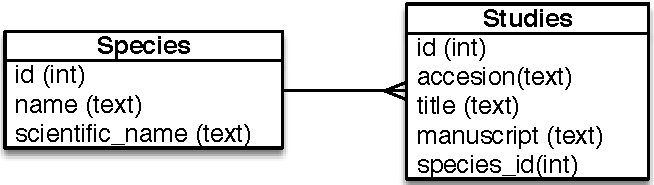
\includegraphics{expVIP/Figures/miniER.pdf}
\caption[Example of a relationship between table.]{Example of a relationship between table. The tables Species and Studies are related. Each study has one species and each species can have several studies.}
\label{fig:expvip:miniER}
\end{figure}

\begin{table}
\caption[Species]{Example content for the table \texttt{species}}
\label{exp:tab:species}
\centering
\begin{tabular}{rll}
\toprule
   id & name                          & scientific\_name                                         \\
\midrule
    1 & Bread wheat                 & Triticum aestivum                                     \\
    2 & Yellow rust                 & Puccinia striiformis              \\
    3 & wheat and rust & T.aestivum,S.tritici  \\
\bottomrule
\end{tabular}

\end{table}

\begin{table}
\caption[Studies]{Example content for the table \texttt{studies}}
\label{exp:tab:studies}
\centering
\begin{tabular}{rllr}
\toprule
   id & accession                                          & manuscript                              &   species\_id \\
\midrule
    1 & DRP000768                                          &  10.1186/1471-2164-14-77          &            1 \\
    2 & ERP003465                                          & 10.1186/1471-2164-14-728            &            1 \\
    3 & ERP004505                                          &  10.1126/science.1250091          &            1 \\
    4 & SRP004884                                          & 10.1186/1471-2164-12-492            &            1 \\
    5 & SRP013449                                          &  10.1111/j.1467-7652.2012.00705.x &            1 \\
    6 & SRP017303                                          & 10.1186/1471-2164-14-270            &            2 \\
    7 & SRP022869                                          &  10.1371/journal.pone.0081606     &            3 \\
\bottomrule
\end{tabular}

\end{table}

\subsection{SQL}
\gls{sql} is a common language to retrieve information from relational databases. 
\acrshort{sql} has operations to select columns and row, join tables, group repeated values and order the results. 
Those simple operations are enough to retrieve the information between tables \citep{Oracle2014}. 
The following list shows a brief description of some commands build a query.  

\begin{description}
\item[\texttt{SELECT <EXPRESSIONS> }]. A list of columns or an expression that will be displayed, separated by commas (\texttt{,}). To display all the columns, the \texttt{*} character represents all the tables. The order of the columns will be the same as the order given in this part of the command
\item[\texttt{FROM <TABLE>}]. follows the column names to add a list of tables to select.
\item[\texttt{JOIN <TABLE> ON <EXPRESSION> }]. is used to join the table from the left side of the statement with the \texttt{<EXPRESSION>} given after the \texttt{ON} clause.  
\item[\texttt{WHERE <EXPRESSION>}] filters the rows by the \texttt{<EXPRESSION>}
\item[\texttt{ORDER BY <COLUMNS>}]. The rows will be sorted by the natural order of the given \texttt{<COLUMNS>}.  
\item[\texttt{GROUP BY <COLUMNS>}]. The rows are merged by the columns stated. This can be used to get an unique set of values and apply a function to all the rows that have the same value, as a count.
\end{description} 

Expressions can be values, operators or functions like:

\begin{description}
\item[\texttt{COLUMN}] The value of a column. 
\item[ \texttt{<EXPRESSION> = <EXPRESSION>}] \texttt{TRUE} when the left and right \texttt{<EXPRESSION>} are equal. \texttt{FALSE} otherwise 
\item[ \texttt{<EXPRESSION> > <EXPRESSION>}] \texttt{TRUE} when the left  \texttt{<EXPRESSION>} is greater than the  right \texttt{<EXPRESSION>} are equal. \texttt{FALSE} otherwise 
\item[ \texttt{<EXPRESSION> < <EXPRESSION>}] \texttt{TRUE} when the left  \texttt{<EXPRESSION>} is less than the  right \texttt{<EXPRESSION>} are equal. \texttt{FALSE} otherwise
\item[ \texttt{COUNT(*)}] The count of rows that have the same values, as selected in the \texttt{GROUP BY} clause.
\end{description}

A simple query to join the  \texttt{species} and \texttt{studies} tables and displaying only the species name, scientific name and accession of the study is shown in Listing \ref{exp:lst:joinExample}. 
The results of the query are in Table \ref{exp:tab:joinExample}. 

\begin{code}[language=sql, label=exp:lst:joinExample,caption=Join example query]
SELECT 
	species.name, 
	species.scientific_name, 
	studies.accession, 
FROM species
JOIN studies on species.id = studies.species_id;
\end{code}

\begin{table}[h!]

\caption[Join example]{Join of the \texttt{species} and \texttt{studies} table. }
\label{exp:tab:joinExample}
\centering
\begin{tabular}{lll}
\toprule
 name                          & scientific\_name                                         & accession                                                                       \\
\midrule
 Bread wheat                 & Triticum aestivum                                     & DRP000768                                          \\ 
 Bread wheat                 & Triticum aestivum                                     & ERP003465                                          \\ 
 Bread wheat                 & Triticum aestivum                                     & ERP004505                                          \\ 
 Bread wheat                 & Triticum aestivum                                     & SRP004884                                          \\ 
 Bread wheat                 & Triticum aestivum                                     & SRP013449                                          \\ 
 Yellow rust                 & Puccinia striiformis            & SRP017303                                          \\ 
 wheat and rust & T.aestivum,S.tritici & SRP022869                                          \\ 
\bottomrule
\end{tabular}

\end{table}


The relationships between tables can be of the following types:

\begin{description}
\item[one-to-one] When rows on a table can be related to a row in a second table. On the diagrams they are represented by a straight line
\item[many-to-many] Rows on a table can have many corresponding rows in a second table, resented with lines with whiskers on both sides of the line.  
\item[one-to-many] Rows on a table can be related to many rows on the second table, represented with whiskers only on one side of the line. 
\end{description}

An important feature of a database is the ability to store the 
data consistently.
A transaction is a set of related operations that need to be performed at the same time.  
To ensure that a transaction needs to follow the principles of \gls{acid} \citep{Haerder1983}.


\begin{description}
\item[Atomicity.] All the operation or none have to be performed. If any of them fails or an error happens while the transaction is executed the data has to be restored to the original status before the transaction started. 
\item[Consistency.] The changes in the database have to be valid before and after the transaction. 
\item[Isolation.] If more than one transaction is being executed at the same time, the result must be the same as if the transactions were executed one after the other. 
\item[Durability.] The result of the transaction is stored even if the server is restarted.
\end{description}  

Several \gls{rdbms} implement \acrshort{sql}, with various levels of compliance to the standard and different licenses.  
A popular \acrshort{rdbms} is \texttt{MySQL}.
From the beginning \texttt{MySQL} aimed to be a lightweight and easy to install open source product \citep{Oracle2014}. 
This characteristics made it popular on the web and it is currently the \gls{rdbms} behind ensembl! \citep{Flicek2012}. 

\subsection{Model-View-Controller}

\begin{SCfigure} 
  \centering
  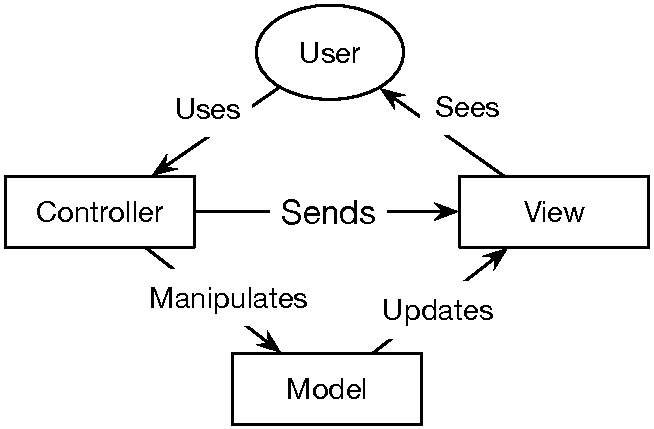
\includegraphics[width=0.7\textwidth]{LitReview/Figures/MVC.pdf}
  \caption{\acrshort{mvc} interaction between components.}
  \label{fig:poly:mvc}
\end{SCfigure}
The \gls{mvc} is a metaphor to isolate the user interactions from the underlying data. 
The models hold the data on logical their domains.
The views contain the layout on how the models are displayed to the user.
The controllers receive the requests from the users and modify the models accordingly and send a view back for display. 
The \acrshort{mvc} metaphor allows the development of independent parts of the system and helps to structure the underlying representation of the domains.  (Figure \ref{fig:poly:mvc}; \citealt{Krasner1988}).

\gls{ror} is a framework to develop web applications heavily influenced by the \acrshort{mvc} metaphor. 
It is based on the Rails language and provides several tasks designed to facilitate the development, such as automated tasks designed to create models with their corresponding views and controllers. 
On the top of that, it provides the tools to manage the connection and queries to the \acrshort{rdbms}, allowing the developer to focus on the functionality \citep{RailsGuide2016}. 

\subsection{Aims}

The aims of expVIP are to:
\begin{enumerate}
\item Integrate RNA-Seq experiments from several sources in a single database (Section \ref{exp:DB}). 
\item Automate the calculation of the expression values and load them in to the database (Section \ref{exp:pipeline}).
\item Produce a visualization for said expression values (Section \ref{exp:gui}).
\item Make the system available to the community (Section \ref{exp:gui}).
\end{enumerate}


\section{General design}

One of the main objectives of expVIP is to make the public expression datasets to the target community (currently wheat, but not limited to it). 
A web interface is an effective is an effective way to reach a global audience. 
A web service requires to have a server to run the application and a browser to connect to the server and display it (ie Internet Explorer, Chrome).
The web server technology used for expVIP is \acrshort{ror}, as it abstracts the \acrshort{mvc} metaphor and it is designed to speed the development \citep{RailsGuide2016}. 
In order to display the expression data to the users, a BioJS component (\citealt{Yachdav2015}, Section \ref{exp:gui}). 
All the data is stored in a MySQL database (Section \ref{exp:DB}) and it is accessed trough models developed under  \acrshort{ror} (Figure \ref{fig:poly:archDesign}).  

\begin{figure} 
  \centering
  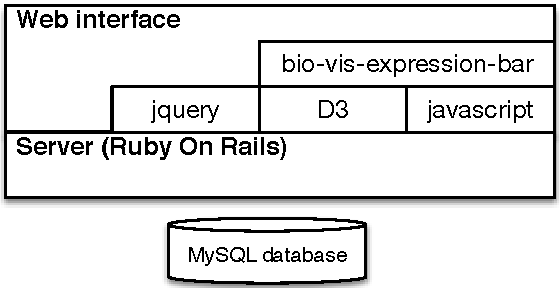
\includegraphics[width=0.9\textwidth]{expVIP/Figures/archDesign.pdf}
  \caption{General design of expVIP}.
  \label{fig:poly:archDesign}
\end{figure}

\section{Database design} 
\label{exp:DB}

To address the different types of conditions over different experiments, expVIP is designed around a relational database. 
The design comprises of two core groups of tables and two auxiliary tables that take care of different species and  homoeologues and (Figure \ref{fig:expvip:dbDesign}).


\begin{sidewaysfigure}
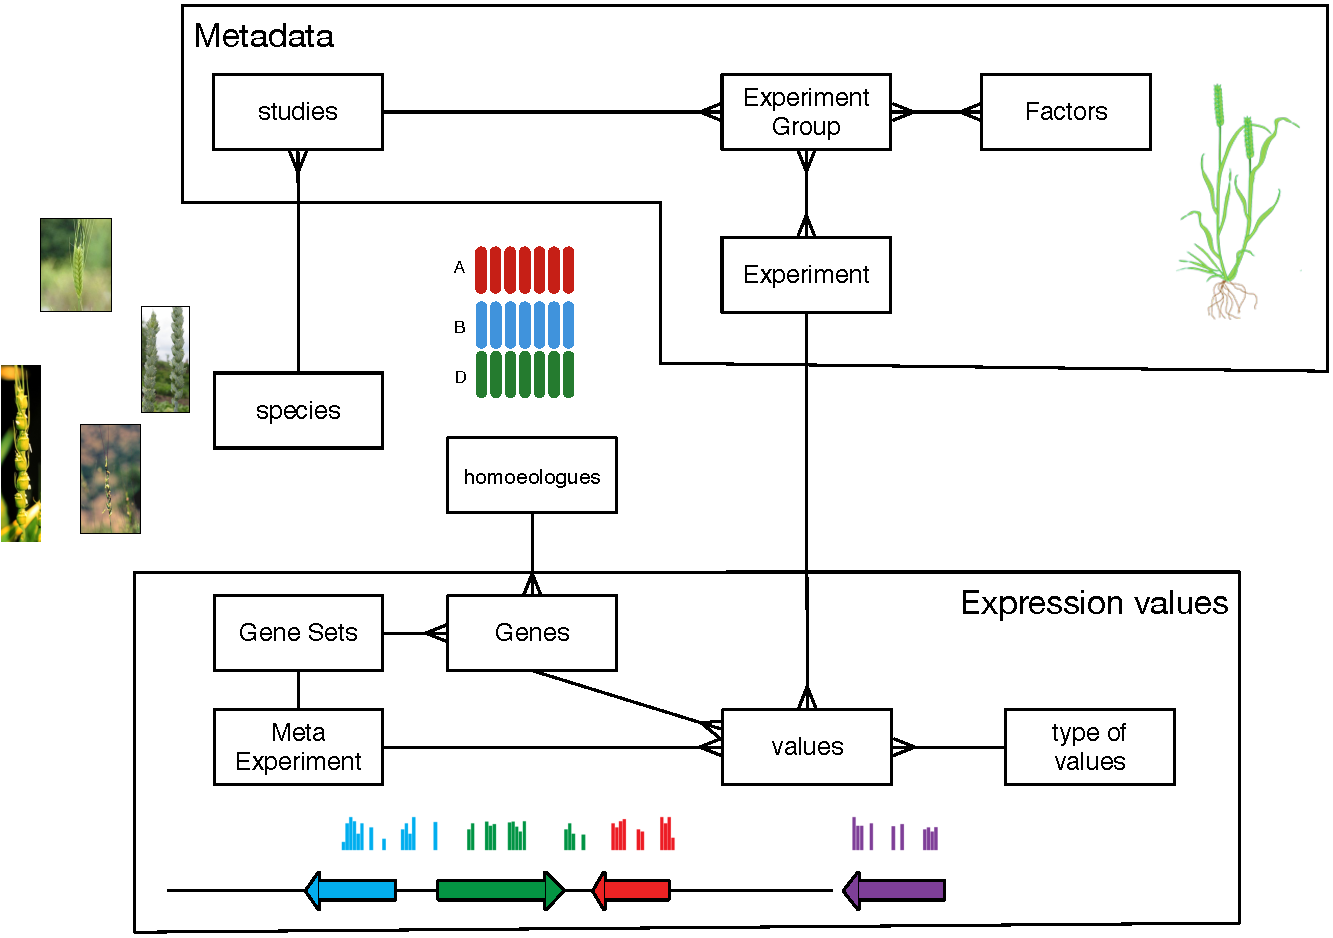
\includegraphics[width=1\textheight]{expVIP/Figures/dbDesign.pdf}
\caption[expVIP database design]{Database design. The block on the top stores the meta-data about the experiments and the studies. The bottom block consist on the tables related to the expression values. Species and homoeologues are outside the main blocks as they are not core to the groups. The whiskers in the connections show the cardinality of the relationships.  }
\label{fig:expvip:dbDesign}
\end{sidewaysfigure}

\begin{description}
\item[Metadata] The tables in this group contain the information of each one of the studies. 
\begin{description}
\item[Studies] Contains the general information of a study, which contain several experiments. The table also contains the reference to the paper where the data is published and the accession for the study. 
\item[Experiment group] keeps together all the individual experiments that come from the same study and that were taken on the same condition (ie. replicates). 
\item[Factors] holds all the possible factors used to group the experiments. Each experiment group has many factors and each factor group has many experiment groups. As the experiment doesn't have a fixed number of column representing each factor, it is possible to have any arbitrary number factors to group. 
\item[Experiment] holds the information of each individual experiment, with the corresponding accession. 
\end{description}
\item[Expression values.] The tables on this block contain the expression of each gene and the information for the genes. 
\begin{description}
\item[Types of value] keeps a list of different units that are stored. On the original design \acrshort{tpm} and raw counts are set up, but as the units are not hard coded it is possible to use \acrshort{fpkm}, \acrshort{rpkm} or, any other unit. 
\item[Gene Set] contains the name of a reference gene set for the analysis. On the original version of expVIP, the gene models from the \acrshort{iwgsc} as deposited in Ensembl release 26 were used \citep{Mayer2014} However, the use of this table enable the use of several reference gene models on the same database. 
\item[Genes] are related to a \texttt{gene set}, so even if they have the same name coming from different datasets it is possible to distinguish them. This situation is unlikely to occur when using published references, but when joining several \textit{de Novo} gene models. 
\item[Meta Experiment] allows to have the same data analysed with different tools. By default expVIP uses Kallisto \citep{Bray2016}. However other tools, or different versions of the same tool, can be used to repeat the analysis.   
\item[Values] have a domain that includes the \texttt{meta experiment}, \texttt{gene} and, \texttt{type of value}.
\end{description}
\item[Homoeologues] contain the relationship between genes. This allows to get the expression values of several related genes. 
\item[Species] contain the target species of a study. It is not linked to the gene models to allow the direct comparison between related species using the same gene models (ie, \texttt{T. aestivum} vs \texttt{T. turgidum}). 
\end{description}

In the cases that a relationship between tables is not unique, such as \texttt{experiment\_groups} having many \texttt{factors} and the \texttt{factors} having many \texttt{experiment\_groups}, storing the relationships is done with an auxiliary table (ie. \texttt{ExperimentGroups\_Factors}, not explicitly shown in Figure \ref{fig:expvip:dbDesign}, but implicit by the lines with whiskers). 

%The database is designed to be flexible to accommodate users using non-model organisms were the available resources may be limited. 

Once all the data is stored, the tables can be queried together to make clear the relationship between specific rows. 
One of the core tasks of expVIP is to get all the factors that define each experiment, in order to be able to merge similar studies. 
To retrieve the \texttt{experiments} and \texttt{factors} of an \texttt{experiment group}, the auxiliary tables \texttt{ExperimentGroups\_Factors}  and \texttt{experiment\_groups\_experiments} are used in the query. (Listing \ref{lst:exp:queryMetadata} and Table \ref{tab:exp:queryMetadata}).


\begin{code}[language=sql, caption={[Query experiments and factors]Query experiments and factorsQuery experiments and factors from accession 'DRR003148'},label=lst:exp:queryMetadata]
SELECT
	experiments.accession,  
	factors.factor,
	factors.description, 
	experiment_groups.name as expriment_group 
FROM factors 
JOIN ExperimentGroups_Factors 
	ON factors.id = ExperimentGroups_Factors.factor_id
JOIN experiment_groups 
	ON experiment_groups.id = ExperimentGroups_Factors.experiment_group_id
JOIN experiment_groups_experiments 
	ON experiment_groups_experiments.experiment_group_id = experiment_groups.id
JOIN experiments 
	ON experiments.id = experiment_groups_experiments.experiment_id
WHERE accession =  'DRR003148'
\end{code}

%\pagebreak
\begin{table}[h]
\caption[Results of query for metadata]{Results of querying the metadata for accession 'DRR003148' (Listing \ref{lst:exp:queryMetadata})}
\label{tab:exp:queryMetadata}
\begin{tabular}{llll}
\toprule
 accession   & factor                    & description    & expriment   \\
     &                     &     & group   \\
\midrule
 DRR003148   & Age                       & 24 days        & Group1            \\
 DRR003148   & High level age            & vegetative     & Group1            \\
 DRR003148   & High level stress-disease & no stress      & Group1            \\
 DRR003148   & High level tissue         & roots          & Group1            \\
 DRR003148   & High level variety        & Chinese Spring & Group1            \\
 DRR003148   & Stress-disease            & none           & Group1            \\
 DRR003148   & Tissue                    & roots          & Group1            \\
 DRR003148   & Variety                   & Chinese Spring & Group1            \\
\bottomrule
\end{tabular}

\end{table}

Likewise, to get the \texttt{expression\_values} for a \texttt{gene} with the corresponding unit (\texttt{type\_of\_values}) and \texttt{experiment} a simple query joining the four tables is used. 
The Listing \ref{lst:exp:queryExpValues} retrieves the \texttt{expression\_values} for the \texttt{gene} 'Traes\_5BS\_0AFC3F795.1', and the result is on Listing \ref{tab:exp:queryExpValues}

\begin{code}[language=sql, caption={[Query values for gene and experiment group] Query values from 'Group1' and gene 'Traes\_5BS\_0AFC3F795.1' },label=lst:exp:queryExpValues]
SELECT 
	genes.name as gene, 
	expression_values.value,
	experiments.accession,
	type_of_values.name as unit
FROM expression_values
JOIN genes 
	ON expression_values.gene_id = genes.id
JOIN type_of_values 
	ON type_of_values.id = expression_values.type_of_value_id
JOIN experiments 
	ON experiments.id = expression_values.experiment_id
WHERE 
	genes.name = 'Traes_5BS_0AFC3F795.1' 
\end{code}

\begin{table}[h]
\caption[Results of query for values]{Results of query to get the values for gene 'Traes\_5BS\_0AFC3F795.1' (Listing \ref{lst:exp:queryExpValues}), only 'Group1' is displayed from the output.}
\label{tab:exp:queryExpValues}
\begin{tabular}{lrlll}
\toprule
 gene                  &    value & accession   & experiment   & unit   \\
                    &     &    & group   &    \\
\midrule
 Traes\_5BS\_0AFC3F795.1 & 136.995  & DRR003148   & Group1             & count  \\
 Traes\_5BS\_0AFC3F795.1 & 120.683  & DRR003149   & Group1             & count  \\
 Traes\_5BS\_0AFC3F795.1 & 140.94   & DRR003150   & Group1             & count  \\
 Traes\_5BS\_0AFC3F795.1 &  24.2277 & DRR003148   & Group1             & tpm    \\
 Traes\_5BS\_0AFC3F795.1 &  23.9739 & DRR003149   & Group1             & tpm    \\
 Traes\_5BS\_0AFC3F795.1 &  24.9835 & DRR003150   & Group1             & tpm    \\
\bottomrule
\end{tabular}

\end{table}

With those two queries is enough to retrieve all the information required to do sub-groupings. 

The database is implemented using the \acrshort{rdbms} \texttt{MySQL 5.5}. 



\section{Data integration pipeline} 
\label{exp:pipeline}


To prepare the database, expVIP requires to have all the metadata for the experiments to integrate. 
ExpVIP contains tasks to load all the metadata and a wrapper for Kallisto that can be run from expVIP. 
Alternatively, the expression values can be calculated with another tool and loaded as a single file, this approach is preferred for a large set of samples (Figure \ref{fig:exp:loadPipeline}). 
Details on how to load the files in the database are in the expVIP tutorial (Appendix \ref{exp:tutorial}). 

\begin{figure}
\centering
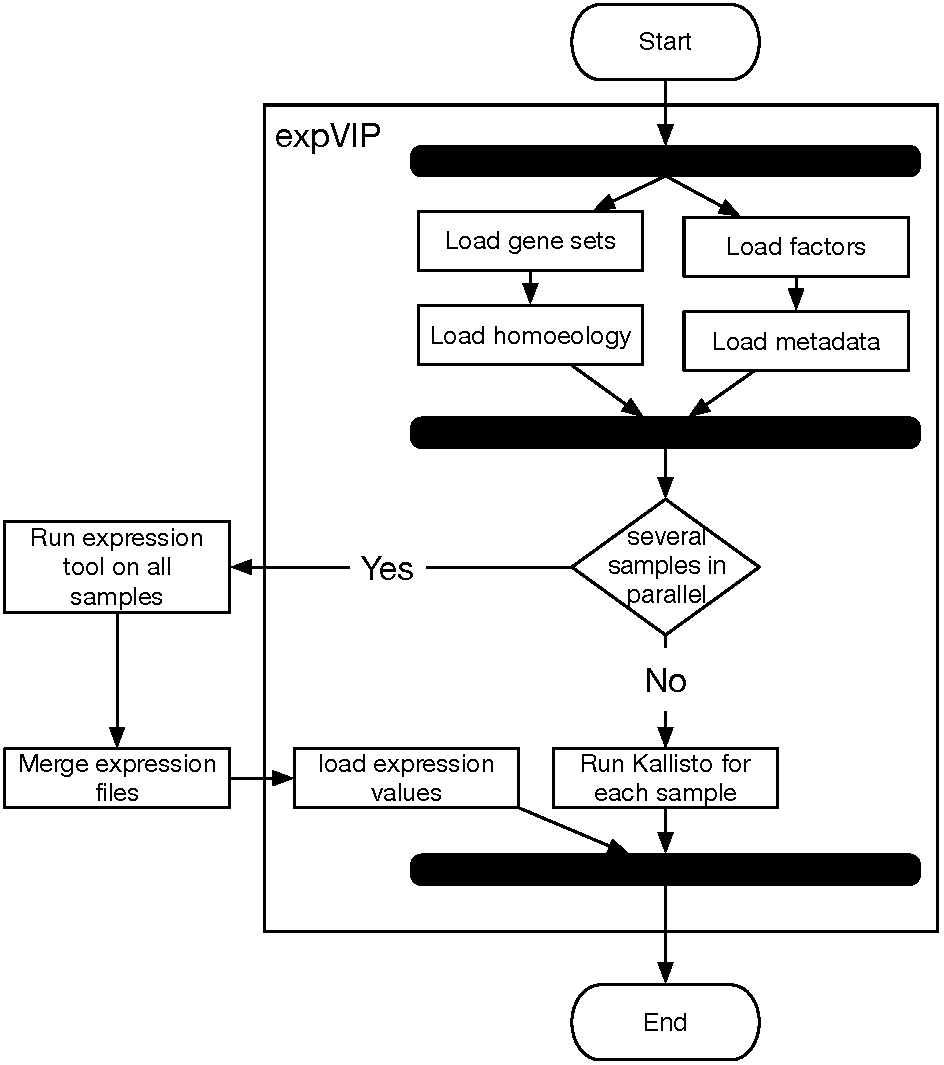
\includegraphics[width=1\textwidth]{expVIP/Figures/loadDataPipeline.pdf}
\caption[expVIP load data]{The pipeline of loading the data to expVIP. The black lines represent a border of tasks that can be run in parallel or don't require to be done in a particular order.}
\label{fig:exp:loadPipeline}
\end{figure}

The required files for the metadata are:
\begin{description}
\item[Factors.] The file contains all the possible factors that can be used to group all the experiments. The file must contain the following columns (Table \ref{tab:exp:factors}):
\begin{description}
\item[factor] The category were the factor belongs. In the case of the initial dataset used in expVIP, the grouping factors are: Age, stress-disease, tissue and, a corresponding 'High level' for each factor. The metadata file must contain a cloumn corresponding to each one of this factors. 
\item[order] The default order in which to display each factor. This ensures that the age of the plants are sorted chronologically. 
\item[name] Long description of each factor. This are used as valid values in the metadata.  
\item[short] Is a short name, used when the space to display the full description of the factor is not enough.
\end{description}
\begin{table}
\centering
\caption[Factors file]{Factors file. The table must be saved as a text file, with columns separated by tabs}
\label{tab:exp:factors}
\begin{tabular}{llll}
\toprule
factor & order & name & short \\
\midrule
Age & 1 & 7 days & 7d \\
Age & 2 & seedling stage & see \\
Age & 3 & 14 days & 14d \\
Age & 4 & three leaf stage & 3\_lea \\
Age & 5 & 24 days & 24d \\
High level age & 1 & seedling & see \\
High level age & 2 & vegetative & veg \\
High level age & 3 & reproductive & repr \\
High level stress-disease & 1 & none & none \\
High level stress-disease & 2 & disease & dis \\
High level stress-disease & 3 & abiotic & abio \\
High level stress-disease & 4 & transgenic & trans \\
High level tissue & 1 & spike & spike \\
High level tissue & 2 & grain & grain \\
... & & \\
\bottomrule
\end{tabular}
\end{table}
\item[metadata] The metadata file is the file that contains the information related to each study and the corresponding experiments. 
Each study contains several experiment groups (replicates), which in turn contain every individual experiment. 
The factors must be shared across experimental groups. 
\begin{description}
\item[secondary\_study\_accession] The accession number for experiments carried as part of a single study. This is usually the high level BioProject or SRA number. 
\item[run\_accession] The accession of the individual run. 
\item[scientific\_name] of the species. 
\item[experiment\_title] A description for the individual RNA-seq sample.
\item[study\_title] A description of the general study.
\item[Manuscript] The DOI of the study.
\item[Group\_for\_averaging] A description of the experiment. This must be the same all the replicates in the same study. 
\item[Group\_number\_for\_averaging] A short name for replicated experiments.  
\item[Total reads] (optional)
\item[Mapped reads] (optional)
\end{description}
Besides the main fields, each factor has a a corresponding column Variety, Tissue,Age, Stress-disease, High level variety, High level tissue, High level age and, High level stress-disease

\item[Gene set] The gene set is provided as a single fasta file. 
The file may contain alternative transcripts from the same gene. To identify this, the fasta header may include the optional fields \texttt{gene} and \texttt{transcript}. 
On the absence of this, the only stored value is the name from the \textgreater  character to the first space (Listing \ref{lst:poly:geneFa}). 

\begin{code}[label=lst:poly:geneFa, caption={[Gene set fasta file] A fasta entry on of the gene set.}]
>Traes_5BL_3FC5BA305.1 cdna:novel scaffold:IWGSC2:IWGSC_CSS_5BL_scaff_1082268:5:199:-1 gene:Traes_5BL_3FC5BA305 transcript:Traes_5BL_3FC5BA305.1
TGCTGCTGCTAGGCTTGAAGAGGTTGCTGGCAAGCTCCAGTCTGCTC
GGCAGCTCATTCAGAGGGGCTGTGAGGAGTGCCCCAAGAACGAGGAT
GTTTGGTTCGAGGCATGCCGGTTGGCTAGCCCAGATGAGTCAAAGGC
AGTAATTGCCAGGGGTGTGAAGGCAATTCCCAACTCTGTGAAGCTGT
GGCTGCA
\end{code}
\item[homoeologues] A file containing the homoeologues for the  A, B and D genomes. Currently this are the only supported default names. The file also include a column with the gene name and to which Group (ie 1, 2, 3 ... 7) and Genome (ie A, B or D) it belongs (Table \ref{tab:exp:hom}).  

\begin{sidewaystable}
\centering
\caption[Homoeology file]{Example tabular file containing the homoeology across the three genomes. }
\label{tab:exp:hom}
\begin{tabular}{llllll}
\toprule
Gene & A & B & D & Group & Genome \\
\midrule
Traes\_5BS\_0AFC3F795 & Traes\_5BS\_0AFC3F795 & Traes\_5BS\_0AFC3F795 & Traes\_5DS\_C204EBAA9 & 5 & B \\
Traes\_5DS\_C204EBAA9 & Traes\_5DS\_C204EBAA9 & Traes\_5BS\_0AFC3F795 & Traes\_5DS\_C204EBAA9 & 5 & D \\
Traes\_7DL\_82360D4EE1 & Traes\_7DL\_82360D4EE1 & Traes\_7DL\_82360D4EE1 & & 7 & D \\
Traes\_2AL\_1368BE0AD & & Traes\_2AL\_1368BE0AD & Traes\_2BL\_CD459994C1 & 2 & A \\
... & & & & &  \\
\bottomrule 
\end{tabular}
\end{sidewaystable}
\end{description} 

expVIP includes several tasks to load the different files. 
For example, to load the factors the \verb|load_data:factor| starts a transaction (Listing \ref{lst:exp:laodFactor}; line 2) to ensure that all the data is loaded, and if for some reason the load fails, the database is restored to the previous status.
In the transaction, the file is open with the \verb|csv| library row by row (line 3).
The function \verb|find_or_create_by| is a function that \acrshort{ror} provides on models to create an entry in the table, or update it if already exists.
Each row is used to create or update a \verb|Factor| (lines 374-376). 
A similar strategy is used for all the files that are regular tables. 

\begin{code}[language=ruby, caption={[Load factors]Task that loads factors}, label=lst:exp:laodFactor]
task :factor, [:filename] => :environment do |t, args|
  ActiveRecord::Base.transaction do 
    CSV.foreach(args[:filename], :headers => true, :col_sep => "\t") do |row|
      factor = Factor.find_or_create_by(:factor=>row["factor"],  :description=>row["name"],  :name=>row["short"])
      factor.order = row["order"].to_i
      factor.save!
    end
  end
end
\end{code}

The gene sets are loaded slightly differently, as the input is a \verb|fasta| file, as opposed to tabular file. 
The reader for the \verb|FastaFormat| from BioRuby \citep{Goto2010} is used to read the file (Listing \ref{lst:exp:loadGenes}; line 4). 
Since expVIP only records the name of the genes, only the id of the fasta sequence is extracted (lines 6-79). 
The name is stored in the name and cDNA columns. 
The parser for entries from ensembl, such the one in Listing \ref{lst:poly:geneFa} include code to load the cdna and transcript fields correctly. 

\begin{code}[language=ruby, caption={[Load genes from Fasta]Task that load genes from a Fasta File}, label=lst:exp:loadGenes]
task :de_novo_genes, [:gene_set,:filename] => :environment do |t, args|
  ActiveRecord::Base.transaction do
    gene_set = GeneSet.find_or_create_by(:name=>args[:gene_set])
    Bio::FlatFile.open(Bio::FastaFormat, args[:filename]) do |ff|
      ff.each do |entry| 
        arr = entry.definition.split(/\s+/)
        name = arr[0]
        g = Gene.new 
        g.gene_set = gene_set
        g.name = name
        g.cdna = name
        g.save!
      end
    end
  end
end
\end{code}


\section{Graphical interface}
\label{exp:gui}  
How the expression can be displayed filtered, and sorted

%%\section{Virtual Machine}
%%\label{exp:vm}
\unsure{If I have time, I'll add the section about the virtual machine, as I would also need to add something in the background on virtualisation, it can potentially be a sink of time}

\section{Discussion} 
The use of previously published studies is a valuable resource. Also, mention that despite the fact that there are several expression/gene browsers, none of them allow comparisons between species and don't consider polyploids. 

Things to do: add comparassions between corresponding genes between species
%!TEX root = ../Main.tex

\chapter{General discussion and final remarks}
%This section wraps up by showing the relationship and importance of a comprehensive approach to data analysis, from the field, genetics, molecular biology and genomics. I will also remark how the technology and the resources have changed in the last 4 years. As at the references used at beginning where superseded during the PhD. 

%Biology is becoming interdisciplinary

\section{Biology as an interdiciplinary science}

Knowledge from  computer science can be applied to produce software for specific needs, but useful for the comunity

Polyploidy has an extra level of complexity (due to homoeologues), but with the current developments of technology is possible to start getting around them. 



In the case of wheat, new resources had been coming out year after year, and each one helps to put everything in to a context. 

With the plethora of information currently available (See section \ref{lit:wheatResourcers}), it is possible to 


In Chapter \ref{yr15} the integration of different levels of data helped to improve the selection of the candidate SNPs. 
The main criteria for selecting \acrshortpl{snp}  was the\acrshort{bfr} score.
However, thanks to the genetic map from \citet{Wang2014} and the \acrshort{css} scaffolds \citep{Mayer2014}) enabled to confirm that the high scores were in the expected region. 
As the reference genome for wheat improves, the location of SNPs linked to a trait will be easier. 
With a continous reference between two markers flanking a locus and an improve annotation, a more focused set of gene candidates will be possible. 

%However, in the case of introgressions a good reference genome may not be enough to find a gene candidate. 
%This is because the gene may come from a region significantly different to the

\section{The right reference}

The efforts to produce a wheat reference genome had been focused on the \gls{cs} variety. 
\acrshort{cs} is only cultivated as a research line, as it is susceptible to several pathogens and its yield is inferior to modern varieties.  
The reason for \acrshort{cs} to be the selected cultivar to be sequenced as reference is historic: it has long been a variety  for resarch.
\acrshort{cs} was originally picked because it was able to cross with rye. 
It has also been used to produce lines with chromosomic aberrations, useful to find if any particular chromosome is responsible for certain traits \citep{Sears1985}. 


%It is more likely to get relevant results in a more effective way using the latest developments. 


\section{A database to put integrate all the resources. }

\begin{sidewaysfigure}
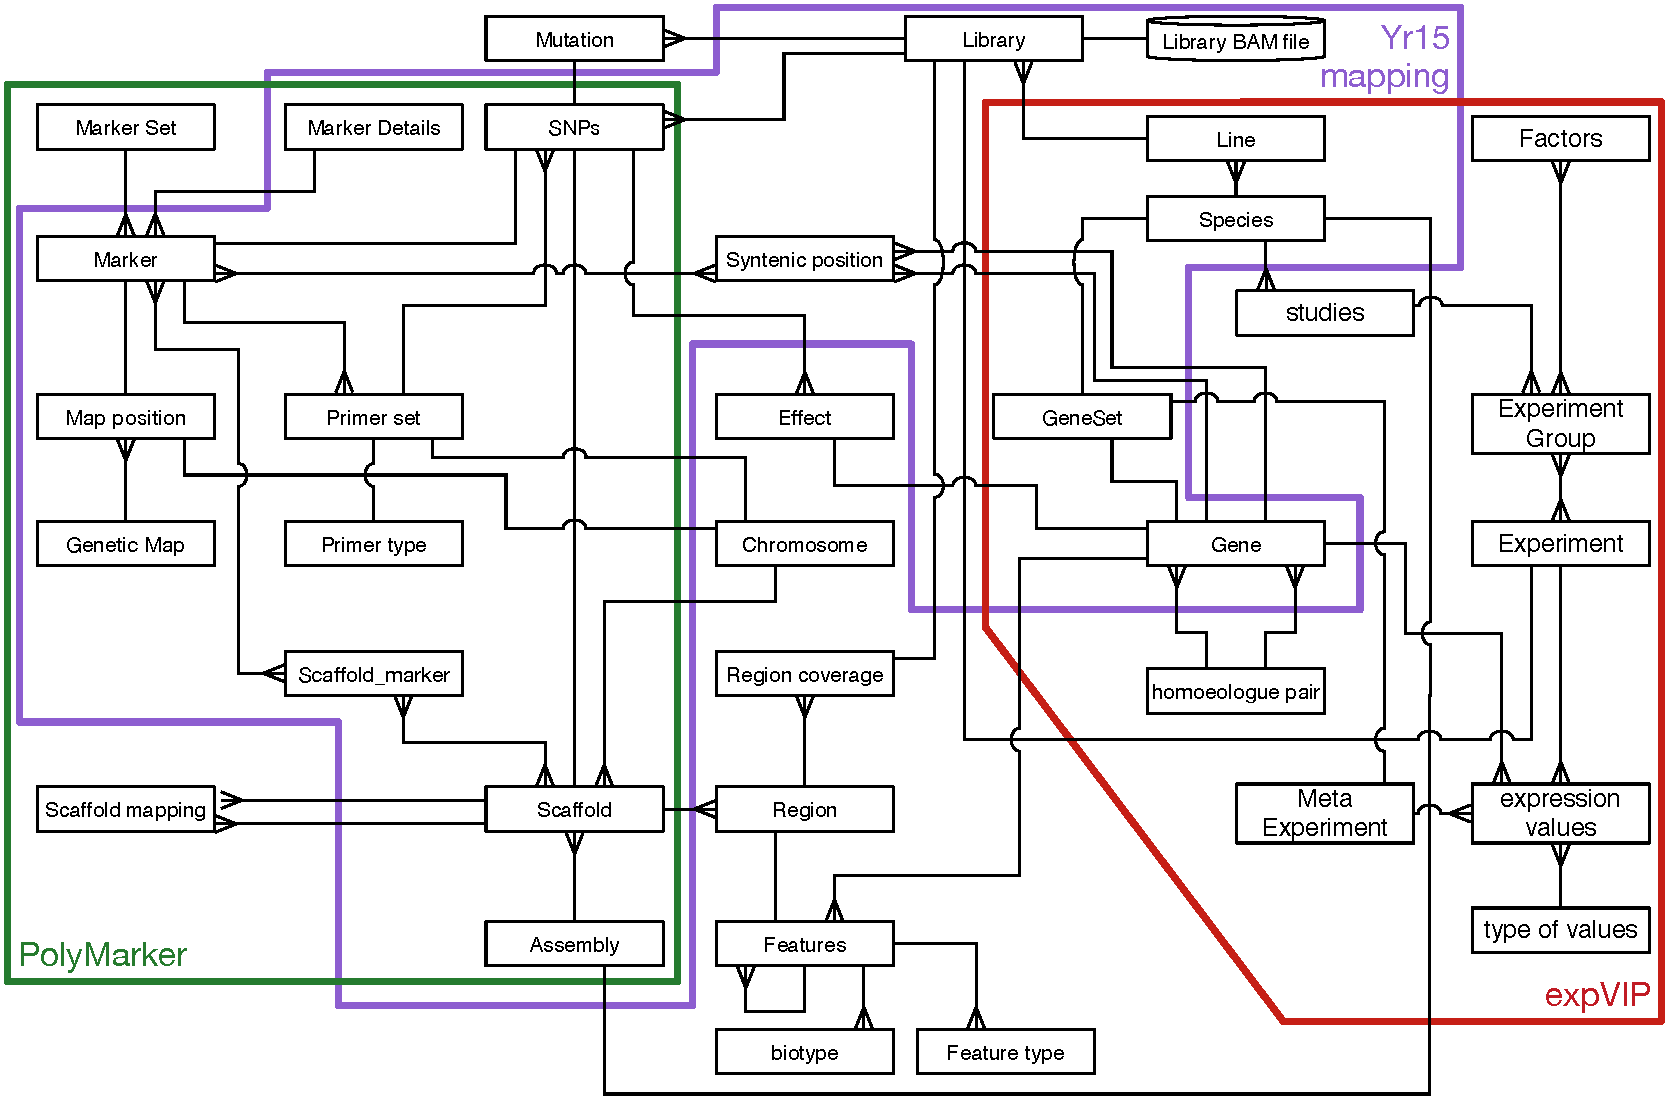
\includegraphics[width=1\textwidth]{Conclusions/Figures/CompleteDatabase.pdf}
\caption{Database integrating all the datasets}
\end{sidewaysfigure}
Integration of the different datasets as used in the project. 
Make the point of the use a GFF File. 

\section{Integration with other services}
Currently, the publicly available wheat resources are scattered as supplemental materials on their corresponding publication or available as ad hoc systems focused on a particular field.
For example ensembl has two different views for every organism: from the genomic point of view and from the expression data. 
The Collaborative Open Plant Omics (COPO; \citealt{Davey2015}) is trying to integrate different sources and types of data by connecting the data providers. 
This approach requires the cooperation of the service providers, which have their own view of what is important. 
I believe that in order to effectively integrate the resources it is necessary to understand how the users are likely to interact with the data.

\section{Side projects}

PolyInDel / . 





\appendix
\chapter{Supplemental tables}
%!TEX root = ../Main.tex

\section{Genetic map of \textit{Yr15} with RNA-Seq supplemental tables.}

%!TEX root = ../../Main.tex
\begin{sidewaystable}
\centering
\caption{Number of genes with a coverage over 20x, 10x and at least one read (\ensuremath{>}0x). }
\label{app:seqAlnCov}
\begin{localsize}{10}{11}

\begin{tabular}{llrrrrrr|rrrr|rr}
\toprule
          &             & \multicolumn{6}{c}{Bulks} & \multicolumn{4}{c}{Bulk  mixes} & \multicolumn{2}{c}{Progenitors}        \\
 Coverage & Reference   & R1     & R2     & R3     & S1     & S2     & S3     & R1+R2       & S1+S2  & R1+R2+R3 & S1+S2+S3 & \textit{Yr15}        & AVS     \\
 \midrule
 20x      & UCW         & 16,434 & 27,871 & 27,223 & 32,287 & 28,669 & 34,898 & 33,968      & 41,019 & 40,985   & 47,507   & 36,808      & 42,248  \\
          &             & 17\%    & 30\%    & 29\%    & 34\%    & 30\%    & 37\%    & 36\%         & 44\%    & 44\%      & 50\%      & 39\%         & 45\%     \\
          & UniGene v60 & 9,643  & 16,182 & 15,222 & 19,549 & 17,397 & 20,567 & 20,219      & 25,270 & 24,598   & 29,052   & 22,107      & 25,842  \\
          &             & 17\%    & 28\%    & 27\%    & 34\%    & 31\%    & 36\%    & 36\%         & 44\%    & 43\%      & 51\%      & 39\%         & 45\%     \\
 \midrule
 10x      & UCW         & 27,371 & 38,282 & 37,777 & 42,658 & 38,999 & 44,610 & 43,266      & 49,473 & 49,182   & 54,781   & 46,356      & 50,760  \\
          &             & 29\%    & 41\%    & 40\%    & 45\%    & 41\%    & 47\%    & 46\%         & 53\%    & 52\%      & 58\%      & 49\%         & 54\%     \\
          & UniGene v60 & 16,201 & 22,948 & 22,130 & 26,200 & 24,130 & 26,914 & 26,318      & 30,579 & 29,857   & 33,557   & 28,044      & 31,095  \\
          &             & 28\%    & 40\%    & 39\%    & 46\%    & 42\%    & 47\%    & 46\%         & 54\%    & 52\%      & 59\%      & 49\%         & 55\%     \\
 \midrule
 \ensuremath{>}0x      & UCW         & 68,302 & 72,484 & 72,957 & 74,694 & 73,290 & 75,201 & 74,397      & 77,093 & 76,715   & 78,796   & 76,275      & 77,080  \\
          &             & 73\%    & 77\%    & 77\%    & 79\%    & 78\%    & 80\%    & 79\%         & 82\%    & 81\%      & 84\%      & 81\%         & 82\%     \\
          & UniGene v60 & 40,717 & 42,489 & 42,595 & 43,625 & 43,059 & 43,748 & 43,393      & 44,655 & 44,364   & 45,392   & 43,732      & 44,596" \\
          &             & 71\%    & 75\%    & 75\%    & 77\%    & 76\%    & 77\%    & 76\%         & 78\%    & 78\%      & 80\%      & 77\%         & 78\%     \\
\bottomrule
\end{tabular}

\end{localsize}
\end{sidewaystable}



%
\begin{sidewaystable}
\centering
\caption{PolyMarker used to genotype PST. The X and Y represent the the two possible allels.  X:X and Y:Y correspond to homozygous call of the corresponding allele. X:Y correspond to heterozygous calls. The '-' symbol correspond to failed assays. }
\label{app:PolyMarkerPST}
\begin{localsize}{9}{10}

\begin{tabular}{rlrll|cc|cc|ccc|cc}
\toprule
          &              &  &  & & \multicolumn{2}{c}{Cluster I isolates}        & \multicolumn{2}{c}{Cluster II isolates}        & \multicolumn{3}{c}{Cluster III isolates}         & \multicolumn{2}{c}{Cluster IV isolates}        \\
Assay & Contig       & Position &  X &  Y & 13/26              & 13/123 & CL1                 & T-13/3 & 13/09                & 13/23 & 13/182 & 13/36               & 13/40 \\
 \midrule
  1  & PST130\_14470 & 268      & C        & T        & X:Y                & X:Y    & X:X                 & X:X    & X:X                  & X:X   & X:X    & X:X                 & X:X   \\
  2  & PST130\_8160  & 11876    & C        & T        & Y:Y                & Y:Y    & X:Y                 & X:Y    & X:Y                  & X:Y   & X:Y    & X:Y                 & X:Y   \\
  3  & PST130\_14628 & 1712     & A        & C        & X:Y                & -      & X:X                 & X:X    & X:X                  & X:X   & X:X    & X:X                 & X:X   \\
  4  & PST130\_14898 & 503      & G        & A        & X:X                & X:X    & X:Y                 & X:Y    & X:Y                  & X:Y   & -      & X:Y                 & X:Y   \\
  5  & PST130\_28344 & 2372     & A        & G        & Y:Y                & Y:Y    & X:Y                 & X:Y    & Y:Y                  & Y:Y   & Y:Y    & Y:Y                 & Y:Y   \\
  6  & PST130\_7634  & 3463     & A        & C        & Y:Y                & Y:Y    & X:Y                 & X:Y    & Y:Y                  & Y:Y   & Y:Y    & Y:Y                 & Y:Y   \\
  7  & PST130\_7629  & 11699    & G        & A        & Y:Y                & Y:Y    & X:Y                 & X:Y    & Y:Y                  & Y:Y   & Y:Y    & Y:Y                 & Y:Y   \\
  8  & PST130\_10943 & 2979     & C        & T        & X:Y                & X:Y    & X:Y                 & X:Y    & X:X                  & X:X   & X:X    & X:Y                 & X:Y   \\
  9  & PST130\_10126 & 6216     & G        & T        & Y:Y                & Y:Y    & X:X                 & X:X    & X:X                  & X:X   & -      & Y:Y                 & Y:Y   \\
  10 & PST130\_22010 & 172      & C        & T        & Y:Y                & Y:Y    & Y:Y                 & Y:Y    & X:Y                  & X:Y   & -      & X:Y                 & X:Y   \\
  11 & PST130\_16961 & 1098     & C        & T        & X:X                & X:X    & X:Y                 & X:Y    & Y:Y                  & Y:Y   & Y:Y    & X:Y                 & X:Y   \\
  12 & PST130\_6915  & 2710     & A        & T        & Y:Y                & Y:Y    & Y:Y                 & Y:Y    & Y:Y                  & X:Y   & X:Y    & Y:Y                 & Y:Y   \\
  13 & PST130\_12479 & 1428     & C        & T        & X:X                & X:X    & Y:Y                 & Y:Y    & X:X                  & X:X   & X:X    & Y:Y                 & X:X   \\
  14 & PST130\_7634  & 3883     & C        & G        & X:X                & X:X    & X:Y                 & X:Y    & X:X                  & X:X   & X:Y    & X:Y                 & X:X   \\
  15 & PST130\_14470 & 456      & T        & C        & Y:Y                & Y:Y    & X:Y                 & X:Y    & Y:Y                  & Y:Y   & X:Y    & Y:Y                 & Y:Y   \\
\bottomrule
\end{tabular}
\end{localsize}
\end{sidewaystable}


%\begin{sidewaystable}
\centering
\caption{Validation of homozygous deletions on line Cadenza0423. }
\label{app:poly:homDelCad0423}
\begin{localsize}{6}{7}
\begin{tabular}{llllrllllllllllllllll}
\toprule
 Marker                                   & Deletion           & chr   &     cM & 1   & 2   & 3   & 4   & 5   & 6   & 7   & 8   & 9   & 10   & 11   & 12   & C   & C   & C   & C   & Result       \\
\midrule
 5BS\_2297308\_Cadenza0423\_12664\_C12664T    & -          & 5B    &  4.551 &  X   & X   & -   & X   & X   & X   & X   & X   & X   & X    & -    & X    & Y   & Y   & Y   & Y   & HOM Mutation \\
 5BL\_10812849\_Cadenza0423\_5664\_G5664T     & -          & 5B    & 38.769 &  X   & X   & -   & X   & X   & X   & X   & X   & X   & X    & -    & X    & Y   & Y   & Y   & Y   & HOM Mutation \\
 5BL\_10825062\_Cadenza0423\_7917\_G7917A     & -          & 5B    & 38.769 &  X   & X   & -   & X   & X   & X   & X   & X   & X   & X    & -    & X    & Y   & Y   & Y   & Y   & HOM Mutation \\
 IWGSC\_CSS\_5BL\_scaff\_10847976:27068-27231 & +          & 5B    & 38.769 &  X   & X   & -   & X   & X   & X   & X   & X   & X   & X    & -    & X    & H   & H   & H   & H   & Hom Deletion \\
 IWGSC\_CSS\_5BL\_scaff\_10847976:28118-28674 & +          & 5B    & 38.769 &  X   & X   & -   & X   & X   & X   & X   & X   & X   & X    & -    & X    & H   & H   & H   & H   & Hom Deletion \\
 IWGSC\_CSS\_5BL\_scaff\_10865441:15863-15946 & +          & 5B    & 38.769 &  X   & X   & -   & X   & X   & X   & X   & X   & X   & X    & -    & X    & H   & H   & H   & H   & Hom Deletion \\
 5BL\_10837222\_Cadenza0423\_4616\_G4616A     & -          & 5B    & 39.905 &  X   & X   & -   & X   & X   & X   & X   & X   & X   & X    & -    & X    & Y   & Y   & Y   & Y   & HOM Mutation \\
 5BL\_10891320\_Cadenza0423\_18847\_C18847T   & -          & 5B    & 45.594 &  Y   & Y   & -   & Y   & H   & X   & X   & Y   & H   & Y    & -    & H    & Y   & Y   & Y   & Y   & HET Mutation \\
\bottomrule
\end{tabular}
\end{localsize}
\end{sidewaystable}


%\begin{landscape}
%\begin{localsize}{6}{7}
%\begin{longtable}{llrlllllll}
\caption{Validation of mutations on $M_{4}$ on Cadenza}\\
\label{app:PolyMarkerM4ValidationCadenza}\\
\toprule
 IWGSC contig                 & Line       &   Pos & WT   & Mut   & Predicted   & $M_{4}$      & Primer 1 (Cadenza)        & Primer 2 (mutant)         & Common Primer             \\
\midrule
\endfirsthead
\toprule
 IWGSC contig                 & Line       &   Pos & WT   & Mut   & Predicted   & $M_{4}$      & Primer 1 (Cadenza)        & Primer 2 (mutant)         & Common Primer             \\
\midrule
\endhead
\bottomrule
\endfoot
\bottomrule
\endlastfoot
 IWGSC\_CSS\_3B\_scaff\_10445294  & Cadenza1772 &       6019 & C         & T        & het            & het         & caggatAgtGggactgtcaaaG    & caggatAgtGggactgtcaaaA    & ggagacGGctGtggacatT       \\
 IWGSC\_CSS\_3DL\_scaff\_6955403  & Cadenza1772 &       2418 & C         & T        & het*           & hom         & tcagCggattgtcgggatG       & tcagCggattgtcgggatA       & tgtcCatgaaTcttgtccacG     \\
 IWGSC\_CSS\_4AL\_scaff\_7106846  & Cadenza1772 &      11277 & G         & A        & hom            & hom         & tgggatccatgcctacactG      & tgggatccatgcctacactA      & gatggtGgatttgccgctA       \\
 IWGSC\_CSS\_4AS\_scaff\_5991335  & Cadenza1772 &      15710 & G         & A        & hom            & hom         & ctggccctgcgctgctaC        & ctggccctgcgctgctaT        & gtggaaGttcagaaggaccaG     \\
 IWGSC\_CSS\_4BS\_scaff\_4956646  & Cadenza1772 &        252 & G         & A        & het*           & hom         & gcaggttgacttcccggaG       & gcaggttgacttcccggaA       & tGaggtacgaGcTaaagAaagC    \\
 IWGSC\_CSS\_4DS\_scaff\_1715962  & Cadenza1772 &       1225 & G         & A        & hom            & hom         & cagctgtggTatctcaactgG     & cagctgtggTatctcaactgA     & CcCtGaaACACcGtttggaT      \\
 IWGSC\_CSS\_5AL\_scaff\_2763407  & Cadenza1772 &       2119 & G         & A        & hom            & hom         & gcgacGaacctcgagatctG      & gcgacGaacctcgagatctA      & gaTggcaAtcgtCgtgcA        \\
 IWGSC\_CSS\_5AS\_scaff\_1548786  & Cadenza1772 &      12625 & C         & T        & het            & het         & AtaggcacattgctagactgaG    & AtaggcacattgctagactgaA    & ggattgggtgttgcacgC        \\
 IWGSC\_CSS\_5BL\_scaff\_10849226 & Cadenza1772 &       2289 & C         & T        & het*           & hom         & cctgacatcattgttcacgatC    & cctgacatcattgttcacgatT    & cactccgaggtgtccatgaT      \\
 IWGSC\_CSS\_5BS\_scaff\_2270737  & Cadenza1772 &       2262 & G         & A        & hom            & ---         & attcCTgtgttgtggCaaatgaG   & attcCTgtgttgtggCaaatgaA   & taaGcacaaAccctccagctgG    \\
 IWGSC\_CSS\_1AL\_scaff\_3022915  & Cadenza1661 &        891 & C         & T        & hom            & hom         & ccacagtgagactcctattgaCG   & ccacagtgagactcctattgaCA   & atgtctgattcGtcGtagtcC     \\
 IWGSC\_CSS\_1AS\_scaff\_3297240  & Cadenza1661 &       1970 & C         & T        & het            & het         & catcccgccGtttcctcC        & catcccgccGtttcctcT        & gctcgccgatgaagagcT        \\
 IWGSC\_CSS\_1BL\_scaff\_3828996  & Cadenza1661 &       1340 & G         & A        & hom            & hom         & agccggatgttagtgttaacC     & agccggatgttagtgttaacT     & agcagcttgTcgcgttaaC       \\
 IWGSC\_CSS\_1DS\_scaff\_1884529  & Cadenza1661 &      10575 & G         & A        & hom            & hom         & aCagatacaAttgtcatgcaggC   & aCagatacaAttgtcatgcaggT   & acctgggTTgtccaatacttC     \\
 IWGSC\_CSS\_2AL\_scaff\_6318370  & Cadenza1661 &      19142 & C         & T        & het            & ---         & cgtggcCgaatCtcGacG        & cgtggcCgaatCtcGacA        & ttcttgtgggagccgggC        \\
 IWGSC\_CSS\_2AS\_scaff\_5213460  & Cadenza1661 &       1358 & G         & A        & hom            & hom         & gtcacgaaCccgctcagG        & gtcacgaaCccgctcagA        & aggaaagagaggaaaagaGcG     \\
 IWGSC\_CSS\_2BS\_scaff\_5179331  & Cadenza1661 &       5604 & G         & A        & het            & het         & actctcgtcaagaactgatacaG   & actctcgtcaagaactgatacaA   & gcaGagaatgttcttgcaacT     \\
 IWGSC\_CSS\_2DS\_scaff\_5341235  & Cadenza1661 &       4673 & G         & A        & het            & het         & ggtgaggatctcggagctG       & ggtgaggatctcggagctA       & gcgcggtcgtacgagttG        \\
 IWGSC\_CSS\_3AL\_scaff\_4250995  & Cadenza1661 &       7046 & G         & A        & hom            & hom         & cCaagaaacgggtggtccaG      & cCaagaaacgggtggtccaA      & ctgcagctgtcccatcatcgT     \\
 IWGSC\_CSS\_3B\_scaff\_10404421  & Cadenza1661 &       4303 & G         & A        & het            & het         & ccttcgtcgaCaggacctG       & ccttcgtcgaCaggacctA       & GCcagtactCacAtgctctC      \\
 IWGSC\_CSS\_5DL\_scaff\_2390496  & Cadenza1538 &       2125 & C         & T        & hom            & het         & gcagttttatcctcagtagtcttgG & gcagttttatcctcagtagtcttgA & ttctgagaaTgtaatgtgcGatG   \\
 IWGSC\_CSS\_6AL\_scaff\_5753680  & Cadenza1538 &       3920 & C         & T        & hom            & hom         & tgctccaaatttgagcacaaTaaC  & tgctccaaatttgagcacaaTaaT  & aaatgcaaggggtaagtttttgT   \\
 IWGSC\_CSS\_6AS\_scaff\_4425792  & Cadenza1538 &       4307 & G         & A        & hom            & het         & agatgcttgtCggGccaG        & agatgcttgtCggGccaA        & gctgaagcaacgcgatcaaT      \\
 IWGSC\_CSS\_6BS\_scaff\_3003630  & Cadenza1538 &       6933 & C         & T        & het            & het         & ggcagtaatgtggtgctgagC     & ggcagtaatgtggtgctgagT     & tTgaCttctggtttggtggcA     \\
 IWGSC\_CSS\_6DL\_scaff\_3246988  & Cadenza1538 &       9186 & G         & A        & het            & het         & gctaaagaagagcttgagagaattC & gctaaagaagagcttgagagaattT & aatttctgaagagaggtgttgtatG \\
 IWGSC\_CSS\_7AL\_scaff\_4480114  & Cadenza1538 &       3446 & C         & T        & het            & ---         & gatatctcccacacggcgG       & gatatctcccacacggcgA       & tgagccactcttgcagtttT      \\
 IWGSC\_CSS\_7AS\_scaff\_4193541  & Cadenza1538 &       8359 & C         & T        & hom            & het         & agcaattctttggctatcaattagC & agcaattctttggctatcaattagT & tcatctGtcttaactctactgctG  \\
 IWGSC\_CSS\_7BL\_scaff\_6721572  & Cadenza1538 &       9223 & C         & T        & het            & het         & gctCagggaggaagacaagaaG    & gctCagggaggaagacaagaaA    & tgctatgaagaattccgacctC    \\
 IWGSC\_CSS\_7BS\_scaff\_3152545  & Cadenza1538 &       3960 & G         & A        & hom            & ---         & tcagcaaaatcacctgcCgC      & tcagcaaaatcacctgcCgT      & gCtgccccatcatcgtttaT      \\
 IWGSC\_CSS\_7DS\_scaff\_3963838  & Cadenza1538 &       2913 & G         & A        & het            & het         & tCgttgcaagcCttTtgtgC      & tCgttgcaagcCttTtgtgT      & agaGttaTcaagcTactgtcacA   \\
 IWGSC\_CSS\_1AL\_scaff\_3903380  & Cadenza1469 &       6193 & G         & A        & hom            & hom         & ctcttcAgagatgaacgcgG      & ctcttcAgagatgaacgcgA      & tcGtGagatgGtggtttGTtA     \\
 IWGSC\_CSS\_1AS\_scaff\_3287728  & Cadenza1469 &       3817 & C         & T        & het*           & hom         & ccgaccaAttcactaaccgG      & ccgaccaAttcactaaccgA      & accctctttcccAgacatgaT     \\
 IWGSC\_CSS\_1BL\_scaff\_3815304  & Cadenza1469 &        513 & G         & A        & hom            & hom         & aacatttgcctTaCcaaaacGC    & aacatttgcctTaCcaaaacGT    & acacagcaagttataatgCAAgC   \\
 IWGSC\_CSS\_1DL\_scaff\_2266648  & Cadenza1469 &       5926 & C         & T        & het            & het         & caacatgagacacaacaccttC    & caacatgagacacaacaccttT    & gtcaacgcgtgaggattgtC      \\
 IWGSC\_CSS\_1DS\_scaff\_1906671  & Cadenza1469 &       3697 & C         & T        & hom            & hom         & tggTGtagacacttggcgaG      & tggTGtagacacttggcgaA      & catggcgaccaccAcctG        \\
 IWGSC\_CSS\_2AL\_scaff\_6337088  & Cadenza1469 &       7334 & G         & A        & het*           & hom         & acaatgccAagttgacaggttG    & acaatgccAagttgacaggttA    & gggagtgttggttCagaacaT     \\
 IWGSC\_CSS\_2BL\_scaff\_7972799  & Cadenza1469 &       8995 & C         & T        & het            & hom         & gTgCtcctcGgcatccttC       & gTgCtcctcGgcatccttT       & gatccgGgcaaactacgTG       \\
 IWGSC\_CSS\_2DL\_scaff\_9832343  & Cadenza1469 &       3262 & G         & A        & het            & het         & TtgtctaAcagcacCGcagG      & TtgtctaAcagcacCGcagA      & agatctcggtcagcctttcT      \\
 IWGSC\_CSS\_2DS\_scaff\_5327939  & Cadenza1469 &       3889 & G         & A        & het            & het         & ttttTgccttatgtgactctagtaC & ttttTgccttatgtgactctagtaT & gaggccatcacagatagcG       \\
 IWGSC\_CSS\_3B\_scaff\_10395219  & Cadenza1469 &       1292 & G         & A        & hom            & ---         & aggtgcttgtgcttgctgG       & aggtgcttgtgcttgctgA       & cctcttctgggggctttataC     \\
 IWGSC\_CSS\_3B\_scaff\_10592217  & Cadenza0580 &       2994 & C         & T        & het            & ---         & acagcagtatcaagcccctC      & acagcagtatcaagcccctT      & tgatactgttgTggCggagG      \\
 IWGSC\_CSS\_3DS\_scaff\_2596771  & Cadenza0580 &       1037 & G         & A        & het            & het         & tggttatgCAcaggataatCagG   & tggttatgCAcaggataatCagA   & tggcaaatgtgatgtcattaggT   \\
 IWGSC\_CSS\_4AL\_scaff\_7093953  & Cadenza0580 &       9881 & C         & T        & hom            & hom         & GacaggaagccggtaacaC       & GacaggaagccggtaacaT       & ctccAgcaggcatgggaT        \\
 IWGSC\_CSS\_4BL\_scaff\_7037448  & Cadenza0580 &       1837 & C         & T        & hom            & hom         & CgttgaaaaGctgcaagaacttaaC & CgttgaaaaGctgcaagaacttaaT & cagttcttccTtCaGagcagataT  \\
 IWGSC\_CSS\_4BS\_scaff\_4929479  & Cadenza0580 &      10668 & G         & A        & hom            & ---         & tggattttcccgcactgttC      & tggattttcccgcactgttT      & gtaaacaaggcatttcaagagtcA  \\
 IWGSC\_CSS\_4DL\_scaff\_14359838 & Cadenza0580 &       1408 & G         & A        & hom            & ---         & gCtcAttcagggatTGTcCtaTatG & gCtcAttcagggatTGTcCtaTatA & tgaCagaacagttggtcatacT    \\
 IWGSC\_CSS\_4DS\_scaff\_2276484  & Cadenza0580 &       8034 & G         & A        & hom            & hom         & gccgtggttgatggAgaG        & gccgtggttgatggAgaA        & cgtccagattactgatacttgcA   \\
 IWGSC\_CSS\_5AL\_scaff\_2756579  & Cadenza0580 &       5278 & G         & A        & het            & het         & tgaatggatttttcgtcccgttC   & tgaatggatttttcgtcccgttT   & ggAAtCCTATgCAgaAgAaaCTG   \\
 IWGSC\_CSS\_5BL\_scaff\_10787208 & Cadenza0580 &      10627 & G         & A        & het            & ---         & gcctctcacatgcggagaC       & gcctctcacatgcggagaT       & acgatgtcAggtggGcgT        \\
 IWGSC\_CSS\_5BS\_scaff\_2282179  & Cadenza0580 &       5267 & G         & A        & het            & ---         & tgatgggctacgacgtgC        & tgatgggctacgacgtgT        & tcggcgcccttgaaAtcC        \\
 IWGSC\_CSS\_5DL\_scaff\_4498073  & Cadenza0423 &       4937 & C         & T        & hom            & hom         & gcaccctctggttggtcatC      & gcaccctctggttggtcatT      & tgagcagcaAagcagccG        \\
 IWGSC\_CSS\_5DS\_scaff\_2738970  & Cadenza0423 &       2319 & C         & T        & het            & ---         & cgtgaggtgggtgatttgC       & cgtgaggtgggtgatttgT       & tggaactagttacactgcagtTC   \\
 IWGSC\_CSS\_6AL\_scaff\_5757109  & Cadenza0423 &       2788 & G         & A        & hom            & hom         & caggaGcctggcaaataaaGG     & caggaGcctggcaaataaaGA     & ctttcGcagtctcttagtttcG    \\
 IWGSC\_CSS\_6AS\_scaff\_4387871  & Cadenza0423 &       2543 & G         & A        & hom            & hom         & gcatgctaacaggcgaaaagG     & gcatgctaacaggcgaaaagA     & ctcatgctcctgatcttaaggtT   \\
 IWGSC\_CSS\_6BL\_scaff\_4271391  & Cadenza0423 &       4660 & C         & T        & hom            & hom         & tacgtgcatgatgtggtagtcgtaC & tacgtgcatgatgtggtagtcgtaT & gtttgaagtgcatcagatgTaccA  \\
 IWGSC\_CSS\_6DS\_scaff\_1880206  & Cadenza0423 &       9159 & G         & A        & het            & het         & ctgCgaaggctccacaaG        & ctgCgaaggctccacaaA        & ggatgagaagtttgcattgctC    \\
 IWGSC\_CSS\_7AS\_scaff\_4227506  & Cadenza0423 &        952 & G         & A        & het            & ---         & ccatgtgtttccaatgttagagC   & ccatgtgtttccaatgttagagT   & tgccctagctggtatgcT        \\
 IWGSC\_CSS\_7BL\_scaff\_6681782  & Cadenza0423 &       1486 & C         & T        & hom            & hom         & agtaagCGtgacagcaatggG     & agtaagCGtgacagcaatggA     & AtgtctTtgGtggaagtacatcA   \\
 IWGSC\_CSS\_7BS\_scaff\_3160328  & Cadenza0423 &       7801 & C         & T        & het            & het         & tgttaaatGatacagCctgcagC   & tgttaaatGatacagCctgcagT   & tggaatggtgCgttgttttT      \\
 IWGSC\_CSS\_7DS\_scaff\_407428   & Cadenza0423 &       2051 & G         & A        & het            & het         & gtcGCgccatcctgacaG        & gtcGCgccatcctgacaA        & actcatcAggtcagcccaA       \\
 IWGSC\_CSS\_3AL\_scaff\_442479   & Cadenza0364 &       3198 & C         & T        & het            & het         & gagtcaTtaagttggtaagattggC & gagtcaTtaagttggtaagattggT & GCaGaTaaCaacaggatcacG     \\
 IWGSC\_CSS\_3AL\_scaff\_4447942  & Cadenza0364 &      11917 & G         & A        & het            & het         & gtcataaagattgctcctgtgaaG  & gtcataaagattgctcctgtgaaA  & ctcGgatgtgggaggaagA       \\
 IWGSC\_CSS\_3AS\_scaff\_1557483  & Cadenza0364 &       2547 & C         & T        & het            & het         & aaagtcacatcatgcttaccataaG & aaagtcacatcatgcttaccataaA & cgaaatccaacgcctcatcA      \\
 IWGSC\_CSS\_3AS\_scaff\_2648747  & Cadenza0364 &       2688 & G         & A        & het            & het         & tggAagcAcaaggggccC        & tggAagcAcaaggggccT        & GccgccgatggagactcG        \\
 IWGSC\_CSS\_3AS\_scaff\_3304956  & Cadenza0364 &       1017 & G         & A        & het            & het         & gtcccttgcacacagctttG      & gtcccttgcacacagctttA      & cctgctggactacaacttcaaT    \\
 IWGSC\_CSS\_3AS\_scaff\_3321091  & Cadenza0364 &       4585 & C         & T        & het            & het         & caagaatgATgctgatgttggaG   & caagaatgATgctgatgttggaA   & acatgctgaatcgccgaatC      \\
 IWGSC\_CSS\_3AS\_scaff\_3371333  & Cadenza0364 &        538 & G         & A        & het            & het         & gggaaaCgAgAcgagcgG        & gggaaaCgAgAcgagcgA        & ccgtgccttcctcacccT        \\
 IWGSC\_CSS\_3AS\_scaff\_3371815  & Cadenza0364 &       1061 & C         & T        & het            & het         & atccccacggcacagagG        & atccccacggcacagagA        & aAttggcccttggtgattcC      \\
 IWGSC\_CSS\_3AS\_scaff\_3440912  & Cadenza0364 &       4498 & G         & A        & het            & het         & ccgtaaaactttctgtgcttgC    & ccgtaaaactttctgtgcttgT    & atActgacaaactacatgatgtgC  \\
 IWGSC\_CSS\_3B\_scaff\_10343586  & Cadenza0364 &       2242 & G         & A        & het            & ---         & ggttcTgTcctctcttccactG    & ggttcTgTcctctcttccactA    & tgtgttgaacccgcaagcA       \\
IWGSC\_CSS\_3AL\_scaff\_442479   & Cadenza0364 &       3198 & C         & T        & het            & het         & gagtcaTtaagttggtaagattggC & gagtcaTtaagttggtaagattggT & GCaGaTaaCaacaggatcacG     \\
 IWGSC\_CSS\_3AL\_scaff\_4447942  & Cadenza0364 &      11917 & G         & A        & het            & het         & gtcataaagattgctcctgtgaaG  & gtcataaagattgctcctgtgaaA  & ctcGgatgtgggaggaagA       \\
 IWGSC\_CSS\_3AS\_scaff\_1557483  & Cadenza0364 &       2547 & C         & T        & het            & het         & aaagtcacatcatgcttaccataaG & aaagtcacatcatgcttaccataaA & cgaaatccaacgcctcatcA      \\
 IWGSC\_CSS\_3AS\_scaff\_2648747  & Cadenza0364 &       2688 & G         & A        & het            & het         & tggAagcAcaaggggccC        & tggAagcAcaaggggccT        & GccgccgatggagactcG        \\
 IWGSC\_CSS\_3AS\_scaff\_3304956  & Cadenza0364 &       1017 & G         & A        & het            & het         & gtcccttgcacacagctttG      & gtcccttgcacacagctttA      & cctgctggactacaacttcaaT    \\
 IWGSC\_CSS\_3AS\_scaff\_3321091  & Cadenza0364 &       4585 & C         & T        & het            & het         & caagaatgATgctgatgttggaG   & caagaatgATgctgatgttggaA   & acatgctgaatcgccgaatC      \\
 IWGSC\_CSS\_3AS\_scaff\_3371333  & Cadenza0364 &        538 & G         & A        & het            & het         & gggaaaCgAgAcgagcgG        & gggaaaCgAgAcgagcgA        & ccgtgccttcctcacccT        \\
 IWGSC\_CSS\_3AS\_scaff\_3371815  & Cadenza0364 &       1061 & C         & T        & het            & het         & atccccacggcacagagG        & atccccacggcacagagA        & aAttggcccttggtgattcC      \\
 IWGSC\_CSS\_3AS\_scaff\_3440912  & Cadenza0364 &       4498 & G         & A        & het            & het         & ccgtaaaactttctgtgcttgC    & ccgtaaaactttctgtgcttgT    & atActgacaaactacatgatgtgC  \\
 IWGSC\_CSS\_3B\_scaff\_10343586  & Cadenza0364 &       2242 & G         & A        & het            & ---         & ggttcTgTcctctcttccactG    & ggttcTgTcctctcttccactA    & tgtgttgaacccgcaagcA       \\
 IWGSC\_CSS\_5DL\_scaff\_242342   & Cadenza0281 &       2433 & C         & T        & hom            & hom         & catggCgacggtGtcctG        & catggCgacggtGtcctA        & aAccctcatTTtggCTACTtCT    \\
 IWGSC\_CSS\_5DL\_scaff\_4538822  & Cadenza0281 &       1208 & G         & A        & hom            & ---         & acgtcagaacaaccgtttgaC     & acgtcagaacaaccgtttgaT     & ttaaattggttggcgccacC      \\
 IWGSC\_CSS\_6AL\_scaff\_5813297  & Cadenza0281 &       4532 & C         & T        & hom            & ---         & gggagagggacgtctcgG        & gggagagggacgtctcgA        & ttcttctgccaacgattccG      \\
 IWGSC\_CSS\_6AS\_scaff\_4378990  & Cadenza0281 &       6748 & C         & T        & hom            & hom         & cccaggttctgcttcttttcC     & cccaggttctgcttcttttcT     & caagtatcaagaaaatgaagggTgT \\
 IWGSC\_CSS\_6BL\_scaff\_4360781  & Cadenza0281 &       5426 & C         & T        & het            & het         & aCtactcaaatggcttGgtgtaG   & aCtactcaaatggcttGgtgtaA   & tcagtccaacatgTcaagagatT   \\
 IWGSC\_CSS\_7AL\_scaff\_4488310  & Cadenza0281 &       3808 & G         & A        & hom            & hom         & gttctcttgtagtagcagccG     & gttctcttgtagtagcagccA     & ggcgctttcttcggcctA        \\
 IWGSC\_CSS\_7BL\_scaff\_6696509  & Cadenza0281 &       9232 & G         & A        & het            & het         & gctctaggGgtggcaaAagG      & gctctaggGgtggcaaAagA      & ggcttGaGgtcGcagtgT        \\
 IWGSC\_CSS\_7BS\_scaff\_3143575  & Cadenza0281 &       1866 & C         & T        & het            & het         & agatgttgagagggcgcttC      & agatgttgagagggcgcttT      & gcttggAtggtggcaagtT       \\
 IWGSC\_CSS\_7DL\_scaff\_3346250  & Cadenza0281 &       1663 & G         & A        & het            & het         & acgtgcagcaacatcctaaC      & acgtgcagcaacatcctaaT      & TttcccaccaggcccaagA       \\
 IWGSC\_CSS\_7DS\_scaff\_3933917  & Cadenza0281 &       1243 & C         & T        & het            & het         & tgCtgagcCttTcaccttgC      & tgCtgagcCttTcaccttgT      & agaggtttggttccatcGG       \\
 IWGSC\_CSS\_3B\_scaff\_10626860  & Cadenza0148 &       7847 & G         & A        & het            & het         & gcagctctgggaaggagG        & gcagctctgggaaggagA        & gttaatgtacCTcctagcctcG    \\
 IWGSC\_CSS\_3DL\_scaff\_6915683  & Cadenza0148 &       6904 & C         & T        & het            & het         & cgtcaaCctgtgggcaattG      & cgtcaaCctgtgggcaattA      & tcatgctcataatgTcatagggT   \\
 IWGSC\_CSS\_4AS\_scaff\_5929057  & Cadenza0148 &       4238 & G         & A        & hom            & hom         & gcgcaacgtagCacctacC       & gcgcaacgtagCacctacT       & ttatctggtgaagtgacaggttCA  \\
 IWGSC\_CSS\_4AS\_scaff\_5950625  & Cadenza0148 &      10590 & C         & T        & het            & het         & agaTattCaaaTcggtggAttggC  & agaTattCaaaTcggtggAttggT  & cctgCtcccctcacgtcC        \\
 IWGSC\_CSS\_4AS\_scaff\_5967119  & Cadenza0148 &      11626 & C         & T        & hom            & hom         & cgtGgacaccccgagctG        & cgtGgacaccccgagctA        & gacgacgcactgcacgaC        \\
 IWGSC\_CSS\_4DL\_scaff\_14455742 & Cadenza0148 &       1946 & C         & T        & hom            & hom         & gCctgagggagatcgcgC        & gCctgagggagatcgcgT        & aaccgGtAaCTGtGgGcA        \\
 IWGSC\_CSS\_4DS\_scaff\_2318993  & Cadenza0148 &       4000 & C         & T        & hom            & hom         & tccagtttgacacagattgaatggG & tccagtttgacacagattgaatggA & tgagaTtctgtttcctttcacAttG \\
 IWGSC\_CSS\_5AL\_scaff\_2750707  & Cadenza0148 &       4603 & G         & A        & het            & het         & ccttggtgctagccatttcaagTaG & ccttggtgctagccatttcaagTaA & ccaggaTgcAgtgcaatatttcaaG \\
 IWGSC\_CSS\_5BL\_scaff\_10794137 & Cadenza0148 &       9235 & C         & T        & hom            & hom         & gaagctgcttctgcgttG        & gaagctgcttctgcgttA        & agtatcccttccatataagcagtG  \\
 IWGSC\_CSS\_5BS\_scaff\_1646558  & Cadenza0148 &       2916 & C         & T        & het            & het         & gccGtacactcacctAtcctttG   & gccGtacactcacctAtcctttA   & gcaaTgtccacttAtcatcccT    \\
 IWGSC\_CSS\_1AL\_scaff\_3883106  & Cadenza0110 &      27536 & C         & T        & het            & het         & accttccatcactggctgG       & accttccatcactggctgA       & gtgaagaacaacaggttgaagC    \\
 IWGSC\_CSS\_1BL\_scaff\_3812829  & Cadenza0110 &      10770 & G         & A        & het*           & hom         & cccccactccattccagG        & cccccactccattccagA        & gGatgttgttctgtgctggaA     \\
 IWGSC\_CSS\_1DL\_scaff\_2266648  & Cadenza0110 &       6156 & G         & A        & het            & het         & actgcgtggttatgggacC       & actgcgtggttatgggacT       & ccccatcactgaacacaacA      \\
 IWGSC\_CSS\_1DS\_scaff\_1889435  & Cadenza0110 &       8826 & C         & T        & hom            & hom         & aaccatgaattactcggacagG    & aaccatgaattactcggacagA    & gccctgaagaattgtatcaaaacaG \\
 IWGSC\_CSS\_2AS\_scaff\_5268634  & Cadenza0110 &       4636 & G         & A        & het            & het         & gatccatgtgattggcatgtttG   & gatccatgtgattggcatgtttA   & TgctgtTggatatgcagttacT    \\
 IWGSC\_CSS\_2BL\_scaff\_7965110  & Cadenza0110 &      15801 & C         & T        & hom            & hom         & cattgaagcAtacacAattgcAtaC & cattgaagcAtacacAattgcAtaT & gccagagtatccagataaggTttA  \\
 IWGSC\_CSS\_2DL\_scaff\_9852812  & Cadenza0110 &      13788 & G         & A        & hom            & hom         & atttttgtatggtctcaatcttcgC & atttttgtatggtctcaatcttcgT & gaacgtTcattcttgtacttgcT   \\
 IWGSC\_CSS\_2DS\_scaff\_5371379  & Cadenza0110 &       2166 & C         & T        & hom            & hom         & agacacaaaactagtGatgcgC    & agacacaaaactagtGatgcgT    & gctgctgagaatgttTtgtatttG  \\
 IWGSC\_CSS\_3AL\_scaff\_4384278  & Cadenza0110 &       1276 & C         & T        & het            & het         & agcTgaactgccccTgtaG       & agcTgaactgccccTgtaA       & agggacctCgGtggatgaA       \\
 IWGSC\_CSS\_3AS\_scaff\_3340122  & Cadenza0110 &       1467 & C         & T        & hom            & hom         & attcctAgtgttgtcggaacatG   & attcctAgtgttgtcggaacatA   & gagaagactagaaagttttcAgcaT \\
 IWGSC\_CSS\_5DL\_scaff\_4554222  & Cadenza2103 &       6528 & C         & T        & het*           & hom         & gctgccctacaaagaaacaaaattG & gctgccctacaaagaaacaaaattA & aTcccaactatCGaTtttgtcataC \\
 IWGSC\_CSS\_6AL\_scaff\_5833640  & Cadenza2103 &       7346 & C         & T        & hom            & hom         & aagaaaagccacaatggtttctC   & aagaaaagccacaatggtttctT   & aCTctgTcagtgtttcccagC     \\
 IWGSC\_CSS\_6AS\_scaff\_4429974  & Cadenza2103 &       3867 & G         & A        & hom            & hom         & GagatgaAtttattgagcatgtggC & GagatgaAtttattgagcatgtggT & ggttccggctgcataagT        \\
 IWGSC\_CSS\_6DL\_scaff\_3307626  & Cadenza2103 &       4970 & C         & T        & hom            & hom         & tgcagatgttgtcctgtgtaG     & tgcagatgttgtcctgtgtaA     & ctaggaaggtgattttgtactGtC  \\
 IWGSC\_CSS\_6DS\_scaff\_2059604  & Cadenza2103 &       5224 & G         & A        & het            & ---         & gctcaatgcatgcTgagtgG      & gctcaatgcatgcTgagtgA      & tgtcaagtattattttcctgctctG \\
 IWGSC\_CSS\_7AL\_scaff\_4552322  & Cadenza2103 &       1412 & C         & T        & het            & het         & gcaaaggcTgatactccaacaG    & gcaaaggcTgatactccaacaA    & ggcAAGccAgtataaaagtaaGC   \\
 IWGSC\_CSS\_7BS\_scaff\_3147455  & Cadenza2103 &       4607 & G         & A        & het            & ---         & gcaccttaggatgtgagTtatgC   & gcaccttaggatgtgagTtatgT   & gcatgtagggtttatttgactgttA \\
 IWGSC\_CSS\_7DL\_scaff\_3382467  & Cadenza2103 &       3473 & C         & T        & hom            & ---         & GGTtctgCaGTTCATAActcatC   & GGTtctgCaGTTCATAActcatT   & attgaatcaactgatacGaaGactC \\
 IWGSC\_CSS\_3B\_scaff\_10457010  & Cadenza0277 &      10599 & G         & A        & het            & het         & aaccttggccgcagaacaC       & aaccttggccgcagaacaT       & actggctgcacgagaggG        \\
 IWGSC\_CSS\_3B\_scaff\_10593852  & Cadenza0277 &      10124 & C         & T        & het            & het         & tgacaggggacgctatacaG      & tgacaggggacgctatacaA      & gtctaaCTtACattAcccatcagC  \\
 IWGSC\_CSS\_3DS\_scaff\_2583390  & Cadenza0277 &        663 & G         & A        & hom            & hom         & actgcactcatacaatActtCtgC  & actgcactcatacaatActtCtgT  & tcCacctggacagcaagtG       \\
 IWGSC\_CSS\_4AL\_scaff\_7093953  & Cadenza0277 &      10004 & C         & T        & hom            & hom         & ccttgtattcaatggaTtgTtttgG & ccttgtattcaatggaTtgTtttgA & ttccccaaaTaaaaaggaagagC   \\
 IWGSC\_CSS\_4AL\_scaff\_7176064  & Cadenza0277 &       6220 & C         & T        & het            & het         & gtgccgtaTtcCgcctgG        & gtgccgtaTtcCgcctgA        & atgttcgaggggatgggG        \\
 IWGSC\_CSS\_4DL\_scaff\_14122349 & Cadenza0277 &       1010 & C         & T        & hom            & hom         & gtcgctgctgCttgtgaG        & gtcgctgctgCttgtgaA        & ggaacaggcccaaggagG        \\
 IWGSC\_CSS\_5AL\_scaff\_2736916  & Cadenza0277 &       4296 & G         & A        & het            & het         & aagaactATgAaaGtaacacacgaC & aagaactATgAaaGtaacacacgaT & ttcGcTttTaagGcAttCtcG     \\
 IWGSC\_CSS\_5BL\_scaff\_10883744 & Cadenza0277 &       2080 & C         & T        & hom            & hom         & gcctctttCtgttTagcctcaG    & gcctctttCtgttTagcctcaA    & cgacaaggttcgtgatTgcA      \\
 IWGSC\_CSS\_1AL\_scaff\_3932013  & Cadenza0548 &      11765 & C         & T        & hom            & hom         & accgccaaCccaagacaG        & accgccaaCccaagacaA        & cccattaGccgTgcAacG        \\
 IWGSC\_CSS\_1BS\_scaff\_3417505  & Cadenza0548 &        373 & C         & T        & het            & het         & gtggtgaggaGGgtgGaG        & gtggtgaggaGGgtgGaA        & tggtcgGccagttgttgA        \\
 IWGSC\_CSS\_2AS\_scaff\_5305619  & Cadenza0548 &       2786 & C         & T        & hom            & hom         & atacagatgccctAAgtggTtC    & atacagatgccctAAgtggTtT    & ggaagacaAtGctccaggtaC     \\
 IWGSC\_CSS\_2AS\_scaff\_5306489  & Cadenza0548 &      46953 & T         & G        & het            & wt          & aggttccatgtccatagaagGT    & aggttccatgtccatagaagGG    & aggctaTAgactcctgtACAgT    \\
 IWGSC\_CSS\_2BL\_scaff\_7984123  & Cadenza0548 &      11660 & G         & A        & het            & het         & cattgtggcatagtaatcagtacaG & cattgtggcatagtaatcagtacaA & aatacattgaggaatcaaagccC   \\
 IWGSC\_CSS\_2DL\_scaff\_9907477  & Cadenza0548 &       1363 & C         & T        & hom            & hom         & tgcctccctttgccagaaC       & tgcctccctttgccagaaT       & ggcaaacctgatgtggcatC      \\
 IWGSC\_CSS\_2DS\_scaff\_5330886  & Cadenza0548 &       5449 & G         & A        & hom            & hom         & gcatgtccatttatactgaaCgtG  & gcatgtccatttatactgaaCgtA  & catgctgcttcttctggacC      \\
 IWGSC\_CSS\_3AL\_scaff\_4449951  & Cadenza0548 &        633 & C         & T        & het            & het         & tccaaacctaacagtctaacactaG & tccaaacctaacagtctaacactaA & gtctgcagTGCaatgtgC        \\
 IWGSC\_CSS\_3B\_scaff\_10479889  & Cadenza0097 &       3339 & C         & T        & hom            & ---         & ttgTttctGgagaagatgcCG     & ttgTttctGgagaagatgcCA     & ggtgctcattcaAcGgcA        \\
 IWGSC\_CSS\_3B\_scaff\_10562262  & Cadenza0097 &       7819 & C         & T        & het            & het         & agaggggtgctatccatAttgG    & agaggggtgctatccatAttgA    & agcgatgccaaggcttcC        \\
 IWGSC\_CSS\_4AL\_scaff\_7040796  & Cadenza0097 &      10772 & G         & A        & hom            & hom         & acacaacattgccaccagaG      & acacaacattgccaccagaA      & CAatCgattgcttgctTctcC     \\
 IWGSC\_CSS\_4AL\_scaff\_7063488  & Cadenza0097 &       6360 & C         & T        & het            & het         & gcctctcacCttAatttgaagctgC & gcctctcacCttAatttgaagctgT & aggcagtggagtatgtgaagttT   \\
 IWGSC\_CSS\_4AL\_scaff\_7091701  & Cadenza0097 &       5050 & G         & A        & het            & het         & catgagcatctgggaggaaaatG   & catgagcatctgggaggaaaatA   & agcaagggaAtaatgaacggaaA   \\
 IWGSC\_CSS\_4DS\_scaff\_1845841  & Cadenza0097 &       7110 & G         & A        & hom            & hom         & aatgTAgctccccatacCgG      & aatgTAgctccccatacCgA      & actgaaacTgcaatcgtTtatggA  \\
 IWGSC\_CSS\_5AL\_scaff\_2767581  & Cadenza0097 &       3737 & G         & A        & het            & het         & gagaggtcctcactAtcggC      & gagaggtcctcactAtcggT      & cgTcatcacaaatattgctggG    \\
 IWGSC\_CSS\_5BL\_scaff\_10784643 & Cadenza0097 &       1568 & C         & T        & hom            & hom         & agaaaTAcatggatggatggaCG   & agaaaTAcatggatggatggaCA   & catctcCCttccaCgGaaaG      \\
 IWGSC\_CSS\_1AL\_scaff\_3952258  & Cadenza2092 &       8107 & C         & T        & het            & ---         & tgagtagagaaattgacagtgtgG  & tgagtagagaaattgacagtgtgA  & tgccaccattgacatgagaG      \\
 IWGSC\_CSS\_1BL\_scaff\_3858008  & Cadenza2092 &      10278 & G         & A        & hom            & hom         & tttgagcaggcaggatcgC       & tttgagcaggcaggatcgT       & actcacggcctatatcActattC   \\
 IWGSC\_CSS\_1DL\_scaff\_2265172  & Cadenza2092 &       9094 & C         & T        & hom            & hom         & tgcaTGTcatttgttcttatcagC  & tgcaTGTcatttgttcttatcagT  & agtgtccaacttccGttcatC     \\
 IWGSC\_CSS\_2AL\_scaff\_6435867  & Cadenza2092 &      16201 & G         & A        & hom            & hom         & tttctgTaccttaacgtcaattgaC & tttctgTaccttaacgtcaattgaT & gtgaggatgatgaggtaagacC    \\
 IWGSC\_CSS\_2AL\_scaff\_6439430  & Cadenza2092 &      25101 & C         & T        & het            & ---         & caagaaagggCagCtCagC       & caagaaagggCagCtCagT       & tcGttAcTctttcActggtgaA    \\
 IWGSC\_CSS\_2DL\_scaff\_9760848  & Cadenza2092 &       4733 & C         & T        & het            & het         & gcaccatgggtctcaggtaC      & gcaccatgggtctcaggtaT      & tcagtcagtttGCTCtgTCTG     \\
 IWGSC\_CSS\_3AL\_scaff\_4407012  & Cadenza2092 &       2785 & C         & T        & hom            & hom         & acatatAgtgttctcatccaccatC & acatatAgtgttctcatccaccatT & acctctctcatgttaataggtttgT \\
 IWGSC\_CSS\_3AS\_scaff\_3441108  & Cadenza2092 &        541 & G         & A        & het            & het         & GtgatgaccttgagacGgaG      & GtgatgaccttgagacGgaA      & aggcaTgacaaCgcgcaA        \\
 IWGSC\_CSS\_3B\_scaff\_10449827  & Cadenza1551 &       4779 & G         & A        & hom            & hom         & ggcaaggtcaagaaacGgtC      & ggcaaggtcaagaaacGgtT      & aCagaGtgggttagaggcaG      \\
 IWGSC\_CSS\_3B\_scaff\_10550638  & Cadenza1551 &       3250 & C         & T        & het            & het         & ctccttcacttgttgcggC       & ctccttcacttgttgcggT       & gcaacAtTttgatactgcaaagG   \\
 IWGSC\_CSS\_3DL\_scaff\_6945816  & Cadenza1551 &        589 & C         & T        & hom            & hom         & agcatctcacctgcaaCaataC    & agcatctcacctgcaaCaataT    & TgtgcccTctgaAtattttcaTG   \\
 IWGSC\_CSS\_3DL\_scaff\_6954177  & Cadenza1551 &       3508 & C         & T        & het            & het         & tgtagcatcacattaactttcctG  & tgtagcatcacattaactttcctA  & gcttggtataaaccCttacgacA   \\
 IWGSC\_CSS\_4AS\_scaff\_5938272  & Cadenza1551 &      19080 & G         & A        & hom            & hom         & agAcCccgAtcgccatgG        & agAcCccgAtcgccatgA        & GggAgatAcaggtaaaActcTtcG  \\
 IWGSC\_CSS\_4AS\_scaff\_5977594  & Cadenza1551 &      11092 & C         & T        & het            & het         & gccttgattcggaacaacaaaC    & gccttgattcggaacaacaaaT    & gcgtctctcagtcctgcA        \\
 IWGSC\_CSS\_5AL\_scaff\_2671035  & Cadenza1551 &       5859 & C         & T        & het            & het         & cggtgatattTttagacttcgacgC & cggtgatattTttagacttcgacgT & ggcagttcagcGacccatT       \\
 IWGSC\_CSS\_5BL\_scaff\_10889480 & Cadenza1551 &       2530 & G         & A        & hom            & hom         & gagcttaactcgcagatggaG     & gagcttaactcgcagatggaA     & tccatgCAacGccttggT        \\
 IWGSC\_CSS\_3B\_scaff\_10528396  & Cadenza2088 &       8059 & G         & A        & hom            & ---         & cttttccgtccgtaagcaataG    & cttttccgtccgtaagcaataA    & gtgcactgttcaggcctgA       \\
 IWGSC\_CSS\_3B\_scaff\_10637573  & Cadenza2088 &      16815 & G         & A        & het            & het         & agcaagcttaccGgtctgC       & agcaagcttaccGgtctgT       & cgagcAactacgagcagctT      \\
 IWGSC\_CSS\_4AL\_scaff\_7086469  & Cadenza2088 &       6697 & G         & A        & het            & het         & gccgtctacttcaacgcG        & gccgtctacttcaacgcA        & ccaGaggcttgtTGcattttT     \\
 IWGSC\_CSS\_4AL\_scaff\_7126302  & Cadenza2088 &       3627 & G         & A        & hom            & hom         & gttcaaaaacaagtggctAatttgC & gttcaaaaacaagtggctAatttgT & cacaaggatatgaagcTcttctagA \\
 IWGSC\_CSS\_4BL\_scaff\_7041808  & Cadenza2088 &      10234 & G         & A        & hom            & hom         & tcaatggatgagggtgcttC      & tcaatggatgagggtgcttT      & ccatagcagcatcagccacA      \\
 IWGSC\_CSS\_5AL\_scaff\_2794167  & Cadenza2088 &      13162 & G         & A        & het            & ---         & agtattcaggacaagcatCttCaG  & agtattcaggacaagcatCttCaA  & caatgaaacctctcgaagaaGaG   \\
 IWGSC\_CSS\_5BL\_scaff\_10889232 & Cadenza2088 &       3885 & G         & A        & het            & het         & cTcaaccacaatgggcaAatC     & cTcaaccacaatgggcaAatT     & tccttcatcaatcatcaattgttgG \\
 IWGSC\_CSS\_5BS\_scaff\_2267405  & Cadenza2088 &      11113 & C         & T        & hom            & hom         & ctttgatgatcctaggcctctTG   & ctttgatgatcctaggcctctTA   & tgatttggtCtggttAgagtttGA  \\
 IWGSC\_CSS\_3B\_scaff\_10475354  & Cadenza1409 &       2203 & G         & A        & hom            & hom         & agCgaacaagagGtcaaacG      & agCgaacaagagGtcaaacA      & ctgaaacacaCtagaCAattAccG  \\
 IWGSC\_CSS\_3B\_scaff\_10674115  & Cadenza1409 &       4555 & C         & T        & het            & het         & gcttcagtgcatgccttcaG      & gcttcagtgcatgccttcaA      & cttcacacccGagataatGtattG  \\
 IWGSC\_CSS\_4AL\_scaff\_7153568  & Cadenza1409 &      13073 & C         & T        & hom            & hom         & tccgaccgAtcaaccttgG       & tccgaccgAtcaaccttgA       & gaccggaactcctcggcC        \\
 IWGSC\_CSS\_4DL\_scaff\_14314966 & Cadenza1409 &       2010 & G         & A        & het            & hom         & gtaggtcccctcctCAggG       & gtaggtcccctcctCAggA       & cggcgTcacaAgttgCcT        \\
 IWGSC\_CSS\_4DS\_scaff\_2324074  & Cadenza1409 &       7606 & G         & A        & het            & het         & tGcatgaaaatgtgtGcaGaG     & tGcatgaaaatgtgtGcaGaA     & gggtaAgttcAaaactGaagtgaaG \\
 IWGSC\_CSS\_5AS\_scaff\_1517889  & Cadenza1409 &       3561 & G         & A        & het            & het         & tctcgacatcttcccgtgtaC     & tctcgacatcttcccgtgtaT     & gtgcctggaacattgcttatttA   \\
 IWGSC\_CSS\_5AS\_scaff\_1523866  & Cadenza1409 &       8054 & G         & A        & hom            & ---         & ggtgatctaccgccaGgaC       & ggtgatctaccgccaGgaT       & tcctgcagCcTctcctcA        \\
 IWGSC\_CSS\_5BL\_scaff\_10917655 & Cadenza1409 &      19073 & G         & A        & hom            & hom         & caaatgacatgcaaaagaagttgC  & caaatgacatgcaaaagaagttgT  & cgcttcatcactacaAaatatgtcT \\
 IWGSC\_CSS\_1AL\_scaff\_3886649  & Cadenza1599 &       5204 & C         & T        & het            & het         & tgatgccaaccacaatGcC       & tgatgccaaccacaatGcT       & ggactgactgctgaccatatttaG  \\
 IWGSC\_CSS\_1BL\_scaff\_3810267  & Cadenza1599 &       6634 & C         & T        & hom            & hom         & ccCaggaaatgagcacctC       & ccCaggaaatgagcacctT       & cgcaggcgaagatgtgaTtG      \\
 IWGSC\_CSS\_1DL\_scaff\_2291677  & Cadenza1599 &      12856 & C         & T        & hom            & hom         & GgtagacaagtcgccgaG        & GgtagacaagtcgccgaA        & cctcctccttcaacGCcG        \\
 IWGSC\_CSS\_2AL\_scaff\_6354492  & Cadenza1599 &       7566 & G         & A        & het            & het         & gGagaatgcaCAgtAacTtctgG   & gGagaatgcaCAgtAacTtctgA   & ttccgaagaaccacaTccTG      \\
 IWGSC\_CSS\_2AS\_scaff\_5282937  & Cadenza1599 &       9736 & G         & A        & het            & het         & gctgtagattttatagctgctatgC & gctgtagattttatagctgctatgT & cacCagaattgttCactgatttTC  \\
 IWGSC\_CSS\_2BL\_scaff\_7952427  & Cadenza1599 &      19249 & G         & A        & hom            & hom         & cgTccctCcctagcacgaC       & cgTccctCcctagcacgaT       & aTcactccattagcgcgAG       \\
 IWGSC\_CSS\_2DL\_scaff\_9897981  & Cadenza1599 &       5627 & C         & T        & het            & het         & cttggtgctTgattgcttactC    & cttggtgctTgattgcttactT    & gTttgctCtctctgatctTtgtG   \\
 IWGSC\_CSS\_3AL\_scaff\_4446105  & Cadenza1599 &       1765 & G         & A        & hom            & ---         & aaatgctttcctaCcgctagtG    & aaatgctttcctaCcgctagtA    & ttctAgaggcaatagctTatatgcT \\
\end{longtable}

%%!TEX root = ../../Main.tex

\begin{tabular}{llrlllllll}
\toprule
 IWGSC contig                 & Line       &   Pos & WT   & Mut   & Predicted   & Called on $M_{4}$    & Primer 1 (Kronos)        & Primer 2 (mutant)        & Common Primer            \\
\midrule
 IWGSC\_CSS\_1AS\_scaff\_3284790  & Kronos3085 &  7449 & G    & A     & Het    & Het   & ccacaccttgagcctcgC       & ccacaccttgagcctcgT       & gtgattttgccaggggagA      \\
 IWGSC\_CSS\_1BL\_scaff\_3897513  & Kronos3085 &  1515 & C    & T     & Het    & Het   & gcttccactGggtcctgC       & gcttccactGggtcctgT       & acAaggactgcttcagaGaC     \\
 IWGSC\_CSS\_2AL\_scaff\_6434745  & Kronos3085 &  3424 & C    & T     & Het    & Het   & cctcGgttttgcaaatttctatgC & cctcGgttttgcaaatttctatgT & gGCaaTggcataacaacagatA   \\
 IWGSC\_CSS\_3AS\_scaff\_3408995  & Kronos3085 &   732 & C    & T     & Het    & Het   & aggccatttcgaattccgC      & aggccatttcgaattccgT      & ggTgttaTccagAacctgagTG   \\
 IWGSC\_CSS\_3B\_scaff\_10708748  & Kronos3085 &  2675 & G    & A     & Het    & Het   & gttgcatgcttcacccagG      & gttgcatgcttcacccagA      & gtaacaatctgagttcgtagcaC  \\
 IWGSC\_CSS\_4AL\_scaff\_7132733  & Kronos3085 &  1799 & C    & T     & Hom    & Hom   & cacccgtgagtgaccctC       & cacccgtgagtgaccctT       & aCcGcctaGaaagaaagcttC    \\
 IWGSC\_CSS\_5AS\_scaff\_1534693  & Kronos3085 &  4605 & C    & T     & Het    & Het   & cagcttcctggccctcAtC      & cagcttcctggccctcAtT      & gtaCctcacgAgtcaTgagAG    \\
 IWGSC\_CSS\_6AS\_scaff\_4361911  & Kronos3085 &  8857 & G    & A     & Het    & Het   & tcacgaaagacgacttcaacctcC & tcacgaaagacgacttcaacctcT & catgaggtgctgcatctccatcA  \\
 IWGSC\_CSS\_6BS\_scaff\_3008326  & Kronos3085 &  1528 & G    & A     & Het    & Het   & ccatgttgtactggtggtgC     & ccatgttgtactggtggtgT     & ggaagcatggCaagtgcA       \\
 IWGSC\_CSS\_7AS\_scaff\_4214385  & Kronos3085 & 27835 & C    & T     & Hom    & Hom   & cgtaccttcgttgggaaagG     & cgtaccttcgttgggaaagA     & ctcttggtcagctgtataagacT  \\
 IWGSC\_CSS\_1AL\_scaff\_3929964  & Kronos3191 &  1336 & C    & T     & Het    & Het   & tttcggccatacctgacatC     & tttcggccatacctgacatT     & attgcctccagttcttgcaG     \\
 IWGSC\_CSS\_1BL\_scaff\_3899789  & Kronos3191 &  7925 & C    & T     & Het    & Het   & actctcacTggcagcagC       & actctcacTggcagcagT       & caacgtggtgcccatcGtA      \\
 IWGSC\_CSS\_2AL\_scaff\_6426728  & Kronos3191 &  1481 & G    & A     & Hom    & Hom   & gaaActgccgcagctCgC       & gaaActgccgcagctCgT       & ccaGcaGctcgtgagaaA       \\
 IWGSC\_CSS\_2BL\_scaff\_7960273  & Kronos3191 &   690 & C    & T     & Hom    & Hom   & gccattcatccttaggcgC      & gccattcatccttaggcgT      & acatgcaattgctgatgactG    \\
 IWGSC\_CSS\_3AS\_scaff\_3286603  & Kronos3191 &  2975 & G    & A     & Het*   & Hom   & ccgtgtggtttgttgtggG      & ccgtgtggtttgttgtggA      & gaaaggaacgtgTcaTgcaG     \\
 IWGSC\_CSS\_5AL\_scaff\_2694249  & Kronos3191 &  2399 & C    & T     & Het    & Het   & gccttccagatagagccGC      & gccttccagatagagccGT      & cgccacatcgacattcctG      \\
 IWGSC\_CSS\_5BL\_scaff\_10923577 & Kronos3191 &  3713 & C    & T     & Het    & Het   & gtggattgcctgagcttgC      & gtggattgcctgagcttgT      & tggtggccttcttgggaC       \\
 IWGSC\_CSS\_6AL\_scaff\_5823017  & Kronos3191 & 13225 & C    & T     & Hom    & Hom   & ccctttcgagcctctggaG      & ccctttcgagcctctggaA      & ttcgagaaggcccatcgA       \\
 IWGSC\_CSS\_6BS\_scaff\_2955394  & Kronos3191 &  1622 & C    & T     & Het*   & Hom   & gtggagatgaaggtctagcaaG   & gtggagatgaaggtctagcaaA   & gatactcgTgcaatgggtgT     \\
 IWGSC\_CSS\_7BL\_scaff\_6739382  & Kronos3191 & 12261 & G    & A     & Hom    & Hom   & gagacaagctttgaattgctcC   & gagacaagctttgaattgctcT   & CgagtgacctTcatttcccG     \\
 IWGSC\_CSS\_1AS\_scaff\_3276389  & Kronos3288 &  9720 & C    & T     & Hom    & Hom   & aCcaGcaggaccAatgtctC     & aCcaGcaggaccAatgtctT     & atgatgcaacctcagccaT      \\
 IWGSC\_CSS\_2AL\_scaff\_6367515  & Kronos3288 &  6976 & G    & A     & Het    & Het   & caggtcgagTgtctccgG       & caggtcgagTgtctccgA       & ggggtgatCtggaagggC       \\
 IWGSC\_CSS\_2AL\_scaff\_6422019  & Kronos3288 &  4523 & G    & A     & Het    & Het   & cgctaggtccctgcatagG      & cgctaggtccctgcatagA      & acgcAcgctaagccgtaC       \\
 IWGSC\_CSS\_3AL\_scaff\_4284850  & Kronos3288 &  7901 & C    & T     & Hom    & Hom   & tggctttggacaacatcgG      & tggctttggacaacatcgA      & tgtcAgcatcgacagccaG      \\
 IWGSC\_CSS\_4AS\_scaff\_5962359  & Kronos3288 & 13049 & G    & A     & Het    & Hom   & ccatcaagaagtacgagttcgaC  & ccatcaagaagtacgagttcgaT  & accatgcccagcttgtcA       \\
 IWGSC\_CSS\_6AL\_scaff\_5778773  & Kronos3288 &  6853 & G    & A     & Het    & Het   & gagtgaccttcccgtctttC     & gagtgaccttcccgtctttT     & ggagaacagctactcggcT      \\
 IWGSC\_CSS\_6AS\_scaff\_4392100  & Kronos3288 &  3434 & C    & T     & Het    & Het   & atggaagcacaggtgaccG      & atggaagcacaggtgaccA      & ggAagcgaaagtgaacaaacA    \\
 IWGSC\_CSS\_7BL\_scaff\_6744240  & Kronos3288 &  9772 & G    & A     & Het    & Het   & agctgttcttctcctacttcaaG  & agctgttcttctcctacttcaaA  & caggtcgttcttgagctcC      \\
 IWGSC\_CSS\_1AL\_scaff\_3887185  & Kronos3413 &  9708 & C    & T     & Hom    & Hom   & gcacgcctttatcgaggtaaaG   & gcacgcctttatcgaggtaaaA   & AgaaacagcagagcgcaA       \\
 IWGSC\_CSS\_2BS\_scaff\_3381362  & Kronos3413 &  5160 & C    & T     & Het*   & Hom   & caacttctgggctgtagtgtG    & caacttctgggctgtagtgtA    & tgAgaattctgacGcaaaagaC   \\
 IWGSC\_CSS\_3AS\_scaff\_3296605  & Kronos3413 &  6154 & G    & A     & Het    & Het   & ctggtcacgggctctagC       & ctggtcacgggctctagT       & cagcactgagagacatggaC     \\
 IWGSC\_CSS\_3B\_scaff\_10693516  & Kronos3413 & 12632 & C    & T     & Het    & Het   & ctaggcttggacaaacaggC     & ctaggcttggacaaacaggT     & agcttgcatctatgggcatT     \\
 IWGSC\_CSS\_5AS\_scaff\_1547699  & Kronos3413 &  2686 & G    & A     & Het    & Het   & gCtacaaccttcaccaatcgC    & gCtacaaccttcaccaatcgT    & gacggctttgaagtgtcatC     \\
 IWGSC\_CSS\_5BL\_scaff\_10856077 & Kronos3413 &  5853 & G    & A     & Het    & Het   & agagcttcaccccatgctC      & agagcttcaccccatgctT      & acgCacatttAatagctgaagC   \\
 IWGSC\_CSS\_6AL\_scaff\_5750718  & Kronos3413 & 11046 & G    & A     & Hom    & Hom   & cacgcTtcccgacttcttataG   & cacgcTtcccgacttcttataA   & AgacgatgtgatcaggattcaG   \\
 IWGSC\_CSS\_7AL\_scaff\_4433177  & Kronos3413 &  3511 & C    & T     & Het    & Het   & GaTgctccGtcaggctgG       & GaTgctccGtcaggctgA       & cactactggacaagctcttgG    \\
 IWGSC\_CSS\_7BL\_scaff\_6742567  & Kronos3413 &   667 & C    & T     & Het    & Het   & gttgcttgcgtggcagaC       & gttgcttgcgtggcagaT       & cattttgcaccgtgtgtcTG     \\
 IWGSC\_CSS\_1AL\_scaff\_3976389  & Kronos3935 & 10941 & C    & T     & Hom    & Hom   & ggtgaggagatcggCgatG      & ggtgaggagatcggCgatA      & cagtcatctacatgagaggtcaG  \\
 IWGSC\_CSS\_1BL\_scaff\_3873362  & Kronos3935 &  1392 & G    & A     & Het    & Het   & cagatctgaagcctaGcacatG   & cagatctgaagcctaGcacatA   & actaccagaatcagcacaaaaAC  \\
 IWGSC\_CSS\_2BL\_scaff\_7882382  & Kronos3935 &  2721 & C    & T     & Het    & Het   & gcaagctaagatgtaccgtagC   & gcaagctaagatgtaccgtagT   & gccacagtaggagaaagactT    \\
 IWGSC\_CSS\_3AL\_scaff\_4242376  & Kronos3935 &  2410 & C    & T     & Het    & Het   & agaacccaaaacccgTacttaG   & agaacccaaaacccgTacttaA   & gtagGgtCcatcCtaaagcttG   \\
 IWGSC\_CSS\_3B\_scaff\_10485067  & Kronos3935 &  3349 & C    & T     & Hom    & Hom   & gcttgagcaactactccaactG   & gcttgagcaactactccaactA   & gcaatttcctttaTccgcagT    \\
 IWGSC\_CSS\_4AS\_scaff\_5984153  & Kronos3935 &  6006 & G    & A     & Het    & Het   & agCaggtctggccaagttG      & agCaggtctggccaagttA      & cgaatGtatgaGtaggcgcT     \\
 IWGSC\_CSS\_4BL\_scaff\_7019402  & Kronos3935 &  9081 & C    & T     & Het    & Het   & tgcaatcatgtagtgagctgG    & tgcaatcatgtagtgagctgA    & agcatgatccctagaaCcataC   \\
 IWGSC\_CSS\_5BL\_scaff\_10842786 & Kronos3935 &  3304 & G    & A     & Het    & Het   & tggttcccGaagcctgaaC      & tggttcccGaagcctgaaT      & cgcatacttgaaacaTGagcAC   \\
 IWGSC\_CSS\_6BS\_scaff\_3045205  & Kronos3935 &  2293 & G    & A     & Het    & Het   & aaggaccaagcccaaactctcG   & aaggaccaagcccaaactctcA   & agtgatcaagcccaatgtcgcA   \\
 IWGSC\_CSS\_7AL\_scaff\_4555249  & Kronos3935 &  4487 & C    & T     & Het    & Het   & cAgtgctcgagatggcgC       & cAgtgctcgagatggcgT       & cCttgcaaccctcctgatT      \\
 IWGSC\_CSS\_1BL\_scaff\_3918498  & Kronos4240 &  6096 & G    & A     & Het    & Het   & ttgcatgccccaagaagaG      & ttgcatgccccaagaagaA      & tgggcgaactggtaatgtgG     \\
 IWGSC\_CSS\_2BS\_scaff\_5131713  & Kronos4240 &  5900 & G    & A     & Het    & Het   & cctttatcgaggaaagagacacC  & cctttatcgaggaaagagacacT  & caccattgtagggttccttTttC  \\
 IWGSC\_CSS\_5AL\_scaff\_2769540  & Kronos4240 &  9626 & C    & T     & Het    & Het   & tgCagtgtgggaaacggaG      & tgCagtgtgggaaacggaA      & catgagtGagatcttcctgcT    \\
 IWGSC\_CSS\_5BL\_scaff\_10871091 & Kronos4240 &  7062 & G    & A     & Het    & Het   & gccaaggAaccataacctgC     & gccaaggAaccataacctgT     & GgactcttggcAaccggA       \\
 IWGSC\_CSS\_6AL\_scaff\_5800333  & Kronos4240 &  2360 & G    & A     & Het    & Het   & cgacaggattgtgagCgC       & cgacaggattgtgagCgT       & tcagatgctgcaagattcatcT   \\
 IWGSC\_CSS\_7BL\_scaff\_6716931  & Kronos4240 &  2613 & G    & A     & Het    & Het   & gGtgGgtattTgcttggtgaG    & gGtgGgtattTgcttggtgaA    & tgGtggactcgacaGtGtA      \\
 IWGSC\_CSS\_2BL\_scaff\_8029221  & Kronos4346 &  2860 & G    & A     & Het    & Het   & tgcttccgctcttgctcC       & tgcttccgctcttgctcT       & atTtgcatTCgAtcgggcC      \\
 IWGSC\_CSS\_3B\_scaff\_10460714  & Kronos4346 & 14359 & C    & T     & Hom    & Hom   & ctaccttgccatgcgacatG     & ctaccttgccatgcgacatA     & agcaccccagtctttgacG      \\
 IWGSC\_CSS\_4AS\_scaff\_5989735  & Kronos4346 &  6404 & G    & A     & Hom    & Hom   & acgcatgctaacatcagcC      & acgcatgctaacatcagcT      & actcaagataccaCcgcacG     \\
 IWGSC\_CSS\_5BL\_scaff\_7648030  & Kronos4346 &  6893 & C    & T     & Het    & Het   & taccctttcctactggcagG     & taccctttcctactggcagA     & ttttcagaggaacacaggtatcA  \\
 IWGSC\_CSS\_6AL\_scaff\_5755840  & Kronos4346 &   778 & C    & T     & Het    & Het   & atcgagtaagctgtcacCgC     & atcgagtaagctgtcacCgT     & acctgcatgtcaCatccaC      \\
 IWGSC\_CSS\_6BS\_scaff\_2972151  & Kronos4346 &  7876 & G    & A     & Hom    & Hom   & gcagcaatgtcActgtttgG     & gcagcaatgtcActgtttgA     & gcttggactgggcatttatG     \\
 IWGSC\_CSS\_7AL\_scaff\_4542983  & Kronos4346 & 18700 & G    & A     & Het    & Het   & gcagggctAccggatacC       & gcagggctAccggatacT       & catctgccGgttaaacatgC     \\
 IWGSC\_CSS\_7BS\_scaff\_3098098  & Kronos4346 &  5183 & C    & T     & Het    & Het   & gCgatatggtacttgcaatgaG   & gCgatatggtacttgcaatgaA   & ttacattgcttataGTttgCcgG  \\
 IWGSC\_CSS\_1AS\_scaff\_3259804  & Kronos4485 &   219 & C    & T     & Het    & Het   & gtcggcacaaccccttgC       & gtcggcacaaccccttgT       & gcttctttaaggagggcgA      \\
 IWGSC\_CSS\_2AL\_scaff\_6315418  & Kronos4485 & 10490 & G    & A     & Hom    & Hom   & gcccctctcaaCcttctcagC    & gcccctctcaaCcttctcagT    & ttcagacgctCgaggaatttccC  \\
 IWGSC\_CSS\_2BS\_scaff\_5181092  & Kronos4485 &  3742 & G    & A     & Het    & Het   & TggccagcacacctgcaG       & TggccagcacacctgcaA       & tggacgatgagTgatggAaaT    \\
 IWGSC\_CSS\_3B\_scaff\_10425015  & Kronos4485 &  2372 & C    & T     & Het    & Het   & gctactgaagttggCtcGG      & gctactgaagttggCtcGA      & cttcacatccttgggggTtC     \\
 IWGSC\_CSS\_3B\_scaff\_10775915  & Kronos4485 &  4701 & C    & T     & Het    & Het   & ccaagggctgcagagagG       & ccaagggctgcagagagA       & agacctcacgatGtcctcC      \\
 IWGSC\_CSS\_5AL\_scaff\_2754304  & Kronos4485 &  2301 & G    & A     & Het    & Het   & taacccTgccatcgcccG       & taacccTgccatcgcccA       & cattgGccagccaTgacT       \\
 IWGSC\_CSS\_5BL\_scaff\_10919959 & Kronos4485 &  1867 & C    & T     & Hom    & Hom   & gatgccctttgtggagaagG     & gatgccctttgtggagaagA     & tcttgttcccgaaacatgtcA    \\
 IWGSC\_CSS\_7AS\_scaff\_4245431  & Kronos4485 &  3402 & G    & A     & Hom    & Hom   & aaggcgcctggtgtttcC       & aaggcgcctggtgtttcT       & agtaagtggaAcagctaagatcaT \\
 IWGSC\_CSS\_7BL\_scaff\_6667357  & Kronos4485 &   641 & C    & T     & Het    & Het   & gatcAgctgctcattcgagG     & gatcAgctgctcattcgagA     & ttccctgtcaattgatgccC     \\
\bottomrule
\end{tabular}

%\end{localsize}
%\end{landscape}


%N79298:SupplementalTables ramirezr$ tabulate -s, -1 -f latex  -o CadenzaMutValidation3.tex CadenzaMutValidation3.csv
%N79298:SupplementalTables ramirezr$ tabulate -s, -1 -f latex  -o CadenzaMutValidation2.tex CadenzaMutValidation2.csv

%!TEX root = ../Main.tex
\section{PolyMarker supplemental tables.}


\begin{landscape}
\begin{localsize}{6}{7}
\begin{longtable}{llrlllllll}
\caption{Validation of mutations on $M_{4}$ on Cadenza}\\
\label{app:PolyMarkerM4ValidationCadenza}\\
\toprule
 IWGSC contig                 & Line       &   Pos & WT   & Mut   & Predicted   & $M_{4}$      & Primer 1 (Cadenza)        & Primer 2 (mutant)         & Common Primer             \\
\midrule
\endfirsthead
\toprule
 IWGSC contig                 & Line       &   Pos & WT   & Mut   & Predicted   & $M_{4}$      & Primer 1 (Cadenza)        & Primer 2 (mutant)         & Common Primer             \\
\midrule
\endhead
\bottomrule
\endfoot
\bottomrule
\endlastfoot
 IWGSC\_CSS\_3B\_scaff\_10445294  & Cadenza1772 &       6019 & C         & T        & het            & het         & caggatAgtGggactgtcaaaG    & caggatAgtGggactgtcaaaA    & ggagacGGctGtggacatT       \\
 IWGSC\_CSS\_3DL\_scaff\_6955403  & Cadenza1772 &       2418 & C         & T        & het*           & hom         & tcagCggattgtcgggatG       & tcagCggattgtcgggatA       & tgtcCatgaaTcttgtccacG     \\
 IWGSC\_CSS\_4AL\_scaff\_7106846  & Cadenza1772 &      11277 & G         & A        & hom            & hom         & tgggatccatgcctacactG      & tgggatccatgcctacactA      & gatggtGgatttgccgctA       \\
 IWGSC\_CSS\_4AS\_scaff\_5991335  & Cadenza1772 &      15710 & G         & A        & hom            & hom         & ctggccctgcgctgctaC        & ctggccctgcgctgctaT        & gtggaaGttcagaaggaccaG     \\
 IWGSC\_CSS\_4BS\_scaff\_4956646  & Cadenza1772 &        252 & G         & A        & het*           & hom         & gcaggttgacttcccggaG       & gcaggttgacttcccggaA       & tGaggtacgaGcTaaagAaagC    \\
 IWGSC\_CSS\_4DS\_scaff\_1715962  & Cadenza1772 &       1225 & G         & A        & hom            & hom         & cagctgtggTatctcaactgG     & cagctgtggTatctcaactgA     & CcCtGaaACACcGtttggaT      \\
 IWGSC\_CSS\_5AL\_scaff\_2763407  & Cadenza1772 &       2119 & G         & A        & hom            & hom         & gcgacGaacctcgagatctG      & gcgacGaacctcgagatctA      & gaTggcaAtcgtCgtgcA        \\
 IWGSC\_CSS\_5AS\_scaff\_1548786  & Cadenza1772 &      12625 & C         & T        & het            & het         & AtaggcacattgctagactgaG    & AtaggcacattgctagactgaA    & ggattgggtgttgcacgC        \\
 IWGSC\_CSS\_5BL\_scaff\_10849226 & Cadenza1772 &       2289 & C         & T        & het*           & hom         & cctgacatcattgttcacgatC    & cctgacatcattgttcacgatT    & cactccgaggtgtccatgaT      \\
 IWGSC\_CSS\_5BS\_scaff\_2270737  & Cadenza1772 &       2262 & G         & A        & hom            & ---         & attcCTgtgttgtggCaaatgaG   & attcCTgtgttgtggCaaatgaA   & taaGcacaaAccctccagctgG    \\
 IWGSC\_CSS\_1AL\_scaff\_3022915  & Cadenza1661 &        891 & C         & T        & hom            & hom         & ccacagtgagactcctattgaCG   & ccacagtgagactcctattgaCA   & atgtctgattcGtcGtagtcC     \\
 IWGSC\_CSS\_1AS\_scaff\_3297240  & Cadenza1661 &       1970 & C         & T        & het            & het         & catcccgccGtttcctcC        & catcccgccGtttcctcT        & gctcgccgatgaagagcT        \\
 IWGSC\_CSS\_1BL\_scaff\_3828996  & Cadenza1661 &       1340 & G         & A        & hom            & hom         & agccggatgttagtgttaacC     & agccggatgttagtgttaacT     & agcagcttgTcgcgttaaC       \\
 IWGSC\_CSS\_1DS\_scaff\_1884529  & Cadenza1661 &      10575 & G         & A        & hom            & hom         & aCagatacaAttgtcatgcaggC   & aCagatacaAttgtcatgcaggT   & acctgggTTgtccaatacttC     \\
 IWGSC\_CSS\_2AL\_scaff\_6318370  & Cadenza1661 &      19142 & C         & T        & het            & ---         & cgtggcCgaatCtcGacG        & cgtggcCgaatCtcGacA        & ttcttgtgggagccgggC        \\
 IWGSC\_CSS\_2AS\_scaff\_5213460  & Cadenza1661 &       1358 & G         & A        & hom            & hom         & gtcacgaaCccgctcagG        & gtcacgaaCccgctcagA        & aggaaagagaggaaaagaGcG     \\
 IWGSC\_CSS\_2BS\_scaff\_5179331  & Cadenza1661 &       5604 & G         & A        & het            & het         & actctcgtcaagaactgatacaG   & actctcgtcaagaactgatacaA   & gcaGagaatgttcttgcaacT     \\
 IWGSC\_CSS\_2DS\_scaff\_5341235  & Cadenza1661 &       4673 & G         & A        & het            & het         & ggtgaggatctcggagctG       & ggtgaggatctcggagctA       & gcgcggtcgtacgagttG        \\
 IWGSC\_CSS\_3AL\_scaff\_4250995  & Cadenza1661 &       7046 & G         & A        & hom            & hom         & cCaagaaacgggtggtccaG      & cCaagaaacgggtggtccaA      & ctgcagctgtcccatcatcgT     \\
 IWGSC\_CSS\_3B\_scaff\_10404421  & Cadenza1661 &       4303 & G         & A        & het            & het         & ccttcgtcgaCaggacctG       & ccttcgtcgaCaggacctA       & GCcagtactCacAtgctctC      \\
 IWGSC\_CSS\_5DL\_scaff\_2390496  & Cadenza1538 &       2125 & C         & T        & hom            & het         & gcagttttatcctcagtagtcttgG & gcagttttatcctcagtagtcttgA & ttctgagaaTgtaatgtgcGatG   \\
 IWGSC\_CSS\_6AL\_scaff\_5753680  & Cadenza1538 &       3920 & C         & T        & hom            & hom         & tgctccaaatttgagcacaaTaaC  & tgctccaaatttgagcacaaTaaT  & aaatgcaaggggtaagtttttgT   \\
 IWGSC\_CSS\_6AS\_scaff\_4425792  & Cadenza1538 &       4307 & G         & A        & hom            & het         & agatgcttgtCggGccaG        & agatgcttgtCggGccaA        & gctgaagcaacgcgatcaaT      \\
 IWGSC\_CSS\_6BS\_scaff\_3003630  & Cadenza1538 &       6933 & C         & T        & het            & het         & ggcagtaatgtggtgctgagC     & ggcagtaatgtggtgctgagT     & tTgaCttctggtttggtggcA     \\
 IWGSC\_CSS\_6DL\_scaff\_3246988  & Cadenza1538 &       9186 & G         & A        & het            & het         & gctaaagaagagcttgagagaattC & gctaaagaagagcttgagagaattT & aatttctgaagagaggtgttgtatG \\
 IWGSC\_CSS\_7AL\_scaff\_4480114  & Cadenza1538 &       3446 & C         & T        & het            & ---         & gatatctcccacacggcgG       & gatatctcccacacggcgA       & tgagccactcttgcagtttT      \\
 IWGSC\_CSS\_7AS\_scaff\_4193541  & Cadenza1538 &       8359 & C         & T        & hom            & het         & agcaattctttggctatcaattagC & agcaattctttggctatcaattagT & tcatctGtcttaactctactgctG  \\
 IWGSC\_CSS\_7BL\_scaff\_6721572  & Cadenza1538 &       9223 & C         & T        & het            & het         & gctCagggaggaagacaagaaG    & gctCagggaggaagacaagaaA    & tgctatgaagaattccgacctC    \\
 IWGSC\_CSS\_7BS\_scaff\_3152545  & Cadenza1538 &       3960 & G         & A        & hom            & ---         & tcagcaaaatcacctgcCgC      & tcagcaaaatcacctgcCgT      & gCtgccccatcatcgtttaT      \\
 IWGSC\_CSS\_7DS\_scaff\_3963838  & Cadenza1538 &       2913 & G         & A        & het            & het         & tCgttgcaagcCttTtgtgC      & tCgttgcaagcCttTtgtgT      & agaGttaTcaagcTactgtcacA   \\
 IWGSC\_CSS\_1AL\_scaff\_3903380  & Cadenza1469 &       6193 & G         & A        & hom            & hom         & ctcttcAgagatgaacgcgG      & ctcttcAgagatgaacgcgA      & tcGtGagatgGtggtttGTtA     \\
 IWGSC\_CSS\_1AS\_scaff\_3287728  & Cadenza1469 &       3817 & C         & T        & het*           & hom         & ccgaccaAttcactaaccgG      & ccgaccaAttcactaaccgA      & accctctttcccAgacatgaT     \\
 IWGSC\_CSS\_1BL\_scaff\_3815304  & Cadenza1469 &        513 & G         & A        & hom            & hom         & aacatttgcctTaCcaaaacGC    & aacatttgcctTaCcaaaacGT    & acacagcaagttataatgCAAgC   \\
 IWGSC\_CSS\_1DL\_scaff\_2266648  & Cadenza1469 &       5926 & C         & T        & het            & het         & caacatgagacacaacaccttC    & caacatgagacacaacaccttT    & gtcaacgcgtgaggattgtC      \\
 IWGSC\_CSS\_1DS\_scaff\_1906671  & Cadenza1469 &       3697 & C         & T        & hom            & hom         & tggTGtagacacttggcgaG      & tggTGtagacacttggcgaA      & catggcgaccaccAcctG        \\
 IWGSC\_CSS\_2AL\_scaff\_6337088  & Cadenza1469 &       7334 & G         & A        & het*           & hom         & acaatgccAagttgacaggttG    & acaatgccAagttgacaggttA    & gggagtgttggttCagaacaT     \\
 IWGSC\_CSS\_2BL\_scaff\_7972799  & Cadenza1469 &       8995 & C         & T        & het            & hom         & gTgCtcctcGgcatccttC       & gTgCtcctcGgcatccttT       & gatccgGgcaaactacgTG       \\
 IWGSC\_CSS\_2DL\_scaff\_9832343  & Cadenza1469 &       3262 & G         & A        & het            & het         & TtgtctaAcagcacCGcagG      & TtgtctaAcagcacCGcagA      & agatctcggtcagcctttcT      \\
 IWGSC\_CSS\_2DS\_scaff\_5327939  & Cadenza1469 &       3889 & G         & A        & het            & het         & ttttTgccttatgtgactctagtaC & ttttTgccttatgtgactctagtaT & gaggccatcacagatagcG       \\
 IWGSC\_CSS\_3B\_scaff\_10395219  & Cadenza1469 &       1292 & G         & A        & hom            & ---         & aggtgcttgtgcttgctgG       & aggtgcttgtgcttgctgA       & cctcttctgggggctttataC     \\
 IWGSC\_CSS\_3B\_scaff\_10592217  & Cadenza0580 &       2994 & C         & T        & het            & ---         & acagcagtatcaagcccctC      & acagcagtatcaagcccctT      & tgatactgttgTggCggagG      \\
 IWGSC\_CSS\_3DS\_scaff\_2596771  & Cadenza0580 &       1037 & G         & A        & het            & het         & tggttatgCAcaggataatCagG   & tggttatgCAcaggataatCagA   & tggcaaatgtgatgtcattaggT   \\
 IWGSC\_CSS\_4AL\_scaff\_7093953  & Cadenza0580 &       9881 & C         & T        & hom            & hom         & GacaggaagccggtaacaC       & GacaggaagccggtaacaT       & ctccAgcaggcatgggaT        \\
 IWGSC\_CSS\_4BL\_scaff\_7037448  & Cadenza0580 &       1837 & C         & T        & hom            & hom         & CgttgaaaaGctgcaagaacttaaC & CgttgaaaaGctgcaagaacttaaT & cagttcttccTtCaGagcagataT  \\
 IWGSC\_CSS\_4BS\_scaff\_4929479  & Cadenza0580 &      10668 & G         & A        & hom            & ---         & tggattttcccgcactgttC      & tggattttcccgcactgttT      & gtaaacaaggcatttcaagagtcA  \\
 IWGSC\_CSS\_4DL\_scaff\_14359838 & Cadenza0580 &       1408 & G         & A        & hom            & ---         & gCtcAttcagggatTGTcCtaTatG & gCtcAttcagggatTGTcCtaTatA & tgaCagaacagttggtcatacT    \\
 IWGSC\_CSS\_4DS\_scaff\_2276484  & Cadenza0580 &       8034 & G         & A        & hom            & hom         & gccgtggttgatggAgaG        & gccgtggttgatggAgaA        & cgtccagattactgatacttgcA   \\
 IWGSC\_CSS\_5AL\_scaff\_2756579  & Cadenza0580 &       5278 & G         & A        & het            & het         & tgaatggatttttcgtcccgttC   & tgaatggatttttcgtcccgttT   & ggAAtCCTATgCAgaAgAaaCTG   \\
 IWGSC\_CSS\_5BL\_scaff\_10787208 & Cadenza0580 &      10627 & G         & A        & het            & ---         & gcctctcacatgcggagaC       & gcctctcacatgcggagaT       & acgatgtcAggtggGcgT        \\
 IWGSC\_CSS\_5BS\_scaff\_2282179  & Cadenza0580 &       5267 & G         & A        & het            & ---         & tgatgggctacgacgtgC        & tgatgggctacgacgtgT        & tcggcgcccttgaaAtcC        \\
 IWGSC\_CSS\_5DL\_scaff\_4498073  & Cadenza0423 &       4937 & C         & T        & hom            & hom         & gcaccctctggttggtcatC      & gcaccctctggttggtcatT      & tgagcagcaAagcagccG        \\
 IWGSC\_CSS\_5DS\_scaff\_2738970  & Cadenza0423 &       2319 & C         & T        & het            & ---         & cgtgaggtgggtgatttgC       & cgtgaggtgggtgatttgT       & tggaactagttacactgcagtTC   \\
 IWGSC\_CSS\_6AL\_scaff\_5757109  & Cadenza0423 &       2788 & G         & A        & hom            & hom         & caggaGcctggcaaataaaGG     & caggaGcctggcaaataaaGA     & ctttcGcagtctcttagtttcG    \\
 IWGSC\_CSS\_6AS\_scaff\_4387871  & Cadenza0423 &       2543 & G         & A        & hom            & hom         & gcatgctaacaggcgaaaagG     & gcatgctaacaggcgaaaagA     & ctcatgctcctgatcttaaggtT   \\
 IWGSC\_CSS\_6BL\_scaff\_4271391  & Cadenza0423 &       4660 & C         & T        & hom            & hom         & tacgtgcatgatgtggtagtcgtaC & tacgtgcatgatgtggtagtcgtaT & gtttgaagtgcatcagatgTaccA  \\
 IWGSC\_CSS\_6DS\_scaff\_1880206  & Cadenza0423 &       9159 & G         & A        & het            & het         & ctgCgaaggctccacaaG        & ctgCgaaggctccacaaA        & ggatgagaagtttgcattgctC    \\
 IWGSC\_CSS\_7AS\_scaff\_4227506  & Cadenza0423 &        952 & G         & A        & het            & ---         & ccatgtgtttccaatgttagagC   & ccatgtgtttccaatgttagagT   & tgccctagctggtatgcT        \\
 IWGSC\_CSS\_7BL\_scaff\_6681782  & Cadenza0423 &       1486 & C         & T        & hom            & hom         & agtaagCGtgacagcaatggG     & agtaagCGtgacagcaatggA     & AtgtctTtgGtggaagtacatcA   \\
 IWGSC\_CSS\_7BS\_scaff\_3160328  & Cadenza0423 &       7801 & C         & T        & het            & het         & tgttaaatGatacagCctgcagC   & tgttaaatGatacagCctgcagT   & tggaatggtgCgttgttttT      \\
 IWGSC\_CSS\_7DS\_scaff\_407428   & Cadenza0423 &       2051 & G         & A        & het            & het         & gtcGCgccatcctgacaG        & gtcGCgccatcctgacaA        & actcatcAggtcagcccaA       \\
 IWGSC\_CSS\_3AL\_scaff\_442479   & Cadenza0364 &       3198 & C         & T        & het            & het         & gagtcaTtaagttggtaagattggC & gagtcaTtaagttggtaagattggT & GCaGaTaaCaacaggatcacG     \\
 IWGSC\_CSS\_3AL\_scaff\_4447942  & Cadenza0364 &      11917 & G         & A        & het            & het         & gtcataaagattgctcctgtgaaG  & gtcataaagattgctcctgtgaaA  & ctcGgatgtgggaggaagA       \\
 IWGSC\_CSS\_3AS\_scaff\_1557483  & Cadenza0364 &       2547 & C         & T        & het            & het         & aaagtcacatcatgcttaccataaG & aaagtcacatcatgcttaccataaA & cgaaatccaacgcctcatcA      \\
 IWGSC\_CSS\_3AS\_scaff\_2648747  & Cadenza0364 &       2688 & G         & A        & het            & het         & tggAagcAcaaggggccC        & tggAagcAcaaggggccT        & GccgccgatggagactcG        \\
 IWGSC\_CSS\_3AS\_scaff\_3304956  & Cadenza0364 &       1017 & G         & A        & het            & het         & gtcccttgcacacagctttG      & gtcccttgcacacagctttA      & cctgctggactacaacttcaaT    \\
 IWGSC\_CSS\_3AS\_scaff\_3321091  & Cadenza0364 &       4585 & C         & T        & het            & het         & caagaatgATgctgatgttggaG   & caagaatgATgctgatgttggaA   & acatgctgaatcgccgaatC      \\
 IWGSC\_CSS\_3AS\_scaff\_3371333  & Cadenza0364 &        538 & G         & A        & het            & het         & gggaaaCgAgAcgagcgG        & gggaaaCgAgAcgagcgA        & ccgtgccttcctcacccT        \\
 IWGSC\_CSS\_3AS\_scaff\_3371815  & Cadenza0364 &       1061 & C         & T        & het            & het         & atccccacggcacagagG        & atccccacggcacagagA        & aAttggcccttggtgattcC      \\
 IWGSC\_CSS\_3AS\_scaff\_3440912  & Cadenza0364 &       4498 & G         & A        & het            & het         & ccgtaaaactttctgtgcttgC    & ccgtaaaactttctgtgcttgT    & atActgacaaactacatgatgtgC  \\
 IWGSC\_CSS\_3B\_scaff\_10343586  & Cadenza0364 &       2242 & G         & A        & het            & ---         & ggttcTgTcctctcttccactG    & ggttcTgTcctctcttccactA    & tgtgttgaacccgcaagcA       \\
IWGSC\_CSS\_3AL\_scaff\_442479   & Cadenza0364 &       3198 & C         & T        & het            & het         & gagtcaTtaagttggtaagattggC & gagtcaTtaagttggtaagattggT & GCaGaTaaCaacaggatcacG     \\
 IWGSC\_CSS\_3AL\_scaff\_4447942  & Cadenza0364 &      11917 & G         & A        & het            & het         & gtcataaagattgctcctgtgaaG  & gtcataaagattgctcctgtgaaA  & ctcGgatgtgggaggaagA       \\
 IWGSC\_CSS\_3AS\_scaff\_1557483  & Cadenza0364 &       2547 & C         & T        & het            & het         & aaagtcacatcatgcttaccataaG & aaagtcacatcatgcttaccataaA & cgaaatccaacgcctcatcA      \\
 IWGSC\_CSS\_3AS\_scaff\_2648747  & Cadenza0364 &       2688 & G         & A        & het            & het         & tggAagcAcaaggggccC        & tggAagcAcaaggggccT        & GccgccgatggagactcG        \\
 IWGSC\_CSS\_3AS\_scaff\_3304956  & Cadenza0364 &       1017 & G         & A        & het            & het         & gtcccttgcacacagctttG      & gtcccttgcacacagctttA      & cctgctggactacaacttcaaT    \\
 IWGSC\_CSS\_3AS\_scaff\_3321091  & Cadenza0364 &       4585 & C         & T        & het            & het         & caagaatgATgctgatgttggaG   & caagaatgATgctgatgttggaA   & acatgctgaatcgccgaatC      \\
 IWGSC\_CSS\_3AS\_scaff\_3371333  & Cadenza0364 &        538 & G         & A        & het            & het         & gggaaaCgAgAcgagcgG        & gggaaaCgAgAcgagcgA        & ccgtgccttcctcacccT        \\
 IWGSC\_CSS\_3AS\_scaff\_3371815  & Cadenza0364 &       1061 & C         & T        & het            & het         & atccccacggcacagagG        & atccccacggcacagagA        & aAttggcccttggtgattcC      \\
 IWGSC\_CSS\_3AS\_scaff\_3440912  & Cadenza0364 &       4498 & G         & A        & het            & het         & ccgtaaaactttctgtgcttgC    & ccgtaaaactttctgtgcttgT    & atActgacaaactacatgatgtgC  \\
 IWGSC\_CSS\_3B\_scaff\_10343586  & Cadenza0364 &       2242 & G         & A        & het            & ---         & ggttcTgTcctctcttccactG    & ggttcTgTcctctcttccactA    & tgtgttgaacccgcaagcA       \\
 IWGSC\_CSS\_5DL\_scaff\_242342   & Cadenza0281 &       2433 & C         & T        & hom            & hom         & catggCgacggtGtcctG        & catggCgacggtGtcctA        & aAccctcatTTtggCTACTtCT    \\
 IWGSC\_CSS\_5DL\_scaff\_4538822  & Cadenza0281 &       1208 & G         & A        & hom            & ---         & acgtcagaacaaccgtttgaC     & acgtcagaacaaccgtttgaT     & ttaaattggttggcgccacC      \\
 IWGSC\_CSS\_6AL\_scaff\_5813297  & Cadenza0281 &       4532 & C         & T        & hom            & ---         & gggagagggacgtctcgG        & gggagagggacgtctcgA        & ttcttctgccaacgattccG      \\
 IWGSC\_CSS\_6AS\_scaff\_4378990  & Cadenza0281 &       6748 & C         & T        & hom            & hom         & cccaggttctgcttcttttcC     & cccaggttctgcttcttttcT     & caagtatcaagaaaatgaagggTgT \\
 IWGSC\_CSS\_6BL\_scaff\_4360781  & Cadenza0281 &       5426 & C         & T        & het            & het         & aCtactcaaatggcttGgtgtaG   & aCtactcaaatggcttGgtgtaA   & tcagtccaacatgTcaagagatT   \\
 IWGSC\_CSS\_7AL\_scaff\_4488310  & Cadenza0281 &       3808 & G         & A        & hom            & hom         & gttctcttgtagtagcagccG     & gttctcttgtagtagcagccA     & ggcgctttcttcggcctA        \\
 IWGSC\_CSS\_7BL\_scaff\_6696509  & Cadenza0281 &       9232 & G         & A        & het            & het         & gctctaggGgtggcaaAagG      & gctctaggGgtggcaaAagA      & ggcttGaGgtcGcagtgT        \\
 IWGSC\_CSS\_7BS\_scaff\_3143575  & Cadenza0281 &       1866 & C         & T        & het            & het         & agatgttgagagggcgcttC      & agatgttgagagggcgcttT      & gcttggAtggtggcaagtT       \\
 IWGSC\_CSS\_7DL\_scaff\_3346250  & Cadenza0281 &       1663 & G         & A        & het            & het         & acgtgcagcaacatcctaaC      & acgtgcagcaacatcctaaT      & TttcccaccaggcccaagA       \\
 IWGSC\_CSS\_7DS\_scaff\_3933917  & Cadenza0281 &       1243 & C         & T        & het            & het         & tgCtgagcCttTcaccttgC      & tgCtgagcCttTcaccttgT      & agaggtttggttccatcGG       \\
 IWGSC\_CSS\_3B\_scaff\_10626860  & Cadenza0148 &       7847 & G         & A        & het            & het         & gcagctctgggaaggagG        & gcagctctgggaaggagA        & gttaatgtacCTcctagcctcG    \\
 IWGSC\_CSS\_3DL\_scaff\_6915683  & Cadenza0148 &       6904 & C         & T        & het            & het         & cgtcaaCctgtgggcaattG      & cgtcaaCctgtgggcaattA      & tcatgctcataatgTcatagggT   \\
 IWGSC\_CSS\_4AS\_scaff\_5929057  & Cadenza0148 &       4238 & G         & A        & hom            & hom         & gcgcaacgtagCacctacC       & gcgcaacgtagCacctacT       & ttatctggtgaagtgacaggttCA  \\
 IWGSC\_CSS\_4AS\_scaff\_5950625  & Cadenza0148 &      10590 & C         & T        & het            & het         & agaTattCaaaTcggtggAttggC  & agaTattCaaaTcggtggAttggT  & cctgCtcccctcacgtcC        \\
 IWGSC\_CSS\_4AS\_scaff\_5967119  & Cadenza0148 &      11626 & C         & T        & hom            & hom         & cgtGgacaccccgagctG        & cgtGgacaccccgagctA        & gacgacgcactgcacgaC        \\
 IWGSC\_CSS\_4DL\_scaff\_14455742 & Cadenza0148 &       1946 & C         & T        & hom            & hom         & gCctgagggagatcgcgC        & gCctgagggagatcgcgT        & aaccgGtAaCTGtGgGcA        \\
 IWGSC\_CSS\_4DS\_scaff\_2318993  & Cadenza0148 &       4000 & C         & T        & hom            & hom         & tccagtttgacacagattgaatggG & tccagtttgacacagattgaatggA & tgagaTtctgtttcctttcacAttG \\
 IWGSC\_CSS\_5AL\_scaff\_2750707  & Cadenza0148 &       4603 & G         & A        & het            & het         & ccttggtgctagccatttcaagTaG & ccttggtgctagccatttcaagTaA & ccaggaTgcAgtgcaatatttcaaG \\
 IWGSC\_CSS\_5BL\_scaff\_10794137 & Cadenza0148 &       9235 & C         & T        & hom            & hom         & gaagctgcttctgcgttG        & gaagctgcttctgcgttA        & agtatcccttccatataagcagtG  \\
 IWGSC\_CSS\_5BS\_scaff\_1646558  & Cadenza0148 &       2916 & C         & T        & het            & het         & gccGtacactcacctAtcctttG   & gccGtacactcacctAtcctttA   & gcaaTgtccacttAtcatcccT    \\
 IWGSC\_CSS\_1AL\_scaff\_3883106  & Cadenza0110 &      27536 & C         & T        & het            & het         & accttccatcactggctgG       & accttccatcactggctgA       & gtgaagaacaacaggttgaagC    \\
 IWGSC\_CSS\_1BL\_scaff\_3812829  & Cadenza0110 &      10770 & G         & A        & het*           & hom         & cccccactccattccagG        & cccccactccattccagA        & gGatgttgttctgtgctggaA     \\
 IWGSC\_CSS\_1DL\_scaff\_2266648  & Cadenza0110 &       6156 & G         & A        & het            & het         & actgcgtggttatgggacC       & actgcgtggttatgggacT       & ccccatcactgaacacaacA      \\
 IWGSC\_CSS\_1DS\_scaff\_1889435  & Cadenza0110 &       8826 & C         & T        & hom            & hom         & aaccatgaattactcggacagG    & aaccatgaattactcggacagA    & gccctgaagaattgtatcaaaacaG \\
 IWGSC\_CSS\_2AS\_scaff\_5268634  & Cadenza0110 &       4636 & G         & A        & het            & het         & gatccatgtgattggcatgtttG   & gatccatgtgattggcatgtttA   & TgctgtTggatatgcagttacT    \\
 IWGSC\_CSS\_2BL\_scaff\_7965110  & Cadenza0110 &      15801 & C         & T        & hom            & hom         & cattgaagcAtacacAattgcAtaC & cattgaagcAtacacAattgcAtaT & gccagagtatccagataaggTttA  \\
 IWGSC\_CSS\_2DL\_scaff\_9852812  & Cadenza0110 &      13788 & G         & A        & hom            & hom         & atttttgtatggtctcaatcttcgC & atttttgtatggtctcaatcttcgT & gaacgtTcattcttgtacttgcT   \\
 IWGSC\_CSS\_2DS\_scaff\_5371379  & Cadenza0110 &       2166 & C         & T        & hom            & hom         & agacacaaaactagtGatgcgC    & agacacaaaactagtGatgcgT    & gctgctgagaatgttTtgtatttG  \\
 IWGSC\_CSS\_3AL\_scaff\_4384278  & Cadenza0110 &       1276 & C         & T        & het            & het         & agcTgaactgccccTgtaG       & agcTgaactgccccTgtaA       & agggacctCgGtggatgaA       \\
 IWGSC\_CSS\_3AS\_scaff\_3340122  & Cadenza0110 &       1467 & C         & T        & hom            & hom         & attcctAgtgttgtcggaacatG   & attcctAgtgttgtcggaacatA   & gagaagactagaaagttttcAgcaT \\
 IWGSC\_CSS\_5DL\_scaff\_4554222  & Cadenza2103 &       6528 & C         & T        & het*           & hom         & gctgccctacaaagaaacaaaattG & gctgccctacaaagaaacaaaattA & aTcccaactatCGaTtttgtcataC \\
 IWGSC\_CSS\_6AL\_scaff\_5833640  & Cadenza2103 &       7346 & C         & T        & hom            & hom         & aagaaaagccacaatggtttctC   & aagaaaagccacaatggtttctT   & aCTctgTcagtgtttcccagC     \\
 IWGSC\_CSS\_6AS\_scaff\_4429974  & Cadenza2103 &       3867 & G         & A        & hom            & hom         & GagatgaAtttattgagcatgtggC & GagatgaAtttattgagcatgtggT & ggttccggctgcataagT        \\
 IWGSC\_CSS\_6DL\_scaff\_3307626  & Cadenza2103 &       4970 & C         & T        & hom            & hom         & tgcagatgttgtcctgtgtaG     & tgcagatgttgtcctgtgtaA     & ctaggaaggtgattttgtactGtC  \\
 IWGSC\_CSS\_6DS\_scaff\_2059604  & Cadenza2103 &       5224 & G         & A        & het            & ---         & gctcaatgcatgcTgagtgG      & gctcaatgcatgcTgagtgA      & tgtcaagtattattttcctgctctG \\
 IWGSC\_CSS\_7AL\_scaff\_4552322  & Cadenza2103 &       1412 & C         & T        & het            & het         & gcaaaggcTgatactccaacaG    & gcaaaggcTgatactccaacaA    & ggcAAGccAgtataaaagtaaGC   \\
 IWGSC\_CSS\_7BS\_scaff\_3147455  & Cadenza2103 &       4607 & G         & A        & het            & ---         & gcaccttaggatgtgagTtatgC   & gcaccttaggatgtgagTtatgT   & gcatgtagggtttatttgactgttA \\
 IWGSC\_CSS\_7DL\_scaff\_3382467  & Cadenza2103 &       3473 & C         & T        & hom            & ---         & GGTtctgCaGTTCATAActcatC   & GGTtctgCaGTTCATAActcatT   & attgaatcaactgatacGaaGactC \\
 IWGSC\_CSS\_3B\_scaff\_10457010  & Cadenza0277 &      10599 & G         & A        & het            & het         & aaccttggccgcagaacaC       & aaccttggccgcagaacaT       & actggctgcacgagaggG        \\
 IWGSC\_CSS\_3B\_scaff\_10593852  & Cadenza0277 &      10124 & C         & T        & het            & het         & tgacaggggacgctatacaG      & tgacaggggacgctatacaA      & gtctaaCTtACattAcccatcagC  \\
 IWGSC\_CSS\_3DS\_scaff\_2583390  & Cadenza0277 &        663 & G         & A        & hom            & hom         & actgcactcatacaatActtCtgC  & actgcactcatacaatActtCtgT  & tcCacctggacagcaagtG       \\
 IWGSC\_CSS\_4AL\_scaff\_7093953  & Cadenza0277 &      10004 & C         & T        & hom            & hom         & ccttgtattcaatggaTtgTtttgG & ccttgtattcaatggaTtgTtttgA & ttccccaaaTaaaaaggaagagC   \\
 IWGSC\_CSS\_4AL\_scaff\_7176064  & Cadenza0277 &       6220 & C         & T        & het            & het         & gtgccgtaTtcCgcctgG        & gtgccgtaTtcCgcctgA        & atgttcgaggggatgggG        \\
 IWGSC\_CSS\_4DL\_scaff\_14122349 & Cadenza0277 &       1010 & C         & T        & hom            & hom         & gtcgctgctgCttgtgaG        & gtcgctgctgCttgtgaA        & ggaacaggcccaaggagG        \\
 IWGSC\_CSS\_5AL\_scaff\_2736916  & Cadenza0277 &       4296 & G         & A        & het            & het         & aagaactATgAaaGtaacacacgaC & aagaactATgAaaGtaacacacgaT & ttcGcTttTaagGcAttCtcG     \\
 IWGSC\_CSS\_5BL\_scaff\_10883744 & Cadenza0277 &       2080 & C         & T        & hom            & hom         & gcctctttCtgttTagcctcaG    & gcctctttCtgttTagcctcaA    & cgacaaggttcgtgatTgcA      \\
 IWGSC\_CSS\_1AL\_scaff\_3932013  & Cadenza0548 &      11765 & C         & T        & hom            & hom         & accgccaaCccaagacaG        & accgccaaCccaagacaA        & cccattaGccgTgcAacG        \\
 IWGSC\_CSS\_1BS\_scaff\_3417505  & Cadenza0548 &        373 & C         & T        & het            & het         & gtggtgaggaGGgtgGaG        & gtggtgaggaGGgtgGaA        & tggtcgGccagttgttgA        \\
 IWGSC\_CSS\_2AS\_scaff\_5305619  & Cadenza0548 &       2786 & C         & T        & hom            & hom         & atacagatgccctAAgtggTtC    & atacagatgccctAAgtggTtT    & ggaagacaAtGctccaggtaC     \\
 IWGSC\_CSS\_2AS\_scaff\_5306489  & Cadenza0548 &      46953 & T         & G        & het            & wt          & aggttccatgtccatagaagGT    & aggttccatgtccatagaagGG    & aggctaTAgactcctgtACAgT    \\
 IWGSC\_CSS\_2BL\_scaff\_7984123  & Cadenza0548 &      11660 & G         & A        & het            & het         & cattgtggcatagtaatcagtacaG & cattgtggcatagtaatcagtacaA & aatacattgaggaatcaaagccC   \\
 IWGSC\_CSS\_2DL\_scaff\_9907477  & Cadenza0548 &       1363 & C         & T        & hom            & hom         & tgcctccctttgccagaaC       & tgcctccctttgccagaaT       & ggcaaacctgatgtggcatC      \\
 IWGSC\_CSS\_2DS\_scaff\_5330886  & Cadenza0548 &       5449 & G         & A        & hom            & hom         & gcatgtccatttatactgaaCgtG  & gcatgtccatttatactgaaCgtA  & catgctgcttcttctggacC      \\
 IWGSC\_CSS\_3AL\_scaff\_4449951  & Cadenza0548 &        633 & C         & T        & het            & het         & tccaaacctaacagtctaacactaG & tccaaacctaacagtctaacactaA & gtctgcagTGCaatgtgC        \\
 IWGSC\_CSS\_3B\_scaff\_10479889  & Cadenza0097 &       3339 & C         & T        & hom            & ---         & ttgTttctGgagaagatgcCG     & ttgTttctGgagaagatgcCA     & ggtgctcattcaAcGgcA        \\
 IWGSC\_CSS\_3B\_scaff\_10562262  & Cadenza0097 &       7819 & C         & T        & het            & het         & agaggggtgctatccatAttgG    & agaggggtgctatccatAttgA    & agcgatgccaaggcttcC        \\
 IWGSC\_CSS\_4AL\_scaff\_7040796  & Cadenza0097 &      10772 & G         & A        & hom            & hom         & acacaacattgccaccagaG      & acacaacattgccaccagaA      & CAatCgattgcttgctTctcC     \\
 IWGSC\_CSS\_4AL\_scaff\_7063488  & Cadenza0097 &       6360 & C         & T        & het            & het         & gcctctcacCttAatttgaagctgC & gcctctcacCttAatttgaagctgT & aggcagtggagtatgtgaagttT   \\
 IWGSC\_CSS\_4AL\_scaff\_7091701  & Cadenza0097 &       5050 & G         & A        & het            & het         & catgagcatctgggaggaaaatG   & catgagcatctgggaggaaaatA   & agcaagggaAtaatgaacggaaA   \\
 IWGSC\_CSS\_4DS\_scaff\_1845841  & Cadenza0097 &       7110 & G         & A        & hom            & hom         & aatgTAgctccccatacCgG      & aatgTAgctccccatacCgA      & actgaaacTgcaatcgtTtatggA  \\
 IWGSC\_CSS\_5AL\_scaff\_2767581  & Cadenza0097 &       3737 & G         & A        & het            & het         & gagaggtcctcactAtcggC      & gagaggtcctcactAtcggT      & cgTcatcacaaatattgctggG    \\
 IWGSC\_CSS\_5BL\_scaff\_10784643 & Cadenza0097 &       1568 & C         & T        & hom            & hom         & agaaaTAcatggatggatggaCG   & agaaaTAcatggatggatggaCA   & catctcCCttccaCgGaaaG      \\
 IWGSC\_CSS\_1AL\_scaff\_3952258  & Cadenza2092 &       8107 & C         & T        & het            & ---         & tgagtagagaaattgacagtgtgG  & tgagtagagaaattgacagtgtgA  & tgccaccattgacatgagaG      \\
 IWGSC\_CSS\_1BL\_scaff\_3858008  & Cadenza2092 &      10278 & G         & A        & hom            & hom         & tttgagcaggcaggatcgC       & tttgagcaggcaggatcgT       & actcacggcctatatcActattC   \\
 IWGSC\_CSS\_1DL\_scaff\_2265172  & Cadenza2092 &       9094 & C         & T        & hom            & hom         & tgcaTGTcatttgttcttatcagC  & tgcaTGTcatttgttcttatcagT  & agtgtccaacttccGttcatC     \\
 IWGSC\_CSS\_2AL\_scaff\_6435867  & Cadenza2092 &      16201 & G         & A        & hom            & hom         & tttctgTaccttaacgtcaattgaC & tttctgTaccttaacgtcaattgaT & gtgaggatgatgaggtaagacC    \\
 IWGSC\_CSS\_2AL\_scaff\_6439430  & Cadenza2092 &      25101 & C         & T        & het            & ---         & caagaaagggCagCtCagC       & caagaaagggCagCtCagT       & tcGttAcTctttcActggtgaA    \\
 IWGSC\_CSS\_2DL\_scaff\_9760848  & Cadenza2092 &       4733 & C         & T        & het            & het         & gcaccatgggtctcaggtaC      & gcaccatgggtctcaggtaT      & tcagtcagtttGCTCtgTCTG     \\
 IWGSC\_CSS\_3AL\_scaff\_4407012  & Cadenza2092 &       2785 & C         & T        & hom            & hom         & acatatAgtgttctcatccaccatC & acatatAgtgttctcatccaccatT & acctctctcatgttaataggtttgT \\
 IWGSC\_CSS\_3AS\_scaff\_3441108  & Cadenza2092 &        541 & G         & A        & het            & het         & GtgatgaccttgagacGgaG      & GtgatgaccttgagacGgaA      & aggcaTgacaaCgcgcaA        \\
 IWGSC\_CSS\_3B\_scaff\_10449827  & Cadenza1551 &       4779 & G         & A        & hom            & hom         & ggcaaggtcaagaaacGgtC      & ggcaaggtcaagaaacGgtT      & aCagaGtgggttagaggcaG      \\
 IWGSC\_CSS\_3B\_scaff\_10550638  & Cadenza1551 &       3250 & C         & T        & het            & het         & ctccttcacttgttgcggC       & ctccttcacttgttgcggT       & gcaacAtTttgatactgcaaagG   \\
 IWGSC\_CSS\_3DL\_scaff\_6945816  & Cadenza1551 &        589 & C         & T        & hom            & hom         & agcatctcacctgcaaCaataC    & agcatctcacctgcaaCaataT    & TgtgcccTctgaAtattttcaTG   \\
 IWGSC\_CSS\_3DL\_scaff\_6954177  & Cadenza1551 &       3508 & C         & T        & het            & het         & tgtagcatcacattaactttcctG  & tgtagcatcacattaactttcctA  & gcttggtataaaccCttacgacA   \\
 IWGSC\_CSS\_4AS\_scaff\_5938272  & Cadenza1551 &      19080 & G         & A        & hom            & hom         & agAcCccgAtcgccatgG        & agAcCccgAtcgccatgA        & GggAgatAcaggtaaaActcTtcG  \\
 IWGSC\_CSS\_4AS\_scaff\_5977594  & Cadenza1551 &      11092 & C         & T        & het            & het         & gccttgattcggaacaacaaaC    & gccttgattcggaacaacaaaT    & gcgtctctcagtcctgcA        \\
 IWGSC\_CSS\_5AL\_scaff\_2671035  & Cadenza1551 &       5859 & C         & T        & het            & het         & cggtgatattTttagacttcgacgC & cggtgatattTttagacttcgacgT & ggcagttcagcGacccatT       \\
 IWGSC\_CSS\_5BL\_scaff\_10889480 & Cadenza1551 &       2530 & G         & A        & hom            & hom         & gagcttaactcgcagatggaG     & gagcttaactcgcagatggaA     & tccatgCAacGccttggT        \\
 IWGSC\_CSS\_3B\_scaff\_10528396  & Cadenza2088 &       8059 & G         & A        & hom            & ---         & cttttccgtccgtaagcaataG    & cttttccgtccgtaagcaataA    & gtgcactgttcaggcctgA       \\
 IWGSC\_CSS\_3B\_scaff\_10637573  & Cadenza2088 &      16815 & G         & A        & het            & het         & agcaagcttaccGgtctgC       & agcaagcttaccGgtctgT       & cgagcAactacgagcagctT      \\
 IWGSC\_CSS\_4AL\_scaff\_7086469  & Cadenza2088 &       6697 & G         & A        & het            & het         & gccgtctacttcaacgcG        & gccgtctacttcaacgcA        & ccaGaggcttgtTGcattttT     \\
 IWGSC\_CSS\_4AL\_scaff\_7126302  & Cadenza2088 &       3627 & G         & A        & hom            & hom         & gttcaaaaacaagtggctAatttgC & gttcaaaaacaagtggctAatttgT & cacaaggatatgaagcTcttctagA \\
 IWGSC\_CSS\_4BL\_scaff\_7041808  & Cadenza2088 &      10234 & G         & A        & hom            & hom         & tcaatggatgagggtgcttC      & tcaatggatgagggtgcttT      & ccatagcagcatcagccacA      \\
 IWGSC\_CSS\_5AL\_scaff\_2794167  & Cadenza2088 &      13162 & G         & A        & het            & ---         & agtattcaggacaagcatCttCaG  & agtattcaggacaagcatCttCaA  & caatgaaacctctcgaagaaGaG   \\
 IWGSC\_CSS\_5BL\_scaff\_10889232 & Cadenza2088 &       3885 & G         & A        & het            & het         & cTcaaccacaatgggcaAatC     & cTcaaccacaatgggcaAatT     & tccttcatcaatcatcaattgttgG \\
 IWGSC\_CSS\_5BS\_scaff\_2267405  & Cadenza2088 &      11113 & C         & T        & hom            & hom         & ctttgatgatcctaggcctctTG   & ctttgatgatcctaggcctctTA   & tgatttggtCtggttAgagtttGA  \\
 IWGSC\_CSS\_3B\_scaff\_10475354  & Cadenza1409 &       2203 & G         & A        & hom            & hom         & agCgaacaagagGtcaaacG      & agCgaacaagagGtcaaacA      & ctgaaacacaCtagaCAattAccG  \\
 IWGSC\_CSS\_3B\_scaff\_10674115  & Cadenza1409 &       4555 & C         & T        & het            & het         & gcttcagtgcatgccttcaG      & gcttcagtgcatgccttcaA      & cttcacacccGagataatGtattG  \\
 IWGSC\_CSS\_4AL\_scaff\_7153568  & Cadenza1409 &      13073 & C         & T        & hom            & hom         & tccgaccgAtcaaccttgG       & tccgaccgAtcaaccttgA       & gaccggaactcctcggcC        \\
 IWGSC\_CSS\_4DL\_scaff\_14314966 & Cadenza1409 &       2010 & G         & A        & het            & hom         & gtaggtcccctcctCAggG       & gtaggtcccctcctCAggA       & cggcgTcacaAgttgCcT        \\
 IWGSC\_CSS\_4DS\_scaff\_2324074  & Cadenza1409 &       7606 & G         & A        & het            & het         & tGcatgaaaatgtgtGcaGaG     & tGcatgaaaatgtgtGcaGaA     & gggtaAgttcAaaactGaagtgaaG \\
 IWGSC\_CSS\_5AS\_scaff\_1517889  & Cadenza1409 &       3561 & G         & A        & het            & het         & tctcgacatcttcccgtgtaC     & tctcgacatcttcccgtgtaT     & gtgcctggaacattgcttatttA   \\
 IWGSC\_CSS\_5AS\_scaff\_1523866  & Cadenza1409 &       8054 & G         & A        & hom            & ---         & ggtgatctaccgccaGgaC       & ggtgatctaccgccaGgaT       & tcctgcagCcTctcctcA        \\
 IWGSC\_CSS\_5BL\_scaff\_10917655 & Cadenza1409 &      19073 & G         & A        & hom            & hom         & caaatgacatgcaaaagaagttgC  & caaatgacatgcaaaagaagttgT  & cgcttcatcactacaAaatatgtcT \\
 IWGSC\_CSS\_1AL\_scaff\_3886649  & Cadenza1599 &       5204 & C         & T        & het            & het         & tgatgccaaccacaatGcC       & tgatgccaaccacaatGcT       & ggactgactgctgaccatatttaG  \\
 IWGSC\_CSS\_1BL\_scaff\_3810267  & Cadenza1599 &       6634 & C         & T        & hom            & hom         & ccCaggaaatgagcacctC       & ccCaggaaatgagcacctT       & cgcaggcgaagatgtgaTtG      \\
 IWGSC\_CSS\_1DL\_scaff\_2291677  & Cadenza1599 &      12856 & C         & T        & hom            & hom         & GgtagacaagtcgccgaG        & GgtagacaagtcgccgaA        & cctcctccttcaacGCcG        \\
 IWGSC\_CSS\_2AL\_scaff\_6354492  & Cadenza1599 &       7566 & G         & A        & het            & het         & gGagaatgcaCAgtAacTtctgG   & gGagaatgcaCAgtAacTtctgA   & ttccgaagaaccacaTccTG      \\
 IWGSC\_CSS\_2AS\_scaff\_5282937  & Cadenza1599 &       9736 & G         & A        & het            & het         & gctgtagattttatagctgctatgC & gctgtagattttatagctgctatgT & cacCagaattgttCactgatttTC  \\
 IWGSC\_CSS\_2BL\_scaff\_7952427  & Cadenza1599 &      19249 & G         & A        & hom            & hom         & cgTccctCcctagcacgaC       & cgTccctCcctagcacgaT       & aTcactccattagcgcgAG       \\
 IWGSC\_CSS\_2DL\_scaff\_9897981  & Cadenza1599 &       5627 & C         & T        & het            & het         & cttggtgctTgattgcttactC    & cttggtgctTgattgcttactT    & gTttgctCtctctgatctTtgtG   \\
 IWGSC\_CSS\_3AL\_scaff\_4446105  & Cadenza1599 &       1765 & G         & A        & hom            & ---         & aaatgctttcctaCcgctagtG    & aaatgctttcctaCcgctagtA    & ttctAgaggcaatagctTatatgcT \\
\end{longtable}

\pagebreak
%!TEX root = ../../Main.tex

\begin{tabular}{llrlllllll}
\toprule
 IWGSC contig                 & Line       &   Pos & WT   & Mut   & Predicted   & Called on $M_{4}$    & Primer 1 (Kronos)        & Primer 2 (mutant)        & Common Primer            \\
\midrule
 IWGSC\_CSS\_1AS\_scaff\_3284790  & Kronos3085 &  7449 & G    & A     & Het    & Het   & ccacaccttgagcctcgC       & ccacaccttgagcctcgT       & gtgattttgccaggggagA      \\
 IWGSC\_CSS\_1BL\_scaff\_3897513  & Kronos3085 &  1515 & C    & T     & Het    & Het   & gcttccactGggtcctgC       & gcttccactGggtcctgT       & acAaggactgcttcagaGaC     \\
 IWGSC\_CSS\_2AL\_scaff\_6434745  & Kronos3085 &  3424 & C    & T     & Het    & Het   & cctcGgttttgcaaatttctatgC & cctcGgttttgcaaatttctatgT & gGCaaTggcataacaacagatA   \\
 IWGSC\_CSS\_3AS\_scaff\_3408995  & Kronos3085 &   732 & C    & T     & Het    & Het   & aggccatttcgaattccgC      & aggccatttcgaattccgT      & ggTgttaTccagAacctgagTG   \\
 IWGSC\_CSS\_3B\_scaff\_10708748  & Kronos3085 &  2675 & G    & A     & Het    & Het   & gttgcatgcttcacccagG      & gttgcatgcttcacccagA      & gtaacaatctgagttcgtagcaC  \\
 IWGSC\_CSS\_4AL\_scaff\_7132733  & Kronos3085 &  1799 & C    & T     & Hom    & Hom   & cacccgtgagtgaccctC       & cacccgtgagtgaccctT       & aCcGcctaGaaagaaagcttC    \\
 IWGSC\_CSS\_5AS\_scaff\_1534693  & Kronos3085 &  4605 & C    & T     & Het    & Het   & cagcttcctggccctcAtC      & cagcttcctggccctcAtT      & gtaCctcacgAgtcaTgagAG    \\
 IWGSC\_CSS\_6AS\_scaff\_4361911  & Kronos3085 &  8857 & G    & A     & Het    & Het   & tcacgaaagacgacttcaacctcC & tcacgaaagacgacttcaacctcT & catgaggtgctgcatctccatcA  \\
 IWGSC\_CSS\_6BS\_scaff\_3008326  & Kronos3085 &  1528 & G    & A     & Het    & Het   & ccatgttgtactggtggtgC     & ccatgttgtactggtggtgT     & ggaagcatggCaagtgcA       \\
 IWGSC\_CSS\_7AS\_scaff\_4214385  & Kronos3085 & 27835 & C    & T     & Hom    & Hom   & cgtaccttcgttgggaaagG     & cgtaccttcgttgggaaagA     & ctcttggtcagctgtataagacT  \\
 IWGSC\_CSS\_1AL\_scaff\_3929964  & Kronos3191 &  1336 & C    & T     & Het    & Het   & tttcggccatacctgacatC     & tttcggccatacctgacatT     & attgcctccagttcttgcaG     \\
 IWGSC\_CSS\_1BL\_scaff\_3899789  & Kronos3191 &  7925 & C    & T     & Het    & Het   & actctcacTggcagcagC       & actctcacTggcagcagT       & caacgtggtgcccatcGtA      \\
 IWGSC\_CSS\_2AL\_scaff\_6426728  & Kronos3191 &  1481 & G    & A     & Hom    & Hom   & gaaActgccgcagctCgC       & gaaActgccgcagctCgT       & ccaGcaGctcgtgagaaA       \\
 IWGSC\_CSS\_2BL\_scaff\_7960273  & Kronos3191 &   690 & C    & T     & Hom    & Hom   & gccattcatccttaggcgC      & gccattcatccttaggcgT      & acatgcaattgctgatgactG    \\
 IWGSC\_CSS\_3AS\_scaff\_3286603  & Kronos3191 &  2975 & G    & A     & Het*   & Hom   & ccgtgtggtttgttgtggG      & ccgtgtggtttgttgtggA      & gaaaggaacgtgTcaTgcaG     \\
 IWGSC\_CSS\_5AL\_scaff\_2694249  & Kronos3191 &  2399 & C    & T     & Het    & Het   & gccttccagatagagccGC      & gccttccagatagagccGT      & cgccacatcgacattcctG      \\
 IWGSC\_CSS\_5BL\_scaff\_10923577 & Kronos3191 &  3713 & C    & T     & Het    & Het   & gtggattgcctgagcttgC      & gtggattgcctgagcttgT      & tggtggccttcttgggaC       \\
 IWGSC\_CSS\_6AL\_scaff\_5823017  & Kronos3191 & 13225 & C    & T     & Hom    & Hom   & ccctttcgagcctctggaG      & ccctttcgagcctctggaA      & ttcgagaaggcccatcgA       \\
 IWGSC\_CSS\_6BS\_scaff\_2955394  & Kronos3191 &  1622 & C    & T     & Het*   & Hom   & gtggagatgaaggtctagcaaG   & gtggagatgaaggtctagcaaA   & gatactcgTgcaatgggtgT     \\
 IWGSC\_CSS\_7BL\_scaff\_6739382  & Kronos3191 & 12261 & G    & A     & Hom    & Hom   & gagacaagctttgaattgctcC   & gagacaagctttgaattgctcT   & CgagtgacctTcatttcccG     \\
 IWGSC\_CSS\_1AS\_scaff\_3276389  & Kronos3288 &  9720 & C    & T     & Hom    & Hom   & aCcaGcaggaccAatgtctC     & aCcaGcaggaccAatgtctT     & atgatgcaacctcagccaT      \\
 IWGSC\_CSS\_2AL\_scaff\_6367515  & Kronos3288 &  6976 & G    & A     & Het    & Het   & caggtcgagTgtctccgG       & caggtcgagTgtctccgA       & ggggtgatCtggaagggC       \\
 IWGSC\_CSS\_2AL\_scaff\_6422019  & Kronos3288 &  4523 & G    & A     & Het    & Het   & cgctaggtccctgcatagG      & cgctaggtccctgcatagA      & acgcAcgctaagccgtaC       \\
 IWGSC\_CSS\_3AL\_scaff\_4284850  & Kronos3288 &  7901 & C    & T     & Hom    & Hom   & tggctttggacaacatcgG      & tggctttggacaacatcgA      & tgtcAgcatcgacagccaG      \\
 IWGSC\_CSS\_4AS\_scaff\_5962359  & Kronos3288 & 13049 & G    & A     & Het    & Hom   & ccatcaagaagtacgagttcgaC  & ccatcaagaagtacgagttcgaT  & accatgcccagcttgtcA       \\
 IWGSC\_CSS\_6AL\_scaff\_5778773  & Kronos3288 &  6853 & G    & A     & Het    & Het   & gagtgaccttcccgtctttC     & gagtgaccttcccgtctttT     & ggagaacagctactcggcT      \\
 IWGSC\_CSS\_6AS\_scaff\_4392100  & Kronos3288 &  3434 & C    & T     & Het    & Het   & atggaagcacaggtgaccG      & atggaagcacaggtgaccA      & ggAagcgaaagtgaacaaacA    \\
 IWGSC\_CSS\_7BL\_scaff\_6744240  & Kronos3288 &  9772 & G    & A     & Het    & Het   & agctgttcttctcctacttcaaG  & agctgttcttctcctacttcaaA  & caggtcgttcttgagctcC      \\
 IWGSC\_CSS\_1AL\_scaff\_3887185  & Kronos3413 &  9708 & C    & T     & Hom    & Hom   & gcacgcctttatcgaggtaaaG   & gcacgcctttatcgaggtaaaA   & AgaaacagcagagcgcaA       \\
 IWGSC\_CSS\_2BS\_scaff\_3381362  & Kronos3413 &  5160 & C    & T     & Het*   & Hom   & caacttctgggctgtagtgtG    & caacttctgggctgtagtgtA    & tgAgaattctgacGcaaaagaC   \\
 IWGSC\_CSS\_3AS\_scaff\_3296605  & Kronos3413 &  6154 & G    & A     & Het    & Het   & ctggtcacgggctctagC       & ctggtcacgggctctagT       & cagcactgagagacatggaC     \\
 IWGSC\_CSS\_3B\_scaff\_10693516  & Kronos3413 & 12632 & C    & T     & Het    & Het   & ctaggcttggacaaacaggC     & ctaggcttggacaaacaggT     & agcttgcatctatgggcatT     \\
 IWGSC\_CSS\_5AS\_scaff\_1547699  & Kronos3413 &  2686 & G    & A     & Het    & Het   & gCtacaaccttcaccaatcgC    & gCtacaaccttcaccaatcgT    & gacggctttgaagtgtcatC     \\
 IWGSC\_CSS\_5BL\_scaff\_10856077 & Kronos3413 &  5853 & G    & A     & Het    & Het   & agagcttcaccccatgctC      & agagcttcaccccatgctT      & acgCacatttAatagctgaagC   \\
 IWGSC\_CSS\_6AL\_scaff\_5750718  & Kronos3413 & 11046 & G    & A     & Hom    & Hom   & cacgcTtcccgacttcttataG   & cacgcTtcccgacttcttataA   & AgacgatgtgatcaggattcaG   \\
 IWGSC\_CSS\_7AL\_scaff\_4433177  & Kronos3413 &  3511 & C    & T     & Het    & Het   & GaTgctccGtcaggctgG       & GaTgctccGtcaggctgA       & cactactggacaagctcttgG    \\
 IWGSC\_CSS\_7BL\_scaff\_6742567  & Kronos3413 &   667 & C    & T     & Het    & Het   & gttgcttgcgtggcagaC       & gttgcttgcgtggcagaT       & cattttgcaccgtgtgtcTG     \\
 IWGSC\_CSS\_1AL\_scaff\_3976389  & Kronos3935 & 10941 & C    & T     & Hom    & Hom   & ggtgaggagatcggCgatG      & ggtgaggagatcggCgatA      & cagtcatctacatgagaggtcaG  \\
 IWGSC\_CSS\_1BL\_scaff\_3873362  & Kronos3935 &  1392 & G    & A     & Het    & Het   & cagatctgaagcctaGcacatG   & cagatctgaagcctaGcacatA   & actaccagaatcagcacaaaaAC  \\
 IWGSC\_CSS\_2BL\_scaff\_7882382  & Kronos3935 &  2721 & C    & T     & Het    & Het   & gcaagctaagatgtaccgtagC   & gcaagctaagatgtaccgtagT   & gccacagtaggagaaagactT    \\
 IWGSC\_CSS\_3AL\_scaff\_4242376  & Kronos3935 &  2410 & C    & T     & Het    & Het   & agaacccaaaacccgTacttaG   & agaacccaaaacccgTacttaA   & gtagGgtCcatcCtaaagcttG   \\
 IWGSC\_CSS\_3B\_scaff\_10485067  & Kronos3935 &  3349 & C    & T     & Hom    & Hom   & gcttgagcaactactccaactG   & gcttgagcaactactccaactA   & gcaatttcctttaTccgcagT    \\
 IWGSC\_CSS\_4AS\_scaff\_5984153  & Kronos3935 &  6006 & G    & A     & Het    & Het   & agCaggtctggccaagttG      & agCaggtctggccaagttA      & cgaatGtatgaGtaggcgcT     \\
 IWGSC\_CSS\_4BL\_scaff\_7019402  & Kronos3935 &  9081 & C    & T     & Het    & Het   & tgcaatcatgtagtgagctgG    & tgcaatcatgtagtgagctgA    & agcatgatccctagaaCcataC   \\
 IWGSC\_CSS\_5BL\_scaff\_10842786 & Kronos3935 &  3304 & G    & A     & Het    & Het   & tggttcccGaagcctgaaC      & tggttcccGaagcctgaaT      & cgcatacttgaaacaTGagcAC   \\
 IWGSC\_CSS\_6BS\_scaff\_3045205  & Kronos3935 &  2293 & G    & A     & Het    & Het   & aaggaccaagcccaaactctcG   & aaggaccaagcccaaactctcA   & agtgatcaagcccaatgtcgcA   \\
 IWGSC\_CSS\_7AL\_scaff\_4555249  & Kronos3935 &  4487 & C    & T     & Het    & Het   & cAgtgctcgagatggcgC       & cAgtgctcgagatggcgT       & cCttgcaaccctcctgatT      \\
 IWGSC\_CSS\_1BL\_scaff\_3918498  & Kronos4240 &  6096 & G    & A     & Het    & Het   & ttgcatgccccaagaagaG      & ttgcatgccccaagaagaA      & tgggcgaactggtaatgtgG     \\
 IWGSC\_CSS\_2BS\_scaff\_5131713  & Kronos4240 &  5900 & G    & A     & Het    & Het   & cctttatcgaggaaagagacacC  & cctttatcgaggaaagagacacT  & caccattgtagggttccttTttC  \\
 IWGSC\_CSS\_5AL\_scaff\_2769540  & Kronos4240 &  9626 & C    & T     & Het    & Het   & tgCagtgtgggaaacggaG      & tgCagtgtgggaaacggaA      & catgagtGagatcttcctgcT    \\
 IWGSC\_CSS\_5BL\_scaff\_10871091 & Kronos4240 &  7062 & G    & A     & Het    & Het   & gccaaggAaccataacctgC     & gccaaggAaccataacctgT     & GgactcttggcAaccggA       \\
 IWGSC\_CSS\_6AL\_scaff\_5800333  & Kronos4240 &  2360 & G    & A     & Het    & Het   & cgacaggattgtgagCgC       & cgacaggattgtgagCgT       & tcagatgctgcaagattcatcT   \\
 IWGSC\_CSS\_7BL\_scaff\_6716931  & Kronos4240 &  2613 & G    & A     & Het    & Het   & gGtgGgtattTgcttggtgaG    & gGtgGgtattTgcttggtgaA    & tgGtggactcgacaGtGtA      \\
 IWGSC\_CSS\_2BL\_scaff\_8029221  & Kronos4346 &  2860 & G    & A     & Het    & Het   & tgcttccgctcttgctcC       & tgcttccgctcttgctcT       & atTtgcatTCgAtcgggcC      \\
 IWGSC\_CSS\_3B\_scaff\_10460714  & Kronos4346 & 14359 & C    & T     & Hom    & Hom   & ctaccttgccatgcgacatG     & ctaccttgccatgcgacatA     & agcaccccagtctttgacG      \\
 IWGSC\_CSS\_4AS\_scaff\_5989735  & Kronos4346 &  6404 & G    & A     & Hom    & Hom   & acgcatgctaacatcagcC      & acgcatgctaacatcagcT      & actcaagataccaCcgcacG     \\
 IWGSC\_CSS\_5BL\_scaff\_7648030  & Kronos4346 &  6893 & C    & T     & Het    & Het   & taccctttcctactggcagG     & taccctttcctactggcagA     & ttttcagaggaacacaggtatcA  \\
 IWGSC\_CSS\_6AL\_scaff\_5755840  & Kronos4346 &   778 & C    & T     & Het    & Het   & atcgagtaagctgtcacCgC     & atcgagtaagctgtcacCgT     & acctgcatgtcaCatccaC      \\
 IWGSC\_CSS\_6BS\_scaff\_2972151  & Kronos4346 &  7876 & G    & A     & Hom    & Hom   & gcagcaatgtcActgtttgG     & gcagcaatgtcActgtttgA     & gcttggactgggcatttatG     \\
 IWGSC\_CSS\_7AL\_scaff\_4542983  & Kronos4346 & 18700 & G    & A     & Het    & Het   & gcagggctAccggatacC       & gcagggctAccggatacT       & catctgccGgttaaacatgC     \\
 IWGSC\_CSS\_7BS\_scaff\_3098098  & Kronos4346 &  5183 & C    & T     & Het    & Het   & gCgatatggtacttgcaatgaG   & gCgatatggtacttgcaatgaA   & ttacattgcttataGTttgCcgG  \\
 IWGSC\_CSS\_1AS\_scaff\_3259804  & Kronos4485 &   219 & C    & T     & Het    & Het   & gtcggcacaaccccttgC       & gtcggcacaaccccttgT       & gcttctttaaggagggcgA      \\
 IWGSC\_CSS\_2AL\_scaff\_6315418  & Kronos4485 & 10490 & G    & A     & Hom    & Hom   & gcccctctcaaCcttctcagC    & gcccctctcaaCcttctcagT    & ttcagacgctCgaggaatttccC  \\
 IWGSC\_CSS\_2BS\_scaff\_5181092  & Kronos4485 &  3742 & G    & A     & Het    & Het   & TggccagcacacctgcaG       & TggccagcacacctgcaA       & tggacgatgagTgatggAaaT    \\
 IWGSC\_CSS\_3B\_scaff\_10425015  & Kronos4485 &  2372 & C    & T     & Het    & Het   & gctactgaagttggCtcGG      & gctactgaagttggCtcGA      & cttcacatccttgggggTtC     \\
 IWGSC\_CSS\_3B\_scaff\_10775915  & Kronos4485 &  4701 & C    & T     & Het    & Het   & ccaagggctgcagagagG       & ccaagggctgcagagagA       & agacctcacgatGtcctcC      \\
 IWGSC\_CSS\_5AL\_scaff\_2754304  & Kronos4485 &  2301 & G    & A     & Het    & Het   & taacccTgccatcgcccG       & taacccTgccatcgcccA       & cattgGccagccaTgacT       \\
 IWGSC\_CSS\_5BL\_scaff\_10919959 & Kronos4485 &  1867 & C    & T     & Hom    & Hom   & gatgccctttgtggagaagG     & gatgccctttgtggagaagA     & tcttgttcccgaaacatgtcA    \\
 IWGSC\_CSS\_7AS\_scaff\_4245431  & Kronos4485 &  3402 & G    & A     & Hom    & Hom   & aaggcgcctggtgtttcC       & aaggcgcctggtgtttcT       & agtaagtggaAcagctaagatcaT \\
 IWGSC\_CSS\_7BL\_scaff\_6667357  & Kronos4485 &   641 & C    & T     & Het    & Het   & gatcAgctgctcattcgagG     & gatcAgctgctcattcgagA     & ttccctgtcaattgatgccC     \\
\bottomrule
\end{tabular}

\end{localsize}
\end{landscape}
%!TEX root = ../Main.tex
\chapter[Quality control]{Quality Control}

% the \\ insures the section title is centered below the phrase: Appendix B
\section{Sequence read quality}
 \label{App:AppendixQCRead}
 
\begin{center}
\begin{tabular}{ccc}
\toprule
Sample  & Read 1 & Read 2 \\ \midrule 
\\
\begin{sideways}LIB1721 AvocetS\end{sideways} & \includegraphics[height=5cm]{Appendices/images/Sample_LIB1721_base_quality_R1.png} & \includegraphics[height=5cm]{Appendices/images/Sample_LIB1721_base_quality_R2.png} \\ \midrule  \\
\begin{sideways}LIB1722 AvocetS(Yr15)\end{sideways} & \includegraphics[height=5cm]{Appendices/images/Sample_LIB1722_base_quality_R1.png} & \includegraphics[height=5cm]{Appendices/images/Sample_LIB1722_base_quality_R2.png} \\   

\bottomrule
\end{tabular}
\end{center}
\begin{center}
\begin{tabular}{ccc}
\toprule
Sample  & Read 1 & Read 2 \\ \midrule 
\\
\begin{sideways}LIB1715 Bulk R1\end{sideways} & \includegraphics[height=5cm]{Appendices/images/Sample_LIB1715_base_quality_R1.png} & \includegraphics[height=5cm]{Appendices/images/Sample_LIB1715_base_quality_R2.png} \\ \midrule  \\
\begin{sideways}LIB1716 Bulk R2\end{sideways} & \includegraphics[height=5cm]{Appendices/images/Sample_LIB1716_base_quality_R1.png} & \includegraphics[height=5cm]{Appendices/images/Sample_LIB1716_base_quality_R2.png} \\ \midrule  \\
\begin{sideways}LIB1717 Bulk R3\end{sideways} & \includegraphics[height=5cm]{Appendices/images/Sample_LIB1717_base_quality_R1.png} & \includegraphics[height=5cm]{Appendices/images/Sample_LIB1717_base_quality_R2.png} \\ \midrule  \\

\end{tabular}
\end{center}

\begin{center}
\begin{tabular}{ccc}
\toprule
Sample  & Read 1 & Read 2 \\ \midrule 
\\
\begin{sideways}LIB1718 Bulk S1\end{sideways} & \includegraphics[height=5cm]{Appendices/images/Sample_LIB1718_base_quality_R1.png} & \includegraphics[height=5cm]{Appendices/images/Sample_LIB1718_base_quality_R2.png} \\ \midrule  \\
\begin{sideways}LIB1719 Bulk S2\end{sideways} & \includegraphics[height=5cm]{Appendices/images/Sample_LIB1719_base_quality_R1.png} & \includegraphics[height=5cm]{Appendices/images/Sample_LIB1719_base_quality_R2.png} \\ \midrule  \\
\begin{sideways}LIB1720 Bulk S3 \end{sideways} & \includegraphics[height=5cm]{Appendices/images/Sample_LIB1720_base_quality_R1.png} & \includegraphics[height=5cm]{Appendices/images/Sample_LIB1720_base_quality_R2.png} \\ \midrule  \\

\end{tabular}
\end{center}



\newpage


\section{Sequence GC content}
 \label{App:AppendixQCGC}
\begin{center}
\begin{tabular}{ccc}
\toprule
Sample  & Read 1 & Read 2 \\ \midrule 
\\
\begin{sideways}LIB1721 AvocetS\end{sideways} & \includegraphics[height=5cm]{Appendices/images/Sample_LIB1721_base_gc_R1.png} & \includegraphics[height=5cm]{Appendices/images/Sample_LIB1721_base_gc_R2.png} \\ \midrule  \\
\begin{sideways}LIB1722 AvocetS(Yr15)\end{sideways} & \includegraphics[height=5cm]{Appendices/images/Sample_LIB1722_base_gc_R1.png} & \includegraphics[height=5cm]{Appendices/images/Sample_LIB1722_base_gc_R2.png} \\   

\bottomrule
\end{tabular}
\end{center}

\begin{center}
\begin{tabular}{ccc}
\toprule
Sample  & Read 1 & Read 2 \\ \midrule 
\\
\begin{sideways}LIB1715 Bulk R1\end{sideways} & \includegraphics[height=5cm]{Appendices/images/Sample_LIB1715_base_gc_R1.png} & \includegraphics[height=5cm]{Appendices/images/Sample_LIB1715_base_gc_R2.png} \\ \midrule  \\
\begin{sideways}LIB1716 Bulk R2\end{sideways} & \includegraphics[height=5cm]{Appendices/images/Sample_LIB1716_base_gc_R1.png} & \includegraphics[height=5cm]{Appendices/images/Sample_LIB1716_base_gc_R2.png} \\ \midrule  \\
\begin{sideways}LIB1717 Bulk R3\end{sideways} & \includegraphics[height=5cm]{Appendices/images/Sample_LIB1717_base_gc_R1.png} & \includegraphics[height=5cm]{Appendices/images/Sample_LIB1717_base_gc_R2.png} \\ \midrule  \\

\end{tabular}
\end{center}

\begin{center}
\begin{tabular}{ccc}
\toprule
Sample  & Read 1 & Read 2 \\ \midrule 
\\
\begin{sideways}LIB1718 Bulk S1\end{sideways} & \includegraphics[height=5cm]{Appendices/images/Sample_LIB1718_base_gc_R1.png} & \includegraphics[height=5cm]{Appendices/images/Sample_LIB1718_base_gc_R2.png} \\ \midrule  \\
\begin{sideways}LIB1719 Bulk S2\end{sideways} & \includegraphics[height=5cm]{Appendices/images/Sample_LIB1719_base_gc_R1.png} & \includegraphics[height=5cm]{Appendices/images/Sample_LIB1719_base_gc_R2.png} \\ \midrule  \\
\begin{sideways}LIB1720 Bulk S3 \end{sideways} & \includegraphics[height=5cm]{Appendices/images/Sample_LIB1720_base_gc_R1.png} & \includegraphics[height=5cm]{Appendices/images/Sample_LIB1720_base_gc_R2.png} \\ \midrule  \\

\end{tabular}
\end{center}



%!TEX root = ../Main.tex

\chapter{expVIP tutorial}
\label{exp:tutorial}
\includepdf[pages={1-},scale=0.90]{expVIP/tutorial/TutorialSinglePage.pdf}


\bibliographystyle{plainnat_short}
\bibliography{References}


\end{document}
